\documentclass[10pt]{article}
\usepackage[margin=1in]{geometry}
\usepackage[round,compress]{natbib}
\usepackage{parskip}

% \usepackage{enumitem}
% \usepackage{tikz}
% \usepackage{hyperref}       %
% \usepackage{verbatim}
% \usepackage{algorithm}
% \usepackage[noend]{algorithmic}
% \usepackage{subcaption}
% \usepackage{graphicx}
% \newcommand{\alglinelabel}{%
%   \addtocounter{ALC@line}{-1}%
%   \refstepcounter{ALC@line}%
%   \label%
% }

%
% --- inline annotations
%
\newcommand{\red}[1]{{\color{red}#1}}
\newcommand{\todo}[1]{{\color{red}#1}}
\newcommand{\TODO}[1]{\textbf{\color{red}[TODO: #1]}}
% --- disable by uncommenting  
% \renewcommand{\TODO}[1]{}
% \renewcommand{\todo}[1]{#1}


\newcommand{\pmat}[1]{\begin{pmatrix} #1 \end{pmatrix}}
\newcommand{\paren}[1]{{\left( #1 \right)}}
\newcommand{\brac}[1]{{\left[ #1 \right]}}
\newcommand{\set}[1]{{\left\{ #1 \right\}}}
\newcommand{\sets}[1]{{\{ #1 \}}}

% Operator
\newcommand{\defeq}{\mathrel{\mathop:}=}
\newcommand{\eqdef}{=\mathrel{\mathop:}}
\newcommand{\vect}[1]{\ensuremath{\mathbf{#1}}}
\newcommand{\mat}[1]{\ensuremath{\mathbf{#1}}}
\newcommand{\dd}{\mathrm{d}}
\newcommand{\grad}{\nabla}
\newcommand{\hess}{\nabla^2}
% \newcommand{\argmin}{\mathop{\rm argmin}}
% \newcommand{\argmax}{\mathop{\rm argmax}}
\newcommand{\fracpar}[2]{\frac{\partial #1}{\partial  #2}}
% \newcommand{\simiid}{{\sim_{\rm iid}}}
\newcommand{\simiid}{\stackrel{\rm iid}{\sim}}

\newcommand{\sigmin}{\sigma_{\min}}
% \newcommand{\tr}{\mathrm{tr}}
\renewcommand{\det}{\mathrm{det}}
\newcommand{\rank}{\mathrm{rank}}
\newcommand{\logdet}{\mathrm{logdet}}
\newcommand{\trans}{^{\top}}
% \newcommand{\diag}{\mathrm{diag}}
% \newcommand{\poly}{\mathrm{poly}}
\newcommand{\polylog}{\mathrm{polylog}}


\newcommand{\fnorm}[1]{\|{#1} \|_{\text{F}}}
\newcommand{\spnorm}[2]{\| {#1} \|_{\text{S}({#2})}}


\newcommand{\E}{\mathbb{E}}
\newcommand{\D}{\mathbb{D}}
\renewcommand{\P}{\mathbb{P}}
\newcommand{\Q}{\mathbb{Q}}
\newcommand{\Cov}{\mathrm{Cov}}


% Big O
% \newcommand{\cO}{\mathcal{O}}
\newcommand{\tlO}{\mathcal{\tilde{O}}}
\newcommand{\tlOmega}{\tilde{\Omega}}
\newcommand{\tlTheta}{\tilde{\Theta}}



% Set

\newcommand{\Z}{\mathbb{Z}}
\newcommand{\N}{\mathbb{N}}
\newcommand{\R}{\mathbb{R}}
\renewcommand{\S}{\mathbb{S}}
\newcommand{\C}{\mathbb{C}}


% Matrix and Vector

\newcommand{\A}{\mat{A}}
\newcommand{\B}{\mat{B}}
% \newcommand{\Q}{\mat{Q}}

\newcommand{\I}{\mat{I}}
% \newcommand{\D}{\mat{D}}
\newcommand{\U}{\mat{U}}
\newcommand{\V}{\mat{V}}
\newcommand{\W}{\mat{W}}
\newcommand{\M}{\mat{M}}
\newcommand{\X}{\mat{X}}
\newcommand{\Y}{\mat{Y}}
\newcommand{\e}{\vect{e}}
\renewcommand{\b}{\vect{b}}
\renewcommand{\u}{\vect{u}}
\renewcommand{\v}{\vect{v}}
\renewcommand{\a}{\vect{a}}
\renewcommand{\o}{\vect{o}}


\newcommand{\mini}{mini}
%\newcommand{\test}{\mathrm{test}}


\def\LN{{\rm LN}}

%%%%% NEW MATH DEFINITIONS %%%%%

\usepackage{amsmath,amsfonts,bm}

% Mark sections of captions for referring to divisions of figures
\newcommand{\figleft}{{\em (Left)}}
\newcommand{\figcenter}{{\em (Center)}}
\newcommand{\figright}{{\em (Right)}}
\newcommand{\figtop}{{\em (Top)}}
\newcommand{\figbottom}{{\em (Bottom)}}
\newcommand{\captiona}{{\em (a)}}
\newcommand{\captionb}{{\em (b)}}
\newcommand{\captionc}{{\em (c)}}
\newcommand{\captiond}{{\em (d)}}

% Highlight a newly defined term
\newcommand{\newterm}[1]{{\bf #1}}


% Figure reference, lower-case.
\def\figref#1{figure~\ref{#1}}
% Figure reference, capital. For start of sentence
\def\Figref#1{Figure~\ref{#1}}
\def\twofigref#1#2{figures \ref{#1} and \ref{#2}}
\def\quadfigref#1#2#3#4{figures \ref{#1}, \ref{#2}, \ref{#3} and \ref{#4}}
% Section reference, lower-case.
\def\secref#1{section~\ref{#1}}
% Section reference, capital.
\def\Secref#1{Section~\ref{#1}}
% Reference to two sections.
\def\twosecrefs#1#2{sections \ref{#1} and \ref{#2}}
% Reference to three sections.
\def\secrefs#1#2#3{sections \ref{#1}, \ref{#2} and \ref{#3}}
% Reference to an equation, lower-case.
% \def\eqref#1{equation~\ref{#1}}
\def\eqref#1{(\ref{#1})}
% Reference to an equation, upper case
\def\Eqref#1{Equation~\ref{#1}}
% A raw reference to an equation---avoid using if possible
\def\plaineqref#1{\ref{#1}}
% Reference to a chapter, lower-case.
\def\chapref#1{chapter~\ref{#1}}
% Reference to an equation, upper case.
\def\Chapref#1{Chapter~\ref{#1}}
% Reference to a range of chapters
\def\rangechapref#1#2{chapters\ref{#1}--\ref{#2}}
% Reference to an algorithm, lower-case.
\def\algref#1{algorithm~\ref{#1}}
% Reference to an algorithm, upper case.
\def\Algref#1{Algorithm~\ref{#1}}
\def\twoalgref#1#2{algorithms \ref{#1} and \ref{#2}}
\def\Twoalgref#1#2{Algorithms \ref{#1} and \ref{#2}}
% Reference to a part, lower case
\def\partref#1{part~\ref{#1}}
% Reference to a part, upper case
\def\Partref#1{Part~\ref{#1}}
\def\twopartref#1#2{parts \ref{#1} and \ref{#2}}

\def\ceil#1{\lceil #1 \rceil}
\def\floor#1{\lfloor #1 \rfloor}
\def\1{\bm{1}}
\newcommand{\train}{\mathcal{D}}
\newcommand{\valid}{\mathcal{D_{\mathrm{valid}}}}
\newcommand{\test}{\mathcal{D_{\mathrm{test}}}}

\def\eps{{\epsilon}}


% Random variables
\def\reta{{\textnormal{$\eta$}}}
\def\ra{{\textnormal{a}}}
\def\rb{{\textnormal{b}}}
\def\rc{{\textnormal{c}}}
\def\rd{{\textnormal{d}}}
\def\re{{\textnormal{e}}}
\def\rf{{\textnormal{f}}}
\def\rg{{\textnormal{g}}}
\def\rh{{\textnormal{h}}}
\def\ri{{\textnormal{i}}}
\def\rj{{\textnormal{j}}}
\def\rk{{\textnormal{k}}}
\def\rl{{\textnormal{l}}}
% rm is already a command, just don't name any random variables m
\def\rn{{\textnormal{n}}}
\def\ro{{\textnormal{o}}}
\def\rp{{\textnormal{p}}}
\def\rq{{\textnormal{q}}}
\def\rr{{\textnormal{r}}}
\def\rs{{\textnormal{s}}}
\def\rt{{\textnormal{t}}}
\def\ru{{\textnormal{u}}}
\def\rv{{\textnormal{v}}}
\def\rw{{\textnormal{w}}}
\def\rx{{\textnormal{x}}}
\def\ry{{\textnormal{y}}}
\def\rz{{\textnormal{z}}}

% Random vectors
\def\rvepsilon{{\mathbf{\epsilon}}}
\def\rvtheta{{\mathbf{\theta}}}
\def\rva{{\mathbf{a}}}
\def\rvb{{\mathbf{b}}}
\def\rvc{{\mathbf{c}}}
\def\rvd{{\mathbf{d}}}
\def\rve{{\mathbf{e}}}
\def\rvf{{\mathbf{f}}}
\def\rvg{{\mathbf{g}}}
\def\rvh{{\mathbf{h}}}
\def\rvu{{\mathbf{i}}}
\def\rvj{{\mathbf{j}}}
\def\rvk{{\mathbf{k}}}
\def\rvl{{\mathbf{l}}}
\def\rvm{{\mathbf{m}}}
\def\rvn{{\mathbf{n}}}
\def\rvo{{\mathbf{o}}}
\def\rvp{{\mathbf{p}}}
\def\rvq{{\mathbf{q}}}
\def\rvr{{\mathbf{r}}}
\def\rvs{{\mathbf{s}}}
\def\rvt{{\mathbf{t}}}
\def\rvu{{\mathbf{u}}}
\def\rvv{{\mathbf{v}}}
\def\rvw{{\mathbf{w}}}
\def\rvx{{\mathbf{x}}}
\def\rvy{{\mathbf{y}}}
\def\rvz{{\mathbf{z}}}

% Elements of random vectors
\def\erva{{\textnormal{a}}}
\def\ervb{{\textnormal{b}}}
\def\ervc{{\textnormal{c}}}
\def\ervd{{\textnormal{d}}}
\def\erve{{\textnormal{e}}}
\def\ervf{{\textnormal{f}}}
\def\ervg{{\textnormal{g}}}
\def\ervh{{\textnormal{h}}}
\def\ervi{{\textnormal{i}}}
\def\ervj{{\textnormal{j}}}
\def\ervk{{\textnormal{k}}}
\def\ervl{{\textnormal{l}}}
\def\ervm{{\textnormal{m}}}
\def\ervn{{\textnormal{n}}}
\def\ervo{{\textnormal{o}}}
\def\ervp{{\textnormal{p}}}
\def\ervq{{\textnormal{q}}}
\def\ervr{{\textnormal{r}}}
\def\ervs{{\textnormal{s}}}
\def\ervt{{\textnormal{t}}}
\def\ervu{{\textnormal{u}}}
\def\ervv{{\textnormal{v}}}
\def\ervw{{\textnormal{w}}}
\def\ervx{{\textnormal{x}}}
\def\ervy{{\textnormal{y}}}
\def\ervz{{\textnormal{z}}}

% Random matrices
\def\rmA{{\mathbf{A}}}
\def\rmB{{\mathbf{B}}}
\def\rmC{{\mathbf{C}}}
\def\rmD{{\mathbf{D}}}
\def\rmE{{\mathbf{E}}}
\def\rmF{{\mathbf{F}}}
\def\rmG{{\mathbf{G}}}
\def\rmH{{\mathbf{H}}}
\def\rmI{{\mathbf{I}}}
\def\rmJ{{\mathbf{J}}}
\def\rmK{{\mathbf{K}}}
\def\rmL{{\mathbf{L}}}
\def\rmM{{\mathbf{M}}}
\def\rmN{{\mathbf{N}}}
\def\rmO{{\mathbf{O}}}
\def\rmP{{\mathbf{P}}}
\def\rmQ{{\mathbf{Q}}}
\def\rmR{{\mathbf{R}}}
\def\rmS{{\mathbf{S}}}
\def\rmT{{\mathbf{T}}}
\def\rmU{{\mathbf{U}}}
\def\rmV{{\mathbf{V}}}
\def\rmW{{\mathbf{W}}}
\def\rmX{{\mathbf{X}}}
\def\rmY{{\mathbf{Y}}}
\def\rmZ{{\mathbf{Z}}}

% Elements of random matrices
\def\ermA{{\textnormal{A}}}
\def\ermB{{\textnormal{B}}}
\def\ermC{{\textnormal{C}}}
\def\ermD{{\textnormal{D}}}
\def\ermE{{\textnormal{E}}}
\def\ermF{{\textnormal{F}}}
\def\ermG{{\textnormal{G}}}
\def\ermH{{\textnormal{H}}}
\def\ermI{{\textnormal{I}}}
\def\ermJ{{\textnormal{J}}}
\def\ermK{{\textnormal{K}}}
\def\ermL{{\textnormal{L}}}
\def\ermM{{\textnormal{M}}}
\def\ermN{{\textnormal{N}}}
\def\ermO{{\textnormal{O}}}
\def\ermP{{\textnormal{P}}}
\def\ermQ{{\textnormal{Q}}}
\def\ermR{{\textnormal{R}}}
\def\ermS{{\textnormal{S}}}
\def\ermT{{\textnormal{T}}}
\def\ermU{{\textnormal{U}}}
\def\ermV{{\textnormal{V}}}
\def\ermW{{\textnormal{W}}}
\def\ermX{{\textnormal{X}}}
\def\ermY{{\textnormal{Y}}}
\def\ermZ{{\textnormal{Z}}}

% Vectors
\def\vzero{{\bm{0}}}
\def\vone{{\bm{1}}}
\def\vmu{{\bm{\mu}}}
\def\vtheta{{\bm{\theta}}}
\def\va{{\bm{a}}}
\def\vb{{\bm{b}}}
\def\vc{{\bm{c}}}
\def\vd{{\bm{d}}}
\def\ve{{\bm{e}}}
\def\vf{{\bm{f}}}
\def\vg{{\bm{g}}}
\def\vh{{\bm{h}}}
\def\vi{{\bm{i}}}
\def\vj{{\bm{j}}}
\def\vk{{\bm{k}}}
\def\vl{{\bm{l}}}
\def\vm{{\bm{m}}}
\def\vn{{\bm{n}}}
\def\vo{{\bm{o}}}
\def\vp{{\bm{p}}}
\def\vq{{\bm{q}}}
\def\vr{{\bm{r}}}
\def\vs{{\bm{s}}}
\def\vt{{\bm{t}}}
\def\vu{{\bm{u}}}
\def\vv{{\bm{v}}}
\def\vw{{\bm{w}}}
\def\vx{{\bm{x}}}
\def\vy{{\bm{y}}}
\def\vz{{\bm{z}}}

% Elements of vectors
\def\evalpha{{\alpha}}
\def\evbeta{{\beta}}
\def\evepsilon{{\epsilon}}
\def\evlambda{{\lambda}}
\def\evomega{{\omega}}
\def\evmu{{\mu}}
\def\evpsi{{\psi}}
\def\evsigma{{\sigma}}
\def\evtheta{{\theta}}
\def\eva{{a}}
\def\evb{{b}}
\def\evc{{c}}
\def\evd{{d}}
\def\eve{{e}}
\def\evf{{f}}
\def\evg{{g}}
\def\evh{{h}}
\def\evi{{i}}
\def\evj{{j}}
\def\evk{{k}}
\def\evl{{l}}
\def\evm{{m}}
\def\evn{{n}}
\def\evo{{o}}
\def\evp{{p}}
\def\evq{{q}}
\def\evr{{r}}
\def\evs{{s}}
\def\evt{{t}}
\def\evu{{u}}
\def\evv{{v}}
\def\evw{{w}}
\def\evx{{x}}
\def\evy{{y}}
\def\evz{{z}}

% Matrix
\def\mA{{\bm{A}}}
\def\mB{{\bm{B}}}
\def\mC{{\bm{C}}}
\def\mD{{\bm{D}}}
\def\mE{{\bm{E}}}
\def\mF{{\bm{F}}}
\def\mG{{\bm{G}}}
\def\mH{{\bm{H}}}
\def\mI{{\bm{I}}}
\def\mJ{{\bm{J}}}
\def\mK{{\bm{K}}}
\def\mL{{\bm{L}}}
\def\mM{{\bm{M}}}
\def\mN{{\bm{N}}}
\def\mO{{\bm{O}}}
\def\mP{{\bm{P}}}
\def\mQ{{\bm{Q}}}
\def\mR{{\bm{R}}}
\def\mS{{\bm{S}}}
\def\mT{{\bm{T}}}
\def\mU{{\bm{U}}}
\def\mV{{\bm{V}}}
\def\mW{{\bm{W}}}
\def\mX{{\bm{X}}}
\def\mY{{\bm{Y}}}
\def\mZ{{\bm{Z}}}
\def\mBeta{{\bm{\beta}}}
\def\mPhi{{\bm{\Phi}}}
\def\mLambda{{\bm{\Lambda}}}
\def\mSigma{{\bm{\Sigma}}}

% Tensor
\DeclareMathAlphabet{\mathsfit}{\encodingdefault}{\sfdefault}{m}{sl}
\SetMathAlphabet{\mathsfit}{bold}{\encodingdefault}{\sfdefault}{bx}{n}
\newcommand{\tens}[1]{\bm{\mathsfit{#1}}}
\def\tA{{\tens{A}}}
\def\tB{{\tens{B}}}
\def\tC{{\tens{C}}}
\def\tD{{\tens{D}}}
\def\tE{{\tens{E}}}
\def\tF{{\tens{F}}}
\def\tG{{\tens{G}}}
\def\tH{{\tens{H}}}
\def\tI{{\tens{I}}}
\def\tJ{{\tens{J}}}
\def\tK{{\tens{K}}}
\def\tL{{\tens{L}}}
\def\tM{{\tens{M}}}
\def\tN{{\tens{N}}}
\def\tO{{\tens{O}}}
\def\tP{{\tens{P}}}
\def\tQ{{\tens{Q}}}
\def\tR{{\tens{R}}}
\def\tS{{\tens{S}}}
\def\tT{{\tens{T}}}
\def\tU{{\tens{U}}}
\def\tV{{\tens{V}}}
\def\tW{{\tens{W}}}
\def\tX{{\tens{X}}}
\def\tY{{\tens{Y}}}
\def\tZ{{\tens{Z}}}


% Graph
\def\gA{{\mathcal{A}}}
\def\gB{{\mathcal{B}}}
\def\gC{{\mathcal{C}}}
\def\gD{{\mathcal{D}}}
\def\gE{{\mathcal{E}}}
\def\gF{{\mathcal{F}}}
\def\gG{{\mathcal{G}}}
\def\gH{{\mathcal{H}}}
\def\gI{{\mathcal{I}}}
\def\gJ{{\mathcal{J}}}
\def\gK{{\mathcal{K}}}
\def\gL{{\mathcal{L}}}
\def\gM{{\mathcal{M}}}
\def\gN{{\mathcal{N}}}
\def\gO{{\mathcal{O}}}
\def\gP{{\mathcal{P}}}
\def\gQ{{\mathcal{Q}}}
\def\gR{{\mathcal{R}}}
\def\gS{{\mathcal{S}}}
\def\gT{{\mathcal{T}}}
\def\gU{{\mathcal{U}}}
\def\gV{{\mathcal{V}}}
\def\gW{{\mathcal{W}}}
\def\gX{{\mathcal{X}}}
\def\gY{{\mathcal{Y}}}
\def\gZ{{\mathcal{Z}}}

% Sets
\def\sA{{\mathbb{A}}}
\def\sB{{\mathbb{B}}}
\def\sC{{\mathbb{C}}}
\def\sD{{\mathbb{D}}}
% Don't use a set called E, because this would be the same as our symbol
% for expectation.
\def\sF{{\mathbb{F}}}
\def\sG{{\mathbb{G}}}
\def\sH{{\mathbb{H}}}
\def\sI{{\mathbb{I}}}
\def\sJ{{\mathbb{J}}}
\def\sK{{\mathbb{K}}}
\def\sL{{\mathbb{L}}}
\def\sM{{\mathbb{M}}}
\def\sN{{\mathbb{N}}}
\def\sO{{\mathbb{O}}}
\def\sP{{\mathbb{P}}}
\def\sQ{{\mathbb{Q}}}
\def\sR{{\mathbb{R}}}
\def\sS{{\mathbb{S}}}
\def\sT{{\mathbb{T}}}
\def\sU{{\mathbb{U}}}
\def\sV{{\mathbb{V}}}
\def\sW{{\mathbb{W}}}
\def\sX{{\mathbb{X}}}
\def\sY{{\mathbb{Y}}}
\def\sZ{{\mathbb{Z}}}

% Entries of a matrix
\def\emLambda{{\Lambda}}
\def\emA{{A}}
\def\emB{{B}}
\def\emC{{C}}
\def\emD{{D}}
\def\emE{{E}}
\def\emF{{F}}
\def\emG{{G}}
\def\emH{{H}}
\def\emI{{I}}
\def\emJ{{J}}
\def\emK{{K}}
\def\emL{{L}}
\def\emM{{M}}
\def\emN{{N}}
\def\emO{{O}}
\def\emP{{P}}
\def\emQ{{Q}}
\def\emR{{R}}
\def\emS{{S}}
\def\emT{{T}}
\def\emU{{U}}
\def\emV{{V}}
\def\emW{{W}}
\def\emX{{X}}
\def\emY{{Y}}
\def\emZ{{Z}}
\def\emSigma{{\Sigma}}

% entries of a tensor
% Same font as tensor, without \bm wrapper
\newcommand{\etens}[1]{\mathsfit{#1}}
\def\etLambda{{\etens{\Lambda}}}
\def\etA{{\etens{A}}}
\def\etB{{\etens{B}}}
\def\etC{{\etens{C}}}
\def\etD{{\etens{D}}}
\def\etE{{\etens{E}}}
\def\etF{{\etens{F}}}
\def\etG{{\etens{G}}}
\def\etH{{\etens{H}}}
\def\etI{{\etens{I}}}
\def\etJ{{\etens{J}}}
\def\etK{{\etens{K}}}
\def\etL{{\etens{L}}}
\def\etM{{\etens{M}}}
\def\etN{{\etens{N}}}
\def\etO{{\etens{O}}}
\def\etP{{\etens{P}}}
\def\etQ{{\etens{Q}}}
\def\etR{{\etens{R}}}
\def\etS{{\etens{S}}}
\def\etT{{\etens{T}}}
\def\etU{{\etens{U}}}
\def\etV{{\etens{V}}}
\def\etW{{\etens{W}}}
\def\etX{{\etens{X}}}
\def\etY{{\etens{Y}}}
\def\etZ{{\etens{Z}}}

% The true underlying data generating distribution
\newcommand{\pdata}{p_{\rm{data}}}
% The empirical distribution defined by the training set
\newcommand{\ptrain}{\hat{p}_{\rm{data}}}
\newcommand{\Ptrain}{\hat{P}_{\rm{data}}}
% The model distribution
\newcommand{\pmodel}{p_{\rm{model}}}
\newcommand{\Pmodel}{P_{\rm{model}}}
\newcommand{\ptildemodel}{\tilde{p}_{\rm{model}}}
% Stochastic autoencoder distributions
\newcommand{\pencode}{p_{\rm{encoder}}}
\newcommand{\pdecode}{p_{\rm{decoder}}}
\newcommand{\precons}{p_{\rm{reconstruct}}}

\newcommand{\laplace}{\mathrm{Laplace}} % Laplace distribution

\newcommand{\E}{\mathbb{E}}
\newcommand{\Ls}{\mathcal{L}}
\newcommand{\R}{\mathbb{R}}
\newcommand{\emp}{\tilde{p}}
\newcommand{\lr}{\alpha}
\newcommand{\reg}{\lambda}
\newcommand{\rect}{\mathrm{rectifier}}
\newcommand{\softmax}{\mathrm{softmax}}
\newcommand{\sigmoid}{\sigma}
\newcommand{\softplus}{\zeta}
\newcommand{\KL}{D_{\mathrm{KL}}}
\newcommand{\Var}{\mathrm{Var}}
\newcommand{\standarderror}{\mathrm{SE}}
\newcommand{\Cov}{\mathrm{Cov}}
% Wolfram Mathworld says $L^2$ is for function spaces and $\ell^2$ is for vectors
% But then they seem to use $L^2$ for vectors throughout the site, and so does
% wikipedia.
\newcommand{\normlzero}{L^0}
\newcommand{\normlone}{L^1}
\newcommand{\normltwo}{L^2}
\newcommand{\normlp}{L^p}
\newcommand{\normmax}{L^\infty}

\newcommand{\parents}{Pa} % See usage in notation.tex. Chosen to match Daphne's book.

\DeclareMathOperator*{\argmax}{arg\,max}
\DeclareMathOperator*{\argmin}{arg\,min}

\DeclareMathOperator{\sign}{sign}
\DeclareMathOperator{\Tr}{Tr}
\let\ab\allowbreak

% \usepackage{hyperref}
% \usepackage{url}

% \makeatletter
% \renewcommand{\paragraph}{%
%   \@startsection{paragraph}{4}{\z@}%
%                 {1ex \@plus 0.5ex \@minus 0.2ex}%
%                 {-1em}%
%                 {\normalsize\bf}%
% }
% \makeatother

\newcommand{\Wup}{\bW_{\sf up}}
\newcommand{\Wgate}{\bW_{\sf gate}}
\newcommand{\Wdown}{\bW_{\sf down}}
\newcommand{\bup}{\mathbf{b}_{\sf up}}
\newcommand{\bgate}{\mathbf{b}_{\sf gate}}
\newcommand{\bdown}{\mathbf{b}_{\sf down}}
\newcommand{\silu}{\sigma_{\sf silu}}
\newcommand{\bos}{\texttt{$\langle \texttt{s}\rangle$}}


% \newtheorem{theorem}{Theorem}
% \newtheorem{claim}{Claim}
% \renewtheorem*{theorem*}{Theorem}
% \renewtheorem{lemma}[theorem]{Lemma}
% \renewtheorem{ass}{Assumption}[section]
% \renewtheorem{remark}{Remark}
% \renewtheorem*{remark*}{Remark}
% \renewtheorem*{lemma*}{Lemma}
% \renewtheorem{corollary}[theorem]{Corollary}
% \renewtheorem{corollary*}{Corollary}
% \renewtheorem{observation}[theorem]{Observation}
% \renewtheorem{proposition}[theorem]{Proposition}
% \renewtheorem{definition}[theorem]{Definition}
% \renewtheorem{fact}[theorem]{Fact}
% \renewtheorem{assumption}{Assumption}%[section]
% \renewcommand{\theassumption}{\Alph{assumption}}
% \renewtheorem{conjecture}[theorem]{Conjecture}


\title{Active-Dormant Attention Heads: 
Mechanistically Demystifying Extreme-Token Phenomena in LLMs}


% \author{...}
% The \author macro works with any number of authors. There are two commands
% used to separate the names and addresses of multiple authors: \And and \AND.
%
% Using \And between authors leaves it to \LaTeX{} to determine where to break
% the lines. Using \AND forces a linebreak at that point. So, if \LaTeX{}
% puts 3 of 4 authors names on the first line, and the last on the second
% line, try using \AND instead of \And before the third author name.

\newcommand{\fix}{\marginpar{FIX}}
\newcommand{\new}{\marginpar{NEW}}

\def\shownotes{1}  %set 1 to show author notes
\ifnum\shownotes=1
\newcommand{\authnote}[2]{{\scriptsize $\ll$\textsf{#1 notes: #2}$\gg$}}
\else
\newcommand{\authnote}[2]{}
\fi
\newcommand{\yub}[1]{{\color{red}\authnote{Yu}{#1}}}
\newcommand{\tianyu}[1]{{\color{blue}\authnote{Tianyu}{#1}}}
\newcommand{\sm}[1]{{\color{red}\authnote{Song}{#1}}}
\newcommand{\DP}[1]{{\color{brown}\authnote{Druv}{#1}}}
\newcommand{\MJ}[1]{{\color{teal}\authnote{Mike}{#1}}}
\newcommand{\todo}[1]{{\color{blue}$\ll$\textsf{\footnotesize TODO:
      {#1}$\gg$}}}
      
%\iclrfinalcopy % Uncomment for camera-ready version, but NOT for submission.
\begin{document}


\author{
Tianyu Guo\thanks{UC Berkeley. Email: \texttt{\{tianyu\_guo, druvpai, jiantao, michael\_jordan, songmei\}@berkeley.edu}.} \and Druv Pai\footnotemark[1] \and Yu Bai\thanks{Work done at Salesforce AI Research. Email: \texttt{yubai.pku@gmail.com}.} \and Jiantao Jiao\footnotemark[1] \and  Michael I. Jordan\footnotemark[1] \\ \vspace{-1em} \and Song Mei\footnotemark[1]}

% \date{}
\maketitle

Scaling Transformers to longer sequence lengths has been a major problem in the
last several years, promising to improve performance in language modeling and
high-resolution image understanding, as well as to unlock new applications in
code, audio, and video generation.
The attention layer is the main bottleneck in scaling to longer sequences, as
its runtime and memory increase quadratically in the sequence length.
\sysnameone~\citep{dao2022flashattention} exploits the asymmetric GPU memory
hierarchy to bring significant memory saving (linear instead of quadratic) and
runtime speedup (2-4$\times$ compared to optimized baselines), with no approximation.
However, \sysnameone is still not nearly as fast as optimized matrix-multiply
(GEMM) operations, reaching only 25-40\% of the theoretical maximum FLOPs/s.
We observe that the inefficiency is due to suboptimal work partitioning between
different thread blocks and warps on the GPU, causing either low-occupancy or
unnecessary shared memory reads/writes.
We propose \sysname, with better work partitioning to address these issues.
In particular, we (1) tweak the algorithm to reduce the number of non-matmul
FLOPs (2) parallelize the attention computation, even for a single head, across
different thread blocks to increase occupancy, and (3) within each thread block,
distribute the work between warps to reduce communication through shared memory.
These yield around 2$\times$ speedup compared to \sysnameone, reaching 50-73\% of the
theoretical maximum FLOPs/s on A100 and getting close to the efficiency of GEMM
operations.
We empirically validate that when used end-to-end to train GPT-style models,
\sysname reaches training speed of up to 225 TFLOPs/s per A100 GPU (72\% model
FLOPs utilization).\footnote{\sysname
  is available at \url{https://github.com/Dao-AILab/flash-attention}}

% models with up to 2$\times$ longer sequence length compared to \sysnameone, in the
% same amount of time, leading to better downstream performance.\footnote{\sysname
%   is available at \url{https://github.com/Dao-AILab/flash-attention}}


% \section*{Outline}
\begin{itemize}
    \item \sm{Title: Birth of Attention Sink in Large Language Models}
    \item \tianyu{Title: Switching Attention Heads: Mechanistically Demystifying Outlier Phenomena in LLMs}
    \item \DP{Title: Outlier Phenomena in Large Language Models}
\end{itemize}
% \paragraph{Some concepts: }
% \begin{itemize}
%     \item Dormant attention head: given an input, a head that effectively outputs a bias, i.e., doesn't have cross token interactions
%     \item Active attention head: a head which is not dormant on the particular input
%     \item Relate dormant attention head to attention sink: the attention sink is nearly the only possible mechanism for a head to be dormant while remaining the ability to be active
%     \item Functional head: head which has some defined function(s) during forward pass
%     \item Indexing: from 0
%     \item Attention weights: The attention weight from token $i$ to the BOS is large.
%     \item Massive token \& Massive activation (need to clarify in the preliminaries)
%     \item Dormant head token score = attention score of BOS + all delimiter tokens
%     \item Dormant head detection metric = (maximum/mean) dormant head token score over all tokens in the sample
%     \item Dormant head detection thresholds = bound for dormant head detection metric, above (resp.~below) which the head is classified as dormant (resp.~active) on the given sample
%     \item \sm{Suggested name for "Dormant copy model": Bigram-Backcopy Model (BBM) or Markov Backcopy Model (MBM). }
%     \item  \sm{Message: The observed sink heads are not always dormant. Every head has a dormant phase and an active phase. In the active phase, the head transports information from previous tokens to the current one. In the dormant phase, the head behaves as if it is constantly biased. Plot the histogram of dormant metric for every head over different prompts. Use L16H25 Llama 2 as a concrete example. }
%     \item \sm{Title: Birth of Attention Sink in Large Language Models}
%     \item \tianyu{Title: Attention heads learn to have dormant phase: demystifying (attention sink; massive norm; value states) extreme values in LLMs}
% \end{itemize}

% \paragraph{Outline: }
% \begin{itemize}
%     \item Section 1: Intro and related work
%     \begin{itemize}
%         \item Introduction (TODO: DP)
%         \item Related work (TODO: SM? + DP)
%     \end{itemize}
%     \item Section 2: Case study as motivation for conjecture
%     \begin{itemize}
%         \item Notations (TODO: DP)
%         \item Preliminaries (what is a transformer, what is attention, etc) (TODO: DP)
%         \item Preliminaries part 2 (what are massive activations, what are massive tokens, what are attention sinks) --- point out the figure for Layer 16 Head 25, point out it's massive activation, massive token, attention sink properties (TODO: DP)
%         \item Llama2 Layer 16 Head 25: what do we observe about its behavior on Wiki vs coding? Use the best precision we can give in the time remaining  (TODO: DP)
%         \begin{itemize}
%             \item Two side-by-side figures of attention weights on this head on Wikipedia and Github
%             inputs (TODO: DP)
%             \item Same for logits (TODO for figure generation: DP, for detailed analysis: TG)
%         \end{itemize}
%     \end{itemize}
%     \item Section 3: Conjecture and evidence 
%     \begin{itemize}
%         \item Describe dormant head conjecture in as precise language as possible (TODO: DP + TG?)
%         %\item Theoretical evidence: linear algebraic mechanism + empirical evidence: attention sinks + massive activation (TODO: DP + TG)
%         \begin{itemize}
%             \item Attention sink is nearly the only possible mechanism to keep head dormant on some inputs and active on others
%         \end{itemize}
%         \item Evidence 1: circuit in Llama2 which causes dormant head (TODO: TG)
%         \begin{itemize}
%             \item a flowchart (TG + DP)
%             \item some supporting findings: norm bar-plot of tokens? table of (mean, var) of attention logits on bos tokens and other tokens (some randomly selected tokens) 
%         \end{itemize}
        
%         \item Evidence 2: intervention study on Llama 2. Goals: show that our automated dormant head detection system is very effective with strong quantitative behavior connecting to qualitative observations, and then show that it finds many heads (TODO: DP)
%         \begin{itemize}
%             \item Graph all heads. x axis = max metric among 32 samples of Wikipedia + 32 samples of Github, y axis = min metric, top right = always dormant, bottom left = always active, etc. Red color for L16H25. (TODO: DP)
%             \item Display \# of heads detected on Wikipedia, Github, and Wikipedia+Github (TODO: DP; also include common crawl?)
%         \end{itemize}
%         \item Evidence 3: pretraining on simple tasks? (TODO: TG)
%         \begin{itemize}
%             \item Attention weights heatmap for the ``dormant copy'' experiment;
%             \item Training Dynamics of the ``dormant copy'' experiment;
%         \end{itemize}
%     \end{itemize}
%     \item Section 4: Discussions, implications on interpretability? (TODO: DP? + TG)
%     \begin{itemize}
%         \item Conjecture on the emergence of dormant heads during pretraing: task variety -> value states monosemanticity -> dormant mechanism (the supporting experiment is in appendix)
%         \item Conjecture on massive tokens and massive activations
%         \item Some parts of Circuit are not fully understood.
%         \item Contradicting observations of dormant conjecture: Relationship of dormant head to head irrelevant for task (i.e., zeroing out doesn't change PPL)?
%         \begin{itemize}
%             \item Table documenting the perplexity before and after zeroing out L16H25 on Wikipedia and Github
%             \item Table relating attention sink score to PPL difference when zeroing out; shows weak trend (\DP{TODO: need to do it for new metrics})
%         \end{itemize}
%     \end{itemize}
%     \item Section 5: Conclusion (TODO: DP)

%     \item Appendix:
%     \begin{itemize}
%         \item Supporting results for Evidence 1:
%         \begin{itemize}
%             \item An illustration figure to explain the method to find the circuit
%         \end{itemize}
%         \item Supporting results for Evidence 2:
%         \begin{itemize}
%             \item Include plots for 32 samples on Wiki/Github for the given special head L16H25
%             \item Ablation on the different dormant head token score mechanism + dormant head detection metric --- lots of figures, pretty convincing that these choices are fairly robust
%         \end{itemize}
%         \item Supporting results for Evidence 3:
%         \begin{itemize}
%             \item Ablations: Biette's setting;
%             \item Ablations part2: another one;
%             \item Interpolating between dormant copy and dormant markov
%             \item Massive tokens
%         \end{itemize}
%     \end{itemize}
%     \item REMEMBER LLAMA3 EXPS
% \end{itemize}

% \paragraph{New outline: }
% \begin{itemize}
%     \item Section 1: Intro and related work
%     \begin{itemize}
%         \item Introduction (TODO: DP)
%         \item Related work (TODO: SM + DP)
%     \end{itemize}
%     \item Section 2: Case study as motivation for investigation
%     \begin{itemize}
%         \item Notations (TODO: DP)
%         \item Preliminaries (what is a transformer, what is attention, etc) (TODO: DP)
%         \item Preliminaries part 2 (what are massive activations, what are massive tokens, what are attention sinks (TODO: DP)
%         \item  \sm{Our preliminary findings: The observed sink heads are not always dormant. Every head has a dormant phase and an active phase. In the active phase, the head transports information from previous tokens to the current one. In the dormant phase, the head behaves as if it is constantly biased. Plot the histogram of dormant metric for every head over different prompts. }
%         \item An example of the above point: Llama2 Layer 16 Head 25: what do we observe about its behavior on Wiki vs coding? Use the best precision we can give in the time remaining  (TODO: DP)
%         \begin{itemize}
%             \item Two side-by-side figures of attention weights on this head on Wikipedia and Github
%             inputs (TODO: DP)
%             \item Same for logits (TODO for figure generation: DP, for detailed analysis: TG)
%         \end{itemize}
%     \end{itemize}
%     \item Section 3: Static mechanism of attention sink, small value state, and massive norm. 
%     \begin{itemize}
%     \item Mechanism in Llama 2. 
%     \item Mechanism in Llama 3.1. 
%     \item Pretraining of Bigram-Backcopy task. One-layer TF demonstrates the attention sink and small value state phenomena. Three-layer TF demonstrates the massive norm phenomenon. 
%     \end{itemize}
%     \item Section 4: Dynamical mechanism of attention sink, small value state, and massive norm. 
%     \begin{itemize}
%     \item Statement of the mechanism: For any attention head with a certain prompt, if the value vector of any seen token is not useful in predicting the next token, the gradient dynamics, together with the softmax mechanism, will push the attention weights to the token with a small value vector. For tokens that are non-useful in predicting the next token in all prompts, since their attention weights are large, gradient dynamics will push down their value vector norm. So, large attention weights and small value vector norms reinforce each other, making such tokens sink tokens. Gradient dynamics favors pushing early tokens to be sink tokens. \sm{How to state the mechanism of the massive norm? }
%     \item Experimental evidence in BBM. (ReLU attention does not exhibit the behavior. ) 
%     \item Theoretical explanation in BBM. 
%     \item Experimental evidence in the pre-training checkpoint of Pythia. 
%     \end{itemize}
%     \item Section 5: Conclusion (TODO: DP)
% \end{itemize}

% \paragraph{New outline-copy: }
% \begin{itemize}
%     \item Section 1: Intro and related work
%     \begin{itemize}
%         \item Introduction (TODO: DP)
%         \item Related work (TODO: SM + DP)
%         \item Notations (TODO: DP)
%         \item Preliminaries (what is a transformer, what is attention, etc) (TODO: DP)
%         \item Preliminaries part 2 (what are massive activations, what are massive tokens, what are attention sinks (TODO: DP
%     \end{itemize}
%     \item Section 2: State our ``conjecture'' and show all experiments on LLMs.
    
% )
% \begin{itemize}
%         \item  \sm{Our preliminary findings: The observed sink heads are not always dormant. Every head has a dormant phase and an active phase. In the active phase, the head transports information from previous tokens to the current one. In the dormant phase, the head behaves as if it is constantly biased. Plot the histogram of dormant metric for every head over different prompts. }
%         \item An example of the above point: Llama2 Layer 16 Head 25: what do we observe about its behavior on Wiki vs coding? Use the best precision we can give in the time remaining  (TODO: DP)
%         \begin{itemize}
%             \item Two side-by-side figures of attention weights on this head on Wikipedia and Github
%             inputs (TODO: DP)
%             \item Same for logits (TODO for figure generation: DP, for detailed analysis: TG)
%         \end{itemize}
%     \item Mechanism in Llama 2. 
%     \item Mechanism in Llama 3.1. 
%     \item Experimental evidence in the pre-training checkpoint of Pythia. 
%     \end{itemize}
%     \item Section 3: Controlled experiments. 
%     \begin{itemize}
%     \item Pretraining of Bigram-Backcopy task. One-layer TF demonstrates the attention sink and small value state phenomena. Three-layer TF demonstrates the massive norm phenomenon. 
%     \item dynamics
%     \item (the importance of value states meaning)
%     \end{itemize}
%     \item Section 4: Dynamical mechanism of attention sink, small value state, and massive norm. 
%     \begin{itemize}
%     \item Theoretical explanation in BBM. (motivated by the results in Section 3)
%     \item (Statement of the mechanism): For any attention head with a certain prompt, if the value vector of any seen token is not useful in predicting the next token ({\color{red} the value vectors for seen tokens are useful for a different task}), the gradient dynamics, together with the softmax mechanism, will push the attention weights to the token with a small value vector. For tokens that are non-useful in predicting the next token in all prompts, since their attention weights are large, gradient dynamics will push down their value vector norm. So, large attention weights and small value vector norms reinforce each other, making such tokens sink tokens. Gradient dynamics favors pushing early tokens to be sink tokens. \sm{How to state the mechanism of the massive norm? }
%     \item massive norm: (1. related to attention sink; 2. the influence function is constant; 3. the Adam update is constant.)
%     \item (with our theory, we predict some experimental results): Show more experimental evidence in BBM. (ReLU attention does not exhibit the behavior; Simplified model shows similar dynamics (+value state, +massive norm); SGD eliminates the massive norms. )
    
    
%     \end{itemize}
%     \item Section 5: Conclusion (TODO: DP)
% \end{itemize}

Some token is a $\{$attention sink, value-state drain, residual-state peak$\}$. 

Some token has $\{$dominant attention score, small value state, massive residual state$\}$. 

"Outlier phenomena" vs "Extreme-value phenomena" vs "Extreme-token phenomena" vs "Sink Phenomena". 

"Active phase and dormant phase", "Active phase and idle phase". 

Mechanism: "active-dormant mechanism", "active-idle mechanism", "switching mechanism". 

Dynamical mechanism: "Cyclic-Reinforcement Mechanism", "Mutual Reinforcement Mechanism"


\paragraph{NEW New outline-copy (based on Tianyu's Slack proposal): }
\begin{itemize}
    \item Section 1: Intro and related work
    \begin{itemize}
        \item Introduction (TODO: DP)
        \item Related work (TODO: SM + DP)
        \item Notations (TODO: DP)
        \item Preliminaries (what is a transformer, what is attention, etc) (TODO: DP)
        \item Preliminaries part 2 (what are massive activations, what are massive tokens, what are attention sinks (TODO: DP
    \end{itemize}

    \item Section 2: Bigram-Backcopy task to isolate attention sink phenomenon. Statics and Dynamics.
    \begin{itemize}
    \item Motivate Bigram-Backcopy task. The optimal implementation should result in a ``controlled'' attention sink.
    \item Theoretical results of training dynamics in bigram-backcopy task.
    \item Empirical results of pretraining in BB task.
    \begin{itemize}
        \item Statics. One-layer TF demonstrates the attention sink and small value state phenomena. Three-layer TF demonstrates the massive norm phenomenon. 
        \item Circuit analysis and dynamics. Statement of the mechanism of attention sink in BB task: For any attention head with a certain prompt, if the value vector of any seen token is not useful in predicting the next token ({\color{red} the value vectors for seen tokens are useful for a different task}), the gradient dynamics, together with the softmax mechanism, will push the attention weights to the token with a small value vector. For tokens that are non-useful in predicting the next token in all prompts, since their attention weights are large, gradient dynamics will push down their value vector norm. So, large attention weights and small value vector norms reinforce each other, making such tokens sink tokens. Gradient dynamics favors pushing early tokens to be sink tokens. \sm{How to state the mechanism of the massive norm? } 
        \item massive norm: (1. related to attention sink; 2. the influence function is constant; 3. the Adam update is constant.) When there are multiple layers (>=3), the output of the first layer (both attn and mlp) facilitates the formation of attention sink in the upper layers (denote this output as $\boldsymbol{m}$)-> the scale of the $\nabla_{\text{Params in layer 0}} \ltwo{\boldsymbol{m}}$ remains constant -> due to the layer norm in upper layers, the norm of the projection of $\nabla_{\text{Params in layer 0}} \text{Loss} $ onto the direction of $\nabla_{\text{Params in layer 0}} \ltwo{\boldsymbol{m}}$ shrinks quickly. -> due to Adam, the small gradients lead to constant update. \DP{Check this in OLMO...}
        
        \item Additional predictions from this theoretical understanding. Show more experimental evidence in BBM. (ReLU attention does not exhibit the behavior; Simplified model shows similar dynamics (+value state, +massive norm); SGD eliminates the massive norms. )
        \item \DP{Major point: the predictions made in this section NEED to transfer to LLMs.}
    \end{itemize}
    \end{itemize}

    \item Section 3: Show that predictions from BB task translate to LLMs.
    \begin{itemize}
        \item  \sm{Our preliminary findings: The observed sink heads are not always dormant. Every head has a dormant phase and an active phase. In the active phase, the head transports information from previous tokens to the current one. In the dormant phase, the head behaves as if it is constantly biased. Plot the histogram of dormant metric for every head over different prompts. }
        \item An example of the above point: Llama2 Layer 16 Head 25: what do we observe about its behavior on Wiki vs coding? Use the best precision we can give in the time remaining  (TODO: DP) \DP{Characterize dormant vs active phase in Llama 2 L16H25}
        \begin{itemize}
            \item Two side-by-side figures of attention weights on this head on Wikipedia and Github
            inputs (TODO: DP)
            \item Same for logits (TODO for figure generation: DP, for detailed analysis: TG)
        \end{itemize}
    \item Mechanism in Llama 2. 
    \item Mechanism in Llama 3.1. \DP{this is substantially easier; the main point is to note that the mechanism presents differently with multiple layers, but the idea carries through.}
    \item Experimental evidence in the pre-training checkpoint of OLMo. \DP{all dynamics results: value state norms, attention weights, and norms of tokens.}
    \end{itemize}
    \item Section 4: Conclusion (TODO: DP)
\end{itemize}


% \begin{itemize}
% \item Prelim, report existing findings.
% \item Linear algebraic mechanism
% \begin{itemize}
% \item Attention concentration (correlation, not massive norm), value anti-concentration.
% \item Birth of sink tokens: mechanism of MLP1, effect of Rope, ...
% \end{itemize}
% \item Dormant head hypothesis
% \begin{itemize}
% \item Dormant head in LlaMa2: L16H25.~\yub{Need a bunch of control experiments.}~\yub{Ideally, find other dormant heads, say still use RedPajama dataset to identify.}
% \item \yub{something else?} (Find more signals for dormant head in LlaMa2.)
% \item \yub{For \emph{every} attention sink head (can use some heuristic method to define what an attention sink head is), can we find sentence to activate it and sentence to deactivate it?}
% \item \yub{Theory? e.g. approximation results for specific kinds of heads with/without attention sink (or BOS token). }
% \item \yub{Any attention head can be modified to a dormant head, which is the same head on some input sequence, and deactivated on some other input sequence (with some separation from the original inputs).}
% \end{itemize}
% \item Pretraining with small transformers and synthetic data
% \begin{itemize}
% \item Dormant head phenomenon in Bietti's experiment
% \begin{itemize}
% \item Attention concentration -> massive norm -> massive activation.~\yub{Any experiments that show this quantitatively?}
% % ~\yub{GPT2 does not use RoPE, so do not expect massive activation. But massive activation paper they report massive activation for GPT2??? LayerNorm also makes standard coordinates special.}
% \end{itemize}
% \item 50-50 mixture of pure Markov transition prediction and pure induction head phenomenon.~\yub{Intuition: In RepICL where every sequence requires the same task (Rep + ridge regression), there is no attention sink. }
% \item \yub{TODO: Try full sequence copying after some special trigger token.}
% \item 50-50 mixture of any two tasks. Can get you more deactivated heads / attention sink.
% \item \yub{Try ReLU transformer on Bietti's experiment.}
% \end{itemize}
% \item Qualitative difference between LlaMa2 and LlaMa3?
% \end{itemize}

% \section*{TODOs}

% \begin{itemize}
%     % \item Conjecture: Where attention sink appears $\approx$ that layer is not very important, does some simple functional. Can we characterize that functional in function space?
%     \item Attention sink $\equiv$ bias (added after QKV)?
%     \begin{align*}
%         \bh_i' = \bh_i + \sum_{j=1}^i \softmax\paren{ (\<\bq_i, \bk_j\>)_{j=1}^i }_j \bv_j \approx \bh_i + \sum_{j=2}^i \softmax\paren{ (\<\bq_i, \bk_j\>)_{j=1}^i }_j \bv_j + \bbb
%     \end{align*}
%     Conjecture: Training an architecture with bias, can alleviate all the unbalancedness, and get rid of the streaming LLM problem.

%     \item Training dynamics of GPT2?
%     \begin{itemize}
%         \item Plot the gradient.
%     \end{itemize}
% \end{itemize}

\documentclass[11pt]{report}
\usepackage[margin=2cm]{geometry}
\usepackage{graphicx}
\usepackage{float}
\usepackage{times}
\usepackage{url}
\usepackage[dvipsnames]{xcolor}
\usepackage{hyperref}

\newcommand{\specialcell}[2][c]{\begin{tabular}[#1]{@{}c@{}}#2\end{tabular}}

\newcommand{\Gap}{\texorpdfstring{\hfill}{}}
\newcommand{\Rec}{\texorpdfstring{{\small\emph{\color{ccai-blue}{\fbox{High Leverage}}}}}{}}
\newcommand{\HighRisk}{\texorpdfstring{{\small\emph{\color{ccai-yellow-darker}{\fbox{Uncertain Impact}}}}}{}}
\newcommand{\Longterm}{\texorpdfstring{{\small\emph{\color{ccai-green}{\fbox{Long-term}}}}}{}}

\begin{document}

\begin{abstract}
Climate change is one of the greatest challenges facing humanity, and we, as machine learning experts, may wonder how we can help. Here we describe how machine learning can be a powerful tool in reducing greenhouse gas emissions and helping society adapt to a changing climate. From smart grids to disaster management, we identify high impact problems where existing gaps can be filled by machine learning, in collaboration with other fields. Our recommendations encompass exciting research questions as well as promising business opportunities. We call on the machine learning community to join the global effort against climate change.
\vskip .5in
\end{abstract}

\part*{Introduction}
The effects of climate change are increasingly visible.\footnote{For a layman's introduction to the topic of climate change, see \cite{romm2018climate, archer2010climate}.} Storms, droughts, fires, and flooding have become stronger and more frequent \cite{field2012managing}. Global ecosystems are changing, including the natural resources and agriculture on which humanity depends. The 2018 intergovernmental report on climate change estimated that the world will face catastrophic consequences unless global greenhouse gas emissions are eliminated within thirty years \cite{ipcc_global_2018}. Yet year after year, these emissions rise.

Addressing climate change involves mitigation (reducing emissions) and adaptation (preparing for unavoidable consequences). Both are multifaceted issues. Mitigation of greenhouse gas (GHG) emissions requires changes to electricity systems, transportation, buildings, industry, and land use. Adaptation requires planning for resilience and disaster management, given an understanding of climate and extreme events. Such a diversity of problems can be seen as an opportunity: there are many ways to have an impact.

In recent years, machine learning (ML) has been recognized as a broadly powerful tool for technological progress. Despite the growth of movements applying ML and AI to problems of societal and global good,\footnote{See the AI for social good movement (e.g.~\cite{hager2019artificial, berendt2019ai}), ML for the developing world~\cite{de2018machine}, the computational sustainability movement (e.g.~\cite{kelling2018computational, joppa2017case, lassig2016computational, gomes2009computational, dietterich2009machine}, the American Meteorological Society's Committee on AI Applications to Environmental Science, and the field of Climate Informatics (\url{www.climateinformatics.org}) \cite{Monteleoni2013chapter}, as well as the relevant survey papers \cite{faghmous2014big, kaack2019challenges, ford2016opinion}.} there remains the need for a concerted effort to identify how these tools may best be applied to tackle climate change. Many ML practitioners wish to act, but are uncertain how. On the other side, many fields have begun actively seeking input from the ML community.

This paper aims to provide an overview of where machine learning can be applied with high impact in the fight against climate change, through either effective engineering or innovative research. The strategies we highlight include climate mitigation and adaptation, as well as meta-level tools that enable other strategies. In order to maximize the relevance of our recommendations, we have consulted experts across many fields (see \hyperref[sec:acknowledgments]{{\small{Acknowledgments}}}) in the preparation of this paper.


\begin{table}
\begin{small}
\begin{center}
\begin{tabular}{l l l l l l l l l l l l}  \toprule
     \multicolumn{2}{l}{ }
         & \small{\rotatebox{90}{\parbox{2.2cm}{Causal\\inference}}}
         & \small{\rotatebox{90}{\parbox{2.2cm}{Computer\\vision}}}
         & \small{\rotatebox{90}{\parbox{2.2cm}{Interpretable\\models}}}
         & \small{\rotatebox{90}{NLP}}
         & \small{\rotatebox{90}{\parbox{2.2cm}{RL \& Control}}}
        %  & \small{\rotatebox{90}{Robotics}}
         & \small{\rotatebox{90}{\parbox{2.2cm}{Time-series analysis}}}
         & \small{\rotatebox{90}{\parbox{2.2cm}{Transfer\\learning}}}
         & \small{\rotatebox{90}{\parbox{2.2cm}{Uncertainty\\quantification}}}
         & \small{\rotatebox{90}{\parbox{2.2cm}{Unsupervised\\learning}}}
    \\ \midrule
    \rowcolor{ccai-blue-lightest}
    \multicolumn{2}{l}{1 \hyperref[sec:electricity-systems]{Electricity systems}} 
        & % Causal inf
        &  % Comp vision
        & % Interpretable ml
        & % nlp
        & % rl + control
        & % time series
        & % transfer
        & % UQ
        & \\% unsupervised \ref{sub
    & \hyperref[sec:electricity-lowCarbon]{Enabling low-carbon electricity}
        & % Causal inf
        & $\bullet$% Comp vision
        & $\bullet$% % Interpretable ml
        & % % nlp
        & $\bullet$%% rl + control
        & $\bullet$% % time series
        & % transfer
        & $\bullet$% % UQ
        & $\bullet$\\% unsupervised 
    & \hyperref[sec:electricity-currentSystemImpact]{Reducing current-system impacts}
        & % Causal inf
        & $\bullet$% Comp vision
        & % Interpretable ml
        & % nlp
        & % rl + control
        & $\bullet$% % time series
        & % transfer
        & $\bullet$% % UQ
        & $\bullet$\\% unsupervised 
    & \hyperref[sec:electricity-developing]{Ensuring global impact}
        & % Causal inf
        & $\bullet$% Comp vision
        & % Interpretable ml
        & % nlp
        & % rl + control
        & % time series
        & $\bullet$ % transfer
        & % UQ
        & $\bullet$\\% unsupervised 
    \rowcolor{ccai-blue-lightest}
    \multicolumn{2}{l}{2 \hyperref[sec:transportation]{Transportation}} 
        & % Causal inf
        & % Comp vision
        &% Interpretable ml
        & % nlp
        & % rl + control
        & % time series
        & % transfer
        & % UQ
        & \\% unsupervised 
    & \hyperref[sec:TReducing]{Reducing transport activity}
        & % Causal inf
        & $\bullet$% Comp vision
        & % Interpretable ml
        & % nlp
        & % rl + control
        & $\bullet$% time series
        & % transfer
        & $\bullet$% UQ
        & $\bullet$\\% unsupervised     
   & \hyperref[sec:TEfficient]{Improving vehicle efficiency}
        & % Causal inf
        & $\bullet$% Comp vision
        & % Interpretable ml
        & % nlp
        & $\bullet$% rl + control
        & % time series
        & % transfer
        & % UQ
        & \\% unsupervised    
   & \hyperref[sec:TFuels]{Alternative fuels \& electrification}
        & % Causal inf
        & % Comp vision
        & % Interpretable ml
        & % nlp
        & $\bullet$% rl + control
        & % time series
        & % transfer
        & % UQ
        & $\bullet$ \\% unsupervised    
   & \hyperref[sec:modalshift]{Modal shift}
        & $\bullet$% Causal inf
        & $\bullet$% Comp vision
        & % Interpretable ml
        & % nlp
        & % rl + control
        & $\bullet$% time series
        & % transfer
        & $\bullet$% UQ
        & \\% unsupervised    
    \rowcolor{ccai-blue-lightest}
    \multicolumn{2}{l}{3 \hyperref[sec:buildings-cities]{Buildings and cities}} 
        & % Causal inf
        & % Comp vision
        & % Interpretable ml
        & % nlp
        & % rl + control
        & % time series
        & % transfer
        & % UQ
        & \\% unsupervised 
    & \hyperref[sec:indv]{Optimizing buildings}
        & $\bullet$% Causal inf
        & % Comp vision
        & % Interpretable ml
        & % nlp
        & $\bullet$% rl + control
        & $\bullet$% time series
        & $\bullet$% transfer
        & % UQ
        & \\% unsupervised 
    & \hyperref[sec:distr]{Urban planning}
        & % Causal inf
        & $\bullet$% Comp vision
        & % Interpretable ml
        & % nlp
        & % rl + control
        & $\bullet$% time series
        & $\bullet$% transfer
        & % UQ
        & $\bullet$\\% unsupervised 
    & \hyperref[sec:cities]{The future of cities}
        & % Causal inf
        & % Comp vision
        & % Interpretable ml
        & $\bullet$%% nlp
        & % rl + control
        & %% time series
        & $\bullet$%% transfer
        & $\bullet$% UQ
        & $\bullet$\\% unsupervised 
    \rowcolor{ccai-blue-lightest}
    \multicolumn{2}{l}{4 \hyperref[sec:industry]{Industry}} 
        & % Causal inf
        & % Comp vision
        & % Interpretable ml
        & % nlp
        & % rl + control
        & % time series
        & % transfer
        & % UQ
        & \\% unsupervised 
    & \hyperref[sec:supplychains]{Optimizing supply chains}
        & % Causal inf
        & $\bullet$ %% Comp vision
        & % Interpretable ml
        & % nlp
        & $\bullet$ % rl + control
        & $\bullet$ % time series
        & % transfer
        & % UQ
        & \\% unsupervised 
    & \hyperref[sec:materialsandconstruction]{Improving materials}
        & %% Causal inf
        & % Comp vision
        & % Interpretable ml
        & % nlp
        & % rl + control
        & % time series
        & %% transfer
        & % UQ
        & $\bullet$ \\% unsupervised 
    & \hyperref[sec:demandresponse]{Production \& energy}
        & %% Causal inf
        & $\bullet$%% Comp vision
        & $\bullet$ %% Interpretable ml
        & % nlp
        & $\bullet$% rl + control
        & %% time series
        & %% transfer
        & % UQ
        & \\% unsupervised 
    \rowcolor{ccai-blue-lightest}
    \multicolumn{2}{l}{5 \hyperref[sec:afolu]{Farms \& forests}} 
        & % Causal inf
        & % Comp vision
        & % Interpretable ml
        & % nlp
        & % rl + control
        & % time series
        & % transfer
        & % UQ
        & \\% unsupervised 
    & \hyperref[sec:emissions-detection]{Remote sensing of emissions}
        & % Causal inf
        & $\bullet$% Comp vision
        & % Interpretable ml
        & % nlp
        & % rl + control
        & % time series
        & % transfer
        & % UQ
        & \\% unsupervised 
    & \hyperref[sec:agriculture]{Precision agriculture}
        & % Causal inf
        & $\bullet$% Comp vision
        & % Interpretable ml
        & % nlp
        & $\bullet$% rl + control
        & $\bullet$% time series
        & % transfer
        & % UQ
        & \\% unsupervised 
    & \hyperref[sec:peatlands]{Monitoring peatlands}
        & % Causal inf
        & $\bullet$% Comp vision
        & % Interpretable ml
        & % nlp
        & % rl + control
        & % time series
        & % transfer
        & % UQ
        & \\% unsupervised 
    & \hyperref[sec:forests]{Managing forests}
        & % Causal inf
        & $\bullet$% Comp vision
        & % Interpretable ml
        & % nlp
        & $\bullet$ % rl + control
        & $\bullet$ % time series
        & % transfer
        & % UQ
        & \\% unsupervised 
    \rowcolor{ccai-blue-lightest}
    \multicolumn{2}{l}{6 \hyperref[sec:ccs]{Carbon dioxide removal}}
        & % Causal inf
        & % Comp vision
        & % Interpretable ml
        & % nlp
        & % rl + control
        & % time series
        & % transfer
        & % UQ
        & \\
    & \hyperref[sec:ccs]{Direct air capture}
        & % Causal inf
        & % Comp vision
        & % Interpretable ml
        & % nlp
        & % rl + control
        & % time series
        & % transfer
        & % UQ
        & $\bullet$\\% unsupervised 
    & \hyperref[subsubsec: sequestrativervin]{Sequestering~\cd}
        & % Causal inf
        & $\bullet$% Comp vision
        & % Interpretable ml
        & % nlp
        & % rl + control
        & % time series
        & % transfer
        & $\bullet$% UQ
        & $\bullet$\\% unsupervised 
    \rowcolor{ccai-blue-lightest}
    \multicolumn{2}{l}{7 \hyperref[sec: climate prediction]{Climate prediction}} 
        & % Causal inf
        & % Comp vision
        & % Interpretable ml
        & % nlp
        & % rl + control
        & % time series
        & % transfer
        & % UQ
        & \\% unsupervised 
    & \hyperref[sec:climate-models-params]{Uniting data, ML \& climate science}
        & % Causal inf
        & $\bullet$% Comp vision
        & $\bullet$% Interpretable ml
        & % nlp
        & % rl + control
        & $\bullet$% time series
        & % transfer
        & $\bullet$% UQ
        & \\% unsupervised 
    & \hyperref[sec:models-extreme-events]{Forecasting extreme events}
        & % Causal inf
        & $\bullet$% Comp vision
        & $\bullet$% Interpretable ml
        & % nlp
        & % rl + control
        & $\bullet$% time series
        & % transfer
        & $\bullet$% UQ
        & \\% unsupervised 
    \rowcolor{ccai-blue-lightest}
    \multicolumn{2}{l}{8 \hyperref[sec:societal-impacts]{Societal impacts}} 
        & % Causal inf
        & % Comp vision
        & % Interpretable ml
        & % nlp
        & % rl + control
        & % time series
        & % transfer
        & % UQ
        & \\% unsupervised 
    & \hyperref[subsub:ecology]{Ecology}
        & % Causal inf
        & $\bullet$% Comp vision
        & % Interpretable ml
        & % nlp
        & % rl + control
        & % time series
        & $\bullet$% transfer
        & % UQ
        & \\% unsupervised 
    & \hyperref[subsub:infrastructure]{Infrastructure}
        & % Causal inf
        & % Comp vision
        & % Interpretable ml
        & % nlp
        & $\bullet$% rl + control
        & $\bullet$% time series
        & % transfer
        & $\bullet$% UQ
        & \\% unsupervised 
    & \hyperref[subsub:social_systems]{Social systems}
        & % Causal inf
        & $\bullet$% Comp vision
        & % Interpretable ml
        & % nlp
        & % rl + control
        & $\bullet$% time series
        & % transfer
        & % UQ
        & $\bullet$\\% unsupervised 
    & \hyperref[subsub:crisis]{Crisis}
        & % Causal inf
        & $\bullet$% Comp vision
        & % Interpretable ml
        & $\bullet$% nlp
        & % rl + control
        & % time series
        & % transfer
        & % UQ
        & \\% unsupervised 
    \rowcolor{ccai-blue-lightest}
    \multicolumn{2}{l}{9 \hyperref[sec:geoengineering]{Solar geoengineering}} 
        & % Causal inf
        & % Comp vision
        & % Interpretable ml
        & % nlp
        & % rl + control
        & % time series
        & % transfer
        & % UQ
        & \\% unsupervised 
    & \hyperref[subsub:better-aerosols]{Understanding \& improving aerosols}
        & % Causal inf
        & % Comp vision
        & % Interpretable ml
        & % nlp
        & % rl + control
        & $\bullet$% time series
        & % transfer
        & $\bullet$% UQ
        & \\% unsupervised 
    & \hyperref[subsub:planetary-control]{Engineering a planetary control system}
        & % Causal inf
        & % Comp vision
        & % Interpretable ml
        & % nlp
        & $\bullet$% rl + control
        & % time series
        & % transfer
        & $\bullet$% UQ
        & \\% unsupervised 
    & \hyperref[subsub:impact-models]{Modeling impacts}
        & % Causal inf
        & % Comp vision
        & % Interpretable ml
        & % nlp
        & % rl + control
        & $\bullet$% time series
        & % transfer
        & $\bullet$% UQ
        & \\% unsupervised 
    \rowcolor{ccai-blue-lightest}
    \multicolumn{2}{l}{10 \hyperref[sec:tools-individuals]{Individual action}} 
        & % Causal inf
        & % Comp vision
        & % Interpretable ml
        & % nlp
        & % rl + control
        & % time series
        & % transfer
        & % UQ
        & \\% unsupervised 
    & \hyperref[sec:personal_carbon_footprint]{Understanding personal footprint}
        & $\bullet$% Causal inf
        & % Comp vision
        & % Interpretable ml
        & $\bullet$% nlp
        & $\bullet$% rl + control
        & $\bullet$% time series
        & % transfer
        & % UQ
        & \\% unsupervised 
    & \hyperref[sec:behavior_change]{Facilitating behavior change}
        & % Causal inf
        & % Comp vision
        & % Interpretable ml
        & $\bullet$% nlp
        & % rl + control
        & % time series
        & % transfer
        & % UQ
        & $\bullet$\\% unsupervised 
    \rowcolor{ccai-blue-lightest}
    \multicolumn{2}{l}{11 \hyperref[sec:toolsforsociety]{Collective decisions}} 
        & % Causal inf
        & % Comp vision
        & % Interpretable ml
        & % nlp
        & % rl + control
        & % time series
        & % transfer
        & % UQ
        &  \\% unsupervised 
    & \hyperref[sec:coordination]{Modeling social interactions}
        & % Causal inf
        & % Comp vision
        & $\bullet$ % Interpretable ml
        & % nlp
        & $\bullet$ % rl + control
        & % time series
        & % transfer
        & % UQ
        & \\% unsupervised 
    & \hyperref[sec:decisionmaking]{Informing policy}
        & $\bullet$ % Causal inf
        & $\bullet$ % Comp vision
        & % Interpretable ml
        & $\bullet$% nlp
        & % rl + control
        & % time series
        & % transfer
        & $\bullet$% UQ
        & $\bullet$\\% unsupervised 
    & \hyperref[subsec:markets]{Designing markets}
        & % Causal inf
        & % Comp vision
        & % Interpretable ml
        & % nlp
        & $\bullet$% rl + control
        & $\bullet$% time series
        & % transfer
        & % UQ
        & $\bullet$\\% unsupervised 
    \rowcolor{ccai-blue-lightest}
    \multicolumn{2}{l}{12 \hyperref[sec:education]{Education}} 
        & % Causal inf
        & % Comp vision
        & % Interpretable ml
        & $\bullet$% nlp
        & $\bullet$% rl + control
        & % time series
        & % transfer
        & % UQ
        & \\% unsupervised 
    \rowcolor{ccai-blue-lightest}
    \multicolumn{2}{l}{13 \hyperref[sec:finance]{Finance}} 
        & % Causal inf
        & % Comp vision
        & % Interpretable ml
        & $\bullet$% nlp
        & % rl + control
        & $\bullet$% time series
        & % transfer
        & $\bullet$% UQ
        & \\% unsupervised 
    \bottomrule
\end{tabular}
\caption{Climate change solution domains, corresponding to sections of this paper, matched with selected areas of ML that are relevant to each. }
\label{tab:summary}
\end{center}
\end{small}
\end{table}


\subsection*{Who is this paper written for?}

We believe that our recommendations will prove valuable to several different audiences (detailed below). In our writing, we have assumed some familiarity with basic terminology in machine learning, but do not assume any prior familiarity with application domains (such as agriculture or electric grids).\\

\textbf{Researchers and engineers:}
We identify many problems that require conceptual innovation and can advance the field of ML, as well as being highly impactful. For example, we highlight how climate models afford an exciting domain for interpretable ML (see \S\ref{sec: climate prediction}).
We encourage researchers and engineers across fields to use their expertise in solving urgent problems relevant to society.\\

\textbf{Entrepreneurs and investors:} We identify many problems where existing ML techniques could have a major impact without further research, and where the missing piece is deployment. We realize that some of the recommendations we offer here will make valuable startups and nonprofits. For example, we highlight techniques for providing fine-grained solar forecasts for power companies (see \S\ref{sec:electricity-lowCarbon}), tools for helping reduce personal energy consumption (see \S\ref{sec:behavior_change}), and predictions for the financial impacts of climate change (see \S\ref{sec:finance}). We encourage entrepreneurs and investors to fill what is currently a wide-open space.\\

\textbf{Corporate leaders:} We identify problems where ML can lead to massive efficiency gains if adopted at scale by corporate players. For example, we highlight means of optimizing supply chains to reduce waste (see \S\ref{sec:supplychains}) and software/hardware tools for precision agriculture (see \S\ref{sec:agriculture}). We encourage corporate leaders to take advantage of opportunities offered by ML to benefit both the world and the bottom line.\\

\textbf{Local and national governments:} We identify problems where ML can improve public services, help gather data for decision-making, and guide plans for future development. For example, we highlight intelligent transportation systems (see \S\ref{sec:modalshift}), techniques for automatically assessing the energy consumption of buildings in cities (see \S\ref{sec:indv}),
and tools for improving disaster management (see \S\ref{subsub:crisis}). We encourage governments to consult ML experts while planning infrastructure and development, as this can lead to better, more cost-effective outcomes. We further encourage public entities to release data that may be relevant to climate change mitigation and adaptation goals.\\

\subsection*{How to read this paper} \label{sub:howtoread}
The paper is broken into sections according to application domain (see Table \ref{tab:summary}). To help the reader, we have also included the following flags at the level of individual strategies.
\begin{itemize}
\item \textbf{\Rec} $\,$ denotes bottlenecks that domain experts have identified in climate change mitigation or adaptation and that we believe to be particularly well-suited to tools from ML. These areas may be especially fruitful for ML practitioners wishing to have an outsized impact, though applications not marked with this flag are also valuable and should be pursued.
\item \textbf{\Longterm} $\,$ denotes applications that will have their primary impact after 2040. While extremely important, these may in some cases be less pressing than those which can help act on climate change in the near term.
\item \textbf{\HighRisk} $\,$ denotes applications where the impact on GHG emissions is uncertain (for example, the \emph{Jevons paradox} may apply\footnote{The Jevons paradox in economics refers to a situation where increased efficiency nonetheless results in higher overall demand. For example, autonomous vehicles could cause people to drive far more, so that overall GHG emissions could increase even if each ride is more efficient. In such cases, it becomes especially important to make use of specific policies, such as carbon pricing, to direct new technologies and the ML behind them. See also the literature on rebound effects and induced demand.}) or where there is  potential for undesirable side effects (\emph{negative externalities}).
\end{itemize}

These flags should not be taken as definitive; they represent our understanding of more rigorous analyses within the domains we consider, combined with our subjective evaluation of the potential role of ML in these various applications.

Despite the length of the paper, we cannot cover everything. There will certainly be many applications that we have not considered, or that we have erroneously dismissed. We look forward to seeing where future work leads.

\subsection*{A call for collaboration}

All of the problems we highlight in this paper require collaboration across fields. As the language used to refer to problems often varies between disciplines, we have provided keywords and background reading within each section of the paper. Finding collaborators and relevant data can sometimes be difficult; for additional resources, please visit the website that accompanies this paper: \url{https://www.climatechange.ai/}.

Collaboration makes it easier to develop effective strategies. Working with domain experts reduces the chance of using powerful tools when simple tools will do the job, of working on a problem that isn't actually relevant to practitioners, of overly simplifying a complex issue,
or of failing to anticipate risks.

Collaboration can also help ensure that new work reaches the audience that will use it. To be impactful, ML code should be accessible and published using a language and a platform that are already popular with the intended users. For maximal impact, new code can be integrated into an existing, widely used tool.

We emphasize that machine learning is not a silver bullet. The applications we highlight are impactful, but no one solution will ``fix'' climate change. There are also many areas of action where ML is inapplicable, and we omit these entirely. Furthermore, technology alone is not enough -- technologies that would address climate change have been available for years, but have largely not been adopted at scale by society. While we hope that ML will be useful in reducing the costs associated with climate action, humanity also must decide to act.

\end{document}




\section{Extreme-token Phenomena in the Bigram-Backcopy Task}\label{sec:bb_task}


In this section, we analyze simple transformers trained on the Bigram-Backcopy (BB) task, a simple model that exhibits extreme-token phenomena. We demonstrate the \textit{active-dormant mechanism} (cf.\ Claim~\ref{claim:active-dormant}) and \textit{mutual reinforcement mechanism} (cf.\ Claim~\ref{claim:mutual-reinforcement}) within the BB task and provide predictions for the behavior of sink tokens, which will be validated through LLM experiments in the following section. 

The Bigram-Backcopy task is a data-generation model that consists of two sub-tasks: \textit{Bigram-transition} and \textit{Backcopy}. In this model, each sequence begins with the \bos~token, followed by tokens sampled according to a pre-determined bigram transition probability $\transit$ (in other words, a Markov chain). When specific trigger tokens are encountered, instead of sampling according to the transition $\transit$, the preceding token is copied to the next position. An illustration of the Bigram-Backcopy task is provided in \Cref{fig:bbm-dgp}. Following \citet{bietti2024birth}, we select the transition $\transit$ and the vocabulary $\vocab$ with $| \vocab | = V = 64$ based on the estimated character-level bigram distribution from the \textit{tiny Shakespeare} dataset. In all experiments, the set of trigger tokens, $\cT$, is fixed and consists of the $\abs{\cT}=3$ most frequent tokens from the unigram distribution. Consequently, the non-trigger token set, $\vocab\setminus \cT$, comprises $61$ tokens.

\subsection{One-layer transformer exhibits \attnsink s and \valuedrain s}

On the \bb~task, we pre-train a standard one-layer transformer with a single SoftMax \attn~head and one \mlp~layer. Unless otherwise specified, the model is trained using Adam for $10,000$ steps, achieving near-optimal prediction accuracy. Detailed training procedures are provided in Appendix~\ref{appsec:experiment-detail}. Figure~\ref{fig:bbm-attn} shows that the trained transformer exhibits the \attnsink~phenomenon, where the \bos~token captures a significant proportion of the attention weights. More importantly, the attention weights display interpretable patterns: all non-trigger tokens exhibit \attnsink s, while the attention for trigger tokens is concentrated on their preceding positions. Additionally, Figure~\ref{fig:bbm-value} reveals a value-state drain phenomenon similar to that observed in LLMs, suggesting that, for non-trigger tokens, the \attn~head contributes minimal value to the residual stream. We provide additional attention patterns on different input sequences in \Cref{appsec:additional-attn-maps}.

\begin{figure}[t]
  \centering
  \begin{minipage}{0.38\textwidth}
      \centering
      \subcaption{\small The Bigram-Backcopy task}
      \label{fig:bbm-dgp}
      \vspace{-.2em}
      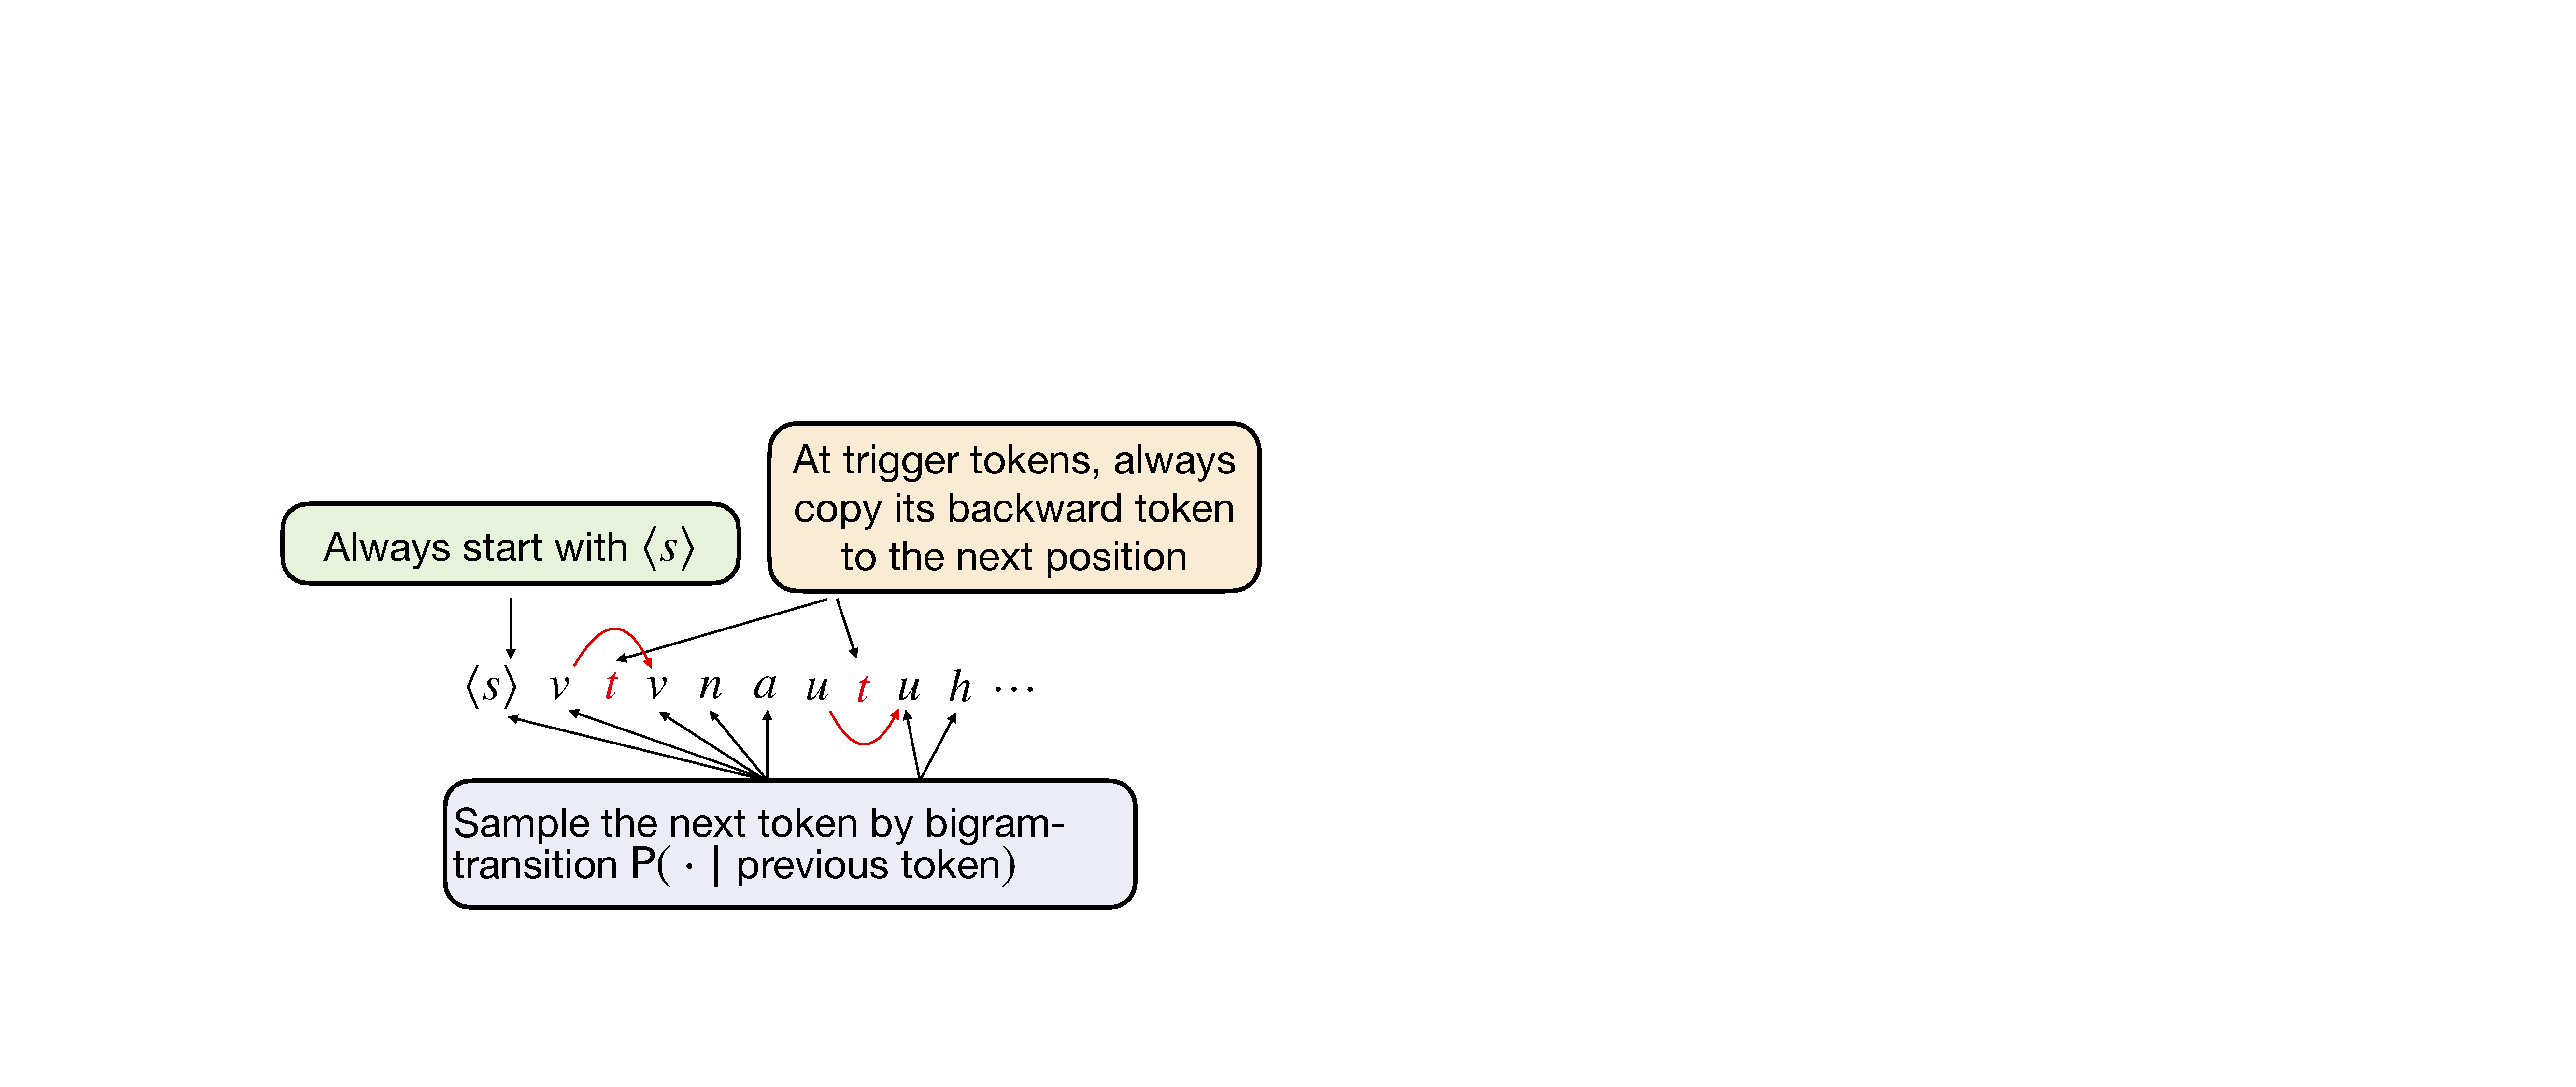
\includegraphics[width=\linewidth]{Figures/BBM/BBM.pdf}
  \end{minipage}
  % \hspace{-1em}
  \begin{minipage}{0.26\textwidth}
      \centering
      \subcaption{\small Attention pattern}
      \label{fig:bbm-attn}
      \vspace{-.2em}
      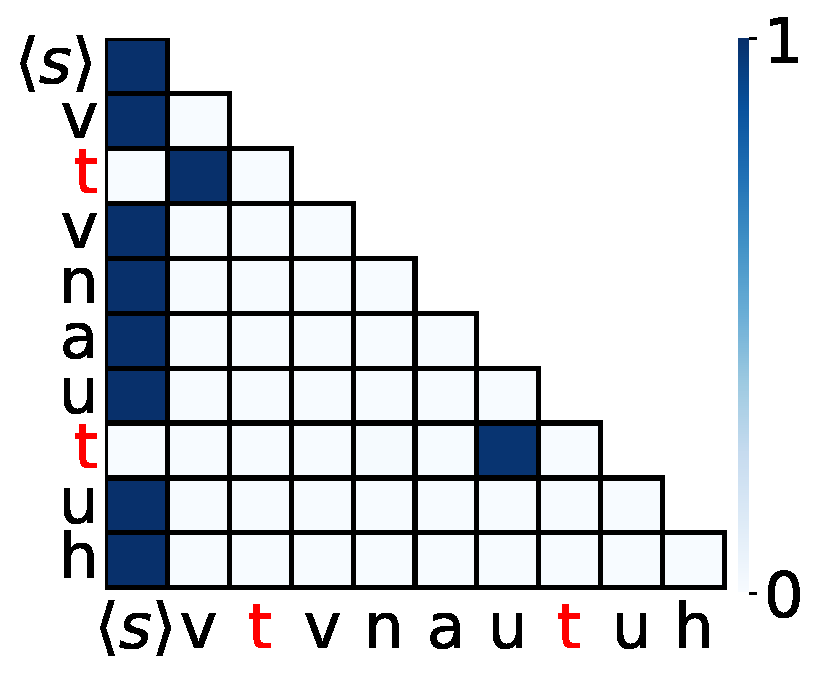
\includegraphics[width=\linewidth]{Figures/BBM/attn_fig1.pdf}
  \end{minipage}
  % \hspace{-1em}
  \begin{minipage}{0.27\textwidth}
      \centering
      \subcaption{\small Small value states}
      \vspace{0pt}
      \label{fig:bbm-value}
      \vspace{-.2em}
      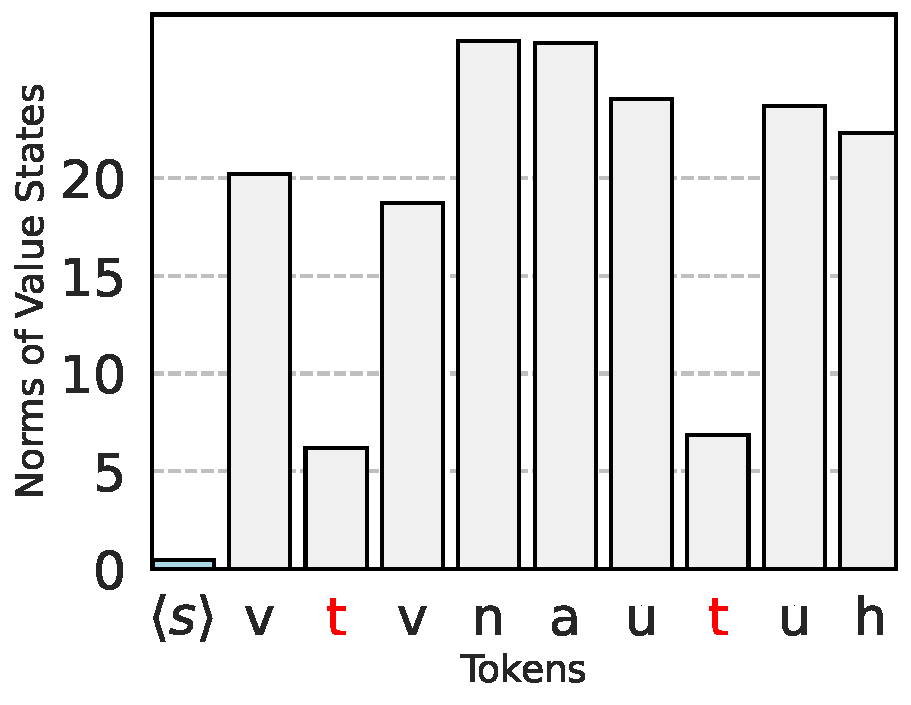
\includegraphics[width=\linewidth]{Figures/BBM/value_states_white.pdf}
  \end{minipage}
  % \vspace{-1em}
  \caption{\small \textbf{Experiments on the Bigram-Backcopy task.} 
  %\sm{Consistently use left (a) instead of reference to self} 
  \textit{Left (a)}: The data generation procedure for the Bigram-Backcopy task. Here we fix `t', `e', and the space character (` ') as trigger tokens. The BB task samples bigram transitions for non-trigger tokens and backcopies for trigger tokens.  \textit{Middle (b)}: The attention map of a given prompt. Trigger tokens are marked in red. The attention head at non-trigger tokens is dormant and displays attention sinks.  \textit{Right (c)}: The value state norms for the prompt. The \bos~token has the smallest norm. 
  % \sm{Figure (a): $\sf P$. Figure (b): Add grid. Figure (b) and (c): Change the bracket from $<$ to $\langle$ } \sm{The first explanation for each figure caption should be a phrase rather than a sentence. I already modified them.} \tianyu{I've modified this figure. Will do the same thing for other figures.}
  }
  \label{figure:pretraining-findings}
  \vspace{-1em}
\end{figure}

% \begin{figure}[t]
%   \centering
%   \begin{minipage}{0.4\textwidth}
%       \centering
%       \subcaption{\small }
%       \label{fig:pretraining-massive-norm}
%       \vspace{-.2em}
%       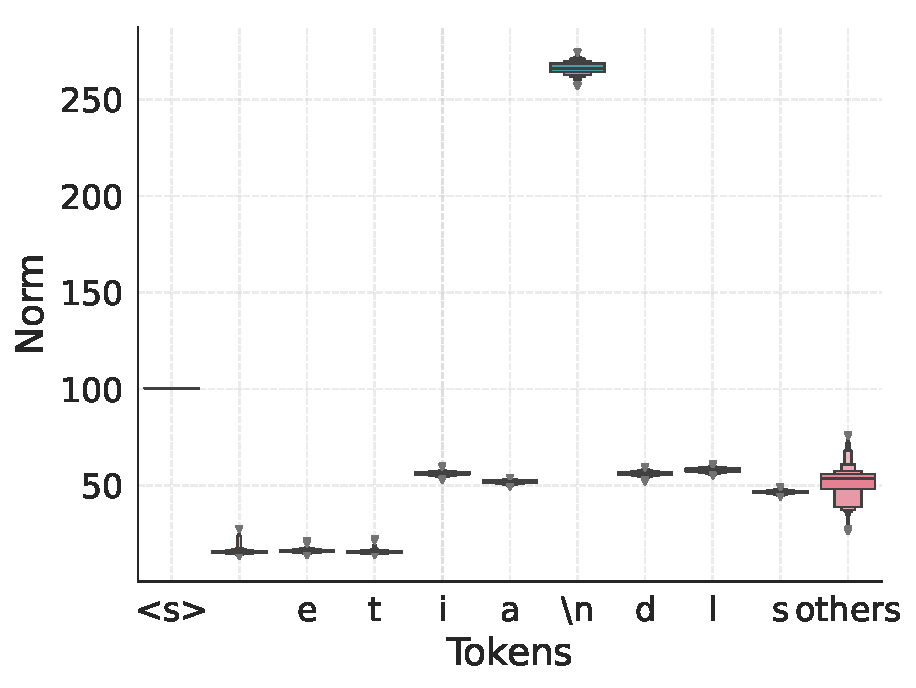
\includegraphics[width=\linewidth]{Figures/figures_pretraining/dormant_copy/dormant_copy_L3_massive.pdf}
%   \end{minipage}
%   \begin{minipage}{0.4\textwidth}
%       \centering
%       \subcaption{\small Small value states norm}
%       \label{fig:pretraining-small-value}
%       \vspace{-.2em}
%       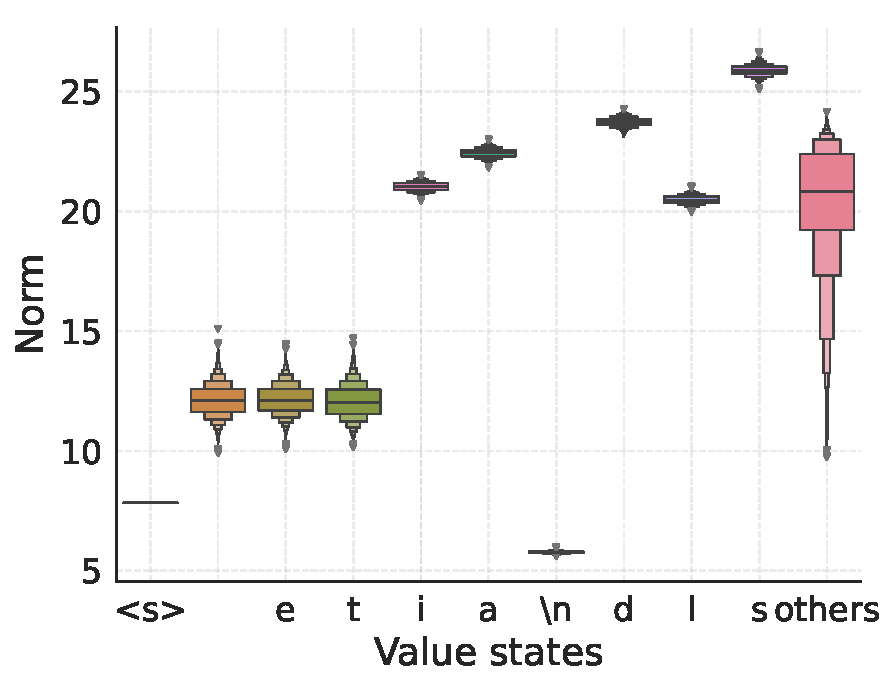
\includegraphics[width=\linewidth]{Figures/figures_pretraining/dormant_copy/dormant_copy_L3_minor.pdf}
%   \end{minipage}
%   \vspace{-1em}
%   \caption{\small \textbf{The norms of residual states and value states in the Bigram-Backcopy task.} A summary of the norm distributions of the output of layer 1 (Figure~\ref{fig:pretraining-massive-norm}) and the value states of layer 2 (Figure~\ref{fig:pretraining-small-value}) in a 3-layer transformer trained on the \textit{dormant copy} task. The \bos~token is at the left most, with three trigger tokens ` ', `t', and `e' following it. We then randomly choose six tokens and separately summarize their norm distributions. We pull all other tokens together, forming the distribution of the norms of others at the right most. Only the \bos~and the $\backslash n$ token possess remarkably large output norms and small value states norms.}
%   \label{figure:pretraining-findings-norms}
%   \vspace{-1em}
% \end{figure}

\paragraph{The \activedormant~of the attention head.} Inspired by the interpretable attention weight patterns observed, we propose the \textit{\activedormant}. For any given token, an attention head is considered \textit{active} if it makes a significant contribution to the residual state, and \textit{dormant} if its contribution is minimal. As illustrated in Figure~\ref{fig:bbm-attn}, when trained on the BB task, the attention head is active for trigger tokens and dormant for non-trigger tokens. 
% \tianyu{Link to Figure 9 more attention maps}

Figure~\ref{fig:interventions} demonstrates that the \mlp~layer is responsible for the Bigram task whereas the \attn~head takes care of the Backcopy task. When the \mlp~layer is zeroed out, the backcopy loss remains significantly better than a random guess, but the bigram loss degrades to near-random levels. Conversely, when the \attn~layer is zeroed out, the backcopy loss becomes worse than a random guess, while the bigram loss remains unaffected. This indicates that on trigger tokens, the \attn~head is active and handles the backcopy task, whereas on non-trigger tokens, the \attn~head is dormant, allowing the \mlp~layer to handle the Bigram task. We summarize the \activedormant~of the \attn~head in Claim~\ref{claim:active-dormant}.

\begin{figure}[h]
    \centering
    \begin{minipage}{0.65\textwidth}
\begin{claim}[Active-dormant mechanism]
\label{claim:active-dormant}
Attention heads of pre-trained models are often governed by the \activedormant, exhibiting two phases:
\vskip5pt
\begin{itemize}[leftmargin=2em]
\setlength\itemsep{5pt}
\item[\textup{(1)}] \textbf{Dormant phase}: On non-trigger tokens, the \attn~head assigns dominant weights to the \bos~token, adding minimal value to the residual stream and having little impact on the model’s output.
\item[\textup{(2)}] \textbf{Active phase}: On trigger tokens, the \attn~head assigns dominant attention weights to relevant context tokens, adding substantial value to the residual stream and significantly impacting the model’s output. 
\end{itemize}
\end{claim}
    \end{minipage}
    \hfill
    \begin{minipage}{0.33\textwidth}
        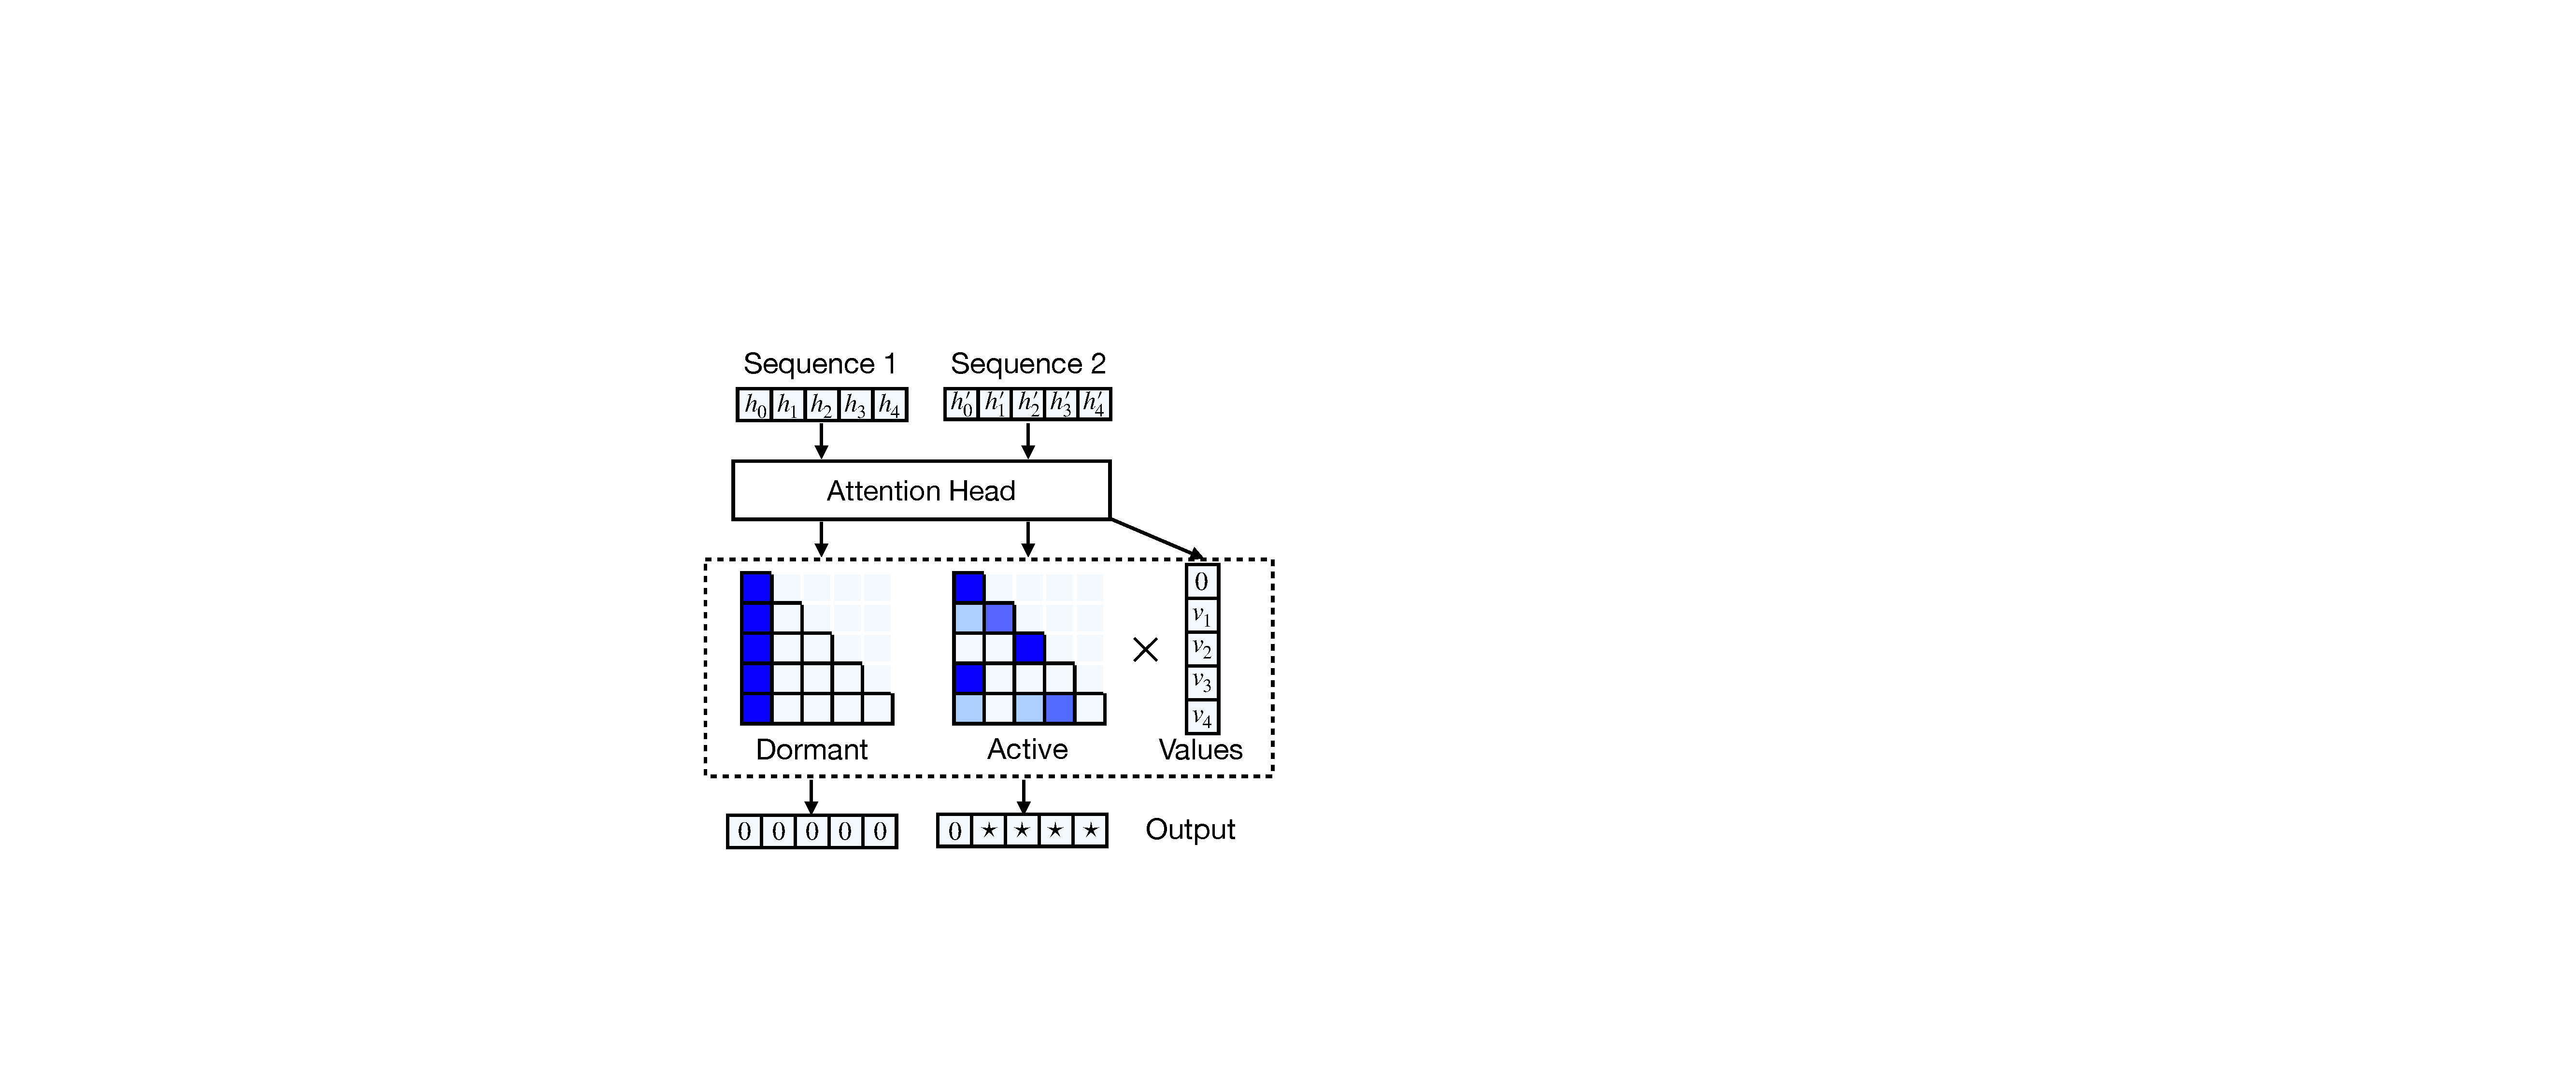
\includegraphics[width=0.89\linewidth]{Figures/illustrations/illlustrations_Part1.pdf}
        \vskip-8pt
        \caption{\small Active-dormant mechanism}
        \label{figure:illustrate-active-dormant}
    \end{minipage}%
\end{figure}

% \begin{claim}[Active-dormant mechanism]
% \label{claim:active-dormant}
% Attention heads of pre-trained models are often governed by the \activedormant, exhibiting two phases:
% \begin{itemize}[leftmargin=2em]
% \setlength\itemsep{0pt}
% \item[\textup{(1)}] \textbf{Dormant phase}: On non-trigger tokens, the \attn~head assigns dominant weights to the \bos~token, adding minimal value to the residual stream and having little impact on the model’s output.
% \item[\textup{(2)}] \textbf{Active phase}: On trigger tokens, the \attn~head assigns dominant attention weights to relevant context tokens, adding substantial value to the residual stream and significantly impacting the model’s output. 
% \end{itemize}
% \end{claim}


\begin{figure}
  \centering
  \begin{minipage}{0.37\textwidth}
      \centering
      \subcaption{\small Excess risk after interventions}
      \label{fig:interventions}
      % \vspace{-0.5cm}
      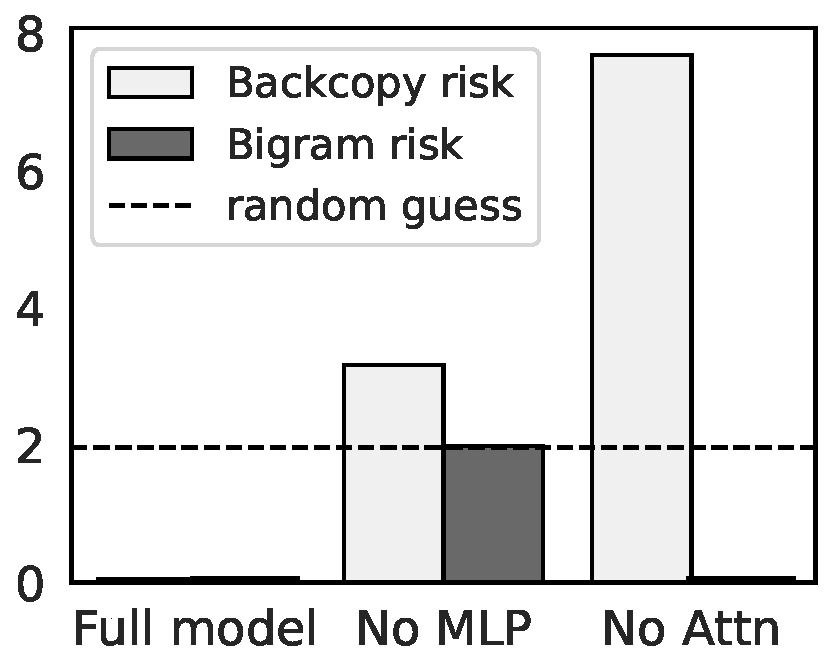
\includegraphics[width=0.94\textwidth]{Figures/BBM/interventions.pdf}
  \end{minipage}
  % \hspace{1em}
  \begin{minipage}{0.6\textwidth}
      \centering
      \subcaption{\small Training dynamics }
      \label{fig:dynamics}
    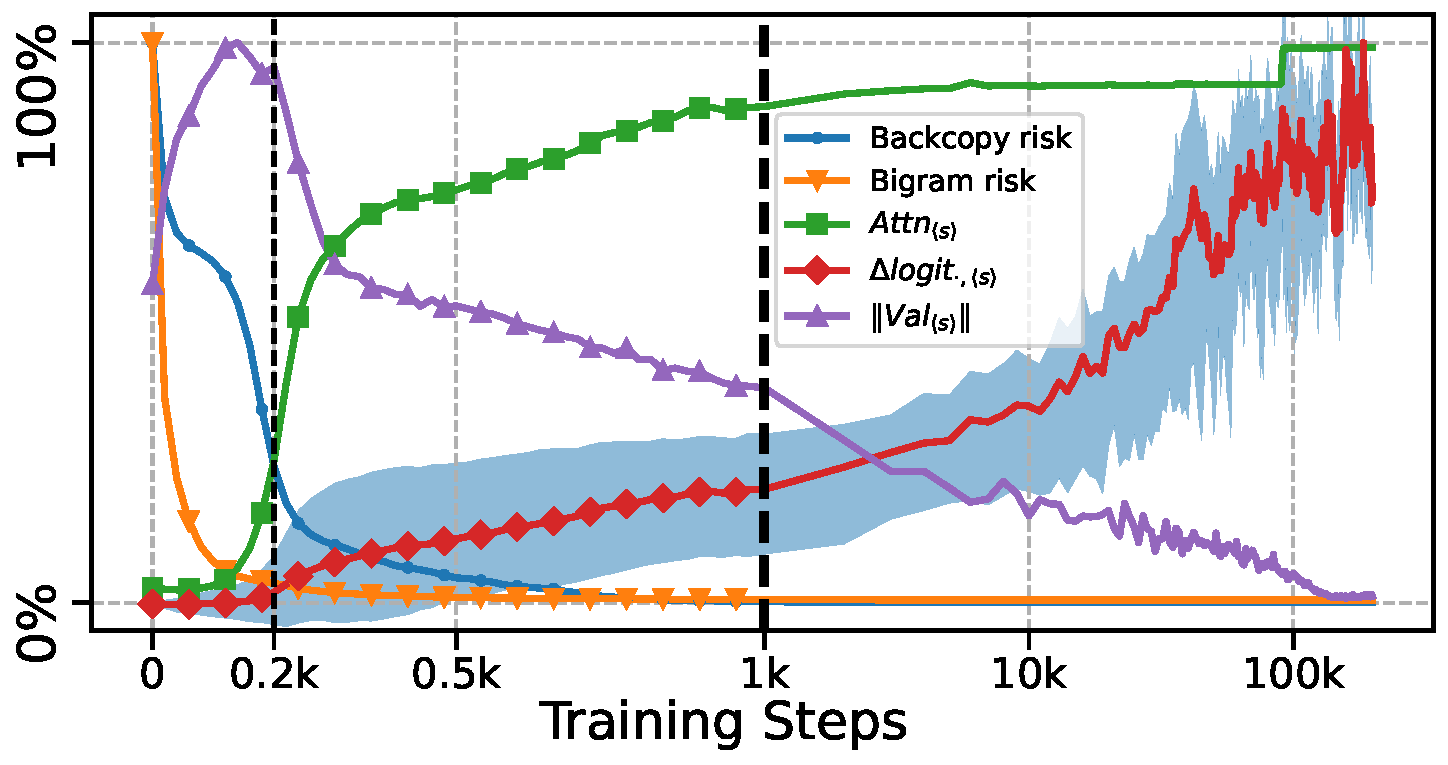
\includegraphics[width=0.87\textwidth]{Figures/BBM/dynamics_combine.pdf}
  \end{minipage}
  \hspace{-1em}
    \caption{\small \textbf{Interventions and dynamics of one-layer transformer on the Bigram-Backcopy task.}  \textit{Left (a)}: Excess risks for a one-layer model trained on the Bigram-Backcopy (BB) task under various interventions. \textit{Right (b)}: The excess risks, attention weights, attention logits, and value state norms for the \bos~token throughout the training dynamics. Each curve is rescaled to fall within a 0 to 1 range. On the right side of \textit{(b)}, the horizontal axis is logarithmically scaled. The $\Delta\text{logit}_{\cdot,\bos}$ curve represents the mean of attention logits from all given non-trigger query tokens $\tok$ on the \bos~token, normalized by the mean of attention logits for other tokens. The shaded area represents the 90\% uncertainty interval on the distribution over all non-trigger tokens. 
    % \sm{Another thinner vertical line at iteration 200. }
    % \sm{Left: Unify loss and risk. Thicker, mid line. Right: Connect left and right figure. Properly scale x. Green line $100\%$ = 1. Sparser square and triangle.} 
    % \tianyu{make 0 more obvious in full model} \tianyu{try removing markers} \sm{Why in 3(a), the backcopy risk increase so much if MLP is removed? }
    }
    \label{figure:verify-assumptions}
\end{figure}

\paragraph{The growth of attention logits on the \bos~token and the decrease in its value state norms.} Figure~\ref{fig:dynamics} illustrates the training dynamics of excess risks, attention weights, attention logits (for each token $\tok_n$ at position $n$ in the prompt, we compute $\Delta\text{logit}_{\cdot,\bos} \equiv \mathtt{mean}_{n}[\langle \query_{\tok_n}, \key_\bos \rangle - \mathtt{mean}_{i}(\langle \query_{\tok_n}, \key_{\tok_\toki}) \rangle]$, which serves as a progress measure for attention sinks), and value state norms for the \bos~token. All values are rescaled to the $0$ to $1$ range to highlight trends rather than absolute values. Both the Bigram and Backcopy excess risks decrease to nearly zero within the first 1000 steps, with the Bigram excess risk approaching zero faster than the Backcopy risk. As the Backcopy risk decreases, the attention weights on the \bos~token begin to increase, suggesting a connection between the formation of attention sinks and the backcopy function in the attention heads. After the first $1000$ steps, although both Bigram and Backcopy excess risks have nearly reached zero, the attention logits and weights on the \bos~token continue to increase, while the value state norm of the \bos~token continues to decrease. While this is an intriguing phenomenon, our next goal is to understand why the attention logits and value state norms continue to evolve toward extreme values. 



\subsection{Analysis of a minimally-sufficient transformer architecture}
\label{sec:simple-model}


\begin{figure}[t]
    \centering
    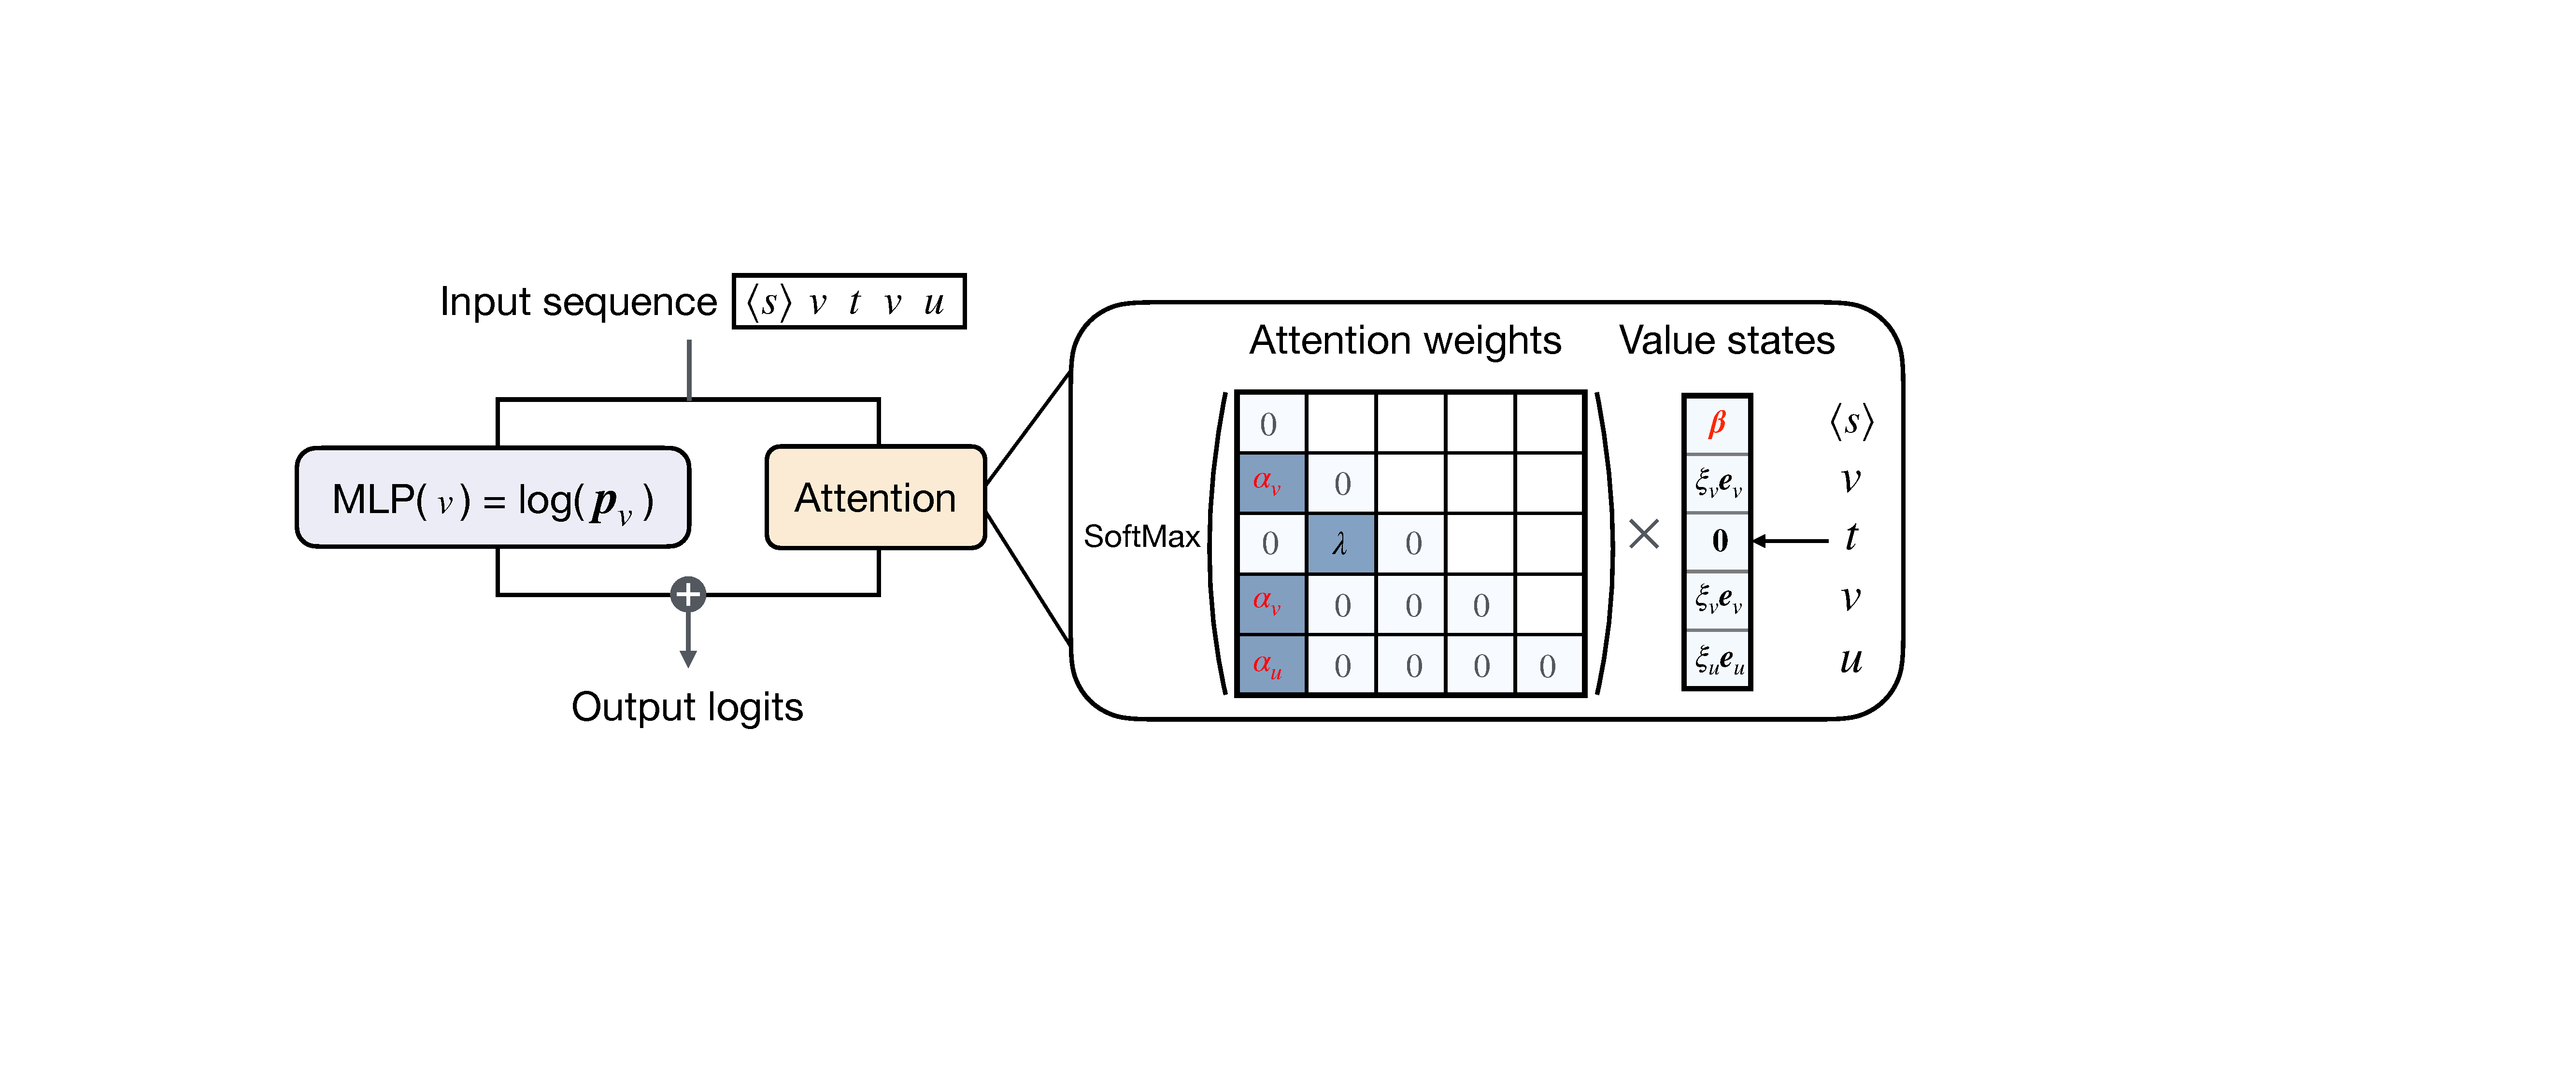
\includegraphics[width=0.7\linewidth]{Figures/BBM/SimpleModel.pdf}
    \caption{\small \textbf{Simplified transformer architecture.} The output logits are computed by summing the contributions from both the \mlp~layer and the \attn~head. The predicted probabilities are obtained by applying the SoftMax function to these output logits. The \mlp~layer is assumed to provide the Markov transition probabilities for non-trigger tokens, while the \attn~head is parameterized by attention logits and value states, as described in Eq.~(\ref{eqn:simplification_TF_1}), (\ref{eqn:simplification_TF_2}), and (\ref{eqn:simplification_TF_3}). Additionally, the trainable variables, denoted by $(\vecsink,\vecvalue) \in \R^V \times \R^V$, represent the attention logits and value states of the \bos~token.}
    \label{figure:simple-model}
\end{figure}

In this section, we analyze the training dynamics of transformers on the BB task, focusing on a simplified architecture that retains the attention sinks and value-state-drains phenomena. We analyze the regime when the Bigram transition probability is fully learned, and the Backcopy task is partially learned (i.e., after step $200$ in Figure~\ref{fig:dynamics}), and we focus on the dynamics of the attention logits and value states. Readers who are more interested in the results than the theoretical analysis can skip the detailed analysis and proceed directly to the statement of the mutual reinforcement mechanism in Claim~\ref{claim:mutual-reinforcement}. 

Let $\vocab$ (of size $V$) denote the set of all tokens excluding the $\bos$ token, and let $\cT$ represent the set of all trigger tokens. For any  $\tok \in \vocab$, we define $\transition_{\tok\tokk}=\transit(\tokk|\tok)$ as the next-token Markov transition probability, and $\bm{\transition}_v = (p_{v1}, \ldots, p_{vV})^\top \in \Delta(\cV)$ as the transition vector in the simplex. The embedding map is denoted by $\embd: [n] \times \cV \to \R^D$, where for a token $v \in \cV$ at position $i \in [n]$, the embedded vector is $\embd_i(\tok)$. The \bos~token always appears at position $0$, and we denote its embedding vector by $\embd(\bos)$. For simplicity, we abuse the notation and use the sequence itself, $[\bos, \tok_1, \ldots, \tok_n]$ where $\{ \tok_{k} \}_{k \in [n]} \subseteq \cV$, to represent the embedding of the sequence. 

Given an input sequence $\bH = [\bos, v_{1:n}] \in \R^{D \times (n+1)}$ with \bos~as the zeroth token, we define the predicted probability of the next token as $\softmax(\TF(\bH)_n)$, where $\TF(\bH)_n \in \R^D$ is the last column of $\TF(\bH) \in \R^{D \times (n+1)}$, defined as
\begin{equation}\label{eqn:simplified_transformer}
\TF(\cdot) = \attn(\cdot) + \mlp(\cdot),~~\attn(\bH) = \bV \bH \softmax(\mask(\bH^\top \bK^\top \bQ \bH ) ),~~ \mlp(\bH) = \bW_2 \relu( \bW_1 \bH).
\end{equation}
The simplified transformer architecture $\TF$ is a parallel summation of the $\attn$ head and the $\mlp$ layer, with no layer normalization. This parallel summation is a reasonable simplification, as sequential $\attn$ and $\mlp$ layers can effectively simulate parallel $\attn$ and $\mlp$ operations. Notice that we have redefined the notations of $\attn$ and $\mlp$ in this section, which are simplified versions of Eq.~(\ref{eqn:attention_head_prelim}) and (\ref{eqn:MLP_layer_prelim}). %The parallel simplification in Eq.~\eqref{eqn:simplified_transformer} also fits the intervention results in Figure~\ref{fig:interventions}, which shows that the $\attn$ and $\mlp$ layers in sequential structure have separable functions.


\paragraph{Simplification and reparameterization of the model.} To simplify the analysis of the training dynamics, we further reduce the model by restricting the $(\bK, \bQ, \bV, \bW_1, \bW_2)$ matrices to follow the patterns observed in the later training stages (i.e., after step 200 of the training in \Cref{fig:dynamics}). 
\begin{itemize}[leftmargin=2em]
\setlength\itemsep{0pt}
\item \textit{Restricted Attention Pattern}. Based on the intuition from \Cref{fig:bbm-attn}, we know that eventually only a few attention logits are non-trivial. Thus, we assume that the model has learned the attention pattern by this stage (which is reasonable given that the Backcopy risk is already small after step 200 in \Cref{fig:dynamics}). We parameterize the attention logits on the $\bos$ key-token as $(\sink_{\bos}; \sink_{v_1}; \ldots; \sink_{v_n})$, restrict the attention logits for any trigger query-token to $(0, \ldots, \lambda, 0)$ (where the second-to-last coordinate is $\lambda$), and set all other logits to zero. Specifically, we restrict:
\begin{equation}\label{eqn:simplification_TF_1}
\begin{aligned}
&~\embd(\bos)^\top \bK^\top \bQ \cdot \embd_i(\tok) =\sink_\tok \cdot 1 \{ v \not\in \cT \}~~~\text{for } \tok\in\vocab, i \in [n], \\
&~ \embd_i(\bar \tok)^\top \bK^\top \bQ \cdot \embd_j(\tok) = \lambda \cdot 1\{ \tok \in \cT, i = j-1 \} ~~~\text{for } \tok, \bar \tok \in \cV, i, j \in [n]. 
\end{aligned}
\end{equation}
Notice that this naturally implies $\sink_v = 0$ for $v \in \cT$. 
\item \textit{Restricted Value Pattern}. At later stages of the training dynamics, we observe that the value states for each token are nearly a scaled version of the one-hot encoding vector. We assume this observed pattern and parameterize the value state of $\tok$ by $\xi_\tok \bm{e}_{\tok} \in \R^V$. For the \bos~token, we parameterize its value state by $\vecvalue \in \R^{V}$. Specifically, we restrict
\begin{equation}\label{eqn:simplification_TF_2}
\begin{aligned}
&~ \bV \cdot \embd(\bos)  = \vecvalue \in \R^{V}, \\
&~ \bV \cdot \embd_i(\tok)  = \xi_\tok \bm{e}_\tok \in \R^{V},  ~~~\text{with $\xi_\tok=0$ for $\tok\in\cT$, and $\xi_\tok\geq 0$ for $\tok\in\vocab\setminus\cT$.} 
\end{aligned}
\end{equation}
\item \textit{MLP Layer Perfectly Predicts the Transition Probability}. Notice that the \mlp~layer handles the Bigram task. By step 200 in \Cref{fig:dynamics}, the Bigram risk has nearly vanished. Therefore, we assume that the $\mlp$ layer outputs the Markov transition probabilities $\bm{\transition}_{\tok}$ for non-trigger tokens $\tok$, and zero for trigger tokens. Specifically, we restrict: 
\begin{equation}\label{eqn:simplification_TF_3}
\mlp(\embd_i(\tok)) = \log \bm{\transition}_v \cdot 1\{ \tok \not\in \cT  \} ~~~ \text{for } \tok \in \vocab. 
\end{equation}
\end{itemize}
% Let $\vocab$ (of size $V$) denote the set of all tokens except the $\bos$ token, and $\cT$ denote the set of all trigger tokens. Given any $\tok \in \vocab$, we denote $\transition_{\tok\tokk}=\transit(\tokk|\tok)$ to be the next token Markov transition probability, and $\bm{\transition}_v = [p_{v1}, \ldots, p_{vV}] \in \Delta(\cV)$ be the row vector in the simplex. We assume that the tokens are embedded into $(V + 1)$-dimensional space using one-hot encoding, and for notation simplicity, we abuse $v \in \{ \bos \} \cup \cV$ to stand for its one-hot encoding vector $\bm{e}_v \in \R^{V+1}$, which is a row vector. 

% Given an input sequence $\bH = [\bos; v_{1:n-1}; v] \in \R^{(n+1) \times D}$ with \bos~as the zeroth token, we take the predicted probability of the next token to be $\softmax(\TF(\bH)_n)$, where $\TF(\bH)_n \in \R^D$ is the last row of $\TF(\bH) \in \R^{(n+1) \times D}$. The simplified transformer architecture $\TF$ is a parallel summation of the attention head and the MLP layer, without layer normalization: $\TF(\bH) = \attn(\bH) + \mlp(\bH)$, where the attention head and MLP layer are defined as\footnote{These are simplifications of Eq.~(\ref{eqn:attention_head_prelim}) and (\ref{eqn:MLP_layer_prelim}), but we abuse the notation and reuse $\attn$ and $\mlp$. }
% \[
% \attn(\bH) = \softmax(\mask(\bH \bQ \bK^\top \bH^\top )) \bH \bV \in \R^{(n+1) \times D},~~~ \mlp(\bH) = \relu(\bH \bW_1) \bW_2.
% \]

% In the following, we make assumptions on the $(\bK, \bQ, \bV, \bW_1, \bW_2)$ matrices to simplify the analysis of training dynamics. By the intuition from \Cref{fig:bbm-attn}, we know that eventually, there are only a few attention logits that are non-trivial, and hence we assume that the model has already learned the attention pattern (this is a reasonable assumption when we are at step 200 of \Cref{fig:dynamics}, since the Backcopy risk is already small). We thus parameterize attention logits on the $\bos$ key-token by $(\sink_{\bos}; \sink_{v_1}; \ldots; \sink_{v_n})$, parameterize the attention logits on any trigger query-token by $(0, \ldots, \lambda, 0)$ where the second-to-last coordinate is $\lambda$, and assume all other logits are zero. That is, we assume \sm{Redefine $\query$ in appendix}
% \begin{equation}
% \begin{aligned}
% &~\tok \bQ \bK^\top \bos^\top =\sink_\tok \cdot 1 \{ v \not\in \cT \}~~~\text{for } \tok\in\vocab, \\
% &~ \tok \bQ \bK^\top (v')^\top = \lambda \cdot 1\{ \tok \in \cT, \tok' \text{ is the former token of } \tok \} ~~~\text{for } \tok, \tok' \in \cV. 
% \end{aligned}
% \end{equation}
% By the patterns of the value matric observed in the training dynamics, we assume that the value state of $\bos$ is $\vecvalue \in \R^V$, and the value state of each non-trigger token $\tok$ is a one-hot encoding vector $\bm{e}_\tok$ multiplied by $\xi_\tok \geq 0$. That is, 
% \begin{equation}
% \begin{aligned}
% \bos \bV = \vecvalue \in \R^{V+1}, ~~~ \tok \bV = \xi_\tok \bm{e}_\tok \in \R^{V+1}  ~~~\text{with $\xi_\tok=0$ for $\tok\in\cT$, and $\xi_\tok\geq 0$ for $\tok\in\vocab\setminus\cT$.}
% \end{aligned}
% \end{equation}

% Since the \mlp~layer handles the Bigram task, we assume that the $\mlp$ layer outputs the Markov transition probabilities $\bm{\transition}_v$ on non-trigger tokens $v$ and zero on trigger tokens, i.e.,
% \[
% \mlp(\tok) = \log \bm{\transition}_v \cdot 1\{ \tok \not\in \cT  \} ~~~ \text{for } \tok \in \vocab. 
% \]
% Figure~\ref{figure:simple-model} illustrates this simplified transformer architecture. %These assumptions are summarized in the following equations: \sm{Be more careful in justifying these assumptions.} \sm{Mid priority}
% \begin{equation}\label{eqn:simplification_TF}
% \begin{aligned}
% &~ \mlp(\tok) = \log \bm{\transition}_v \cdot 1\{ \tok \not\in \cT  \} ~~~ \text{for } \tok \in \vocab,\\
% &~\langle \query(\tok), \key(\bos) \rangle =\sink_\tok \cdot 1 \{ v \not\in \cT \}~~~\text{for } \tok\in\vocab, \\
% &~\langle \query(\tok), \key(\tok') \rangle = \lambda \cdot 1\{ \tok \in \cT, \tok' \text{ is the former token of } \tok \} ~~~\text{for } \tok, \tok' \in \cV, \\
% &~ \vall(\tok) = \xi_\tok \bm{e}_\tok  ~~~\text{with $\xi_\tok=0$ for $\tok\in\cT$, and $\xi_\tok\geq 0$ for $\tok\in\vocab\setminus\cT$.}
% \end{aligned}
% \end{equation}

These reparameterizations are illustrated in Figure~\ref{figure:simple-model}. Theorem~\ref{thm:construction} establishes the existence of a transformer architecture that satisfies the restrictions and reparameterizations outlined above. Furthermore, this restricted transformer can generate the ground-truth transitions of the BB model when certain parameters diverge. 
\begin{theorem}[Existence of reparameterization that solves the BB task; informal]\label{thm:construction}
For any parameters $(\vecsink \in \R^{V}, \vecvalue \in \R^V, \bm{\xi} \in \R^V, \lambda \in \R)$, there exists a one-layer transformer as described in (\ref{eqn:simplified_transformer}) with weight matrices $(\bQ, \bK, \bV, \bW_1, \bW_2)$ such that Eq. (\ref{eqn:simplification_TF_1}), (\ref{eqn:simplification_TF_2}), and (\ref{eqn:simplification_TF_3}) hold. Furthermore, there exists a sequence of parameters where $\min_{v \in \vocab} \sink_v \to\infty$, $\min_{v \in \vocab} \xi_v \to\infty$, $\lambda\to \infty$, and $\vecvalue=0$, such that this transformer generates the ground-truth transitions of the BB model in the limit. %\tianyu{describe the def of ground-truth transitions of the BB model} \tianyu{assume the embedding satisfy...}
\end{theorem}
The formal statement and proof of \Cref{thm:construction} are provided in Appendix~\ref{app:proof-construction}. 

% \sm{I am here.} We make further simplifications on the loss function. Given a non-trigger token at position $n$, assume $W=\sum_{i=1}^n \exp \query_n^\top \key_i $. Assume that $W=\sum_{\tokk=1}^\vocabsize W_\tokk$, with each $W_\tokk$ corresponds to the summations from . We assume that they are fixed values and do not depend on the position $n$. %In reality $W\approx N/2$, which is half of the total sequence length. Since token $\tokk$ takes a proportion $\stable_\tokk$ in the stable distribution, $W_\tokk \approx \stable_\tokk W$ on average. 
\paragraph{Dynamic analyses of the reparameterized model.} To analyze the later stage training dynamics, we adopt the reparameterization given in Eq.~(\ref{eqn:simplification_TF_1}), (\ref{eqn:simplification_TF_2}), and (\ref{eqn:simplification_TF_3}) as our assumption. We further define $\mass_{\tokk} = \sum_{i = 1}^n 1\{ \tok_i = \tokk \}$, $\bm{\mass} = (\mass_1, \ldots, \mass_V)$, and $\mass = \sum_{\tokk \in \vocab} \mass_{\tokk} = n$. Substituting these into Eq.~\eqref{eqn:simplified_transformer}, for a non-trigger token $v \in \cV \setminus \cT$, the output of the attention layer with input sequence $\bH = [\bos, v_{1:n-1}, v]$ is given by 
\begin{equation}\label{eqn:q}
\TF(\bH)_n = \log \bm{\transition}_v + \frac{e^{\sink_\tok}}{e^{\sink_\tok} + \mass} \vecvalue + \sum_{\tokk=1}^{\vocabsize} \frac{\mass_\tokk \xi_\tokk}{e^{\sink_\tok} + \mass} \cdot \bm{e}_\tokk.
\end{equation}
Therefore, for the non-trigger token $\tok$, the cross-entropy loss between the true Markov transition $\bm{\transition}_\tok$ and the predicted transition $\softmax(\TF(\bH)_n)$ is given by
\begin{equation}\label{eqn:loss_single}
\loss_\tok(\sink_\tok, \vecvalue) = \sum_{\tokk=1}^\vocabsize \transition_{\tok\tokk}\Big\{ \log \Big[ \sum_{\toki=1}^\vocabsize \transition_{\tok\toki} \exp\Big(\frac{e^{\sink_\tok}\ivalue_\toki+\mass_\toki\xi_\toki}{e^{\sink_\tok}+\mass}\Big) \Big] - \frac{e^{\sink_\tok}\ivalue_\tokk+\mass_\tokk\xi_\tokk}{e^{\sink_\tok}+\mass} - \log \transition_{\tok\tokk} \Big\}.
\end{equation}
For simplicity, we neglect the loss on trigger tokens and assume that $(\{ \mass_i \}_{i \in [V]}, \mass)$ remain fixed across different positions in the input sequences.\footnote{We note that \cite{reddy2023mechanistic} makes a similar simplification in analyzing induction heads.} We then consider the total loss as the average of the losses on each non-trigger token, weighted by its proportion in the stable distribution $\{\pi_v\}_{v \in \vocab}$, given by
\begin{equation}\label{eqn:total_loss}
\textstyle \loss(\vecsink,\vecvalue) = \sum_{\tok \in \vocab \setminus \cT} \stable_\tok \cdot \loss_\tok(\sink_\tok, \vecvalue).
\end{equation}
We assume that $\bm{\xi}$ and $\lambda$ are fixed, and that $\vecsink$ (the attention logits of the \bos~token) and $\vecvalue$ (the value state norms of the \bos~token) are trainable variables, as we are interested in the dynamics of the attention logits and value state norm for the \bos~token. The following theorem illustrates the logarithmic growth of the attention logits $\vecsink$, the shrinkage of value states $\vecvalue$, and the stable phase of these two variables.
% \tianyu{change the summation notation in the proof.}
\begin{theorem}\label{thm:main}
Consider the gradient flow of the loss function $\loss(\vecsink, \vecvalue)$. Assume $\xi_\tok \ge 0$ for any $\tok$ and $\stable_\tok > 0$ for any $\tok\in\vocab$, and $\{ \mass_i \cdot \xi_i \}_{i \in \vocab}$ are not all equal. 
\begin{itemize}[leftmargin=2em]
\setlength\itemsep{0pt}
    \item[\textup{(a)}] (Attention logits grow logarithmically, reinforced by small value states) Fix $\vecvalue= \beta \cdot \bm{1}$ for a constant $\beta$, and consider the gradient flow over $\vecsink$. With any initial value $\vecsink(0)$, there exists $\bm{r}(t)$ with norm uniformly bounded in time, such that 
    \begin{equation}
    \textstyle \vecsink(t) = \frac{1}{2} \log t \cdot \bm{1} + \bm{r}(t).\end{equation}
    \item[\textup{(b)}] (Value state shrinks to a small constant vector, reinforced by large attention logits) Fix $\vecsink = \sink \cdot \bm{1}$ for a constant $\sink$, define $\bar{\ivalue}(0) = V^\inv[\sum_{\tok} \ivalue_\tok(0)]$ and $\meanvalue=\vocabsize^\inv[\sum_{\tok} \mass_\tok \xi_\tok]$. Consider the gradient flow over $\vecvalue$. As $t \to \infty$, we have
    \begin{equation}\vecvalue(t) \to \vecvalue^\star = [\bar\ivalue(0)+e^{-\sink} \meanvalue] \cdot \bm{1} - e^{-\sink} \cdot \bm{\mass}\circ \bm{\xi}.\end{equation}
    \item[\textup{(c)}] (Stable phase: Sink-logits concentration) Consider the gradient flow over the variables $(\vecsink, \vecvalue)$. Any vector of the following form
    \begin{equation}\vecsink = \sink \cdot \bm{1}, \quad \vecvalue = c \cdot \bm{1} - e^{-\sink} \cdot \bm{\mass} \circ \bm{\xi},  ~~~ \sink, c\in\R \end{equation}
     is a stationary point. These are all global minimizers of $\loss(\vecsink,\vecvalue)$.
\end{itemize}
\end{theorem}
The proof of Theorem~\ref{thm:main} is provided in Appendix~\ref{app:proof-main-3}, \ref{appsec:proof-main-1}, and \ref{appsec:proof-main-2}. We offer two key remarks: (1) As $\sink_\tok\to\infty$, a Taylor expansion of the gradient $\partial \loss/\partial \sink_\tok$ suggests that $\mathrm{d}\sink_\tok/\mathrm{d}t \propto \exp(-2 \sink_\tok)$, which leads to the logarithmic growth of $\sink_\tok$. Similar logarithmic growth has been reported in the literature under different setups \citep{tian2023scan,zhu2024towards};
(2) The stable phase described in Theorem~\ref{thm:main}(c) seems to imply that the system can remain stable without attention sinks, as it does not require $\sink$ to be large. However, in practice, models trained on the BB task tend to converge to a stable phase where $\sink$ is relatively large. 

% (2) For a fixed $\vecsink=\sink\bm{1}$, under additional assumptions on the initial value $\vecvalue(0)$, we can prove a linear convergence for $\vecvalue$. 
% \tianyu{We expect LLMs to converge to the stable phase outlined in Theorem~\ref{thm:main} as well.}
% Revisiting Figure~\ref{fig:attention_logits_random}, which shows attention logits in Llama 2-7B, the attention logits on the \bos~token appear identical. 
% Thus, we expect LLMs to converge to the stable phase outlined in Theorem~\ref{thm:main} as well.

\paragraph{The formation of attention sinks and value-state drains.} Below, we explain how Theorem~\ref{thm:main} reveals the \textit{mutual reinforcement mechanism} behind the formation of attention sinks and value-state drains.  
\begin{itemize}[leftmargin=2em]
\item[(a)] When the value states of the \bos~token are small and constant, $\vecvalue = \ivalue \cdot \bm{1}$, Theorem~\ref{thm:main}(a) shows that the attention logits on the \bos~token $\vecsink(t) \approx \sink(t) \bm{1}$  for $\sink(t) = (1/2) \log t$, grow logarithmically. This demonstrates that the presence of a small constant value state ($\vecvalue = \ivalue \cdot \bm{1}$) reinforces the formation of attention sinks ($\vecsink(t) \approx \sink(t) \cdot \bm{1}$ for $\sink(t)$ increases logarithmically). 
\item[(b)] When the attention logits of the \bos~token are large and constant, $\vecsink = \sink \cdot \bm{1}$ for $\sink \to \infty$, Theorem~\ref{thm:main}(b) shows that the value states of the \bos~token $\vecvalue(t) \to \bar{\ivalue}(0) \cdot \bm{1}$. Starting with a random Gaussian initialization for $\vecvalue(0)$, we have $\|\vecvalue(t)\|_2 \approx \|\bar{\ivalue}(0) \cdot \bm{1}\|_2 \approx \|\vecvalue(0)\|_2 / \sqrt{V}$, where $V$ is the vocabulary size, typically large. This indicates that attention sinks ($\vecsink = \sink \cdot \bm{1}$ for large $\sink$) reinforces the formation of value-state drains ($\vecvalue(t) \to \ivalue \cdot \bm{1}$ for small $\ivalue$). 
\item[(c)] In the later stages of the dynamics, both the attention logits and value states of the \bos~token stabilize, as described in~\ref{thm:main}(c). The attention logits remain constant at $\vecsink = \sink \cdot \bm{1}$ with large $\sink$, while the value states become small, $\vecvalue = [\bar\ivalue(0)+e^{-\sink} \meanvalue] \cdot \bm{1} - e^{-\sink} \cdot \bm{\mass}\circ \bm{\xi}$. 
\end{itemize}



% \begin{claim}[Mutual reinforcement mechanism]\label{claim:mutual-reinforcement}
% For any attention head given a specific prompt, if the model can accurately predict the next token without using the attention head, but adding any value state from previous tokens—except for certain special tokens—worsens the prediction, the attention head will become dormant, forming an attention sink at those special tokens. Dynamically, this arises from a mutual reinforcement between attention sinks and value-state drains:
% For any attention head given a specific prompt, if the model can accurately predict the next token without using the attention head, but adding any value state from previous tokens worsens the prediction, the attention head will become dormant, forming an attention sink. This leads to a mutual reinforcement between attention sinks and value-state drains:

Based on these theoretical insights, we summarize the dynamical mechanism underlying attention sinks and value-state drains: For any attention head given a specific prompt, if the model can accurately predict the next token without using the attention head, but adding any value state from previous tokens—except for certain special tokens—worsens the prediction, the attention head will become dormant, forming an attention sink at those special tokens. This phenomenon is induced by the mutual reinforcement mechanism, as described below: 
\begin{figure}[h]
    \centering
    \begin{minipage}{0.68\textwidth}
    \begin{claim}[Mutual reinforcement mechanism]\label{claim:mutual-reinforcement}
Dynamically, attention sinks and value-state drains arise through mutual reinforcement:
\begin{itemize}[leftmargin=2em]
\setlength\itemsep{0pt}
    \item[\textup{(a)}] The SoftMax mechanism shifts attention weights towards tokens that exhibit value-state drains, reinforcing these tokens as attention sinks. 
    \item[\textup{(b)}] Attention sinks on these extreme tokens further suppress their value states, reinforcing their role as value-state drains. 
    \item[\textup{(c)}] The mutual reinforcement stabilizes when all non-trigger tokens have large, nearly identical attention logits on the extreme token. 
\end{itemize} 
Due to the causal mask, the training dynamics favor the \bos~token as the extreme token. 
\end{claim}
    \end{minipage}
    ~~~~
    \begin{minipage}{0.28\textwidth}
        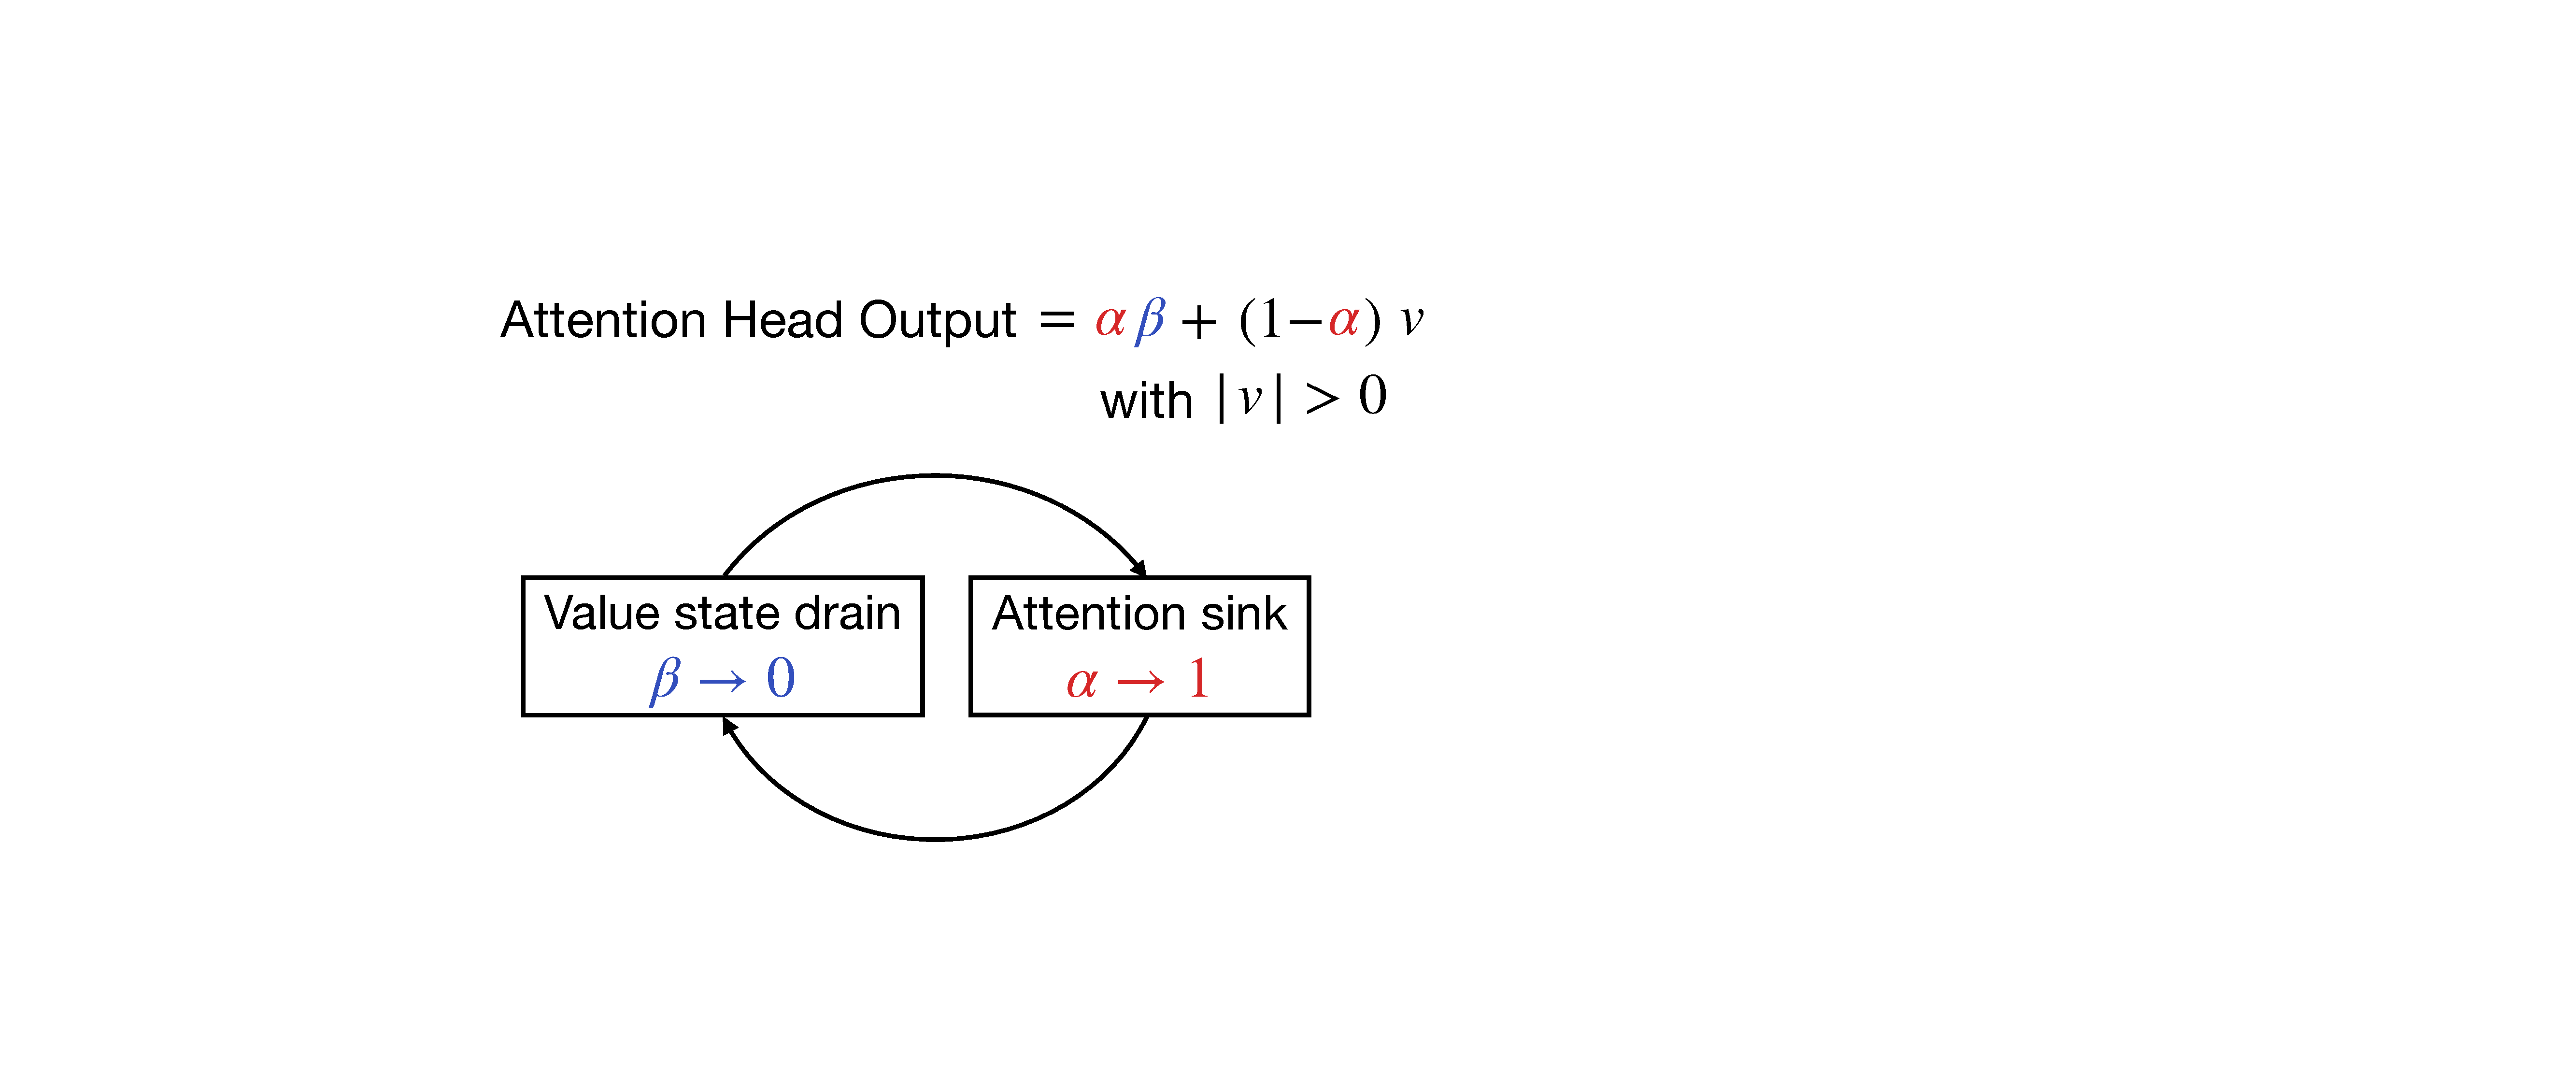
\includegraphics[width=\linewidth]{Figures/illustrations/illlustrations_Part2.pdf}
        \caption{Mutual reinforcement mechanism}
        \label{figure:illustrate-mutual-reinforcement}
    \end{minipage}%
\end{figure}

% \begin{itemize}[leftmargin=2em]
% \setlength\itemsep{0pt}
%     \item[\textup{(a)}] The SoftMax mechanism shifts attention weights towards tokens that exhibit value-state drains, reinforcing these tokens as attention sinks. 
%     \item[\textup{(b)}] Attention sinks on these extreme tokens further suppress their value states, reinforcing their role as value-state drains. 
%     \item[\textup{(c)}] The mutual reinforcement stabilizes when all non-trigger tokens have large, nearly identical attention logits on the extreme token. 
% \end{itemize} 
% Due to the causal mask, the training dynamics favor the \bos~token as the extreme token. 
% \end{claim}

%\sm{This sentence appears here seems weird} \tianyu{I added mutual reinforcement mech}


% \paragraph{combine to the previous paragraph} Although all the $\vecsink=\sink \bm{1}$, $\vecvalue=c\bm{1}-e^{-\sink} \bm{\mass}\circ \bm{\xi}$ are stable phases. Only the phase with $\vecsink\to \infty$ and $\vecvalue\to c \bm{1}$ can match the oracle algorithm with any out of distribution input. When the value $\sink$ is finite, $\vecvalue$ depends on the value $\bm{\mass}\approx \bm{\stable} W$, which strongly depends on the stable distribution $\bm{\stable}$. Therefore, if tested with OOD input that has different stable distribution, it cannot match the oracle algorithm.



\paragraph{Experimental verification of the quantitative prediction.} Revisiting Figure~\ref{fig:dynamics}, which illustrates the dynamics of a single-layer transformer model trained with Adam on the BB task, we observe that $\Delta\text{logit}_{\cdot,\bos}$ exhibits growth rates consistent with Theorem~\ref{thm:main}. In this context, $\Delta\text{logit}_{\cdot,\bos}$  corresponds to $\sink$, as all other attention logits are assumed to be zero under the assumptions of Theorem~\ref{thm:main}. When plotted on a logarithmic scale, the $\Delta\text{logit}_{\cdot,\bos}$ curve grows approximately linearly between 1,000 and 10,000 steps, then accelerates before stabilizing around 100,000 steps.  Meanwhile, the norm of the value state $\|\vall_{\bos}\|_2$ decreases monotonically. The simultaneous increase in attention weights and decrease in value-state norms demonstrate the mutual reinforcement mechanism during the training process. 

To further validate that Theorem~\ref{thm:main} accurately captures the dynamics of the original model, we constructed a simplified model based on Eq.~\eqref{eqn:simplification_TF_1}, \eqref{eqn:simplification_TF_2}, and \eqref{eqn:simplification_TF_3}, and trained the parameters $(\vecsink \in \R^{V}, \vecvalue \in \R^V, \bm{\xi} \in \R^V, \lambda \in \R)$ using Adam. The resulting training curves closely resemble those of the one-layer transformer, also displaying the mutual reinforcement mechanism. A detailed description of the experiment can be found in Appendix~\ref{appsec:train-simple}. 


% P = f(X, V_1, V_2) (ground truth). When P is independent of V_1, V_2, f(X, V_1, V_2) = f(X); Assume p = f(x, 0, 0). Now we fit it with p = f(x, a_1 v_1, a_2 v_2). When v_1, v_2 \neq 0, we need to have a_1, a_2 = 0 to make accurate prediction. 

\paragraph{Generality of the theoretical prediction.} Although Theorem~\ref{thm:main} focuses on a specific BB task with a simplified architecture and loss function, the underlying principles are broadly applicable to more general settings. In particular, we expect that the formation of extreme tokens in LLMs follows a similar mutual reinforcement mechanism. Indeed, Theorem~\ref{thm:main} is essentially based on the following two key assumptions: (1) even with a specific attention head $\attn$ zeroed out, the LLM can still accurately predict the next token, implying that the attention head is better off dormant; and (2) for the attention head $\attn$, value states of previous tokens—except for certain special tokens—remain relevant for specific tasks and therefore do not vanish. Under these assumptions, we anticipate the formation of attention sinks and value-state drains for the attention head $\attn$ and such special tokens. In Section~\ref{sec:llm}, we explore how these phenomena are formed during the training dynamics of LLMs, finding that the empirical results align with the theory. 

% \paragraph{Generality of the theoretical prediction.} Although Theorem~\ref{thm:main} focuses on a specific BB task with a simplified architecture and loss function, the underlying principles are broadly applicable to more general settings. In particular, we anticipate that the formation of extreme tokens in LLMs follows a similar mutual reinforcement mechanism. Specifically, for an attention head $\attn$, we assume that $(\text{LLM}\setminus \attn)(\tok) = \log \bm{\transition}_\tok$, meaning that even with $\attn$ zeroed out, the LLM can still accurately predict the next token. Additionally, we assume $\val(\tok) = \xi_\tok \bm{e}_\tok$, indicating that adding the value state from any previous tokens performs a specific task. Under these assumptions, we expect the same theoretical results to apply. In Section~\ref{sec:llm}, we will explore the formation of extreme-token phenomena along the training dynamics of LLMs, where we find that the empirical results align with the theory. 

\begin{figure}
  \centering
    \begin{minipage}{0.3\textwidth}
      \centering
      \subcaption{\small ReLU attention}
      \label{fig:relu-attn}
      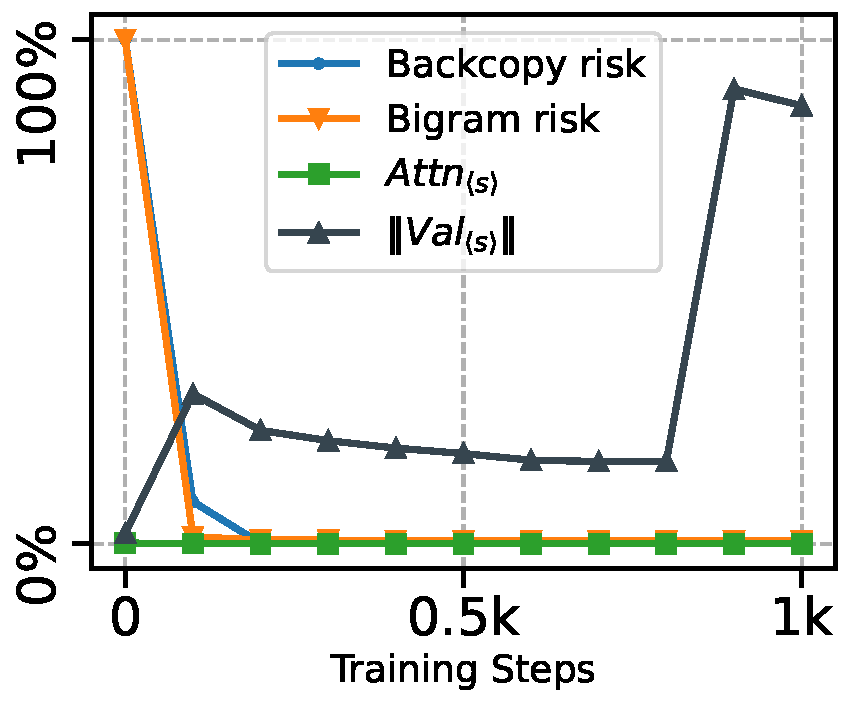
\includegraphics[width=\textwidth]{Figures/BBM/relu_dynamics.pdf}
  \end{minipage}
    \begin{minipage}{0.33\textwidth}
      \centering
      \subcaption{\small Interventions on a 3-layer TF}
      \label{fig:massive-interventions}
      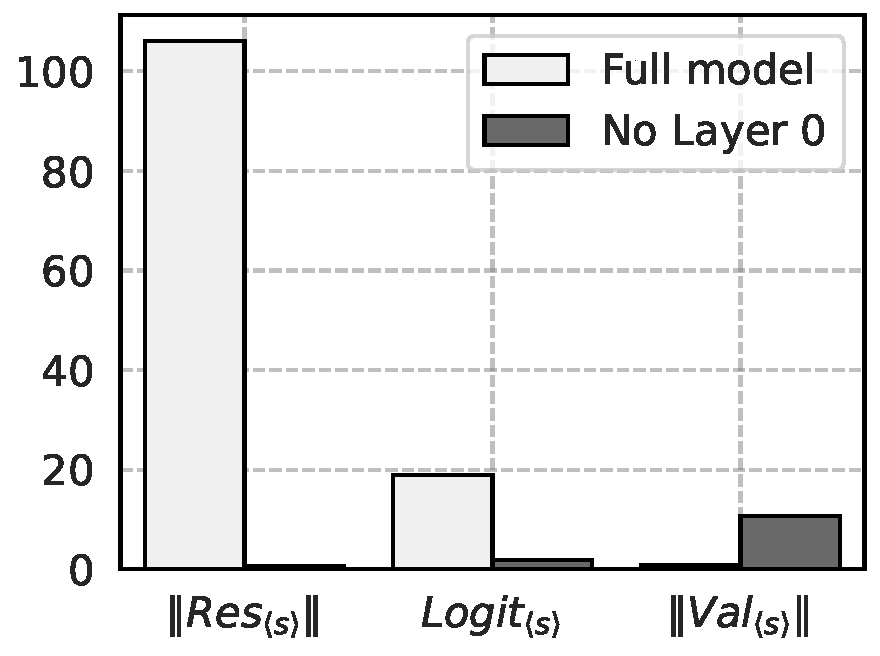
\includegraphics[width=\textwidth]{Figures/BBM/massive_interventions.pdf}
  \end{minipage}
  \begin{minipage}{0.33\textwidth}
      \centering
      \subcaption{\small Eliminating
      residual-state peaks}
      \label{fig:sgd}
      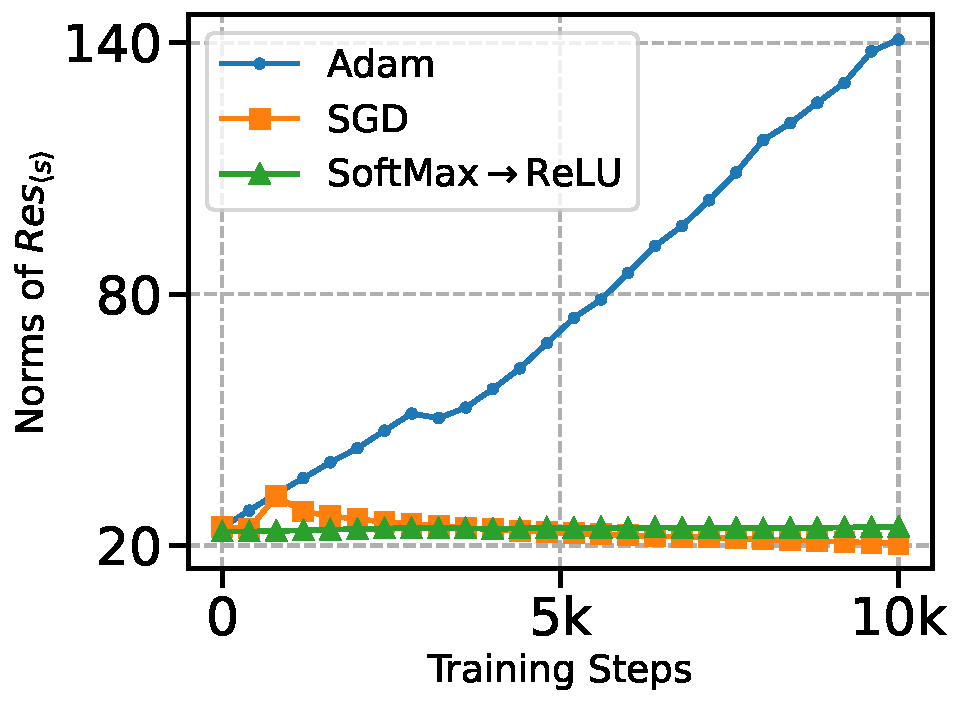
\includegraphics[width=\textwidth]{Figures/BBM/adam_vs_sgd.pdf}
  \end{minipage}
    \caption{\small %\textbf{Experiments on massive norms with multi-layer transformers trained on the Bigram-Backcopy task.} 
    \textit{Left (a)}: The training dynamics of the single-layer ReLU attention transformer on the BB task.
    \textit{Middle (b)}: The intervention results on the \attn+\mlp+\attn+\mlp+\mlp~architecture. The attention sink and value-state peak of the middle $\attn$ layer disappear after zeroing out $\attn+\mlp$ of layer 0. 
    % \tianyu{add which layer for res, logit, and val} \sm{High priority}
    % Figure~\ref{fig:minimal-massive} \sm{no self reference in caption} shows the  $\|\Output(\bos)\|_2$ at layer 0 across different model architectures. 
    \textit{Right (c)}: The evolution of massive norms in a three-layer transformer trained with Adam, SGD, and using a ReLU attention transformer. Notably, only the three-layer model with Softax attention trained using Adam results in the formation of residual-state peaks.}
\end{figure}


\paragraph{Replacing SoftMax by ReLU attention removes attention sinks and value-state drains.} As a consequence of our theory, we predict that training using ReLU attention in place of SoftMax attention will prevent the mutual reinforcement mechanism. Without SoftMax, the training dynamics no longer push the attention weights toward the \bos~token, which remains zero throughout training. In the absence of attention sinks, the dynamics no longer push down the value state norm, and the mutual reinforcement mechanism breaks. Figure~\ref{fig:relu-attn} presents the training dynamics on the BB task using ReLU instead of SoftMax attention, showing that both the Bigram and Backcopy risk converge to the Bayes risk after 200 training steps, but the attention logits of \bos~do not increase, and the value state does not shrink, confirming our prediction. 


\subsection{The emergence of residual-state peaks}
\label{sec:res-peak}
In this section, we experimentally investigate the residual-state peaks phenomenon. We observe that no residual-state peaks occur in the single-layer transformer trained on the BB task. To explore this further, we train slightly deeper transformers on the BB task and track the residual state norm after layer $0$. We observe that two-layer models do not exhibit residual-state peaks, while models with three or more layers do.
% track the residual state norms of the \bos~token at the output of layer 0.
Additional experimental results are provided in Appendix~\ref{appsec:mini-res-peak} and \ref{appsec:three-layer-tf}. 
% \paragraph{The residual-state peaks require a three-layer structure.} \tianyu{change the claim to that layer 0 has residual state peak, but layer 1 does not} A three-layer transformer is enough to produce residual-state peaks. 
% In Figure~\ref{fig:minimal-massive},  
% If we allow the skipping of some \mlp~or \attn~layers, the ``\attn+\mlp+\attn+\mlp+\mlp'' combination becomes the simplest model that produces residual-state peaks (Figure~\ref{appfigure:massive_minimal}). Circuit analysis reveals that LLMs typically add a large vector in the first layer and cancel it in the last layer, coinciding with the findings in \cite{sun2024massive}. \sm{I added this part. Did they already propose this?} We hypothesize that the add-then-cancel mechanism is essential for residual-state peaks and requires at least three layers.

% \paragraph{Residual state peak reinforces attention sinks and value-state drains in trained models.} Figure~\ref{fig:massive-interventions} presents the intervention results on the ```\attn+\mlp+\attn+\mlp+\mlp'' model. We recenter the $\|\res_{\bos}\|_2$ by subtracting the average norm of other tokens from the \bos~token norm. The $\text{logit}_{\cdot,\bos}$ and $\|\val_{\bos}\|$ are computed in layer $1$ following the same ways as in Figure~\ref{fig:dynamics}. When layer 0 is zeroed out, the residual norm returns to normal, attention logits decrease, and the value state norm rises. It verifies that the residual-state peak contributes to the attention sink and value-state drain phenomenon in the trained transformer.

% \paragraph{Massive residual state at layer 0 output induces attention sinks and value-state drains in the middle layer.} To investigate the influence of residual-state peak at layer 0 output on attention sinks and value-state drains in the middle layer, we implement intervention experiments in the ``\attn+\mlp+\attn+\mlp+\mlp'' model. We compute the difference of $\|\res_\bos\|$ and $\text{Mean}_\tok[\|\res_\tok\|]$ at layer 0 output, and compute $\text{logit}_{\cdot,\bos}$ and $\|\val_{\bos}\|$ in the middle layer following the same ways as in Figure~\ref{fig:dynamics}. When layer $0$ (the first ``\attn+\mlp'' block) is zeroed out, the residual state norm becomes non-massive, attention logits and the value state norm returns to normal. It verifies that the residual-state peak contributes to the attention sink and value-state-drain phenomenon in the middle layer of trained transformers. 

% \paragraph{Residual-state peak is induced by the output of layer 0 in transformers with at least three layers.} We observe that two-layer models do not exhibit residual-state peaks, while models with three or more layers do.
% Intervention experiments confirm that the residual-state peaks are induced by the layer $0$, with other layers having negligible effect on the residual state norm. 

% \paragraph{Residual-state norm become massive in layer 0 output and return to normal in layer 1 output.} 

\paragraph{Massive residual state at layer 0 output induces attention sinks and value-state drains in the middle layer.} To investigate the relationship between massive residual states and attention sinks, we train on the BB task using the ``\attn+\mlp+\attn+\mlp+\mlp'' model, which is the minimal structure that shows the massive residual states phenomena. We perform intervention by analyzing how the model's behavior changes after zeroing out layer 0 (the first ``\attn+\mlp'' block). Before and after zeroing, we compute the difference in $\|\res_\bos\|$ and $\text{Mean}_\tok[\|\res_\tok\|]$ at the layer 0 output, and compute $\text{logit}_{\cdot,\bos}$ and $\|\val_{\bos}\|$ in the middle layer. After zeroing out, the residual state norm becomes non-massive, and attention logits and the value state norm return to a normal level. This confirms that the residual-state peak contributes to the attention sink and value-state-drain phenomena in the middle layer of pre-trained transformers. 

%\sm{We didn't introduce why we perform intervention on this model}


% \paragraph{I plan to put the theory for residual-state peaks part in the appendix} To include the 
% To model the dynamics of massive norms, we assume that $\cos(\query_i, \key_0)=1$ for any $i$. The output of the lower layer adds $m \key_0/\ltwo{\key_0}$ on the residual stream of the \bos~token and get $\bh_0+m\key_0$. Assume that $\ltwo{\bh}=1$ and $\cos(\bh, \key_0) = c$. As a result,  

\paragraph{Linear growth of residual-state norm with Adam training.} Figure~\ref{fig:sgd} shows the residual-state norms of the \bos~token at the layer 0 output of three-layer transformers during pre-training on the BB task. The results indicate that training the transformer with Adam leads to a linear increase in residual state norms.

\paragraph{Switching from Adam to SGD and switching from SoftMax to ReLU attention eliminates the residual-state peaks.} Figure~\ref{fig:sgd} also illustrates the dynamics of residual-state norms in other training setups. When switching the training algorithm from Adam to SGD, attention sinks remain, but residual-state peaks disappear. Similarly, switching to ReLU attention, which lacks the mutual reinforcement mechanism, also eliminates residual-state peaks. These findings highlight the dependence of residual-state peaks on SoftMax attention and the Adam optimization algorithm. We propose a potential explanation of this phenomenon in Appendix~\ref{appsec:theory-for-res}. 


% \begin{claim}[Potential mechanism for the formation of residual-state peaks]\label{claim:res-peak}
% In the training dynamic of a multi-layer transformer, if the mutual reinforcement mechanism (cf.\ Claim~\ref{claim:mutual-reinforcement}) occurs in upper layers:
% \begin{enumerate}
%     \item The gradients of $\res_\bos$ have the same direction (aligning with the null space of value matrices in upper layers and the $\key_\bos$) along the training dynamics.
%     \item The layer norms cause the fast decay of the magnitude of the gradients.
%     \item Adam induces diminishing gradients to be constant updates, leading to the linear growth for the norm of the residual state of the extreme token.
% \end{enumerate}
% \end{claim}

% Therefore, we hypothesize that the \activedormant~strengthens their formation. Specifically, when the training dynamics push the attention logits on the \bos~token, it also pushes up the norm of $\vall_{\bos}$ and $\mlp_{\bos}$ in layer 0. Due to the layer norm, their gradients shrink quickly, but Adam makes small gradients constant updates, leading to a linear increase in residual norms.


% \begin{itemize}
%     \item The attention sinks and value-state drains are external manifestations of the active-dormant mechanism in LLMs.
%     \item The attention heads go through the attention-increasing and value-state-shrinking phases. They converge to the stable phase with identical attention logits on the \bos~token.
%     \item The residual-state peaks reinforce attention sinks and value-state drains. Both the lower layer attentions and MLPs contribute to the residual-state peaks.
%     \item The residual states go through linear increasing phase in the pre-training.
% \end{itemize}


% \subsection{Verify the predictions from the theory}




\section{Extreme-token Phenomena in pretrained LLMs} \label{sec:llm}

%\DP{TODO for SONG: rewrite this paragraph}
% \DP{TODO for DRUV: check again after Song finishes}

In this section, we investigate extreme-token phenomena in open-source pretrained LLMs. In \Cref{sub:active_dormant}, we analyze the static behavior of these phenomena in Llama 2-7B-Base \citep{touvron2023llama}, confirming the existence of the \textit{active-dormant mechanism} in LLMs. Notably, we identify a specific head that is active on GitHub samples but dormant on Wikipedia samples. In \Cref{sub:olmo_dynamics}, we examine the dynamic behavior of extreme-token phenomena during the pretraining of OLMo-7B \citep{groeneveld2024olmo}. We show that the attention logits, value states norm, and residual states norm of the sink token(s) in OLMo reflect behavior similar to that of the simpler BB model. Specifically, the simultaneous formation of attention sinks and value-state drains gives evidence for the \textit{mutual reinforcement mechanism}.

% It turns out that our exploration into the BB task in \Cref{sec:bb_task} may actually shed light upon the origin of attention sinks, small value states, and massive norms in full-fledged large language models trained on massive amounts of text. To verify this claim, we once again summarize and elaborate the observations we made in the BB task model:
% \begin{enumerate}[leftmargin=2em]
% \setlength\itemsep{0pt}
%     \item The attention sinks and value-state drains are external manifestations of the active-dormant mechanism in LLMs. 
%     \item The lower-layer components (e.g., attentions and MLPs) of the LLM contribute to all three extreme-token phenomena.     
%     \item The attention heads go through the attention-increasing and value-state-shrinking phase. They converge to the stable phase, with identical attention logits on the \bos~token. Meanwhile, the residual state norm corresponding to the \bos{} token linearly increase during pretraining.
% \end{enumerate}

% We will confirm each of these observations in this section.\footnote{Here, we mention that in order to achieve this checklist, we had to do a certain amount of translating from the setting of the BB model to the setting of LLMs. For example, the BB model identifies trigger tokens as the (semantically) important tokens in that the model should change behavior after seeing them. In the context of LLMs, almost every token fits this description for a suitable context, but tokens like \bos{} do not. 
% %\tianyu{I think we should say that each token could be trigger or non-trigger, depending on the context? If every tokens are triggers, there's no dormant phase.}
% } Namely, in \Cref{sub:active_dormant} we will confirm point 1; in \Cref{sub:circuits} we confirm point 2; and in \Cref{sub:olmo_dynamics} we confirm point 3.


\subsection{Active-dormant mechanism in LLMs}\label{sub:active_dormant}


\begin{figure}
    \centering
    \begin{subfigure}[t]{0.58\textwidth}
        \centering
        \caption{\small Attention weights for GitHub/Wikipedia data}% \sm{Maybe 2 by 2? }}
        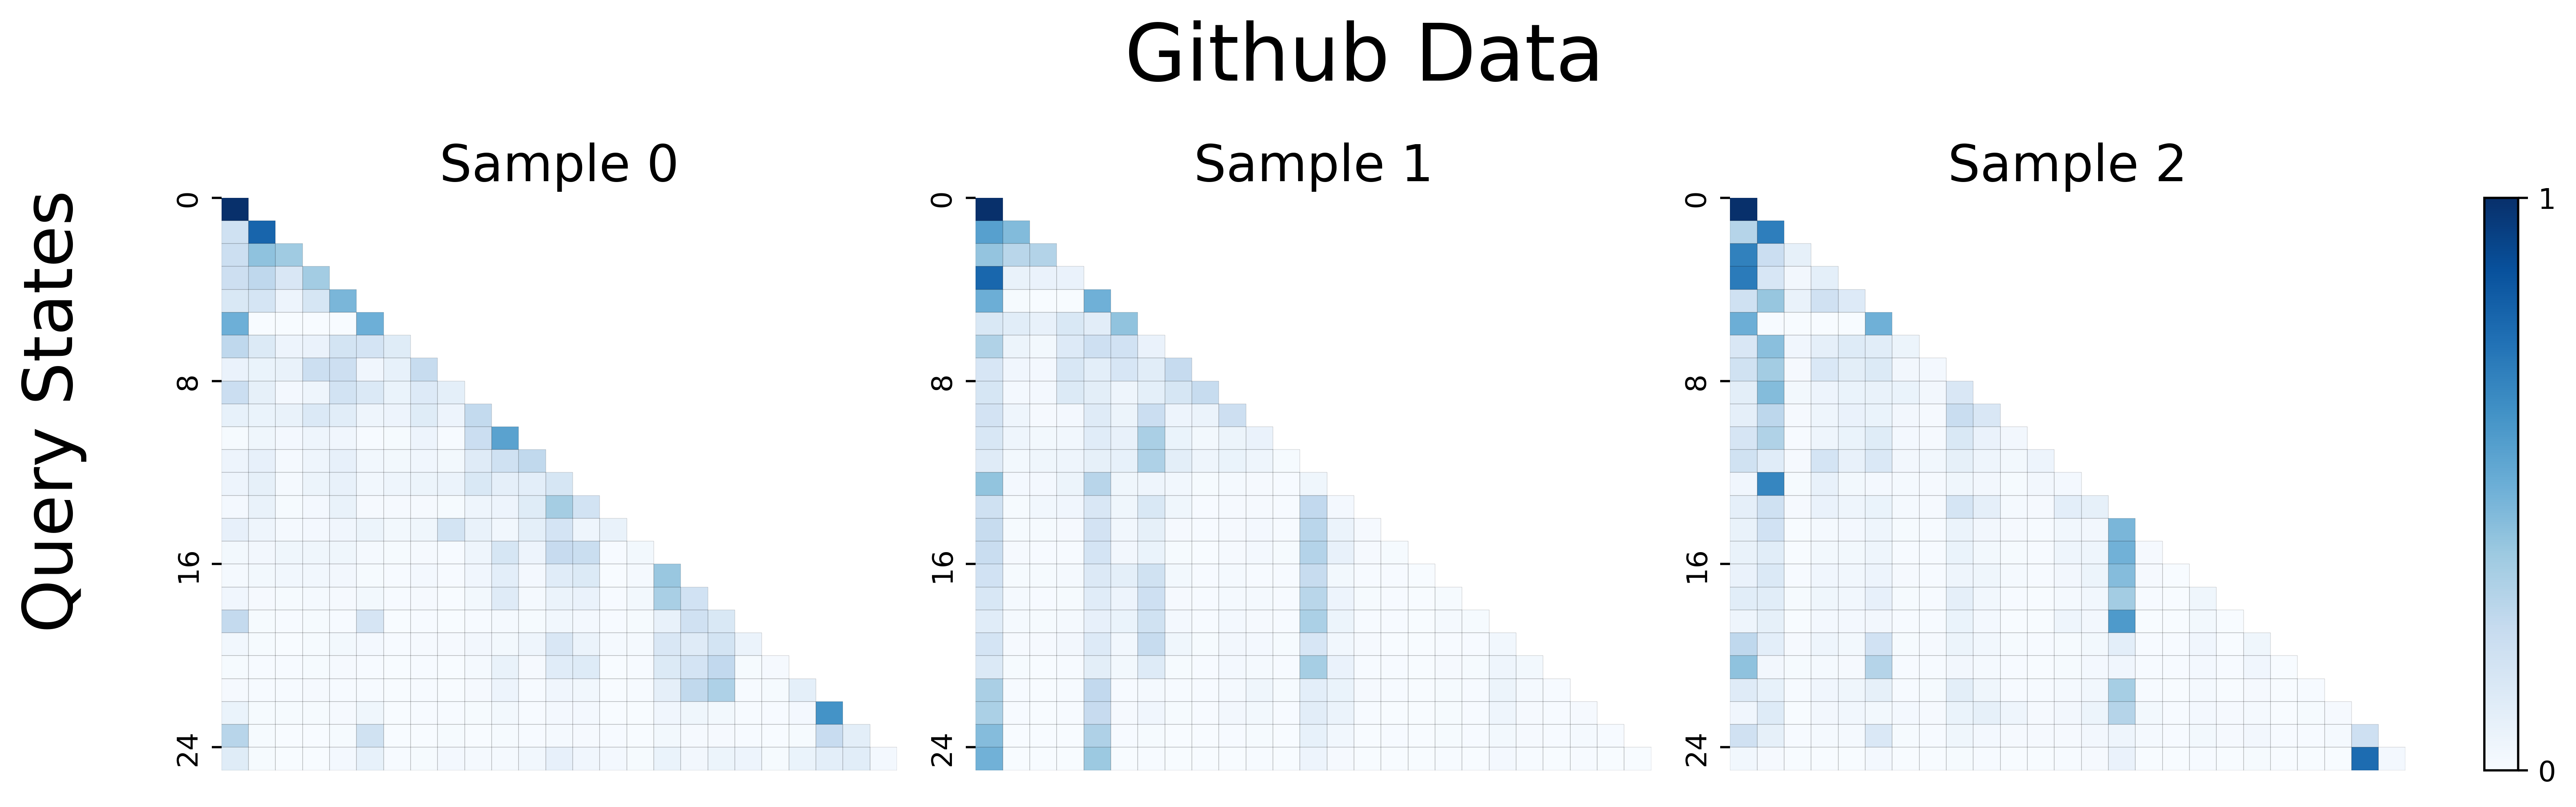
\includegraphics[width=0.9\textwidth]{Figures/L16_H25/attn_github_head25.png}
        
        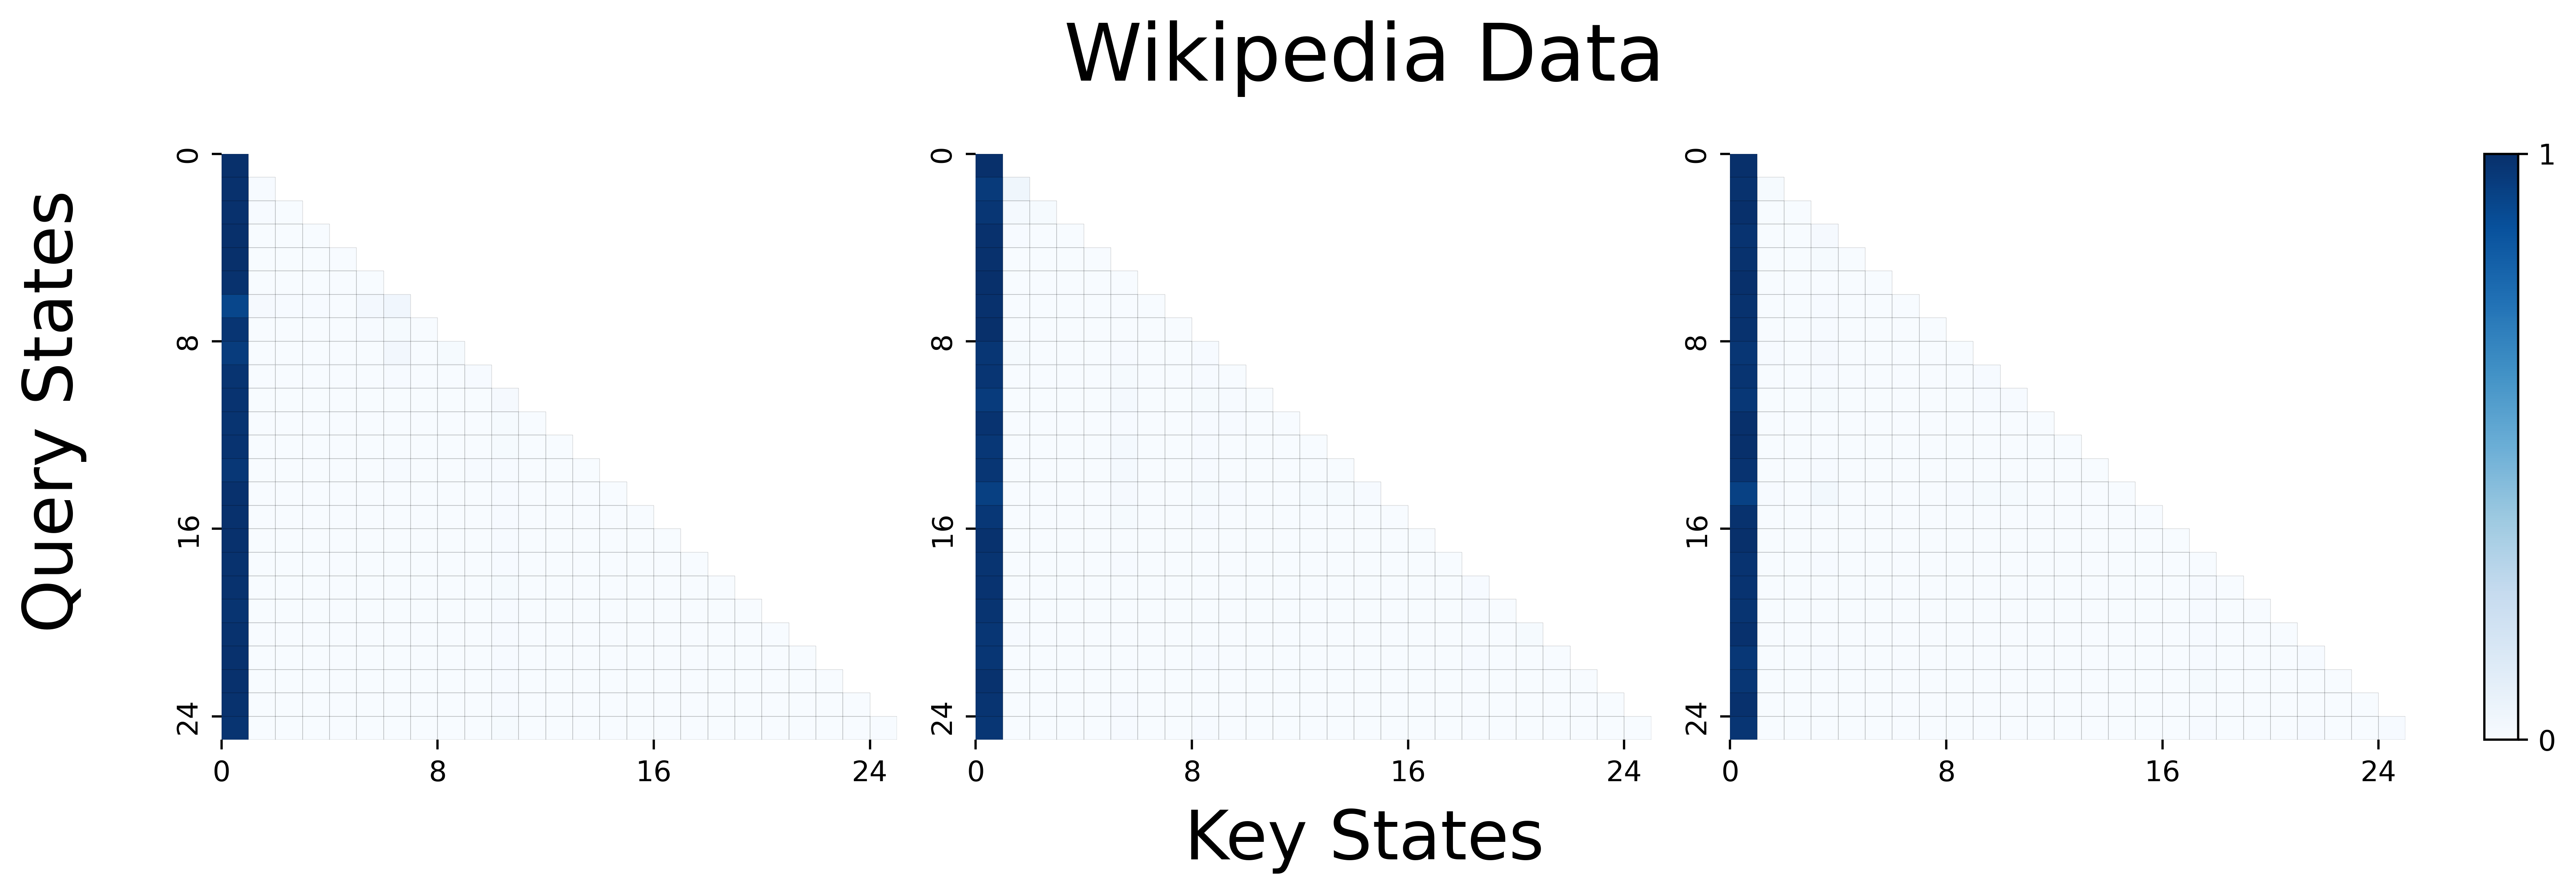
\includegraphics[width=0.9\textwidth]{Figures/L16_H25/attn_wikipedia_head25.png}
        \label{fig:github_wikipedia_weights}
    \end{subfigure}
    \hfill
    \begin{subfigure}[t]{0.38\textwidth}
        \caption{\small Zero-out-head intervention outcomes}
        \label{fig:github_wikipedia_zero_out}
        \vskip1.5em
        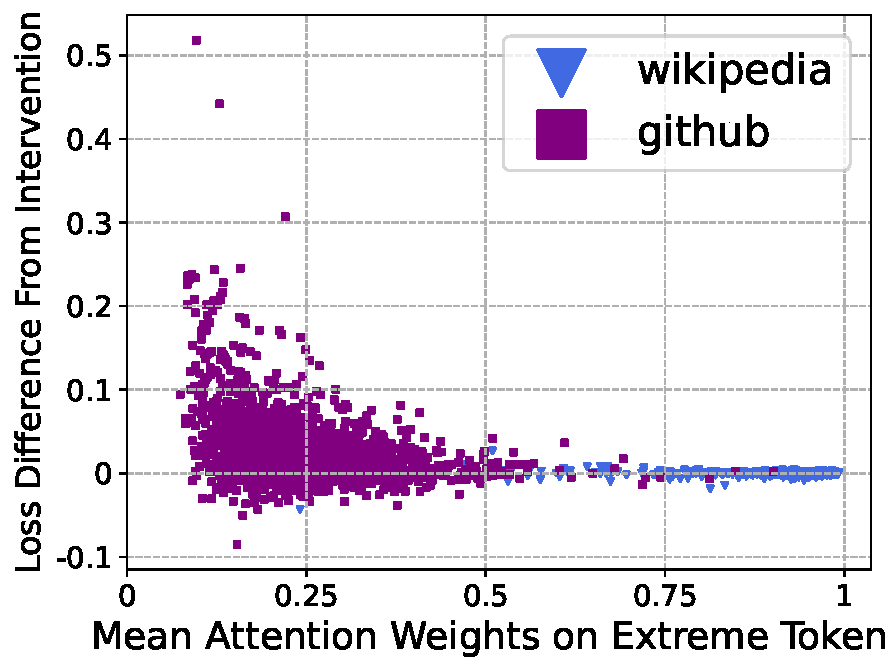
\includegraphics[width=0.9\textwidth]{Figures/BBM/LLM_interventions.pdf}
    \end{subfigure}
    \vspace{-0.5em}
    %\includegraphics[width=0.5\linewidth]{}
    \caption{\small \textbf{Active-dormant mechanism of Layer 16 Head 25 (L16H25) of Llama 2-7B-Base.} We observe that L16H25 is active on GitHub data and dormant on Wikipedia data, both sourced from RedPajama-1T \citep{together2023redpajama}. \textit{Left (a)}: Attention weights of L16H25, prompted by three randomly selected samples from each domain. \textit{Right (b)}: Results of an intervention study showing the change in cross-entropy loss when the output of L16H25 (specifically, its value states) is set to zero across sequences in both domains. The findings indicate that the model's performance for GitHub data, measured by cross-entropy loss, strongly relies on the output of this attention head. 
    % \sm{(a) Truncate at $24$ \sm{right: xlabel and xtick size. $x 0.1$} \sm{High priority} \sm{Orange color change}}
    % heads are sinks in one domain and not others (Llama 2 7B L16H25, GitHub vs Wikipedia) \DP{TODO...}
    % \DP{Plan: two figures. Left: attn sink visualization for GitHub on left and Wikipedia (4x4 (adjust to be visually appealing) samples visualize L16H25). Right: causal intervention, zeroing out head vs cross entropy delta taken across many samples from GitHub and Wikipedia.}
    }
    \label{fig:dormant_heads_domain_dependent}
\end{figure}




    %\textit{If all tokens at a head do not have helpful value states for predicting the next token, then attention mass will concentrate on tokens which are generally unhelpful for next-token prediction (like \bos). \sm{Attention heads are controlled by the active-dormant mechanism; attention sinks and value-state drains are the dormant phases of attention heads. }}

Our study of the BB model leads to the following prediction with respect to the extreme-token phenomena, which we hypothesize also applies to LLMs:  
\begin{center}
    \textit{Attention heads are controlled by an active-dormant mechanism (cf.\ Claim \ref{claim:active-dormant}). The presence of attention sinks and value-state drains indicates that an attention head is in a dormant phase.}
\end{center}

This hypothesis suggests that in LLMs, whether an attention head becomes a sink depends on the context. Specifically, the attention head may become entirely irrelevant for selecting the next tokens in certain contexts or tasks, but not in others. When this irrelevance occurs, the attention head transitions into an attention sink. This hypothesis was confirmed in small transformers and the BB task, as demonstrated in Section~\ref{sec:bb_task}. 



Accordingly, we aim to identify instances of attention heads in pretrained LLMs that exhibit this active-dormant behavior, i.e., heads that are dormant in some domains but active in others. In \Cref{fig:dormant_heads_domain_dependent}, we display a particular attention head---Layer 16 Head 25 (L16H25) of Llama 2-7B-Base \citep{touvron2023llama}---which demonstrates a clear active-dormant distinction across two distinct contexts (e.g., tokens from the GitHub subset versus the Wikipedia subset of RedPajama \citep{together2023redpajama}). While many attention heads show similar context-dependent behavior (see \Cref{sec:more_heads}), we focus on this one because the conditions for its activation are straightforward and interpretable, whereas other heads may have more nuanced criteria. 
% \sm{Can we plot more figures instead of the figures that are GitHub/Wiki}

\Cref{fig:github_wikipedia_weights} shows the attention maps of L16H25 on samples from both the GitHub and Wikipedia subsets of RedPajama. It demonstrates that L16H26 is \textit{dormant} (i.e., an attention sink) on samples from Wikipedia, which resemble prose, and \textit{active} (i.e., not an attention sink) on samples from GitHub, which resemble code. Additionally, \Cref{fig:github_wikipedia_zero_out} compares the loss difference when L16H25 is zeroed out for prompts from both domains. The results show that zeroing out this head significantly decreases model performance on GitHub sequences, while having minimal impact on Wikipedia sequences. This observation also confirms the head behaves as dormant in some contexts and active in others---in some contexts, removing this head has no effect on model performance, while in others, its removal causes significant performance drops.
% We include more detail in \Cref{sec:circuit}.
% , where we extract a circuit for extreme-token phenomena to examine the dormant-active mechanism and its interaction with input token semantics. \sm{Polish} \sm{Mid priority}



% Accordingly, we strive to find instances of heads in pretrained LLMs that satisfy this principle, i.e., which are dormant on some domains and active on others. In \Cref{fig:dormant_heads_domain_dependent}, we show a particular attention head -- Layer 16 Head 25 of Llama 2-7B-Base \citep{touvron2023llama} --- which has an extremely clear active-dormant distinction across two distinct contexts (e.g., tokens from RedPajama \citep{together2023redpajama} drawn from the GitHub subset versus the Wikipedia subset). While there are many such attention heads which are context-dependent --- we provide some in \Cref{sec:more_heads} --- we demonstrate this one because the conditions under which it is active are simple and interpretable, while others have more involved or complex criteria to become active. We observe that this attention head is \textit{dormant} (i.e., an attention sink) on samples from Wikipedia, which more closely resemble prose, and \textit{active} (i.e., not an attention sink) on samples from GitHub, which more closely resemble code. We also observe that this attention head, in general, contributes significantly to the performance of the model on code sequences, but has negligible impact on the performance of the model on prose sequences (\Cref{fig:github_wikipedia_zero_out}). This is a further justification, from a practical perspective, of why this head is sometimes dormant and sometimes active --- in some contexts we can ablate it from the model entirely with no effect, but in other contexts ablating the head leads to huge performance drops. We include more detail in \Cref{sec:circuit}, where we extract a circuit for extreme-token phenomena in order to analyze the dormant-active mechanism and its interaction with the semantics of the input tokens.

%\footnote{Llama 2-7B-Base has two sink tokens (\bos~and one more) in its attention sink heads, while Llama 3.1-8B-Base only has one (\bos). We discuss a potential reason in \Cref{sub:multiple_sinks_discussion}. \sm{Why we put this remark here?}} \sm{Talk about other heads also has dormant and active phase, though not interpretable. Ablation figures in appendix. } \DP{@SM: the first part is already in the paragraph.} \sm{It would be good to link to figures for other heads. } \DP{sure will add to appendix, and comment out this comments when done}

\subsection{Extreme-token phenomena along training dynamics of LLMs}\label{sub:olmo_dynamics}


\begin{figure}[t]
    \centering
    \begin{subfigure}[t]{0.32\textwidth}
        \centering 
        \caption{\small Attention sink dynamics}
        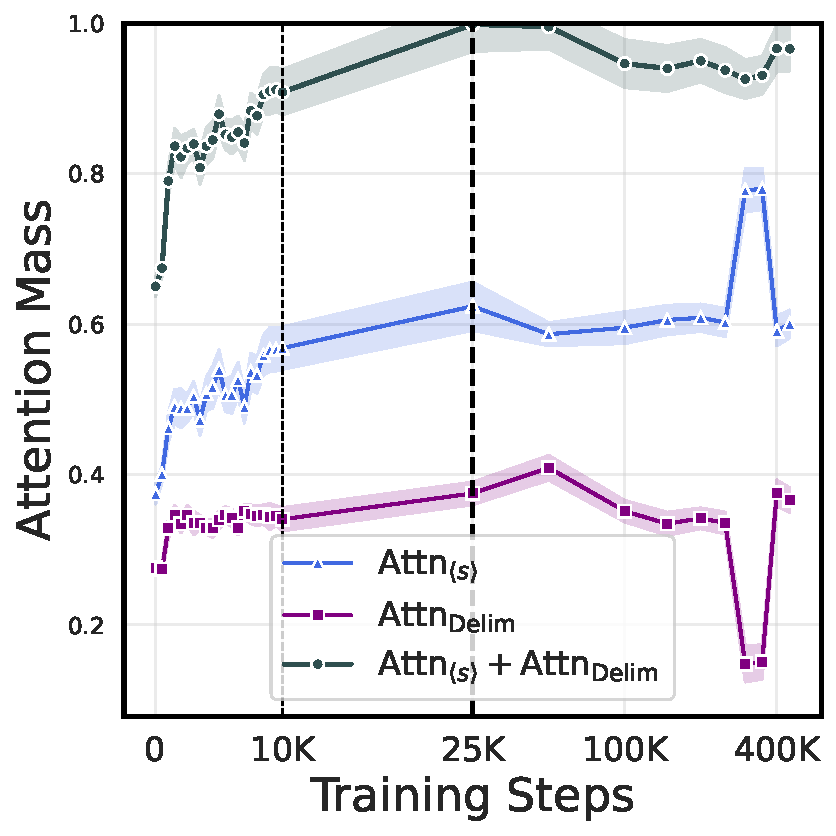
\includegraphics[width=0.9\textwidth]{Figures/olmo/attn_mass_on_top_two_tokens.pdf}
        \label{fig:olmo_sink}
    \end{subfigure}
    \begin{subfigure}[t]{0.32\textwidth}
        \centering 
        \caption{\small Value state dynamics}
        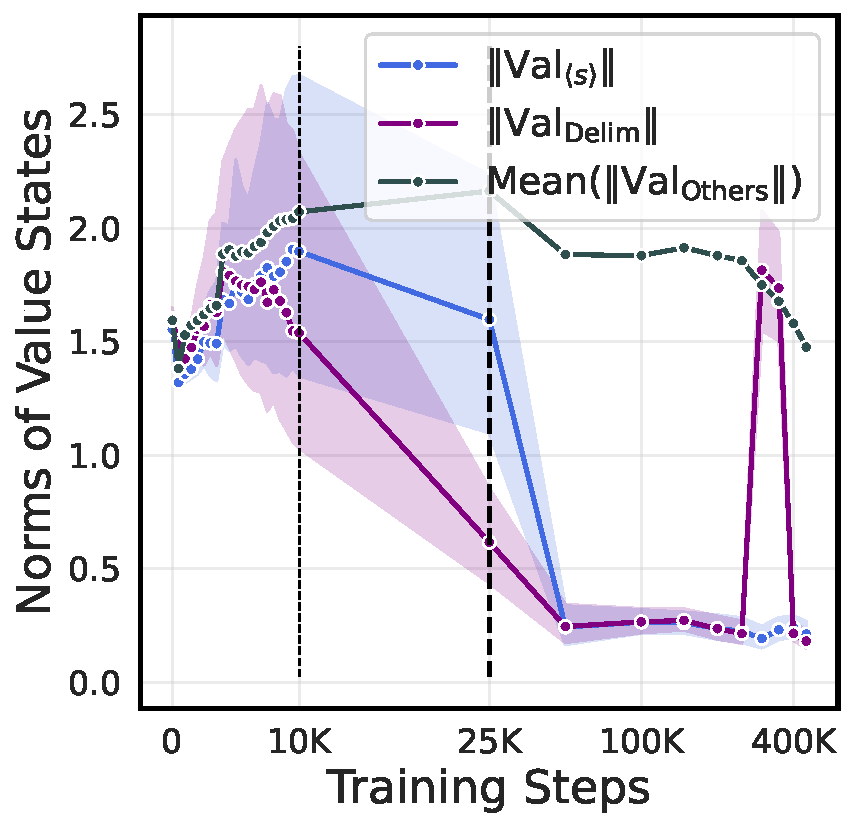
\includegraphics[width=0.9\textwidth]{Figures/olmo/value_norms.pdf}
        \label{fig:olmo_drain}
    \end{subfigure}
    \begin{subfigure}[t]{0.32\textwidth}
        \centering 
        \caption{\small Residual state dynamics}
        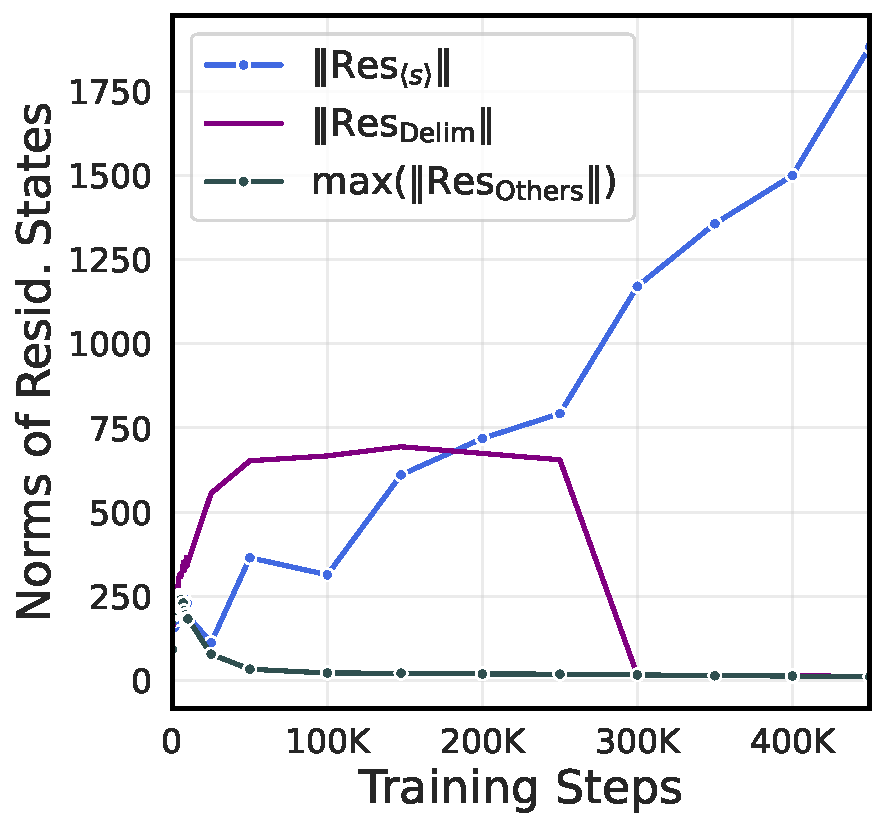
\includegraphics[width=0.9\textwidth]{Figures/olmo/layer_output_norms.pdf}
        \label{fig:olmo_peak}
    \end{subfigure}
    % \vspace{-2em}
    \caption{\small \textbf{Attention weights, value state norms, and residual state norms of Layer 24 during the training dynamics of OLMo.} \textit{Left (a)}: The total attention mass on extreme tokens \bos~and ``\text{Delim}''(\period) at Layer 24, averaged across all attention heads. The horizontal axis is logarithmically scaled after step $10$k. We observe a rapid increase followed by stabilization within the range \([0.9, 1]\) for the rest of training, consistent with our predictions. \textit{Middle (b)}: The value state norms of each token at Layer 24 during training, averaged over all heads. The horizontal axis is logarithmically scaled after step $10k$. Initially, the value states of all tokens shrink, eventually converging, while the value states of the extreme tokens shrink to significantly lower levels compared to other tokens. Figure \textit{(a)} and \textit{(b)} coincide with the trends in Figure~\ref{fig:dynamics} under the BB task. \textit{Right (c)}: The residual state norms of each token at Layer 24 during training. The residual state norm of \bos~increases linearly in magnitude throughout training, matching Figure~\ref{fig:sgd} in the BB task.}
    % \sm{Thicker} \sm{L24 is a bit repetitive} \sm{For (a) and (b), is there a way to draw 0 - 50K using linear scale and 50K - 500K using log scale? This could match better Figure 3(b)} \tianyu{link back to corresponding figures in BB task}}



    
    \label{fig:olmo_predictions_phase0}
\end{figure}
\begin{figure}[h]
    \centering
    \hfill
    \begin{subfigure}[t]{0.32\textwidth}
        \centering 
        \caption{\small Logit dynamics}
        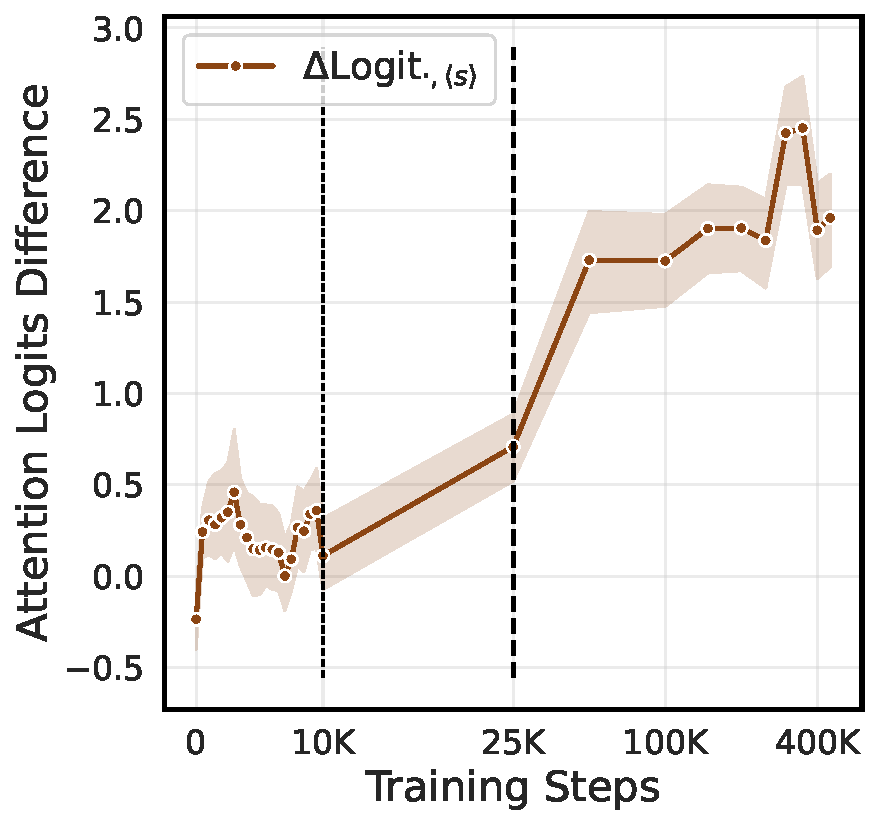
\includegraphics[width=0.9\textwidth]{Figures/olmo/attention_logits.pdf}
        \label{fig:attention_logits_olmo_dynamic}
    \end{subfigure}
    \hfill
    \begin{subfigure}[t]{0.32\textwidth}
        \centering 
        \caption{\small Sink-logits concentration}
        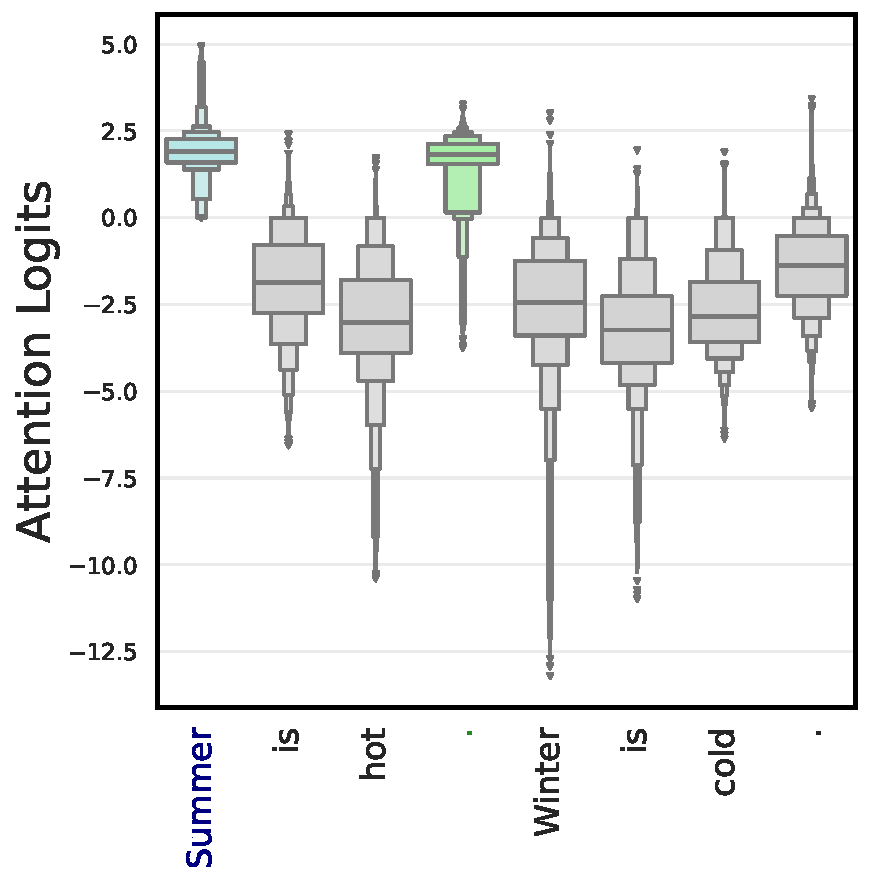
\includegraphics[width=0.9\textwidth]{Figures/olmo/attention_logits_on_test.pdf}
        \label{fig:attention_logits_olmo_static}
    \end{subfigure}
    \hfill
    \phantom{.}
    % \vspace{-2em}
        \caption{\small \textbf{Attention logits of Layer 24.}  \textit{Left (a)}: Attention logits difference of all tokens' query states against \bos's key state during training. The difference in attention logits is computed as \(\Delta\mathrm{logit}_{\cdot,\bos} = \query_{\cdot}^\top \key_{\bos} - \text{Mean}[\query_{\cdot}^\top \key_{\text{Others}}]\). The horizontal axis is logarithmically scaled after step $10k$. We observe that $\Delta \mathrm{logit}_{\cdot,\bos}$ increases approximately in logarithmic scale during training steps $10$k to $100$k, matching the decreasing phase of the value states in Figure~\ref{fig:olmo_drain}. 
        % This behavior aligns with the stable-phase prediction made in the BB model in \Cref{thm:main}(c). Note that this prediction does not apply to the logit corresponding to the zeroth query and key token, as its softmax value will be set to \(1\), making its behavior irrelevant for prediction. 
        \textit{Right (b)}: Attention logits of the last token's query state against all token's key states for pretrained OLMo. In this experiment, we generate \(128\) randomly sampled test tokens with IDs from \(100\) to \(50000\) in the OLMo tokenizer. We append each token separately to the test phrase ``Summer is warm\period~Winter is cold\period'', creating \(128\) different samples, which we feed to the LLM to examine the model behavior. We plot the distribution of (un-shifted) attention logits \( \text{logit}_{\cdot,\tok}=\query_{\mathrm{test}}^\top \key_{\tok}\) across all heads at Layer 24 and all test tokens. The distribution of $\text{logit}_{\cdot,\bos}$ and $\text{logit}_{\cdot,\text{Delim}}$ have considerably small variance compared with other logits, confirming the sink-logits concentration phenomenon. }
        % \tianyu{maybe to make it more clear, we can say that the variance of the attention logits on \bos~is small. Or we can use a new name (attention logits concentration)} \sm{tick size. Box thicker. } \sm{pdf} \tianyu{change the logit in (a)}}
    % \caption{\small \textbf{Attention logits of Layer 24.}  \textit{Left (a)}: The normalized attention logits of all tokens' query states against \bos's key state during training \sm{Is it the opposite?}. We observe that the logits of all non-extreme tokens' query states against \bos's key state in OLMo's Layer 24 are stable for a large fraction of the training run, after an initialization period. This echoes the stable phase prediction made in the BB model in \Cref{thm:main}(c). Note that this prediction makes no guarantees about the logit corresponding to the zeroth query token and zeroth key token, which will be set to \(1\) by the softmax and so its behavior is irrelevant for prediction. Also note that we use normalization, similar to \Cref{sec:bb_task}, to make all terms comparable; namely we have \(\mathrm{logit}_{i} = \langle \query_{i}, \key_{0}\rangle - \mathtt{mean}_{j}(\langle \query_{i}, \key_{j}\rangle)\). \textit{Right (b)}: \sm{A summary phrase of the figure.} For this experiment, we generate \(128\) randomly sampled test tokens with IDs from \(100\) to \(50000\) in the OLMo tokenizer. We append each token separately to the test phrase ``Summer is warm. Winter is cold.'', creating \(128\) different samples, which we feed to the LLM to record the model behavior. We plot the distribution of (un-normalized) dot products \(\langle \query_{\mathrm{test}}, \key_{j}\rangle\) across all heads at Layer 24 and all test tokens. We observe that logits of all regular tokens have very similar distributions, and the distributions of the logits corresponding to extreme tokens \(0\) and \(3\) are also similar. \sm{Why similar? } This confirms the hypothesis that at the end of training, attention heads converge to the stable phase, with similar logits on extreme tokens. \tianyu{maybe to make it more clear, we can say that the variance of the attention logits on \bos~is small. Or we can use a new name (attention logits concentration)} \sm{tick size. Box thicker. } }
    \label{fig:olmo_predictions_phase1}
\end{figure}


Our study of the BB model leads to the following prediction about the dynamical behavior of the extreme-token phenomena, which we hypothesize also applies to LLMs:  
\begin{center}
    \textit{Attention heads undergo an attention-increasing and value-state-shrinking phase driven by the mutual reinforcement mechanism (cf.\ Claim~\ref{claim:mutual-reinforcement}). This is followed by a stable phase, where all non-trigger tokens have large, nearly identical attention logits on the extreme token. Simultaneously, the residual state norms of the extreme tokens increase linearly during pretraining.}
\end{center}



% We confirm these predictions below, thus demonstrating the overall validity of the BB task as a model for extreme token phenomena in LLMs. 
We confirm these predictions below. To observe the training dynamics of a large-scale LLM, we use the setup of OLMo-7B-0424 \citep{groeneveld2024olmo} (henceforth just referred to as OLMo), which provides open-sourced weights at various stages of their training.\footnote{We did not analyze Llama for dynamics, as they do not provide open-source intermediate checkpoints along pretraining.} For our analysis, we inspect OLMo at multiple checkpoints: every 500 steps for the first 10,000 steps, then at 25,000 steps, 50,000 steps, and every 50,000 steps up to 449,000 steps (approximately the end of their training).\footnote{For the single 150,000-step checkpoint, we observed that its statistics were outliers, which we hypothesize is due to a system failure. We address this by using the average of nearby checkpoints to represent its statistics.} The input we use for this analysis is again ``Summer is warm\period~Winter is cold\period''\footnote{Note that OLMo does not have a \bos~token, but attention sinks still form in the majority of heads. In particular, the first token always behaves as an attention sink. We discuss this further in \Cref{sub:fixed_bos}.} In this prompt, the ``$\mathrm{Delim}$'' token, namely ``\period'', also becomes a sink token along with \bos. We believe this occurs because the period is not semantically meaningful and is not useful for predicting future tokens (cf.\  \Cref{sub:fixed_bos}) 
% \sm{Footnote 4 could be made as part of the main text}


% \tianyu{revise the mutual reinforcement mech part}
\Cref{fig:olmo_predictions_phase0} illustrates the dynamics of attention weights, value state norms, and the residual state norms for attention heads in Layer 24 of OLMo. The figure shows that the average attention on extreme tokens (\bos~and $\mathrm{Delim}$) increases rapidly at the beginning of training before stablizing, while the value state norms of these extreme tokens decrease during training steps 10k-100k. The synchronized evolution of attention weights and value state norms aligns with the prediction of the mutual reinforcement mechanism.  Additionally, the residual states of \bos~increase linearly, while those of other tokens converge to a small number. \Cref{fig:olmo_predictions_phase1} provides a more detailed examination of the attention logits in Layer 24 of OLMo. Figure~\ref{fig:attention_logits_olmo_dynamic} presents the dynamics of the difference in attention logits, showing that $\Delta \text{logit}_{\cdot,\bos}$ increase during training steps 10k-100k, matching the decreasing phase of the value states.
Figure~\ref{fig:attention_logits_olmo_static} also demonstrates the \textit{sink-logits concentration} phenomenon. Specifically, it shows that the sink logits will eventually converge to a stable phase, in which logits corresponding to the key of the sink token and queries of all non-sink tokens are nearly identical. These findings coincide with the dynamical behavior predicted by the BB model, as outlined in Theorem~\ref{thm:main}(c) and corroborated by the experimental results in \Cref{figure:verify-assumptions}. 

% with the attention logits corresponding to \bos's key and other token's query converging to near identical value \sm{Name for this logit}
% In \Cref{fig:olmo_predictions_phase0}, we confirm that attention heads go through an attention-increasing and value-state-shrinking phase, and that the residual state norm of the \bos{} token increases linearly during pretraining. We show that, at Layer 24 of OLMo, the average attention on extreme tokens (\bos~and $\mathrm{Delim}$) increases rapidly at the beginning of training and converges to a constant, while the value state norms of extreme tokens decrease rapidly. Also, the residual states of extreme tokens also increase linearly, while the rest quickly converge. In \Cref{fig:olmo_predictions_phase1} we show that attention heads converge to a stable phase, and that all logits corresponding to the first token's value states (i.e., all tokens' value of \(\mathrm{logit}_{0}\), except possibly the value of \(\mathrm{logit}_{0}\) corresponding to \bos~itself) have similar distributions. These confirm our dynamics insights from the BB model (cf.\ \Cref{figure:verify-assumptions}). 

%\sm{These echos the findings from the BB model. Link figure 3b here. }
% Outline:
% \begin{itemize}
%     \item OLMo value states at a middle layer are roughly constant over time except for bos token and first delimiter
%     \item Massive norm keeps increasing over time 
%     \item Attention sink occurs very rapidly and stays constant over time
% \end{itemize}

% \begin{figure}
%     \centering
%     %\includegraphics[width=0.5\linewidth]{}
%     \caption{Training dynamics of value states, massive norm, and attention sink via OLMo
%     \DP{TODO: for attention logits plot, put linear plot for first 10k epochs (halfway through axis) and log plot for remaining epochs; do the same for value states; plot multiple heads for value plot}}
%     \label{fig:enter-label}
% \end{figure}













% \section{Case Study and Motivation}\label{sec:case_study}

In this section, we will study a particular attention head in Llama 2, and use its behavior as a motivation for the more general analysis that follows.

\subsection{Preliminaries}\label{sub:prelim}

\DP{TODO @TG: Fill out a simplified notation block. Please ensure that the simplified notation is consistent with the notation in the appendix.}

\DP{TODO: mention that we pre-pend all inputs with \bos.}

A significantly more precise setup and notation is detailed in \Cref{sub:app_notation}.

\subsection{Understanding Layer 16 Attention Head 25 of Llama 2}\label{sub:case_study_l25_h16}

As motivation for our later reasoning, we will now examine the behavior of Layer 16 Attention Head 25 (abbreviated as L16H25) in Llama 2 7B, on both prose from the Wikipedia dataset \citep{wikidump} and code from the RedPajama Github dataset \citep{together2023redpajama}. This is the first attention head which we identify as a dormant head, and we want to understand its properties at a more fine-grained level. First, let us examine the difference in perplexity on samples of these two datasets obtained from the full forward pass versus a modified forward pass where the output of the attention head L16H25 is zeroed out. Specifically, we evaluate each forward pass on 32 samples of their respective datasets, where each sample is truncated to 64 tokens. We observe the results in \Cref{tab:ppl_wiki_github_l16h25}. Overall, the performance change is greater on the GitHub data than on the Wikipedia data, which signals that it may be the case that L16H25 is function-less on the Wikipedia data yet has a function on the GitHub data. To confirm our hypothesis, we plot the (post-softmax) attention weights on a few representative samples of GitHub and Wikipedia data in \Cref{fig:attn_l16_h25_small} (and \Cref{fig:attn_l16_h25_improved} in \Cref{sub:app_supporting_lots_of_heads}). We observe that L16H25 is an attention sink \citep{xiao2023efficient} on Wikipedia data. This means that for each sample, the attention head outputs roughly the same vector (or one of a few possible vectors) for each token position, acting like a bias which does not use correlations between tokens. On the other hand, on GitHub data L16H25 is not an attention sink. This discrepancy motivates the definition of a dormant head, expanded on in \Cref{sec:dormant_heads}, that a dormant head is one which does not use correlations between tokens to obtain an output (and thus is not impacted by the semantics of the input). To confirm this, we also plot the pre-softmax logits in \Cref{fig:attn_logits_l16_h25_small} (and \Cref{fig:attn_logits_l16_h25_improved} in \Cref{sub:app_supporting_lots_of_heads}). \DP{TODO: @TG could you give some reasoning here?}

\begin{table}
    \centering
    \caption{\small \textbf{Perplexity of Llama 2 7B when using an unmodified forward pass vs.~a forward pass which is modified to set the output of L16H25 to \(0\).} We observe that while the perplexity does not change substantially on Wikipedia data, it noticeably increases on Github data. This motivates the hypothesis that L16H25 is ``dormant'' for Wikipedia data and ``active'' for Wikipedia data.}
    \begin{tabular}{@{}lll@{}}
    \toprule
    \textbf{Perplexity}    & Wikipedia Dataset & Github Dataset \\ \midrule
    Unmodified forward pass                  &                   &                \\
    Modified forward pass  &                   &                \\ \bottomrule
    \end{tabular} 
    \label{tab:ppl_wiki_github_l16h25}
\end{table}

\begin{figure}
    \centering
    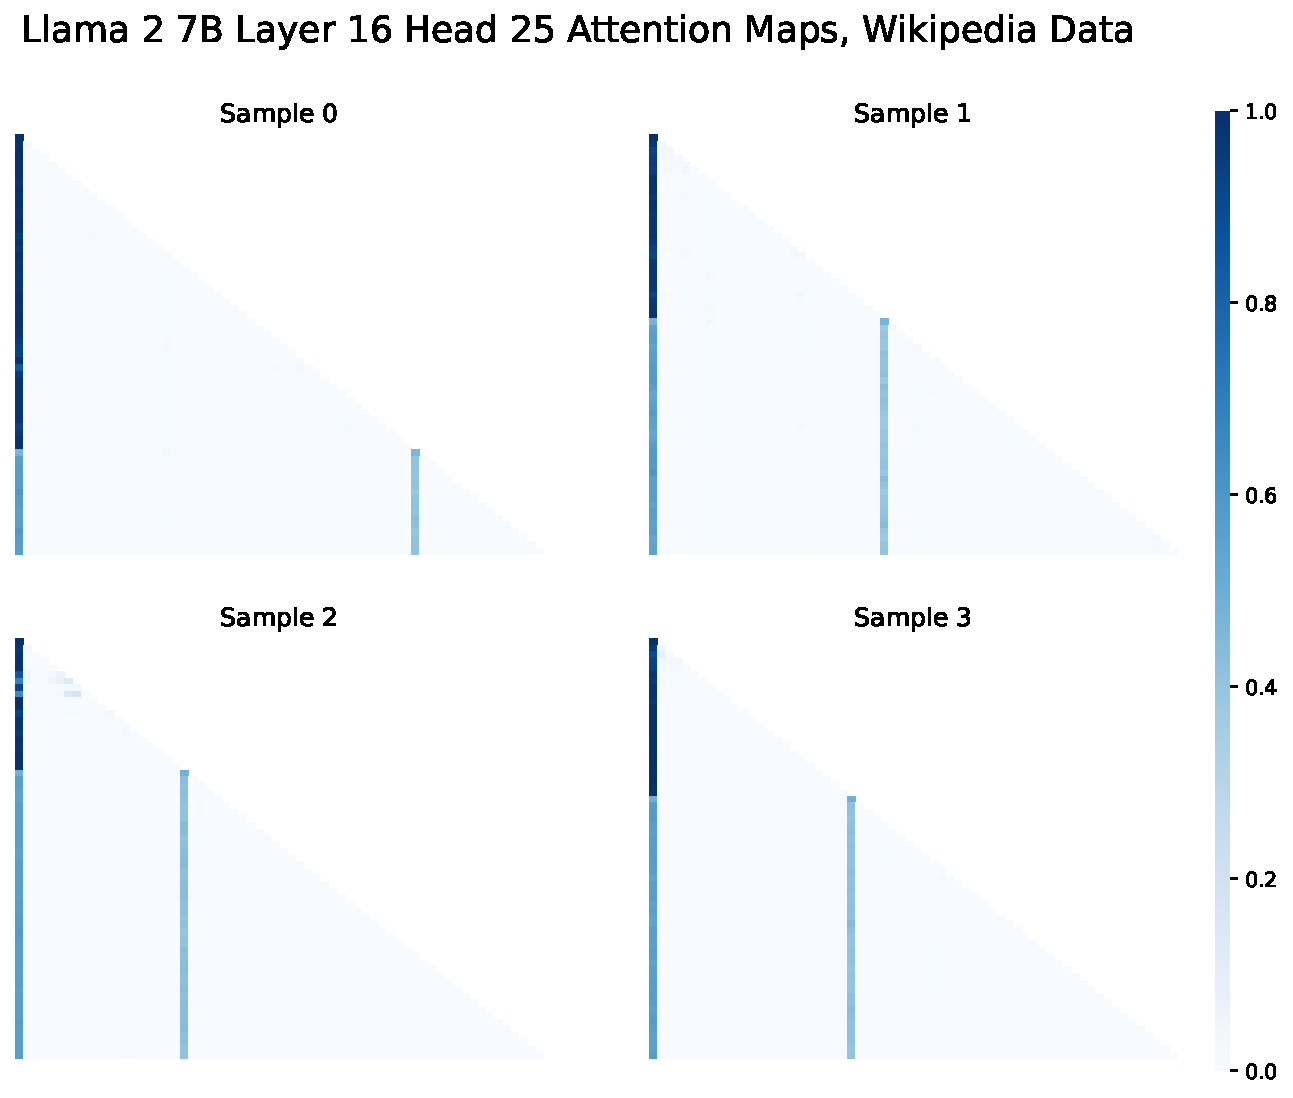
\includegraphics[width=0.45\textwidth]{Figures/L16_H25/attn_maps_l16h25_wiki_small.pdf}
    \hspace{0.075\textwidth}
    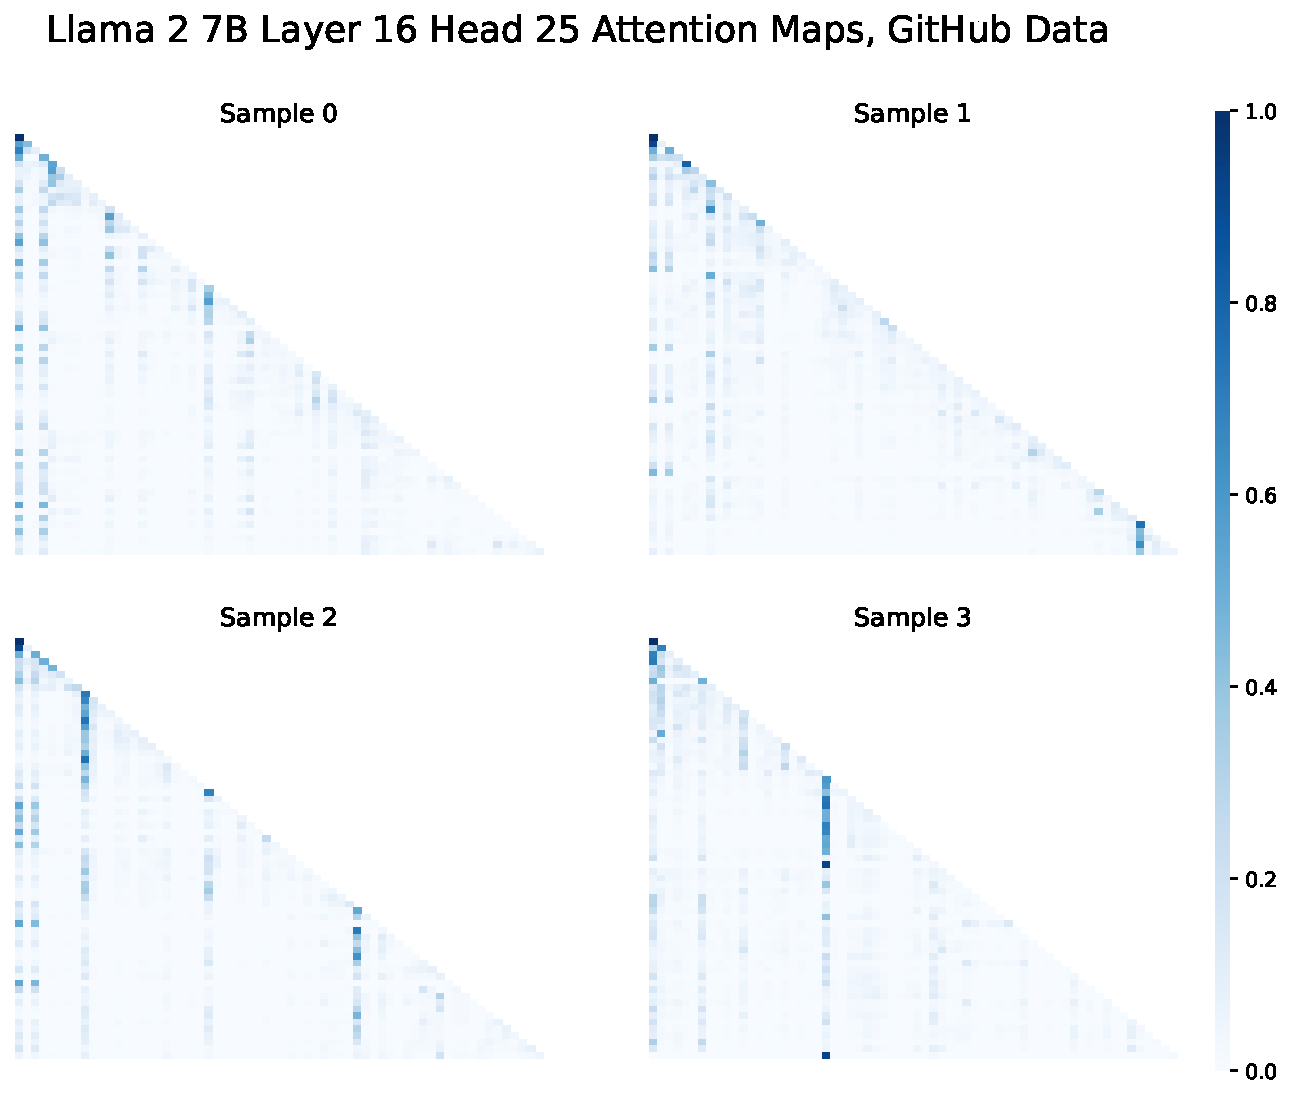
\includegraphics[width=0.45\textwidth]{Figures/L16_H25/attn_maps_l16h25_github_small.pdf}
    \caption{\small\textbf{Visualizations of attention weights for Llama 2 7B L16H25 on both Wikipedia and GitHub data.} On four random samples from each domain, we truncate each sample to 64 tokens and visualize the (post-softmax) attention weights from this head. We observe that for Wikipedia the head has one or two attention sinks, while for GitHub the head has no attention sink, corresponding to our hypothesis that the head is ``dormant'' on Wikipedia and ``active'' on GitHub. Further samples are plotted in \Cref{fig:attn_l16_h25_improved}, maintaining this trend.}
    \label{fig:attn_l16_h25_small}
\end{figure}


\begin{figure}
    \centering
    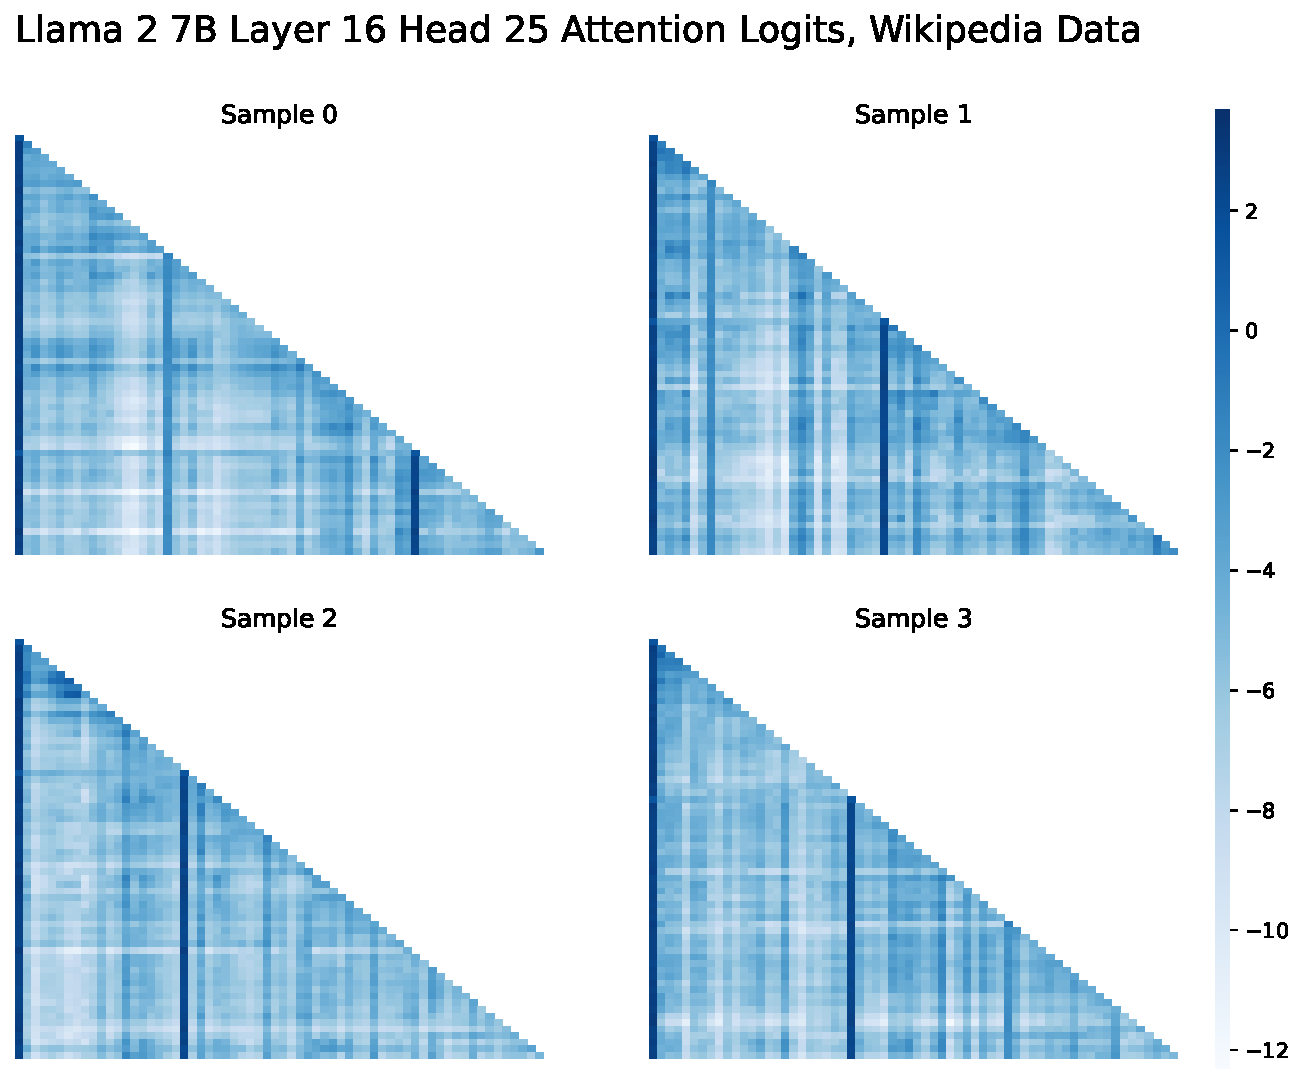
\includegraphics[width=0.45\textwidth]{Figures/L16_H25/attn_logits_l16h25_wiki_small.pdf}
    \hspace{0.075\textwidth}
    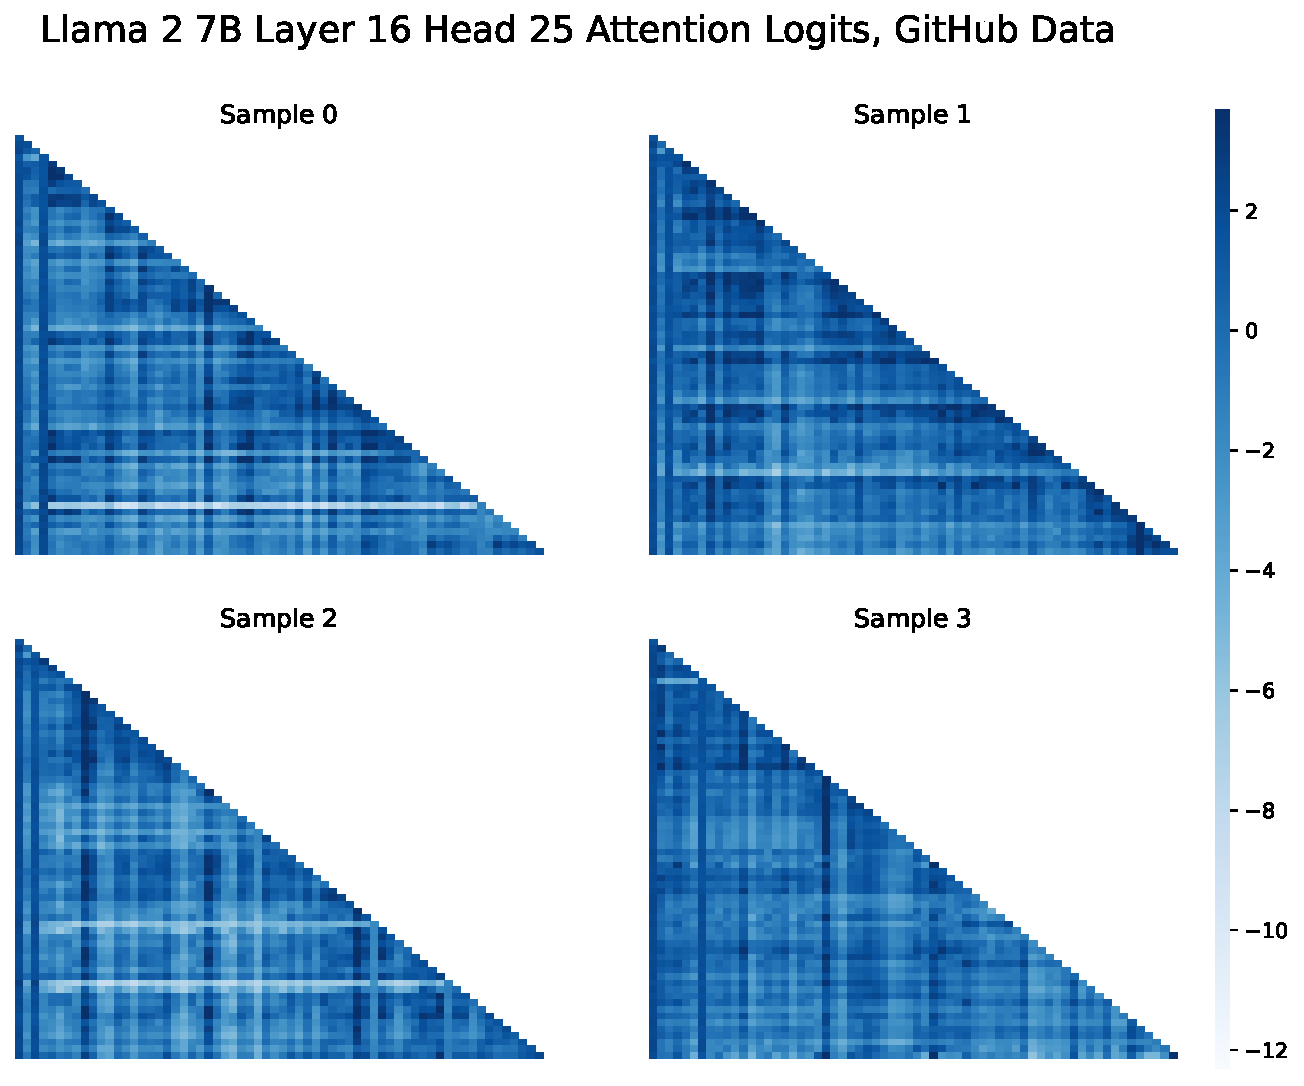
\includegraphics[width=0.45\textwidth]{Figures/L16_H25/attn_logits_l16h25_github_small.pdf}
    \caption{\small\textbf{Visualizations of pre-softmax attention logits for Llama 2 7B L16H25 on both Wikipedia and GitHub data.} \DP{@TG: please fill in the description here and in main body.} Further samples are plotted in \Cref{fig:attn_logits_l16_h25_improved}, maintaining this trend. \tianyu{how about deleting this figure? It's hard to tell that the logits are around the same. Instead, how about make annotations on previous figure, showing the attention logits on bos?}}
    \label{fig:attn_logits_l16_h25_small}
\end{figure}


% \section{Dormant Attention Heads}\label{sec:dormant_heads}
 
 In this section, we will more carefully define dormant heads and show that they are ubiquitous on both pre-trained LLMs and small transformers trained via next-token-prediction.

\subsection{Dormant Head Conjecture} \label{sub:dormant_head_conjecture}

As in \Cref{sub:case_study_l25_h16}, we define a \textit{dormant attention head} as follows.
\begin{quote}
    \textit{An attention head is \underline{dormant} on a particular input if its output consists of only one (or a small number of) vector(s), repeated across every token index.}
\end{quote}
 The output of a dormant head does not respect the semantic content of the input, and essentially outputs a bias. Heads which are attention sinks are dormant attention heads, and indeed almost all (but not necessarily all) dormant attention heads are attention sinks. Our \textit{dormant heads conjecture} states that dormant heads are ubiquitous in LLMs. In particular, we say that a head which is not dormant is \textit{active}. Then, we conjecture the following:
 \begin{quote}
     \textit{\underline{Dormant heads conjecture:} for autoregressive transformer-based language models, a large fraction of heads are dormant on some inputs and active on some others.}
 \end{quote}
 In this section, we will provide evidence for this conjecture through finding a circuit in Llama 2 7B which creates dormant heads (\Cref{sub:circuit_evidence}), developing an automated detection system for attention sinks and thus showing that many heads in Llama 2 7B are empirically dormant on some inputs and active on others (\Cref{sub:lots_of_dormant_heads}), and showing that the dormant head phenomenon persists in small autoregressive transformers trained on next-token-prediction (\Cref{sub:controlled_experiments}).

\DP{TODO: description}

\subsection{Evidence 1 For Conjecture: Circuit for Dormant Heads in Llama 2} \label{sub:circuit_evidence}

\DP{TODO: description}

\begin{figure}[t]
  \centering
  % \begin{minipage}{0.24\textwidth}
  %     \centering
  %     \subcaption{\small Attention weights}
  %     \label{fig:circuit-attn-weights}
  %     \vspace{-.2em}
  %     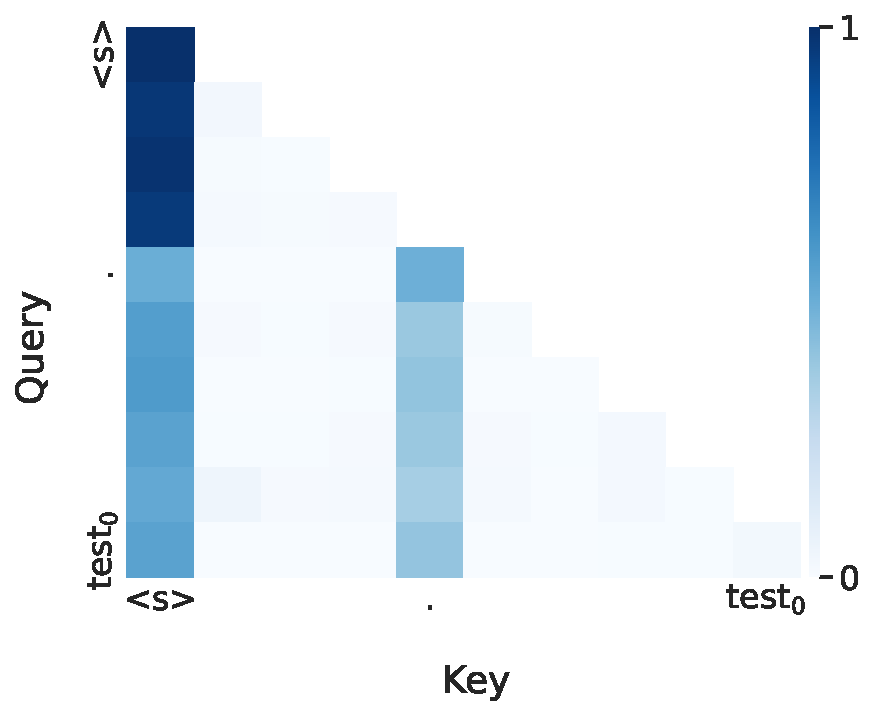
\includegraphics[width=\linewidth]{Figures/figures_circuit/attn_weights_dormant.pdf}
  % \end{minipage}
  % \hspace{-1em}
  \begin{minipage}{0.33\textwidth}
      \centering
      \subcaption{\small Attention logits}
      \label{fig:circuit-attn-logits}
      \vspace{-.2em}
      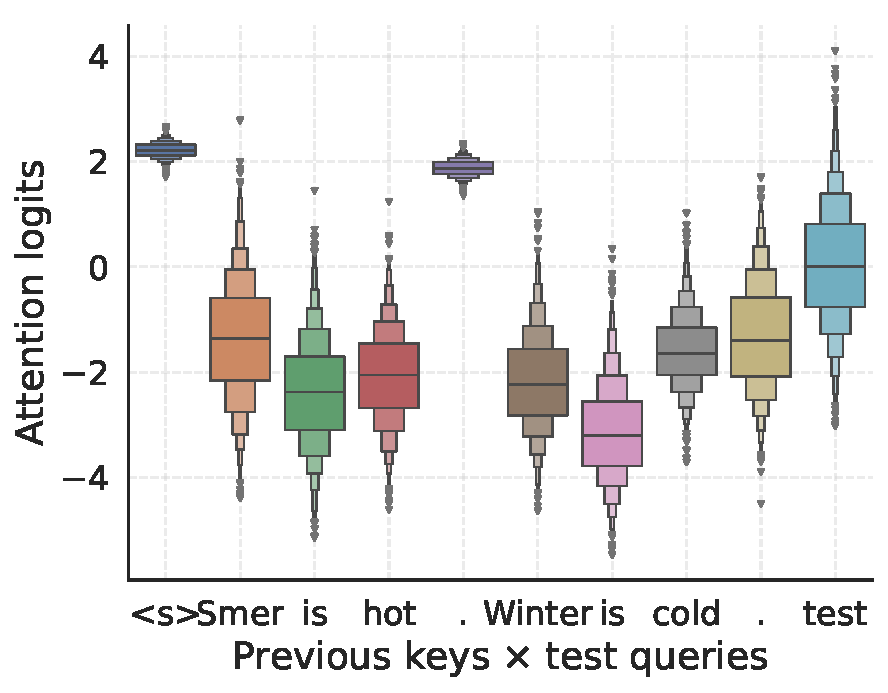
\includegraphics[width=\linewidth]{Figures/figures_circuit/logits.pdf}
  \end{minipage}~
  % \hspace{-1em}
  \begin{minipage}{0.33\textwidth}
      \centering
      \subcaption{\small Output norm}
      \label{fig:circuit-massive-norm}
      \vspace{-.2em}
      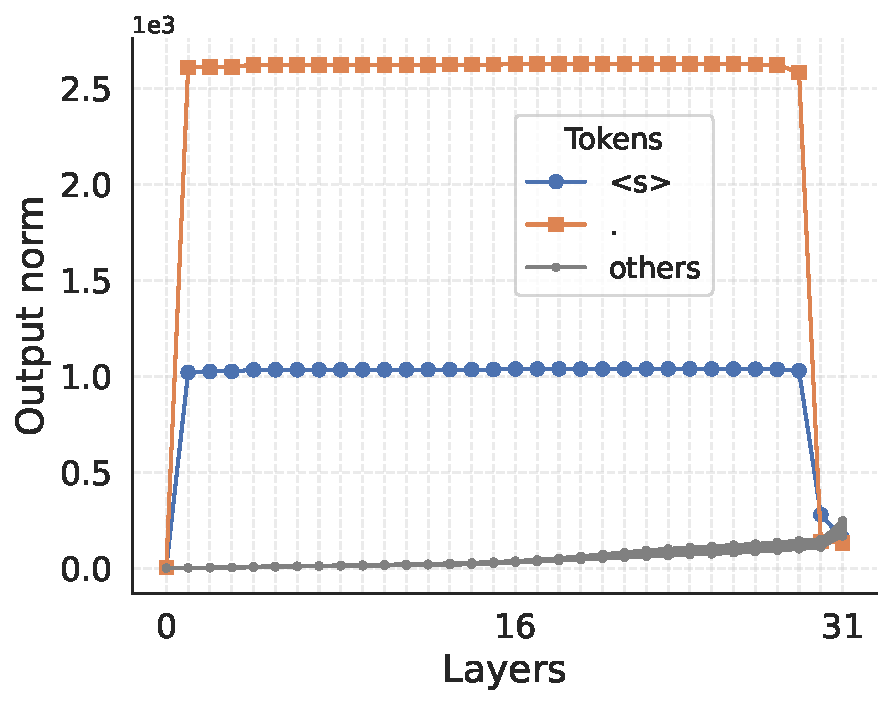
\includegraphics[width=\linewidth]{Figures/figures_circuit/massive.pdf}
  \end{minipage}
  \hspace{-1em}
  \begin{minipage}{0.33\textwidth}
      \centering
      \subcaption{\small Value states norm}
      \label{fig:circuit-value-norm}
      \vspace{-.2em}
      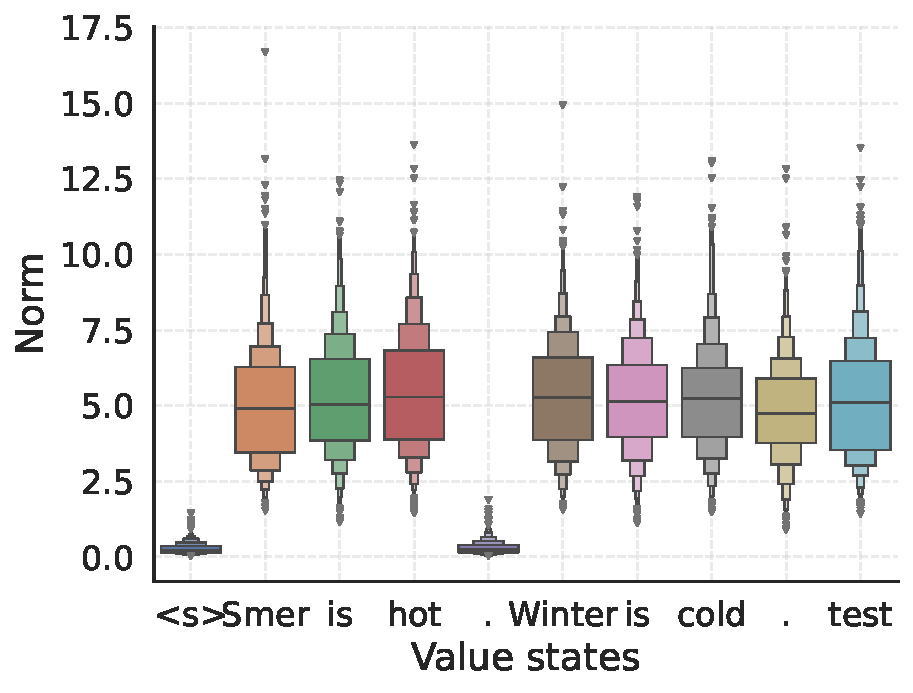
\includegraphics[width=\linewidth]{Figures/figures_circuit/values.pdf}
  \end{minipage}
  \vspace{-1em}
  \caption{\small \textit{Algebraic findings.} We sample ``\bos~Summer is hot. Winter is cold.'' $+$ ``random test token'''s for $1000$ times to obtain a distribution of hidden states in \llama. Figure \ref{fig:circuit-attn-logits} presents the attention logits computed by using the test tokens as queries and the previous tokens as keys. The logits on \bos~and the first \delim are effectively positive constants, with logits on other tokens vary among different test tokens, and being mostly negative. Figure \ref{fig:circuit-massive-norm} shows the norm of the outputs across all the layers, with the \bos~and the first \delim possessing significantly massive norms from layers 2 to 29. Figure \ref{fig:circuit-value-norm} shows the norm distribution of the value states across layers 2 to 29. The norms of the \bos~and the first \delim token are effectively small constants. 
  }
  \label{figure:algebra-findings}
  \vspace{-1em}
\end{figure}



We summarize the algebraic features of \bos~ and the first \delim tokens in the computation graph, all of which point to the dormant heads conjecture. Previous works discover parts of these features separately. As a demonstration, we randomly sample 1000 tokens from the vocabulary of \llama, prefix it with ``\bos~Summer is hot. Winter is cold.'' to form one test sequence, and implement the forward pass. By collecting  hidden states for each test sequence, it provides us with a distribution of hidden states.
\ref{figure:algebra-findings} summarizes the four algebraic features:
\begin{enumerate}
    \item \textit{Attention sink}: Figure XXX visualizes the attention weights. Before the first \delim, the attention weights from all tokens on \bos~are near 1. The \delim would split half of the attention weights on \bos.
    \item \textit{Stable attention logits}: Figure \ref{fig:circuit-attn-logits} presents the attention logits from the test token (query) on tokens in the prefix (key). The distribution comes from a fixed head, L16H25, with 1000 test tokens. The attention logits on \bos~and \delim are nearly constant across all test tokens, while vary a lot on other tokens. 
    \item \textit{Massive norms}: Figure \ref{fig:circuit-massive-norm} presents the norm of hidden states across layer 0 to 31, averaged among 1000 test sequences. The \bos~and \delim have norms around 500 to 1000 times of other tokens.
    \item \textit{Small value states}: Figure \ref{fig:circuit-value-norm} shows the norm distribution of norms of value states. The distribution comes from all heads from layer 2 to 29 and with 1000 test tokens. \bos~and the first \delim both possess negligible norm.
\end{enumerate}

\tianyu{I will postpone the circuit here}
The algebraic findings depict a potential circuit of the dormant mechanism. Figure XXX illustrates the entire procedure, which we summarize as follows:
\begin{enumerate}
    \item Preparatory phase (layer 0 and 1): The $\mlp$ of layer 1 adds an output with massive norm residual streams of \bos~and the first \delim tokens. Using causal ablations, we verify the function of each components in layer 0 and 1.
    \begin{enumerate}
        \item \tianyu{We need to discuss the names here} Both the $\MLP$ in layer 0 and 1 contribute to the formation of a XXX in layer 1.
        \item $\Attn$ in both layer 0 and 1 adjust the formation of XXX. For example, shown by zero-out intervention, L1H8 both assists the initial token to be XXX and suppresses the other tokens to be XXX.
        \item The \rope in $\Attn$ heads in layer 0 and 1 suppresses the formation of XXX starting from the second delimiter tokens.
    \end{enumerate}
    \item Dormant/active phase: At this stage, the residual streams of \bos~and the first \delim remain nearly untouched, since any outputs added on the residual stream have negligible norms. At the main time, the layer norm map them to a special direction XXX, which corresponds to a sink key state which has nearly constant attention logits fitted with any queries. The direction XXX also possesses minor value states,. As a result, a test token has two modes on the attention weights:
    \begin{itemize}
        \item dormant mode: when no other keys align with its queries. After the Softmax function, \bos~and the first \delim take up a great proportion of its attention weights
        \item active mode: when there's other key that aligns with its query, which renders a attention logits comparable or even greater than the attention logits on \bos. After the Softmax function, \bos~and the first \delim take up a small proportion of its attention weights.
    \end{itemize}
    Since the value states of \bos~and \delim are notably small,
    The different modes on attention weights lead to different     \begin{itemize}
        \item dormant mode: add a minor output on the residual stream
        \item active mode: add a large output on the residual stream
    \end{itemize}
\item Recover phase: On \bos~and \delim, the $\MLP$ in the last two layers add a massive norm on the residual, while on its negative direction. As a result, The norms of \bos~and \delim become normal. There's no dormant phenomenon in last two layers.
\end{enumerate}

After the preparatory work in layers $0$ and $1$, the


\subsection{Evidence 2 For Conjecture: Abundance of Dormant Heads in Llama 2} \label{sub:lots_of_dormant_heads}

\DP{TODO: description}

\subsection{Evidence 3 For Conjecture: Dormant Heads in Small Transformers} \label{sub:controlled_experiments}

We further demonstrate that attention heads learn to be dormant even under a toy task, which we call as the \textit{dormant copy} task. As illustrated in Figure \ref{fig:pretraining-dgp}, we generate the input sequence with three steps. First, we always start with a \bos~token. Second, on normal tokens, we use a pre-determined Markov transition probability $P_e$ to predict the next token. Third, on $k$ trigger tokens, instead of using the Markov transition $P_e$, we copy the previous token to the next position. Similar to \citet{bietti2024birth}, we choose the $P_e$ and the vocabulary from the estimated character-level bigram distribution on the tiny \textit{Shakespeare} dataset. We manually add the \bos~token to the character-level vocabulary of \textit{Shakesphere}, making it to contain $N_{voc}=66$ tokens in total. 
To avoid repeat occurrence of the \bos~token, We sample the second token from the estimated unigram distribution in the \textit{Shakespeare} dataset, but drop the sequence if it's a trigger token. We fix the trigger tokens as the $k=3$ most frequent tokens in the unigram distribution.

The optimal algorithm for the \textit{dormant copy} task is to predict the next token distribution with $P_e$ on normal tokens and with previous tokens on trigger tokens. The transformer structure allows it to replicate the optimal algorithm. With the dormant conjecture in mind, since normal tokens do not require any in-context mechanism, we expect the $\Attn$ layer is dormant with only the $\MLP$ layer takes effect. The trigger tokens require the copying from the previous token, on which we expect the $\Attn$ layer is active. 

To verify our dormant/active modes mechanism, we pre-train a transformer with $1$ layer and $1$ head on the \textit{dormant copy} task using ADAM for $10000$ rounds. The resulting transformer could match the optimal algorithm on the prediction loss. More importantly, we observe clear patterns of the $\Attn$ head being dormant or active. Figures \ref{fig:pretraining-attn-weights-dormant} and \ref{fig:pretraining-attn-weights-active} visualize the attention weights on different input sequences. Figure \ref{fig:pretraining-attn-weights-dormant} shows that the \Attn head is dormant, with all attention weights are on the \bos~token when there's no trigger token. As a result, the \Attn head only adds a constant to the residual stream of normal tokens. Figure \ref{fig:pretraining-attn-weights-active} shows that the \Attn head is active and attend on the previous tokens from trigger tokens, which adds information from the previous tokens on the residual stream of trigger tokens.

\begin{figure}[t]
  \centering
  \begin{minipage}{0.4\textwidth}
      \centering
      \subcaption{\small Data generating procedure}
      \label{fig:pretraining-dgp}
      \vspace{-.2em}
      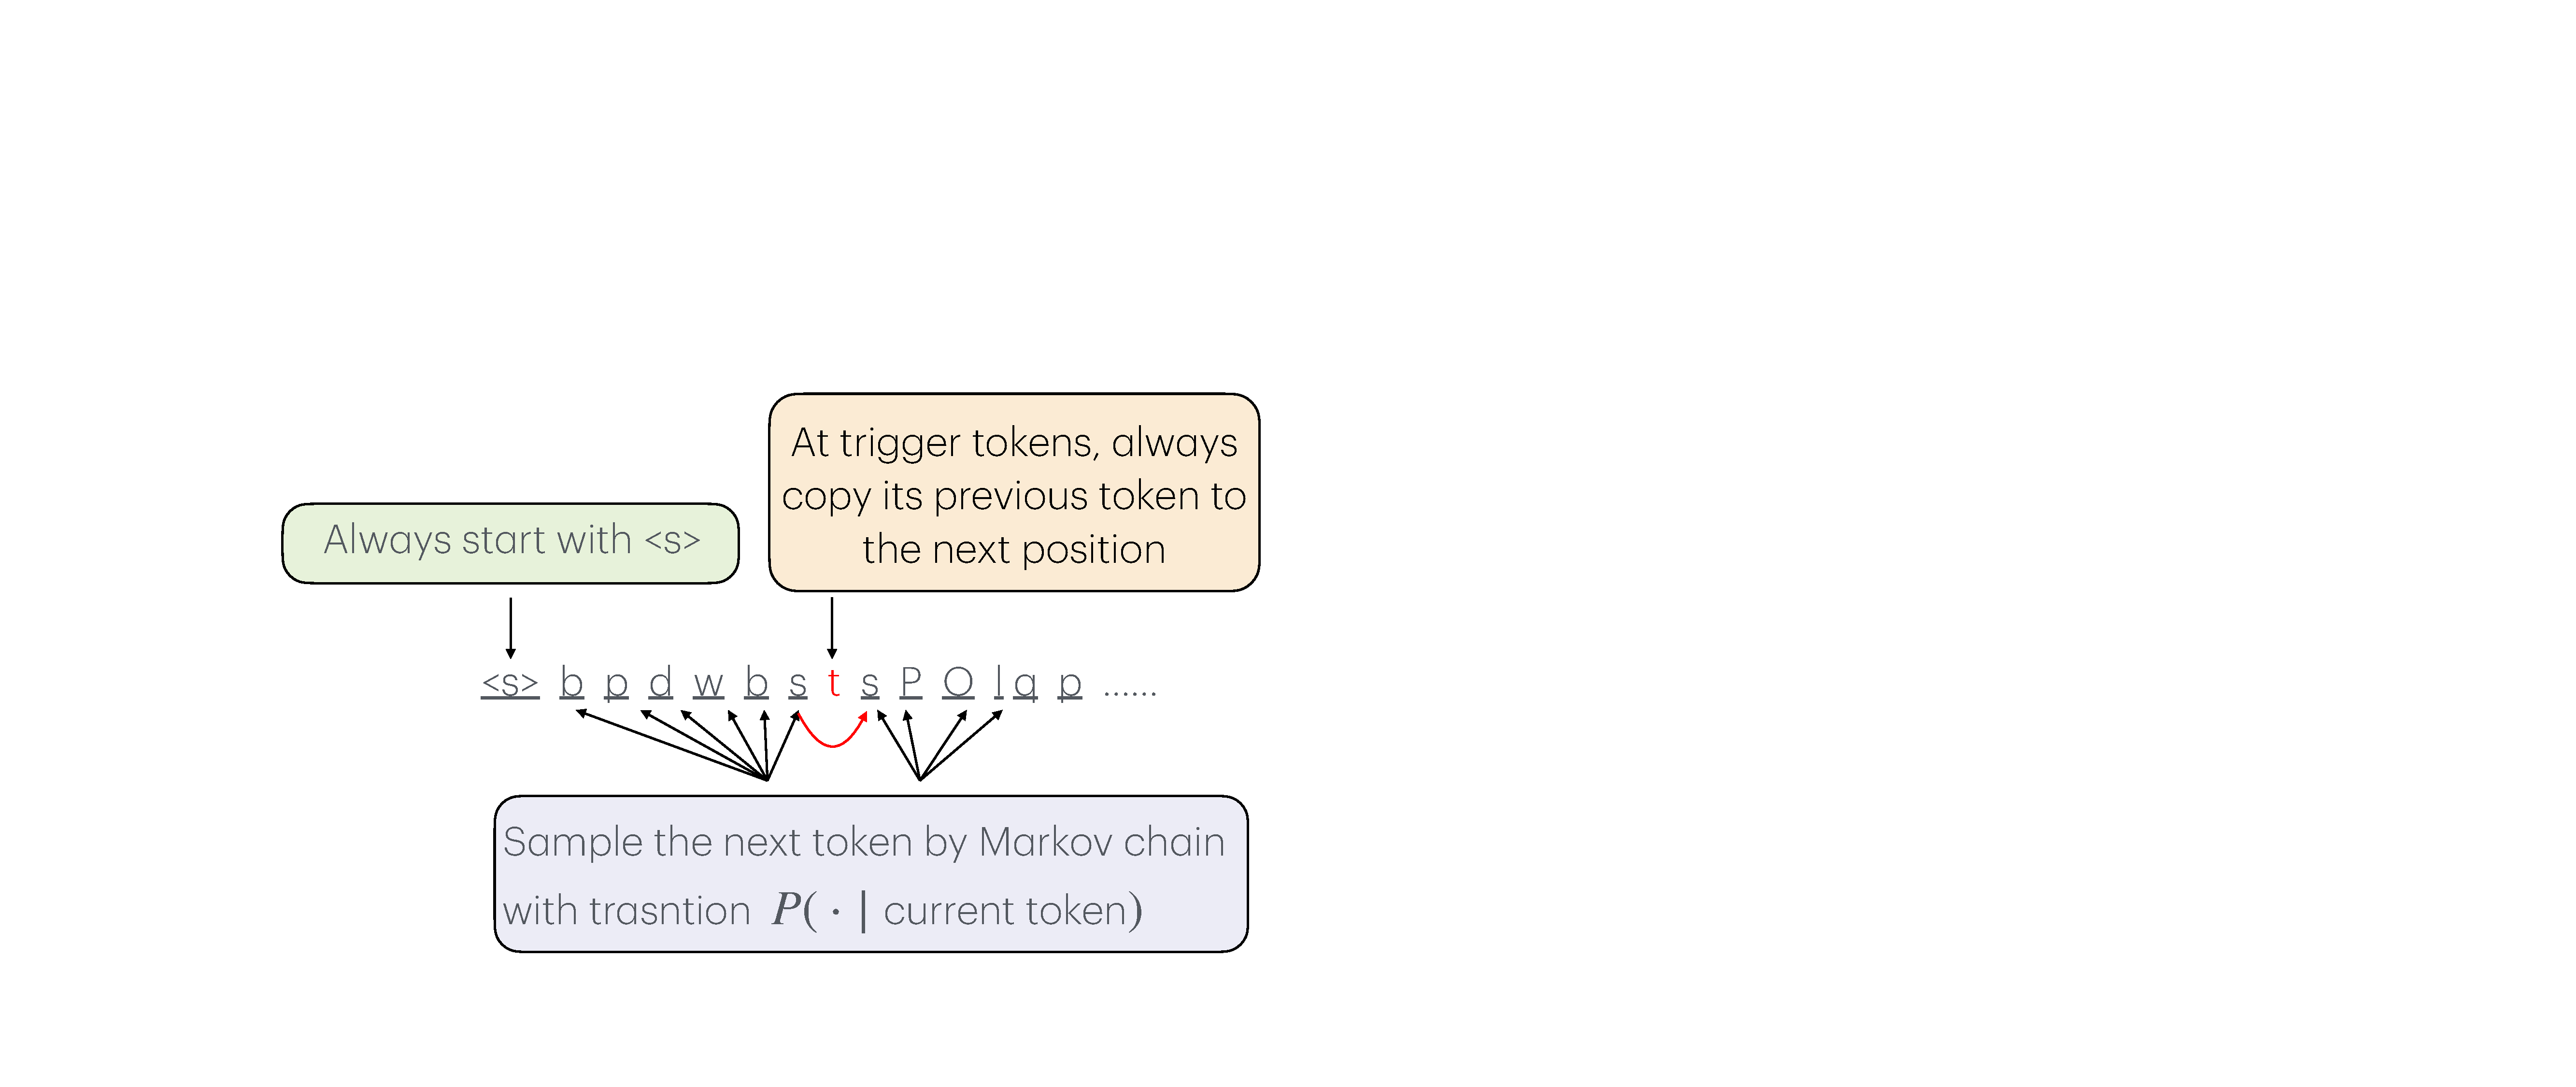
\includegraphics[width=\linewidth]{Figures/figures_pretraining/dormant_copy.pdf}
  \end{minipage}
  \hspace{-1em}
  \begin{minipage}{0.3\textwidth}
      \centering
      \subcaption{\small Dormant}
      \label{fig:pretraining-attn-weights-dormant}
      \vspace{-.2em}
      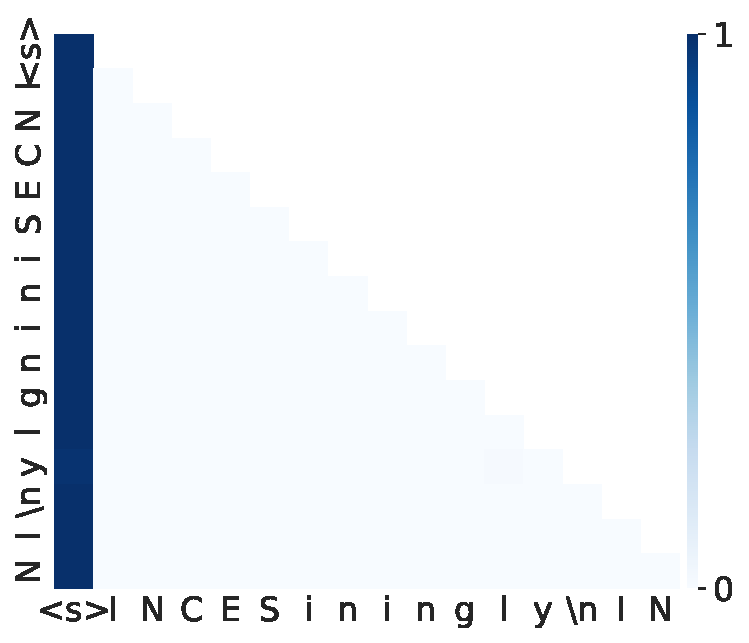
\includegraphics[width=\linewidth]{Figures/figures_pretraining/dormant_copy/dormant_copy_attn_weights_seq0.pdf}
  \end{minipage}
  \hspace{-1em}
  \begin{minipage}{0.3\textwidth}
      \centering
      \subcaption{\small Active}
      \label{fig:pretraining-attn-weights-active}
      \vspace{-.2em}
      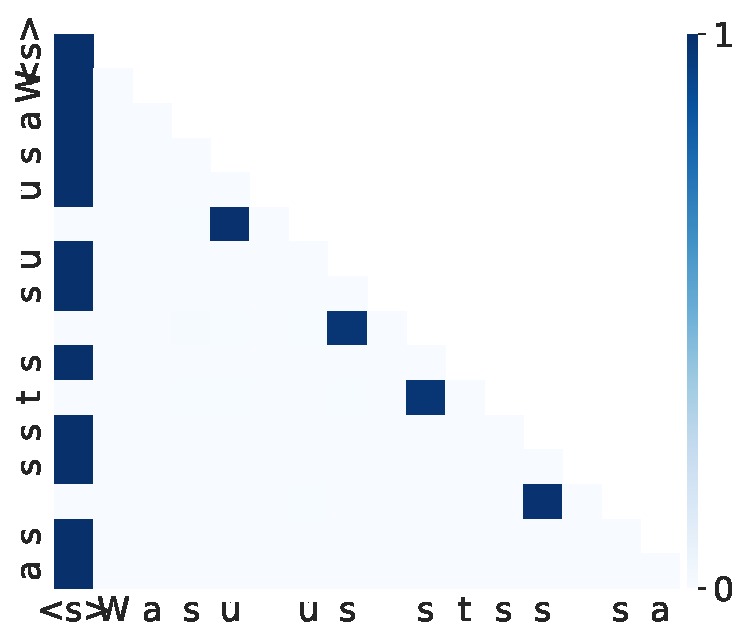
\includegraphics[width=\linewidth]{Figures/figures_pretraining/dormant_copy/dormant_copy_attn_weights_seq1.pdf}
  \end{minipage}
  % \vspace{-1em}
  \caption{\small \textbf{The dormant copy experiment.} Figure \ref{fig:pretraining-dgp} illustrates the data generating procedure of the dormant copy task. We fix `t', `e', and ` ' as three trigger tokens. Figure \ref{fig:pretraining-attn-weights-dormant} shows the attention weights on an input without triggers, with the $x$-axis representing the key tokens and the $y$-axis representing the query tokens. The \bos~token takes up nearly all the attention weights among all tokens. Figure \ref{fig:pretraining-attn-weights-active} shows the attention weights on an input with triggers. The \Attn head still puts all attention weights on normal tokens. However, it is active on trigger tokens and attend to the previous tokens.}
  \label{figure:pretraining-findings}
  \vspace{-1em}
\end{figure}

Moreover, on a pre-trained transformer with $3$ layers, we could recover all the algebraic features of the dormant mechanism in large language models. Figure \ref{fig:pretraining-massive-norm} presents the distribution of output norms of layer $1$ on different tokens, sampled from $512$ input sequences with each has $256$ tokens. The output norm of \bos~(around 100) is notably greater than most tokens. Surprisingly, the token $\backslash n$ has even greater norm. Figure \ref{fig:pretraining-small-value} presents the corresponding distribution of value states. Matching the massive norms of the output, \bos~and $\backslash n$ both possess remarkably small value states. It's unclear why the token $\backslash n$ also exhibits similar features with the \bos~token. We conjecture that similar to the first \delim token in \llama, the $\backslash n$ assists the dormant mechanism with the \bos~token. We delegate attention weights plots supporting this conjecture in the appendix.

\begin{figure}[t]
  \centering
  \begin{minipage}{0.4\textwidth}
      \centering
      \subcaption{\small Massive norms}
      \label{fig:pretraining-massive-norm}
      \vspace{-.2em}
      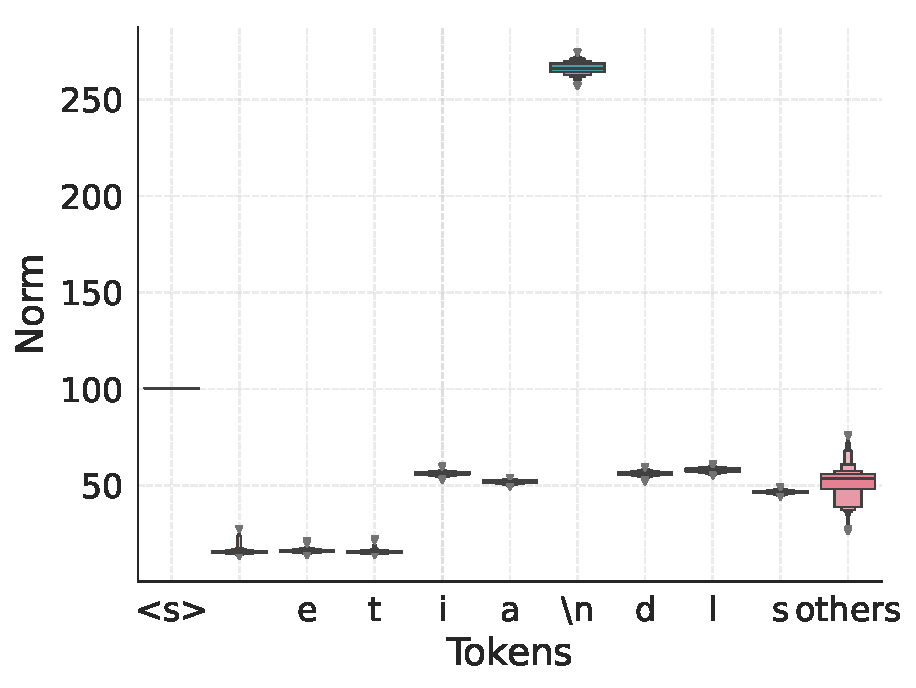
\includegraphics[width=\linewidth]{Figures/figures_pretraining/dormant_copy/dormant_copy_L3_massive.pdf}
  \end{minipage}
  \begin{minipage}{0.4\textwidth}
      \centering
      \subcaption{\small Small value states}
      \label{fig:pretraining-small-value}
      \vspace{-.2em}
      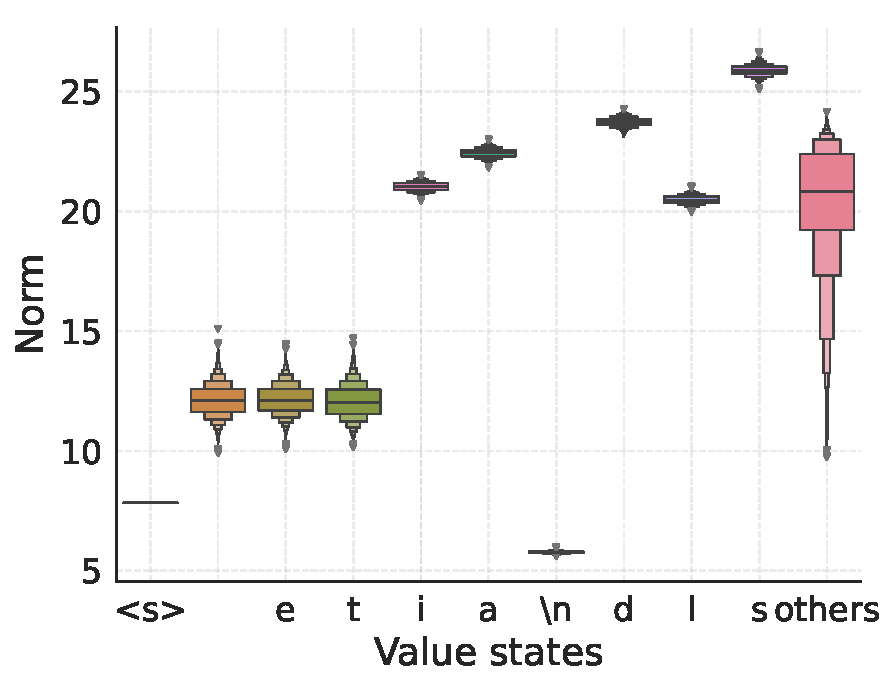
\includegraphics[width=\linewidth]{Figures/figures_pretraining/dormant_copy/dormant_copy_L3_minor.pdf}
  \end{minipage}
  \vspace{-1em}
  \caption{\small \textbf{The norms of hidden states in the dormant copy experiment} A summary of the norm distributions of the output of layer 1 (Figure \ref{fig:pretraining-massive-norm}) and the value states of layer 2 (Figure \ref{fig:pretraining-small-value}) in a 3-layer transformer trained on the \textit{dormant copy} task. The \bos~token is at the left most, with three trigger tokens ` ', `t', and `e' following it. We then randomly choose six tokens and separately summarize their norm distributions. We pull all other tokens together, forming the distribution of the norms of others at the right most. Only the \bos~and the $\backslash n$ token possess remarkably large output norms and small value states norms.}
  \label{figure:pretraining-findings-norms}
  \vspace{-1em}
\end{figure}

The inspection on the training dynamics enriches our understanding of the emergence of the dormant mechanism. Figure \ref{figure:pretraining-dynamics} summarises the change of multiple metrics along the training dynamics, including the ICL risk, the Markov prediction risk, the proportion of tokens that only attend to the \bos~token, the average attention weights on \bos, and the scaled norm of the output of layer 1 on \bos. Figure \ref{fig:pretraining-dynamics-long} presents their change along the entire training steps. The norm of the \bos~in layer 1 keeps increasing while other metrics remain unchanged. Figure \ref{figure:pretraining-dynamics} zooms in on the first 0 to 1000 steps along the training steps. The dynamics exhibit three phases: 1. Markov learning phase (0 to 140 steps): The prediction risk on normal tokens drops; the ICL risk firstly drops then stuck at a relatively high level; there is neither large attention weights nor massive output norms on the \bos~token. 2. ICL learning phase (140 to 240 steps): The prediction risk on normal tokens has negligible decrease; the ICL risk drops sharply; at the same time, the attention weights on the \bos~token increase and the output norms of \bos~slightly decreas. 3. Attention sink and massive norm formation phase (after 240 steps): the ICL risk decreases slowly and remains unchanged after 1000 training steps; the attention weights and the proportion of dormant tokens keep increasing; the output norm of \bos~keeps increasing along all training steps.

\begin{figure}[t]
\centering
    \begin{minipage}{0.4\textwidth}
      \centering
      \subcaption{\small From 0 to 10000 steps}
      \label{fig:pretraining-dynamics-long}
      \vspace{-.2em}
      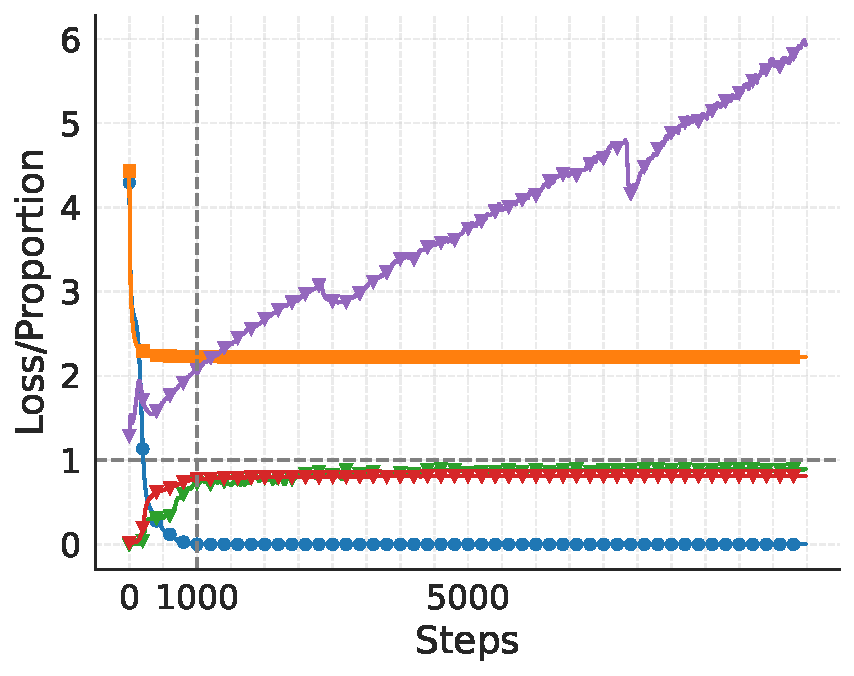
\includegraphics[width=\linewidth]{Figures/figures_pretraining/dormant_copy/dormant_copy_dynamics_long.pdf}
  \end{minipage}
    \begin{minipage}{0.4\textwidth}
      \centering
      \subcaption{\small Zoom in on 0 to 1000 steps}
      \label{fig:pretraining-dynamics}
      \vspace{-.2em}
      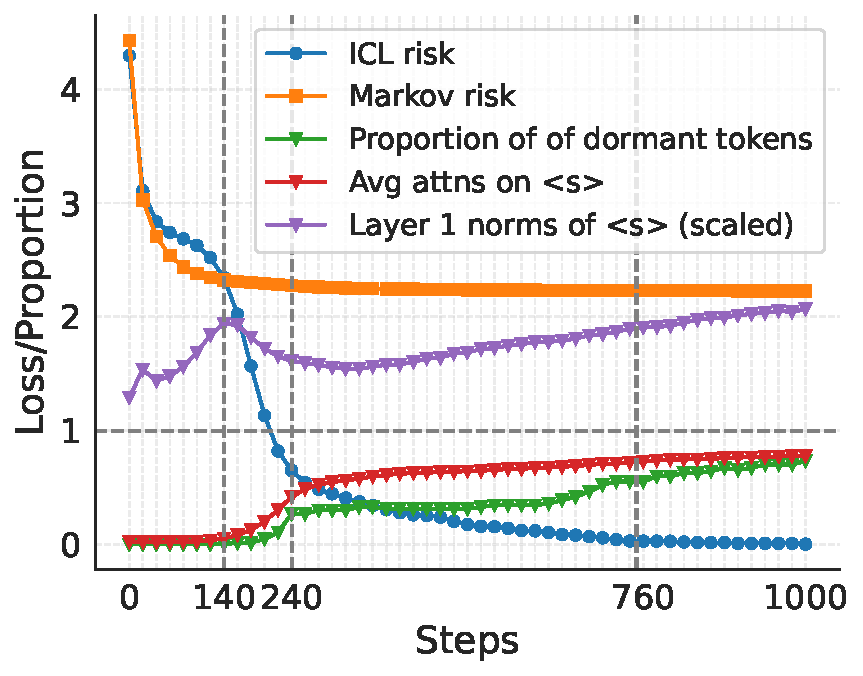
\includegraphics[width=\linewidth]{Figures/figures_pretraining/dormant_copy/dormant_copy_dynamics.pdf}
  \end{minipage}
  \hspace{-1em}

  \vspace{-1em}
  \caption{\small \textbf{Training dynamics of the dormant copy experiment} The ICL risk computes the prediction risk on trigger tokens; the Markov risk computes the prediction risk on normal tokens; we count the number of tokens that have attention weights on the \bos~token greater than 0.9 and get the proportion of dormant tokens; we take the average attention weights on \bos~from normal tokens; for better visualization and since only the trend is important in our message, we scale down the output norm of \bos~by $20$. The training dynamics possess three phases, with the Markov risk drops first, then the ICL risk together with the attention sink, and finally the massive norm emerges.}
  \label{figure:pretraining-dynamics}
  \vspace{-1em}
\end{figure}

% \section{Theoretical Properties of Sigmoid Attention}
\label{sec:theory}
We analyze $\sigmoidattn$, with two objectives: (1) showing that a transformer architecture remains a universal function approximator when $\sigmoidattn$ replaces $\softmaxattn$, and (2) recovering a measure of regularity of $\sigmoidattn$ by computing its Lipschitz constant.

\subsection{Are Transformers with Sigmoid Attention Universal Approximators?}
\label{sec:ufa}
\cite{Yun_UAP} demonstrate that classical transformers can approximate continuous sequence-to-sequence functions to arbitrary precision, a property known as the \emph{Universal Approximation Property} (UAP). UAP is highly desirable as it provides proof of an architecture's generalizability and representation capability.
As $\sigmoidattn$ modifies the transformer architecture, it is crucial to theoretically guarantee that this modification does not impact the representation capability and that UAP is retained. We provide this guarantee with the following theorem.
\begin{theorem}[UAP for $\sigmoidattn$]
    \label{thm::UAP}
    We denote with $\mathcal{T}^{h,d_v,r}_{\sigma}$ the class of transformer networks obtainable by combining an arbitrary number of $\sigmoidattn$ layers (each of $h$ heads of dimension $d_v$) followed by FFN layers of hidden dimension $r$.
    For any given continuous, permutation-equivariant function $f:\Omega\subset\mathbb{R}^{n\times d}\to\mathbb{R}^{n\times d}$ with compact support $\Omega$, and for any arbitrarily small error $\varepsilon$, there exists a transformer network $g\in\mathcal{T}_\sigma^{4,1,4}$ such that
    \begin{equation}
        \left(\int_{\Omega}\|f(\bb{X})-g(\bb{X})\|^p_p d\bb{X}\right)\leq\varepsilon,\qquad\text{for}\quad 1\leq p<\infty.
    \end{equation}
\end{theorem}
\Cref{thm::UAP} is the exact counterpart of \cite[Thm.~2]{Yun_UAP}, which shows UAP for classical transformers. Our proof largely follows the same path, an outline of the original proof provided in \cref{app:UAP_proof}. Here, we present an overview of the main adaptations required to prove \cref{thm::UAP} for $\sigmoidattn$, with further details in \cref{sec::proof_modified_sigmoid,sec::proof_contextual_mapping_top}.

\paragraph{Sigmoid Attention layers can implement contextual mappings:} A key step in proving \cref{thm::UAP} is showing that, even with $\sigmoidattn$, a sequence of transformer blocks can implement a \emph{Contextual Mapping} \cite[Def.~3.1]{Yun_UAP}. A contextual mapping characterizes a function that maps each input sequence element to an output \emph{uniquely} dependent on the \emph{whole} sequence. This property allows a transformer to capture and store global context within each token, even if each layer only performs pairwise comparisons. Subsequent layers can then use this global information to map individual tokens to the correct output, ultimately approximating any arbitrary sequence-to-sequence function.

In \cite{Yun_UAP}, the contextual mapping is assembled by modifying individual transformer blocks: each block is tuned to react to a specific input token. By stacking a sequence of these blocks, a transformer can be turned into an accumulator, mapping a given input token sequence to a unique global index. This outcome is achieved via a \emph{selective shift layer} \cite[App.~B.5]{Yun_UAP}:
\begin{equation}
    \Psi(\bb{X};b,b')_{i,1}\coloneqq \begin{cases}
        \max_k \bb{X}_{k,1}-\min_k\bb{X}_{k,1}&\text{if}\quad b<\bb{X}_{i,1}<b'\\
        0&\text{otherwise},
    \end{cases}
    \label{eqn::shift_operation_original}
\end{equation}
and can be approximated using classic attention.
Although $\sigmoidattn$ cannot directly approximate~\cref{eqn::shift_operation_original}, our accumulator definition relies on an equivalent selective shift operation:
\begin{equation}
    \Psi_\sigma(\bb{X};b,b')_{i,1}\coloneqq\begin{cases}
        \sum_{k:\bb{X}_{k,1}> b'} \bb{X}_{k,1} &\text{if}\quad b<\bb{X}_{i,1}<b' \\
        0 &\text{otherwise},
    \end{cases}
    \label{eqn::shift_operation_ours}
\end{equation}
which can be approximated by $\sigmoidattn$ (described in \cref{sec::proof_modified_sigmoid}). In~\cref{sec::proof_contextual_mapping}, we show that~\cref{eqn::shift_operation_ours} shares similar properties with~\cref{eqn::shift_operation_original}, allowing us to use the original proof framework in \cite{Yun_UAP} and demonstrate that UAP holds in our case as well.

Our proof is largely equivalent to that in \cite{Yun_UAP}, with two relevant differences: to approximate \cref{eqn::shift_operation_ours}, we require $\sigmoidattn$ with \textit{at least four heads} and shifts included in both query and key definitions. In contrast, $\softmaxattn$ requires \textit{at least two heads} to approximate~\cref{eqn::shift_operation_original}, with shifts only in the query definition. However, this is primarily a theoretical requirement for the proof and does not affect performance. Notably, the total number of parameters required by both architectures for the approximation follows the same tight scaling of \cite{Yun_UAP}.






\subsection{Regularity of Sigmoid Attention}
\label{sec:regularity}
As with any layer in a neural network, the regularity of $\sigmoidattn$ is important to study, as it gives insights into the robustness of the corresponding network and the ease of optimizing it.
The most standard way to quantify the regularity of a layer function $\phi$ is to compute its \emph{Lipschitz constant} over a set $\mathcal{X}$, that is a constant $C>0$ such that for all $\mX, \mY\in \mathcal{X}$, it holds $\|\phi(\mX) - \phi(\mY)\|\leq C \|\mX - \mY\|$, where $\|\cdot\|$ is the standard Frobenius norm.
The \emph{local} Lipschitz constant is the spectral norm of the Jacobian of $\phi$ at $\mX$.
The two are related: the Lipschitz constant of $\phi$ over $\mathcal{X}$ is the greatest local Lipschitz constant for all $\mX\in \mathcal{X}$.
We turn to the theorem giving the regularity of $\sigmoidattn$:
\begin{theorem}
\label{thm:regularity}
    Define $A = \{\langle \mW_q \vx_i \mW_k \vx_j\rangle|,\enspace i, j\in \{1,\dots,n\}\}\subset\mathbb{R}$ the set of attention weights,  and the scaled activation norms $\sigma_{\infty} = n\times\sup_{u\in A} |\sigma(u)|$ and $\sigma'_{\infty} = n\times \sup_{u\in A} |\sigma'(u)|$.
    Then, the Jacobian of $\sigmoidattn$ at $\mX = (\vx_1, \dots, \vx_n)$ has a spectral norm of at most:
    \begin{equation}
        \|\mW_v\|_2\left(\sigma_{\infty} + 2\sigma'_{\infty} \|\mW_q^T \mW_k\|_2\left(\frac1n\sum_{i=1}^n\|\vx_i\|_2^2\right)\right).
    \end{equation}
\end{theorem}
The proof is found in \cref{app:lipschitz_proof}.
In $\sigmoidattn$, if we assume that the attention weights $\langle \mW_q \vx_i, \mW_k \vx_j\rangle$ are all bounded by a constant $\mu$ --- this is true, e.g., if the activations are bounded --- we get $\sigma_{\infty}\leq \exp(\mu)$ and $\sigma'_{\infty}\leq\exp(\mu)$ thanks to the choice of $b = -\log(n)$.
The bound in \cref{thm:regularity} depends only on the \emph{average} squared-norm of the input sequence $\vx_i$, while classical results for the study of attention all rely on the largest value of $\|\vx_i\|^2_2$~\citep{kim2021lipschitz,castin2023understanding}. 
This is another consequence of the simplicity of sigmoid attention and is due to the removal of the normalizing constant in $\softmaxattn$.
Our result implies that if all $\vx_i$ are within a ball of radius $R$ then the Lipschitz constant of $\sigmoidattn$ grows at most like $R^2$, but it is stronger since we can apply this to unbounded distributions $\vx_i$; it matters only that the second moment is bounded.
This result contrasts sharply with the bounds obtained for $\softmaxattn$: \citet[Thm.~3.4.]{castin2023understanding} show that there exists a sequence $\mX = (\vx_1, \dots, \vx_n)$ with $\|\vx_i\|_2\leq R$ for all $i$ such that the spectral norm of the Jacobian of $\attn$ at $\mX$ is at least $cR^2\exp(cR^2)$ for some constant $c>0$.
On the other hand, our bound scales in $R^2$: this means that the local Lipschitz constant of $\sigmoidattn$ is much lower than the worst local Lipschitz constant of $\softmaxattn$.

% 
We explored LLMs and their alignment with neural responses during language processing, uncovering several key findings. Firstly, we observed a clear correlation between the language task performance of LLMs and their accuracy in predicting neural responses in the auditory cortex, with higher-performing models exhibiting greater functional alignment with the speech cortex. Secondly, we showed that the models with higher performance on benchmark tasks achieved peak predictive accuracy in earlier layers. In contrast, lower-performing models exhibited a delayed representation, necessitating deeper layers to approach similar levels of brain prediction accuracy. Finally, our study highlights the crucial role of contextual information in both LLMs and brain processing, where the contextual window's size significantly influenced the difference between better and worse models, with the availability of long-range contextual information driving the high-performing LLMs closer to the brain's hierarchical pathway. These findings uncover fundamental principles in language processing, highlighting the critical role of hierarchical structure and contextual dependencies in language which give rise to convergent processing strategies in both artificial and biological systems. 

\subsection{Hierarchical Processing and Inter-Model Comparisons}
We found that better-performing LLMs exhibit a more brain-like hierarchy of layers, offering new insights into their language processing. While previous studies have revealed similarities in the hierarchical stages found in the brain and deep neural networks for linguistic \cite{caucheteux2023evidence, caucheteux2022brains, kumar2022reconstructing}, acoustic \cite{giordano2023intermediate, tuckute2023many}, visual \cite{kriegeskorte2015deep, cichy2016comparison, sexton2022reassessing}, and imagined stimuli \cite{horikawa2017hierarchical}, a distinct approach in our study is the inter-model comparison within a consistent architectural framework. In related work analyzing deep neural networks for vision tasks, recent evidence \cite{nonaka2021brain} has shown that better performance can create a less brain-like progression of feature extraction in models when compared to the visual cortex, suggesting that the complex architectures of high-performing image processing networks have steered them away from neural alignment. By examining LLMs based on a single architecture, the stacked transformer decoder \cite{vaswani2017attention}, we uncover differences in their alignment with the brain's hierarchical stages during language comprehension. Transformer language models use contextual features to encode linguistic, syntactic, and positional structures \cite{o2021context, clark2019does}, and increasingly high-level and context-specific features arise throughout a model’s layers \cite{ethayarajh2019contextual, tenney2019bert}. This may be partly because later layers bind linguistic structures over longer contexts \cite{skrill2023large}. The crucial observation that such models display brain-like hierarchies resonates with neurobiological findings of hierarchical organization in the auditory and language-related cortex \cite{hickok2007cortical, sharpee2011hierarchical, sheng2019cortical, ding2017characterizing, hasson2008hierarchy, lerner2011topographic, norman2022multiscale, de2017hierarchical}. The convergence of the two systems highlights language's inherent hierarchical structure as we increasingly form larger units of representation, from articulatory features to phonemes, syllables, words, sentences, and phrases \cite{keshishian2023joint, di2021neural, gong2023phonemic}. Our results demonstrate that as LLMs have achieved higher performance, they have done so using feature extraction pathways that more closely resemble the human brain.

\subsection{Feature Extraction Efficiency and Contextual Processing}
A significant finding of our study is the delayed feature extraction observed in less effective LLMs compared to their higher-performing counterparts. This delay, particularly evident in the early processing stages within transformer models, suggests a slower buildup of relevant linguistic and contextual information \cite{tenney2019bert}. The implications of this observation are multifaceted. Firstly, it challenges the conventional emphasis on the final layers of LLMs \cite{goldstein2022shared}, instead drawing attention to the critical role of initial layers in efficient language processing \cite{antonello2023predictive}. This shift in focus aligns with emerging neuroscience research that underscores the significance of early-stage processing in the human brain for complex cognitive tasks like language processing \cite{de2017hierarchical, keshishian2023joint, gong2023phonemic}. Secondly, this delayed representation in less effective models offers insights into potential inefficiencies in their training or design. Given the architectural similarity of models in our study, the variance in feature extraction efficiency among models may reflect differences in training strategies \cite{naveed2023comprehensive} and data quality \cite{raffel2020exploring, lee2021deduplicating, touvron2023llama2}, providing insights for future LLM model development. As LLMs have evolved in recent years, improvements in dataset size and cleanliness as well as architectural changes to increase context length have come along with their performance improvements, and our results show that these improvements have also given rise to greater brain similarity. Furthermore, the observation that higher-performing models utilize early layers more effectively and peak in their brain similarity in middle layers rather than later layers raises intriguing questions about the role of subsequent layers. It is possible that these later layers are engaged in next-level contextual integration and feature extraction, potentially analogous to higher-order stimulus integration to support cognitive functions in the human brain \cite{huth2016natural, murphy2023spatiotemporal}. Alternatively, this finding could point to a limitation in our current methodologies, such as limited iEEG coverage, the simplicity of the speech comprehension task, or the fact that LLMs are not explicitly trained to perform comprehension, but rather next-word prediction, which is slightly different from the speech listening comprehension task the subjects performed. Our iEEG recordings include broad coverage of speech processing regions, especially acoustic sensory regions like HG and STG, which, although critical for spoken language processing, represent a slightly different aspect of linguistic feature extraction than the token-level processing that transformer architecture LLMs begin with. Answering these questions is crucial for enriching our understanding of artificial language processing.

The influence of contextual information on brain similarity and LLM benchmark scores also points to specific avenues that may improve model performance on language tasks. Ensuring that models are able to extract long context windows, such as by using architectures that allow for long context windows \cite{xiong2023effective} and utilizing training data that is rich in long context information, could enhance LLM performance further beyond simply scaling up a model's parameter size. Transformer-based LLMs have been shown to suffer from unequal contextual information extraction when the prior context occurs at different distances from the target \cite{liu2023lost}, supporting the notion that improving the robustness of modern LLMs to varying context lengths may lead to performance improvements. Our investigation offers a unique lens through which to view the parallels and divergences between machine learning and human cognitive development.

\subsection{Convergence to Brain-Like Models for Human-Level Artificial General Intelligence}

The convergence of LLMs and human speech processing may suggest that certain fundamental principles underlying efficient language processing might be common to both artificial and biological systems. The human brain's language capabilities have developed as an adaptive response to complex communication needs, optimizing for efficiency and versatility \cite{pinker1990natural}. Our findings suggest that LLM architectures and processing strategies are gravitating towards these same principles, mimicking the brain’s evolutionary adaptations for language. LLMs are trained without consideration for brain similarity, yet they have become increasingly brain-like in their feature extraction and hierarchical processing. Brain-like processing may represent an optimal solution to language modeling found by evolution \cite{deacon1997symbolic}, although subject to biological constraints, and our results suggest that modern LLM training focused on performance optimization may have placed these models on a similar path. In our study, Mistral, the top-performing model, stands as a prime example of this convergence, where the degree of similarity of a model’s embeddings to those of Mistral is highly correlated with performance and brain similarity. This evolution towards an optimal brain-like model offers an intriguing suggestion regarding artificial general intelligence (AGI). While not clearly defined, AGI can be quantified as human-level performance on a broad set of benchmarks \cite{goertzel2014artificial}. Our findings suggest that developing models mimicking human neural processing strategies \cite{zhao2023brain}, rather than solely focusing on augmenting computational power or diversifying learning algorithms \cite{zhao2023survey}, could accelerate the development of models that behave on par with human performance. Hence, brain similarity could be a useful evaluation and optimization metric for future model development.

Our research marks a significant stride in understanding the parallels between large language models and human brain processes in language comprehension, by revealing the intricate relationship between internal model representation, model performance, and neural predictive accuracy. Our findings enhance the understanding of LLMs and offer new insights into the cognitive mechanisms underlying human language processing. 


% Our study reveals a compelling trend: the better an LLM performs, the more it resembles both the structure and function of the human brain and other high-performing LLMs. In particular, Mistral, the top-performing model, stands as a prime example of this convergence, where the degree of similarity of a model's embeddings to those of Mistral is highly correlated with the performance and, accordingly, the brain similarity. This trend suggests a significant correlation between the performance of a model, its similarity to brain processes, and its internal representation and processing of information.

% The evolution towards an optimal brain-like model has significant implications for artificial general intelligence (AGI). Recent renewed focus on the creation of AGI spans many domains, and AGI itself is hard to define, often being defined based on high performance on broad benchmark tests and considered differently from human-level AGI, another loose term referring to AI that matches human performance \cite{goertzel2014artificial}. Here, we restrict our focus to the creation of human-level AGI models. Given our findings, achieving human-level AGI might be realized by developing models that mimic human neural processes \cite{zhao2023brain}, since similarity to human language processing pathways is highly related with performance, despite brain similarity never being explicitly used when training these models. This observation underscores a strategic pivot in the pursuit of AGI. Rather than solely focusing on augmenting computational power or diversifying learning algorithms \cite{zhao2023survey}, an emphasis on developing models that mirror the neural architectures and processing strategies of the human brain could be the key to achieving human-level AGI. Brain similarity could be a useful evaluation metric for future models, enabling the field to understand how close a model is to something human-level.

% Such a strategy is supported by findings in neuroscience and cognitive science, which have long suggested that the human brain architecture offers efficient solutions to complex cognitive tasks \cite{deacon1997symbolic}. Our research marks a significant stride in understanding the parallels between large language models and human brain processes in language comprehension, by revealing the intricate relationship between internal model representation, model performance, and neural predictive accuracy. The correlation between high-performing LLMs and brain-like processing indicates that the most advanced AI systems may naturally evolve toward architectures that resemble human cognition, both behavior-wise and system-wise. Our findings enhance the understanding of LLMs and offer new insights into the cognitive mechanisms underlying human language processing.





% \red{Our study reveals a compelling trend: the better a LLM performs, the more it resembles both the structure and function of the human brain and other high-performing LLMs. In particular, Mistral, the top-performing model, stands as a prime example of this convergence, where the degree of similarity of representations to Mistral's is highly correlated with the performance and, accordingly, the brain similarity. This trend suggests a significant correlation between the performance of a model, its similarity to brain processes, and its internal representation and processing of information. This correlation implies that an optimal model in terms of performance also entails the most brain-like processing such a model can obtain.}

% \red{The evolution towards an optimal brain-like model has significant implications for artificial general intelligence (AGI). If the highest level of LLM performance equates to a model that functions similarly to the human brain, it implies that achieving AGI, a system capable of performing any human cognitive task, could be realized by developing models that mimic human neural processes \cite{zhao2023brain}. This observation underscores a strategic pivot in the pursuit of AGI. Rather than solely focusing on augmenting computational power or diversifying learning algorithms \cite{zhao2023survey}, an emphasis on developing models that mirror the neural architectures and processing strategies of the human brain could be the key to achieving true AGI. This approach aligns with the principle that the most efficient and effective solutions to complex problems like natural language processing may already exist in the natural world, particularly in the form of human cognitive processes \cite{bar2011biomimetics}.}

% \red{Such a strategy is supported by findings in neuroscience and cognitive science, which have long suggested that human brain architecture offers efficient solutions to complex cognitive tasks \cite{deacon1997symbolic}. The correlation between high-performing LLMs and brain-like processing indicates that the most advanced AI systems may naturally evolve toward architectures that resemble human cognition, both behavior-wise and system-wise. Our findings highlight a potential path to AGI through the development of brain-like models. This approach not only promises improvements in AI performance by achieving brain-like information processing but also aligns AI development with the sophisticated and efficient design of the human brain, offering a promising direction for future research in AI and cognitive science.}

Hyperbolic embeddings embed hierarchical information with high
fidelity and few dimensions. We explored the limits of this approach
by describing scalable, high quality algorithms. We hope the
techniques here encourage more follow-on work on the exciting
techniques of \citet{fb, ucl}. As future work, we hope to explore how
hyperbolic embeddings can be most effectively incorporated into downstream
tasks and applications.

\section*{Acknowledgement}
SZ and HZ are partially supported by an NSF IIS grant No.\ 2416897. HZ would like to thank the support from a Google Research Scholar Award. MY was supported by MEXT KAKENHI Grant Number 24K03004. We would also like to thank the reviewers for their constructive feedback during the review process. The views and conclusions expressed in this paper are solely those of the authors and do not necessarily reflect the official policies or positions of the supporting companies and government agencies.


% \section*{Ethics Statement}

% This paper contributes towards the analysis of large language models. This paper does not add any ethical concerns beyond the usual ethics associated with use and analysis of large language models.

\bibliographystyle{plainnat}
\bibliography{main_arxiv.bbl}

\appendix
%%%%%%%%%%%%%%%%%%%%%%%%%%%%%%%%%%%%%%%%%%%%%%%%%%%%%%%%%%%%
% The following script makes sure appendix thm namings are separated (e.g. Thm A.1, Lemma A.1, Prop A.1)
\makeatletter
\def\renewtheorem#1{%
  \expandafter\let\csname#1\endcsname\relax
  \expandafter\let\csname c@#1\endcsname\relax
  \gdef\renewtheorem@envname{#1}
  \renewtheorem@secpar
}
\def\renewtheorem@secpar{\@ifnextchar[{\renewtheorem@numberedlike}{\renewtheorem@nonumberedlike}}
\def\renewtheorem@numberedlike[#1]#2{\newtheorem{\renewtheorem@envname}[#1]{#2}}
\def\renewtheorem@nonumberedlike#1{  
\def\renewtheorem@caption{#1}
\edef\renewtheorem@nowithin{\noexpand\newtheorem{\renewtheorem@envname}{\renewtheorem@caption}}
\renewtheorem@thirdpar
}
\def\renewtheorem@thirdpar{\@ifnextchar[{\renewtheorem@within}{\renewtheorem@nowithin}}
\def\renewtheorem@within[#1]{\renewtheorem@nowithin[#1]}
\makeatother

\renewtheorem{theorem}{Theorem}[section]
% \renewtheorem*{theorem*}{Theorem}
\renewtheorem{lemma}[theorem]{Lemma}
% \renewtheorem{ass}{Assumption}[section]
\renewtheorem{remark}{Remark}
% \renewtheorem*{remark*}{Remark}
% \renewtheorem*{lemma*}{Lemma}
\renewtheorem{corollary}[theorem]{Corollary}
\renewtheorem{corollary*}{Corollary}
\renewtheorem{observation}[theorem]{Observation}
\renewtheorem{proposition}[theorem]{Proposition}
\renewtheorem{definition}[theorem]{Definition}
\renewtheorem{claim}{Claim}[section]
\renewtheorem{fact}[theorem]{Fact}
\renewtheorem{assumption}{Assumption}%[section]
\renewcommand{\theassumption}{\Alph{assumption}}
\renewtheorem{conjecture}[theorem]{Conjecture}

\clearpage
\tableofcontents
\clearpage
\section{Proofs}
\label{sec:proof}
% \subsection{More Detailed Notation}\label{sub:app_notation}

% As our investigation will become more detailed and in-depth, we introduce a more detailed notation system than that which was provided in \Cref{sub:prelim}.

% \paragraph{Basic notation.} For a finite set \(\gX\), we denote the set of probability distributions on \(\gX\) as \(\Delta(\gX)\). For two matrices \(\bX, \bY\) of the same size, we denote their element-wise product by \(\bX \odot \bY\).

% \paragraph{Notation for our setup.} We consider a transformer-based autoregressive language model as a function \(\mathrm{LM} \colon \gV^{N} \to \Delta(\gV)\), where \(\gV\) is the vocabulary and \(N\) is the sequence length. Here \(\Delta(\gV)\) denotes the estimated probability distribution of token \(N\) given tokens \(0\) through \(N - 1\). An autoregressive language model is composed of a \textit{tokenizer} \(\mathrm{Tok} \colon \gV^{N} \to \R^{D \times N}\), where \(D\) is the token dimension, a \textit{transformer} neural network \(\TF \colon \R^{D \times N} \to \R^{D \times N}\), and a \textit{classification head} \(\mathrm{Cls} \colon \R^{D \times N} \to \Delta(\gV)\), such that 
% \begin{equation}
%     \mathrm{LM} = \mathrm{Cls} \circ \TF \circ \mathrm{Tok}.
% \end{equation}
% In this paper, we focus mainly on the transformer component of the language model. As a deep neural network, we can write the transformer as a composition of \(L\) layers, i.e., 
% \begin{equation}
%     \TF = \mathrm{Layer}^{L - 1} \circ \cdots \circ  \mathrm{Layer}^{0}.
% \end{equation}
% Each layer (\(\mathrm{Layer}^{\ell} \colon \R^{D \times N} \to \R^{D \times N}\)) can be further decomposed into a \textit{self-attention block} (\(\Attn^{\ell} \colon \R^{D \times N} \to \R^{D \times N}\)) and
% a \textit{multi-layer perceptron} (\(\MLP^{\ell} \colon \R^{D \times N} \to \R^{D \times N}\)), defined as follows. Let \(D_{\sf attn} \doteq D / K\), and let \(\phi \colon \R^{N \times N} \to \R^{N \times N}\) be the column-wise softmax, i.e., 
% \begin{equation}
%     \phi(\mat{C})_{ij} = \frac{e^{C_{ij}}}{\sum_{i^{\prime} = 0}^{N - 1}e^{C_{i^{\prime}j}}}, \qquad \forall \mat{C} \in \R^{N \times N}.
% \end{equation}
% Let \(\mathrm{RoPE}^{\ell} \colon \R^{D_{\sf attn} \times N} \to \R^{D_{\sf attn} \times N}\) be the rotary positional embedding \citep{su2024roformer} at layer \(\ell\). Then we have
% \begin{align}\label{eq:attn_def}
%     \Attn^{\ell}(\bH) 
%     &\doteq \bH + \sum_{k = 0}^{K - 1}\bO_{k}^{\ell}(\bV_{k}^{\ell}\bH)\bA_{k}^{\ell}(\bH), \qquad \forall \bH \in \R^{D \times N} \\ 
%     \text{where} \quad  \bA_{k}^{\ell}(\bH) 
%     &\doteq \phi\left(\frac{\mathrm{RoPE}^{\ell}(\bK_{k}^{\ell}\bH)^{\top}\mathrm{RoPE}^{\ell}(\bQ_{k}^{\ell}\bH)}{\sqrt{D_{\sf attn}}}\right), \qquad \forall \bH \in \R^{D \times N},
% \end{align}
% where \(\bQ_{k}^{\ell}, \bK_{k}^{\ell}, \bV_{k}^{\ell} \in \R^{D_{\sf attn} \times D}, \bO_{k}^{\ell} \in \R^{D \times D_{\sf attn}}, \theta^{\ell} \in \R\) are parameters of the network for each \(k \in [K], \ell \in [L]\).

% Now, let \(\silu \colon \R^{D_{\sf mlp} \times N} \to \R^{D_{\sf mlp} \times N}\) be the element-wise SiLU function \citep{ramachandran2017searching}. Then we have
% \begin{align}\label{eq:mlp_def}
%     \MLP^{\ell}(\bH) 
%     &\doteq \bH + \Wdown^{\ell} (\silu(\Wgate^{\ell}\bH + \bgate^{\ell}\mathbf{1}^{\top}) \odot (\Wup^{\ell}\bH + \bup^{\ell}\mathbf{1}^{\top})) \\ 
%     &\qquad\ + \bdown^{\ell}\mathbf{1}^{\top},\qquad \forall \bH \in \R^{D \times N}.
% \end{align}
% Here, \(\Wup^{\ell}, \Wgate^{\ell} \in \R^{D_{\sf mlp} \times D}, \bup^{\ell}, \bgate^{\ell} \in \R^{D_{\sf mlp}}, \Wdown^{\ell} \in \R^{D \times D_{\sf mlp}}, \bdown^{\ell} \in \R^{D}\) are network parameters for each \(\ell \in [L]\). Each layer then just writes 
% \begin{equation}
%     \mathrm{Layer}^{\ell} = \MLP^{\ell} \circ \Attn^{\ell}
% \end{equation}
% Let the \textit{input} to layer \(\ell\) be \(\bH^{\ell} = [\bh_{1}^{\ell}, \dots, \bh_{N}^{\ell}] \in \R^{D \times N}\), and the \textit{input} to the MLP block in layer \(\ell\) be \(\bH_{+}^{\ell} = [\bh_{+1}^{\ell}, \dots, \bh_{+N}^{\ell}] \in \R^{D \times N}\), so that layer \(\ell\) maps \(\bH^{\ell}\) to \(\bH^{\ell + 1}\), like so:
% \begin{equation}
%     \mathrm{Layer}^{\ell} \colon \bH^{\ell} \xrightarrow{\hspace{1em}\Attn^{\ell}\hspace{1em}} \bH_{+}^{\ell} \xrightarrow{\hspace{1em}\MLP^{\ell}\hspace{1em}} \bH^{\ell + 1}.
% \end{equation}
% In this notation, observations in previous works can be written succintly as follows.
% \begin{itemize}
%     \item The ``massive activation'' phenomenon in \citet{sun2024massive} is that some hidden states \(H_{ij}^{\ell}\) have very large magnitudes, i.e., \(\abs{H_{ij}^{\ell}} \gg 1\), for layers \(\ell \geq 2\).
%     \item The ``attention sink'' phenomenon in \citet{xiao2023efficient} is that \(\sum_{i = 0}^{N - 1}A_{k}^{\ell}(\bH^{\ell})_{i 0} \approx 1\), for some \((k, \ell) \in [K] \times [L]\).
% \end{itemize}
Since we drop the trigger tokens in the loss function, we neglect $\cT$ throughout the proof for notational convenience, assuming that $\vocab$ consists of only non-trigger tokens.
We provide new notations which are frequently used in the proofs. Define the full bigram transition probability. 
\begin{equation}\label{appeqn:P-matrix}
\Transition = \left(\begin{matrix}
\transition_{11} & \ldots & \transition_{1\vocabsize}\\
\vdots & \ddots & \vdots \\
\transition_{\vocabsize 1} & \ldots & \transition_{\vocabsize\vocabsize}\\
\end{matrix}\right) = \left(\begin{matrix}
\bm{\transition}_1^\top\\
\vdots \\
\bm{\transition}_\vocabsize^\top\\
\end{matrix}\right).
\end{equation}
Given token $\tok$, define the predicted probability, which is the logit output passed through the softmax activation 
\begin{equation}\label{appeqn:pred-prob}
\bm{\ppred}_{\tok} = \softmax(\TF([\bos; v_{1:n-1}; v])_n).
\end{equation}
Similarly, define the full output probability matrix.
\begin{equation}\label{appeqn:Q-matrix}
\Ppred = \left(\begin{matrix}
\ppred_{11} & \ldots & \ppred_{1\vocabsize}\\
\vdots & \ddots & \vdots \\
\ppred_{\vocabsize 1} & \ldots & \ppred_{\vocabsize\vocabsize}\\
\end{matrix}\right) = \left(\begin{matrix}
\bm{\ppred}_1^\top\\
\vdots \\
\bm{\ppred}_\vocabsize^\top\\
\end{matrix}\right).
\end{equation}
Given any vector $\bm{u}=[u_1;\ldots;u_d]$, define the corresponding diagonal matrix as
\[
\diag(\bm{u}) = \left(\begin{matrix}
u_{1} & 0 & \ldots & 0\\
\vdots & \ddots &  & \vdots \\
\vdots & & \ddots & \vdots \\
0 & \ldots & 0 & u_d \\
\end{matrix}\right).
\]
Define 
\[
\gppred_\tok^{\Ppred} = \diag(\bm{\ppred}_\tok) - \bm{\ppred}_\tok \bm{\ppred}_\tok^\top \quad \gppred_\tok^{\Ppred} = \diag(\bm{\transition}_\tok) - \bm{\transition}_\tok \bm{\transition}_\tok^\top.
\]
Denote $\bm{z} = W \cdot \vecvalue - \bm{W} \circ \bm{\xi}$. We present a technical lemma.
\begin{lemma}\label{appthm:positive-definite}
The matrices $\gppred^\Transition_\tok$ and $\gppred^\Ppred_\tok$ are positive semi-definite for any $\tok$.
\end{lemma}
\begin{proof}
Since we have that $\sum_{\tokk=1}^\vocabsize \transition_{\tok\tokk} = 1$ and $\sum_{\tokk=1}^\vocabsize \ppred_{\tok\tokk} = 1$ for any $\tok$,
\begin{align*}
(\gppred^\Transition_\tok)_{\toki\toki}=\transition_\toki - \transition_{\toki}^2 & = \transition_\toki(\sum_{\tokk\neq\toki} \transition_\tokk) \geq \sum_{\tokk\neq\toki} |(\gppred^\Transition_\tok)_{\toki\tokk}| \\
(\gppred^\Ppred_\tok)_{\toki\toki}=\ppred_\toki - \ppred_{\toki}^2 & = \ppred_\toki(\sum_{\tokk\neq\toki} \ppred_\tokk) \geq \sum_{\tokk\neq\toki} |(\gppred^\Ppred_\tok)_{\toki\tokk}|.
\end{align*}
This shows that both $\gppred^\Transition_\tok$ and $\gppred^\Ppred_\tok$ are diagonally dominant matrices. By Corollary 6.2.27 in \citet{horn2012matrix}, they are positive semi-definite.
\end{proof}

\subsection{Proof of Theorem \ref{thm:construction}}\label{app:proof-construction}
We denote the hidden dimension as $d$ and the sequence length as $N$. We begin with the assumption regarding the transformer's positional embedding:
\begin{assumption}\label{ass:linear_indp}
For any token $\tok$ and position $\toki$, assume that the encoding combined with the positional embedding ensures that $\set{\embd(\tok_\toki)}$ is linearly independent.
\end{assumption}
Assumption \ref{ass:linear_indp} requires that $d\geq \vocabsize N$. Given the fact that there are  $O(\exp(d))$ approximately linearly independent vectors for large $d$ \citep{vershynin2018high}, it is possible to apply approximation theory to avoid Assumption \ref{ass:linear_indp}. However, since Assumption \ref{ass:linear_indp} pertains only to the construction of $\lambda$ for trigger tokens and is unrelated to Theorem \ref{thm:main}, we adopt it to simplify the proof of Theorem \ref{thm:construction}.

\begin{proof}
%  We concatenate the one-hot encoding $\bm{e}_\tok$ with $d-\vocabsize$ zeros, augmenting it to $\bm{e}_\tok\in\R^d$. Define the positional embeddings as $\Pos_\toki = [\bm{0}_{\vocabsize+1}; \br_\toki]$ for $\toki=0,\ldots,N$, with $\br_\toki \in \R^{d-\vocabsize-1}$ The input of the attention layer becomes 
% \[
% \embd(\tok_\toki) = \bm{e}_{\tok_\toki} + \Pos_\toki.
% \] 
% We define a matrix $\bA\in \R^{d\times d}$ such that $\bA\Pos_{\toki} = \Pos_{\toki-1}$ for $\toki\in[N]$ and $A \bm{e}_\tok=0$ for any $\tok\in\vocab$. Since $\{\bm{e}_\tok,\Pos_{\toki}\}_{\tok\in\vocab,\toki\leq N}$ is linear independent, the existence is guaranteed. Similarly, we define a matrix $\bB \in \R^{d\times d}$ such that $\bB \embd(\tok_{\toki}) = \bm{0}$ for any $\tok_\toki\in\cT$, $\bB \bm{e}_\tok = 0$ for any $\tok\in\vocab\setminus \cT$, and $(\lambda-1) \Pos_{\tokj}^\top \bB \Pos_{\toki} + \sink \Pos_{\tokj}^\top \bB \bm{e}_{\bos}=0$. \tianyu{check}
% Define the value, key, and query matrices as 
% \[
% V = \sum_{\tok\in\vocab\setminus\cT}
% \]

% Then, we have that 
% We augment the one-hot encoding $\bm{e}_\tok$ to $\R^d$, concatenating it with $d-\vocabsize$ zeros. 
Consider vectors $\bu_{i}\in\R^d$, $i\in[N]$ such that $\bu_i^\top\bu_j=0$, $i\neq j$, and $\bu_i^\top\embd(\tok_j)$ for any $\tok\in\vocab$ and $i$, $j\in[N]$.
Adopting Assumption \ref{ass:linear_indp}, there exists a matrix $\query$ such that
\begin{equation}\label{appeqn:mlp-construct}
\begin{aligned}
&~\query(\embd(\tok_i)) = \lambda\bu_{i-1}~~~\text{for }\tok_i\in\cT,~~i>1,\\
&~\query(\embd(\tok_i)) = \sink_{\tok_i} \bu_{0}~~~\text{for }\tok_i\in\vocab\setminus\cT,~~i>0.\\
\end{aligned}
\end{equation}
Define the corresponding key matrix.
\begin{equation}
\begin{aligned}
&~\key(\embd(\tok_i)) =  \bu_{i}~~~\text{for }\tok_i\in\vocab,~~i> 0,\\
&~\key(\embd(\bos)) = \bu_{0}.
\end{aligned}
\end{equation}
There exists a value matrix $\val{}$ such that
\begin{equation}
\begin{aligned}
&~\val(\embd(\tok_i)) = 0~~~\text{for }\tok_i\in\cT,~~i> 1,\\
&~\val(\embd(\tok_i)) = \xi_{\tok_i}\bu_{i}~~~\text{for }\tok_i\in\vocab\setminus\cT,~~i> 0,\\
&~\val(\embd(\bos)) = \vecvalue.\\
\end{aligned}
\end{equation}
Further define the matrix $\bM$ that satisfies
\begin{equation}
\begin{aligned}
&~ \bM (\embd(\tok_i)) = \log \bp_{\tok_i} \cdot 1\{ \tok_i \not\in \cT  \}  ~~~ \text{for } \tok_i \in \vocab,~~i\in[N],\\
&~ \bM  (\bu_i) = \bm{e}_i ~~~ \text{for }i\in[N].
\end{aligned}
\end{equation}
Setting $\mlp(\cdot)=\text{ReLU}(\bM (\cdot))$, we can then verify that the residual connection gives that $\TF([\bos; v_{1:n-1}; v_n])=\mlp(\embd(\tok_n)+\attn(\embd(\tok_n)))$, which is equivalent to the simplified model. 

When $\min_{v \in \vocab} \sink_v \to\infty$, $\min_{v \in \vocab} \xi_v \to\infty$, $\lambda\to \infty$, and $\vecvalue=0$, if $v_n\in\cT$, $\softmax[\TF([\bos; v_{1:n-1}; v_n])] = \delta_{\tok_{n-1}}$. If $\tok_{n}\in\vocab\setminus\cT$, $\softmax[\TF([\bos; v_{1:n-1}; v_n])] = \bm{\transition}_{\tok_n}$. All next-token probabilities match those in the data-generating procedure, aligning with the oracle algorithm.
\end{proof}

\subsection{The stable phase in  Theorem \ref{thm:main}}\label{app:proof-main}

Lemma \ref{appthm:g-ppred} computes the gradient of $\Ppred$.
\begin{lemma}\label{appthm:g-ppred} 
We have
\begin{align*}
\frac{\partial \ppred_{\toki\tokk}}{\partial \sink_\tok} = &~ \frac{\bm{1}\{\toki=\tok\} \ppred_{\toki\tokk}e^{\sink_\toki}}{(e^{\sink_\toki}+W)^2} \Big[W\ivalue_\tokk-W_\tokk \xi_\tokk - \sum_{\tokj=1}^\vocabsize \ppred_{\toki\tokj} (W\ivalue_\tokj - W_\tokj\xi_\tokj)\Big],\\
\frac{\partial \ppred_{\toki\tokk}}{\partial \ivalue_\tok} = &~ \frac{e^{\sink_\toki}}{e^{\sink_\toki}+W}[\ppred_{\toki\tokk}\bm{1}\{\tokk=\tok\} - \ppred_{\toki\tokk}\ppred_{\toki\tok}].\\
\end{align*}
Furthermore,
\[
\sum_{\tokk=1}^\vocabsize \frac{\partial \ppred_{\toki\tokk}}{\partial \sink_\tok} = 0, \quad \sum_{\tok=1}^\vocabsize \frac{\partial \ppred_{\toki\tokk}}{\partial \ivalue_\tok} = 0.
\]
\end{lemma}
\begin{proof}
We repeatedly use the following two facts:
\begin{align*}
\frac{\partial\Big\{\exp\Big[\frac{W_\tokk\xi_\tokk+e^{\sink_\toki}\ivalue_\tokk}{e^{\sink_\toki}+W}\Big]\Big\}}{\partial \sink_\tok} = &~ \frac{\bm{1}\{\toki=\tok\}e^{\sink_\toki}(W\ivalue_\tokk-W_\tokk\xi_\tokk)}{(e^{\sink_\toki}+W)^2} \exp\Big[\frac{W_\tokk\xi_\tokk+e^{\sink_\toki}\ivalue_\tokk}{e^{\sink_\toki}+W}\Big],
\nonumber\\
\frac{\partial\Big\{\exp\Big[\frac{W_\tokk\xi_\tokk+e^{\sink_\toki}\ivalue_\tokk}{e^{\sink_\toki}+W}\Big]\Big\}}{\partial \ivalue_\tok} = &~ \frac{\bm{1}\{\tokk=\tok\}e^{\sink_\toki}}{e^{\sink_\toki}+W} \exp\Big[\frac{W_\tokk\xi_\tokk+e^{\sink_\toki}\ivalue_\tokk}{e^{\sink_\toki}+W}\Big].
\nonumber
\end{align*}

When $\toki\neq \tok$, $\ppred_{\toki\tokk}$ does not include $\sink_\tok$, making the gradients as zero. When $\toki=\tok$, we have
\begin{align*}
\frac{\partial \ppred_{\tok\tokk}}{\partial \sink_\tok} = &~ \ppred_{\tok\tokk} e^{\sink_\tok} \Big[\frac{W\ivalue_\tokk-W_\tokk\xi_\tokk}{(e^{\sink_\tok}+W)^2}\Big] - \frac{\ppred_{\tok\tokk}\sum_{\toki=1}^\vocabsize \transition_{\tok\toki} e^{\sink_\tok} \Big[\frac{W\ivalue_\toki-W_\toki\xi_\toki}{(e^{\sink_\tok}+W)^2}\Big]\exp\Big[\frac{W_\toki\xi_\toki+e^{\sink_\tok}\ivalue_\toki}{e^{\sink_\tok}+W}\Big]}{\sum_{\toki=1}^\vocabsize \transition_{\tok\toki}\exp\Big[\frac{W_\toki\xi_\toki+e^{\sink_\tok}\ivalue_\toki}{e^{\sink_\tok}+W}\Big]}\\
= &~ \frac{e^{\sink_\tok}}{(e^{\sink_\tok}+W)^2} \Big\{ \ppred_{\tok\tokk} [W\ivalue_\tokk-W_\tokk \xi_\tokk] - \ppred_{\tok\tokk}\sum_{\tokj=1}^\vocabsize \ppred_{\tok\tokj} (W\ivalue_\tokj - W_\tokj\xi_\tokj)\Big\},
\end{align*}
and
\begin{align*}
\frac{\partial \ppred_{\toki\tokk}}{\partial \ivalue_\tok} = &~ \Big[\frac{e^{\sink_\toki}}{e^{\sink_\toki}+W}\Big]\ppred_{\toki\tokk} \bm{1}\{\tokk=\tok\} - \frac{\Big[\frac{e^{\sink_\toki}}{e^{\sink_\toki}+W}\Big]\transition_{\toki\tok}\exp\Big[\frac{W_\tok\xi_\tok+e^{\sink_\toki}\ivalue_\tok}{e^{\sink_\toki}+W}\Big]\transition_{\toki\tokk}\exp\Big[\frac{W_\tokk\xi_\tokk+e^{\sink_\toki}\ivalue_\tokk}{e^{\sink_\toki}+W}\Big]}{\Big(\sum_{j=1}^\vocabsize \transition_{\toki\tokj}\exp\Big[\frac{W_\tokj\xi_\tokj+e^{\sink_\toki}\ivalue_\tokj}{e^{\sink_\toki}+W}\Big]\Big)^2}\\
= &~ \Big[\frac{e^{\sink_\toki}}{e^{\sink_\toki}+W}\Big] [ \ppred_{\toki\tokk} \bm{1}\{\tokk=\tok\} - \ppred_{\toki\tokk} \ppred_{\toki\tok} ].
\end{align*}
We can verify that 
\begin{align*}
\sum_{\tokk=1}^\vocabsize \frac{\partial \ppred_{\toki\tokk}}{\partial \sink_\tok} = &~  \frac{e^{\sink_\tok}}{(e^{\sink_\tok}+W)^2} \sum_{\tokk=1}^\vocabsize \Big\{ \ppred_{\tok\tokk} [W\ivalue_\tokk-W_\tokk \xi_\tokk] - \ppred_{\tok\tokk}\sum_{\tokj=1}^\vocabsize \ppred_{\tok\tokj}^\top (W\sink_\tokj - W_\tokj\xi_\tokj)\Big\}\\
= &~ \frac{e^{\sink_\tok}}{(e^{\sink_\tok}+W)^2}  \Big\{\sum_{\tokk=1}^\vocabsize \ppred_{\tok\tokk} [W\ivalue_\tokk-W_\tokk \xi_\tokk] - \sum_{\tokj=1}^\vocabsize \ppred_{\tok\tokj}^\top (W\sink_\tokj - W_\tokj\xi_\tokj)\Big\}\\
= &~ 0,
\end{align*}
and
\begin{align*}
\sum_{\tok=1}^\vocabsize \frac{\partial \ppred_{\toki\tokk}}{\partial \ivalue_\tok} = &~   \Big[\frac{e^{\sink_\toki}}{e^{\sink_\toki}+W}\Big] \sum_{\tok=1}^\vocabsize [\ppred_{\toki\tokk} \bm{1}\{\tokk=\tok\} - \ppred_{\toki\tokk} \ppred_{\toki\tok} ]\\
= &~ \Big[\frac{e^{\sink_\toki}}{e^{\sink_\toki}+W}\Big] [\ppred_{\toki\tokk} - \ppred_{\toki\tokk} ]\\
= &~ 0.
\end{align*}
This finishes the proof of Lemma \ref{appthm:g-ppred}.
\end{proof}

Proposition \ref{appthm:gradients} computes the gradient of $\loss$ with respect to $\vecsink$ and $\vecvalue$, giving the gradient flow.
\begin{proposition}\label{appthm:gradients}
The gradient flow of optimizing $\loss(\vecsink, \vecvalue)$ is given by
\begin{align*}
\dot{\sink}_\tok(t) & = \frac{\stable_\tok e^{\sink_\tok}}{(e^{\sink_\tok}+W)^2} 
\sum_{\toki=1}^\vocabsize({\transition}_{\tok\toki}-{\ppred}_{\tok\toki})(W\ivalue_\toki-W_\toki\xi_\toki),\\
\dot{\ivalue}_\tok(t) & = \sum_{\tokk=1}^\vocabsize \Big\{\frac{\stable_\tokk e^{\sink_\tokk} [\transition_{\tokk\tok} - \ppred_{\tokk\tok}]}{e^{\sink_\tokk}+W}\Big\}.
\end{align*}
\end{proposition}
\begin{proof}
The gradient flow gives that
\[
\dot{\sink}_\tok(t) = - \frac{\partial \loss(\vecsink,\vecvalue)}{\partial \sink_\tok}, \quad \text{and}\quad \dot{\ivalue}_\tok(t)=-\frac{\partial\loss(\vecsink, \vecvalue)}{\partial \ivalue_\tok}.
\]
Taking the derivative of $\loss(\vecsink,\vecvalue)$ gives that
\begin{align*}
\frac{\partial \loss(\vecsink,\vecvalue)}{\partial \sink_\tok}
= ~& \stable_\tok \sum_{\tokk=1}^\vocabsize \transition_{\tok\tokk} \cdot \frac{-1}{\ppred_{\tok\toki}}\cdot \frac{\partial \ppred_{\tok\toki}}{\partial \sink_\tok}\\
= ~& \frac{\stable_\tok e^{\sink_\tok}}{(e^{\sink_\tok}+W)^2} \Big\{  \sum_{\toki=1}^\vocabsize \ppred_{\tok\toki} [W\ivalue_\toki - W_\toki \xi_\toki] - \sum_{\tokk=1}^\vocabsize \transition_{\tok\tokk} [W\ivalue_\tokk-W_\tokk\xi_\tokk]\Big\}\\
= ~& \frac{\stable_\tok e^{\sink_\tok}}{(e^{\sink_\tok}+W)^2} \sum_{\tokk=1}^\vocabsize \Big\{  [\ppred_{\tok\tokk}-\transition_{\tok\tokk}] [W\ivalue_\tokk-W_\tokk\xi_\tokk]\Big\}.
\end{align*}
Similarly, we have that
\begin{align*}
\frac{\partial \loss(\vecsink,\vecvalue)}{\partial \ivalue_\tok} 
= ~& \sum_{j=1}^\vocabsize \stable_\tokj \sum_{\tokk=1}^\vocabsize \transition_{\tokj\tokk} \Big\{ \frac{e^{\sink_\tokj} \ppred_{\tokj\tok}}{e^{\sink_\tokj}+W} - \frac{e^{\sink_\tokj} \bm{1}\{\tokk=\tok\}}{e^{\sink_\tokj}+W} \Big\}\\
= ~& \sum_{j=1}^\vocabsize \Big\{\frac{\stable_{\tokj}e^{\sink_\tokj}[\ppred_{\tokj\tok}-\transition_{\tokj\tok}]}{e^{\sink_\tokj}+W}\Big\}.
\end{align*}
This proves Proposition \ref{appthm:gradients}.
\end{proof}
% \begin{theorem}[Restatement of Theorem \ref{thm:main}]\label{appthm:main}
% Consider the gradient flow of optimizing $\loss(\vecsink, \vecvalue)$. We have that 
% \begin{enumerate}
%     \item (identical attention logits) The gradient flow has equilibria 
%     \[\vecsink = \sink \bm{1}, \quad \vecvalue = c \cdot \bm{1} - e^{-\sink} \cdot \bm{W}\circ \bm{\xi}.\]
%     \item (\textit{attention sink}) Fixing $\vecvalue= c \cdot \bm{1}$, with any initial value $\vecsink(0)$, there exists $\bm{r}(t)$ with bounded norm such that
%     \[\vecsink(t) = \frac{1}{2} \log t \cdot \bm{1} + \bm{r}(t).\]
%     \item (\textit{small value states}) Fixing $\vecsink = \sink \cdot \bm{1}$, with any initial value $\vecvalue(0)$, we have for any $\toki$,
%     \[\abs{\ivalue_\toki(t) - \bar\ivalue(0) - e^{-\sink} W_\toki \xi_\toki} \leq \delta e^{-\mu t},\]
%     where $\bar{\ivalue}(0) = V^\inv[\sum_{\tok} \ivalue_\tok(0)]$, $\delta>0$, and $\mu>0$.
% \end{enumerate}
% \end{theorem}
\begin{theorem}[Restatement the stable phase part in Theorem \ref{thm:main}]\label{appthm:main-1}
Consider the gradient flow of optimizing $\loss(\vecsink, \vecvalue)$. The gradient flow has sink stationary points 
\[\vecsink^\star = \sink \bm{1}, \quad \vecvalue^\star = c \cdot \bm{1} - e^{-\sink} \cdot \bm{W}\circ \bm{\xi}.\]
\end{theorem}
\begin{proof}
When $\vecsink=\vecsink^\star$ and $\vecvalue=\vecvalue^\star$, 
\begin{align*}
\ppred_{\tok\toki} = &~ \frac{\transition_{\tok\toki} \exp\Big[\frac{W_\toki\xi_\toki+e^{\sink}\ivalue_\toki}{e^{\sink}+W}\Big]}{\sum_{\tokk=1}^\vocabsize \transition_{\tok\tokk}\exp\Big[\frac{W_\tokk\xi_\tokk+e^{\sink}\ivalue_\tokk}{e^{\sink}+W}\Big]} \\
 = &~ \frac{\transition_{\tok\toki} \exp\Big[\frac{c}{e^{\sink}+W}\Big]}{\sum_{\tokk=1}^\vocabsize \transition_{\tok\tokk}\exp\Big[\frac{c}{e^{\sink}+W}\Big]} \\
 = &~ \transition_{\tok\toki}.
\end{align*}
Take $\ppred_{\tok\toki}$'s into $\partial \loss(\vecsink,\vecvalue)/\partial \vecsink$ and $\partial \loss(\vecsink,\vecvalue)/\partial \vecvalue$.
\begin{align*}
\frac{\partial \loss(\vecsink,\vecvalue)}{\partial \sink_\tok}\Big |_{\vecsink^\star,\vecvalue^\star} & = \frac{\stable_\tok e^{\sink_\tok}}{(e^{\sink_\tok}+W)^2} 
\sum_{\tokk=1}^\vocabsize \Big\{(\ppred_{\tok\tokk}-\transition_{\tok\tokk}) [W \ivalue_\tokk - W_\tokk \xi_\tokk]
\Big\} = 0,\\
\frac{\partial \loss(\vecsink,\vecvalue)}{\partial \ivalue_\tok}\Big |_{\vecsink^\star,\vecvalue^\star} & = \sum_{\tokk=1}^\vocabsize \Big\{\frac{\stable_\tokk e^{\sink_\tokk} [\ppred_{\tokk\tok}-\transition_{\tokk\tok} ]}{e^{\sink_\tokk}+W}\Big\} = 0.
\end{align*}
This shows that the given points are stationary points. We further compute the second-order derivative using Lemma \ref{appthm:g-ppred}. Define $\bz=[z_1;\ldots;z_\vocabsize]$ so that $z_\tokk = W \ivalue_\tokk - W_\tokk \xi_\tokk$.
\begin{align*}
\frac{\partial^2 \loss(\vecsink, \vecvalue)}{\partial \sink_\toki \partial \sink_\tok} \Big |_{\vecsink^\star,\vecvalue^\star} =  ~& \bm{1}\{\tok=\toki\}\cdot \frac{\stable_\tok e^{\sink}}{(e^{\sink}+W)^2} 
\sum_{\tokk=1}^\vocabsize \Big\{\frac{\partial \ppred_{\toki\tokk}}{\partial \sink_\tok} z_\tokk
\Big\}\\
=  ~& \bm{1}\{\tok=\toki\}\cdot \frac{\stable_\tok e^{2\sink}}{(e^{\sink}+W)^4} 
\Big\{ \sum_{\tokk=1}^\vocabsize \ppred_{\toki\tokk} z_\tokk^2 - \Big[\sum_{\tokk=1}^\vocabsize \ppred_{\toki\tokk}z_\tokk \Big]^2
\Big\},\\
=  ~& \bm{1}\{\tok=\toki\}\cdot \frac{\stable_\tok e^{2\sink}}{(e^{\sink}+W)^4} 
\Big\{ \sum_{\tokk=1}^\vocabsize \transition_{\toki\tokk} z_\tokk^2 - \Big[\sum_{\tokk=1}^\vocabsize \transition_{\toki\tokk}z_\tokk \Big]^2
\Big\}.
\end{align*}
where in the last line, we take $\Ppred=\Transition$. Similarly, we compute the gradients with respect to $\sink_\toki$ and $\ivalue_\tok$.
\begin{align*}
\frac{\partial^2 \loss(\vecsink, \vecvalue)}{\partial \sink_\toki \partial \ivalue_\tok} \Big |_{\vecsink^\star,\vecvalue^\star} =  ~& \frac{\stable_\toki e^{\sink}}{(e^{\sink}+W)^2} 
\sum_{\tokk=1}^\vocabsize \Big\{\frac{\partial \ppred_{\toki\tokk}}{\partial \ivalue_\tok} z_\tokk
\Big\}\\
=  ~& \frac{\stable_\toki e^{2\sink}}{(e^{\sink}+W)^3} 
\Big\{ \transition_{\toki\tok} z_\tokk - \transition_{\toki\tok} \sum_{\tokk=1}^\vocabsize  \transition_{\toki\tokk}z_\tokk
\Big\}.
\end{align*}
With the same manner, we compute the gradients with respect to $\ivalue_\toki$ and $\ivalue_\tok$.
\begin{align*}
\frac{\partial^2 \loss(\vecsink, \vecvalue)}{\partial \ivalue_\toki \partial \ivalue_\tok} \Big |_{\vecsink^\star,\vecvalue^\star} =  ~& \sum_{\tokk=1}^\vocabsize \Big\{\frac{\partial \ppred_{\tokk\toki}}{\partial \ivalue_\tok}\frac{\stable_\tokk e^{\sink}}{e^{\sink}+W}\Big\}\\
= ~& \frac{e^{2\sink}}{(e^\sink+W)^2}\sum_{\tokk=1}^\vocabsize \{ \stable_\tokk [\bm{1}\{\tok=\toki\} \transition_{\tokk\tok} - \transition_{\tokk\toki}\transition_{\tokk\tok}] \}.
\end{align*}
Combining the above computations gives that
\begin{align*}
\text{Hessian}(\loss(\vecsink^\star, \vecvalue^\star)) = \left(\begin{matrix}
\nabla^2_{\vecsink} \loss(\vecsink,\vecvalue) & \nabla_{\vecsink} \nabla_{\vecvalue}  \loss(\vecsink,\vecvalue)\\
\nabla_{\vecvalue} \nabla_{\vecsink} \loss(\vecsink,\vecvalue) & \nabla^2_{\vecsink} \loss(\vecsink,\vecvalue)\\
\end{matrix}\right),
\end{align*}
with
\begin{align*}
\nabla^2_{\vecsink} \loss(\vecsink,\vecvalue) = &~ \frac{e^{2\sink}}{(e^\sink+W)^4}\diag\Big\{ \stable \circ [\bz^\top \gppred^\Transition_1\bz;\ldots;\gppred^\Transition_\vocabsize \bz] \Big\},\\
\nabla_{\vecsink} \nabla_{\vecvalue} \loss(\vecsink,\vecvalue) = &~ \frac{e^{2\sink}}{(e^\sink+W)^3}\diag\Big\{ \stable \Big\} [ \bz^\top\gppred^\Transition_1;\ldots; \bz^\top\gppred^\Transition_\vocabsize] ,\\
\nabla^2_{\vecvalue} \loss(\vecsink,\vecvalue) = &~ \frac{ e^{2\sink}}{(e^{\sink}+W)^2} \sum_{\tokk=1}^\vocabsize  \stable_\tokk \gppred^\Transition_\tokk.\\
\end{align*}
At last, we diagonalize the Hessian matrix and get that
\[
\text{Diag-Hessian}(\loss(\vecsink^\star, \vecvalue^\star)) = \left(\begin{matrix}
\nabla^2_{\vecsink} \loss(\vecsink,\vecvalue) & 0\\
0 & \frac{ e^{2\sink}}{(e^{\sink}+W)^2} \bH\\
\end{matrix}\right),
\]
where the $\bH$ is given by
\begin{align*}
\bH = \sum_{\tokk=1}^\vocabsize  \stable_\tokk \Big(\gppred^\Transition_\tokk - (\bm{z}^\top \gppred_\tokk^\Transition \bm{z})^{-1}\gppred^\Transition_\tokk\bm{z}\bm{z}^\top\gppred^\Transition_\tokk\Big).
\end{align*}
To prove that $\bH$ is positive semi-definite, consider any vector $\bm{\eta}$ with $\|\bm{\eta}\|_2=1$.
\begin{align*}
\bm{\eta}^\top \bH \bm{\eta} = &~ \sum_{\tokk=1}^\vocabsize  \stable_\tokk \Big(\bm{\eta}^\top\gppred^\Transition_\tokk\bm{\eta} - \frac{\bm{\eta}^\top\gppred^\Transition_\tokk\bm{z}\bm{z}^\top\gppred^\Transition_\tokk\bm{\eta}}{\bm{z}^\top \gppred_\tokk^\Transition \bm{z}}\Big).
\end{align*}
Since $\gppred^\Transition_\tokk$'s are positive semi-definite, the Cauchy inequality gives that
\[
\bm{z}^\top\gppred^\Transition_\tokk\bm{\eta} \leq \sqrt{\bm{z}^\top \gppred_\tokk^\Transition \bm{z} \bm{\eta}^\top \gppred_\tokk^\Transition \bm{\eta}}.
\]
As a result, we have that
\begin{align*}
\bm{\eta}^\top \bH \bm{\eta} \geq &~ \sum_{\tokk=1}^\vocabsize  \stable_\tokk \Big(\bm{\eta}^\top\gppred^\Transition_\tokk\bm{\eta} - \frac{\bm{z}^\top \gppred_\tokk^\Transition \bm{z} \bm{\eta}^\top \gppred_\tokk^\Transition \bm{\eta}}{\bm{z}^\top \gppred_\tokk^\Transition \bm{z}}\Big) = 0.
\end{align*}
This shows that $\bH$ is positive semi-definte. Therefore, $\text{Hessian}(\loss(\vecsink^\star, \vecvalue^\star))$ is positive semi-definte. This proves Theorem \ref{appthm:main-1}.
\end{proof}
We prove Theorem \ref{appthm:main-1} through direct computation. Due to the non-linearity, it's unclear whether other stationary points exist. However, we observe that all of our simulations converge to the given stationary points. 
\subsection{Attention sinks in Theorem \ref{thm:main}}
\begin{theorem}[Restatement of the attention sink part in Theorem \ref{thm:main}]\label{appthm:main-2}
Fixing $\vecvalue= c \cdot \bm{1}$, with any initial value, there exists $\bm{r}(t)$ with bounded norm such that
\[\vecsink(t) = \frac{1}{2} \log t \cdot \bm{1} + \bm{r}(t).\]
\end{theorem}
\begin{proof}
We separately analyze each entry of $\vecsink$. Focusing on $\sink_\tok$, to simplify the notation, we introduce a random variable $\varphi$ such that $\P(\varphi=W_\tokk\xi_\tokk)=\transition_{\tok\tokk}$.
Define 
\[
u = e^{\sink_\tok}.
\]
Therefore, using Lemma \ref{appthm:gradients}, we get that
\begin{align*}
\frac{\mathrm{d} u}{\mathrm{d} t} = \frac{\stable_\tok e^{2\sink_\tok}}{(e^{\sink_\tok}+W)^2} 
\sum_{\toki=1}^\vocabsize({\ppred}_{\tok\toki}-{\transition}_{\tok\toki})(W\ivalue_\toki-W_\toki\xi_\toki).
\end{align*}
We take in $\ivalue = c$ and expand the expression of $\mathrm{d}u/\mathrm{d}t$. This gives us
\begin{align*}
\frac{\mathrm{d} u}{\mathrm{d} t} = &~ \frac{\stable_\tok u^2}{(u+W)^2} \frac{\sum_{\tokk=1}^\vocabsize \transition_{\tok\tokk} e^{W_\tokk\xi_\tokk/(u+W)}W_\tokk\xi_\tokk - \sum_{\tokk=1}^\vocabsize \transition_{\tok\tokk} e^{W_\tokk\xi_\tokk/(u+W)}\sum_{\tokk=1}^\vocabsize W_\tokk\xi_\tokk}{\sum_{\tokk=1}^\vocabsize \transition_{\tok\tokk} e^{W_\tokk\xi_\tokk/(u+W)}}\\
= &~ \frac{\stable_\tok u^2}{(u+W)^2} \frac{\Cov(e^{\frac{\varphi}{u+W}},\varphi)}{\E e^{\frac{\varphi}{u+W}}}.
\end{align*}
Since both $e^{x/(u+W)}$ and $x$ are monotonically increasing with respect to $x$, $u$ is monotonically increasing. This means that
\[
\frac{u(t)^2}{[u(t)+W]^2} \geq \frac{u(0)^2}{[u(0)+W]^2},\quad \E e^{\frac{\varphi}{u(t)+W}} \leq \E e^{\frac{\varphi}{u(0)+W}}.
\]
Meanwhile, if we consider the first and second order approximation of $e^{\varphi/(u+W)}$, 
\[
e^{\frac{\varphi}{u+W}} = 1 + \frac{\theta_1(\varphi) \varphi}{u+W},\quad e^{\frac{\varphi}{u+W}} = 1 + \frac{\varphi}{u+W} + \theta_2(\varphi) \Big[\frac{\varphi}{u+W}\Big]^2.
\]
Both $\theta_1(\varphi)$ and $\theta_2(\varphi)\varphi^2$ are  monotonically increasing functions of $\varphi$. We also have the bound
\[
\theta(\varphi) \leq \frac{e^{\frac{\max \varphi}{u(0)+W}}-1}{\frac{\max \varphi}{u(0)+W}-1} = C_\theta.
\]
Therefore, we get two more inequalities
\[
\Cov(\theta_1(\varphi)\varphi,\varphi)\leq C_\theta \Var(\varphi),\quad \Cov(\theta_2(\varphi)\varphi^2,\varphi)\geq 0.
\]
With all the preparatory works down, we give upper and lower bounds for $\mathrm{d}u/\mathrm{d}t$.
We first upper-bound $\mathrm{d}u/\mathrm{d}t$. 
\begin{align*}
\frac{\mathrm{d}u}{\mathrm{d}t} \leq &~ \stable_\tok \Cov(e^{\frac{\varphi}{u+W}}, \varphi)\\
= &~ \stable_\tok\Cov(1 + \frac{\theta_1(\varphi)\varphi}{u+W}, \varphi)\\
\leq &~ \frac{\stable_\tok C_\theta \Var(\varphi)}{u}.
\end{align*}
By solving the corresponding ODE, we get that
\begin{align*}
\frac{1}{2} u^2 \leq \sqrt{C_\theta \Var(\varphi) t} + C.
\end{align*}
To give a lower bound, we have that
\begin{align*}
\frac{\mathrm{d}u}{\mathrm{d}t} \geq &~ \frac{u(0)^2}{[u(0)+W]^2}\frac{\stable_\tok \Cov(e^{\frac{\varphi}{u+W}},\varphi)}{\E e^{\frac{\varphi}{u(0)+W}}} \\
\geq &~ \frac{u(0)^2}{[u(0)+W]^2}\frac{\stable_\tok}{\E e^{\frac{\varphi}{u(0)+W}}} \Cov(1+\frac{\varphi}{u+W}+\theta_2(\varphi) \Big[\frac{\varphi}{u+W}\Big]^2,\varphi)\\
\geq &~ \frac{u(0)^2}{[u(0)+W]^2}\frac{\stable_\tok}{\E e^{\frac{\varphi}{u(0)+W}}} \frac{\Var(\varphi)}{u+W}\\
\geq &~ \frac{u(0)^2}{[u(0)+W]^2}\frac{\stable_\tok}{\E e^{\frac{\varphi}{u(0)+W}}} \cdot \frac{u(0)}{u(0)+W} \cdot \frac{\Var(\varphi)}{u}\\
= &~ \Tilde{C}_\theta \frac{1}{u}.
\end{align*}
Therefore, $u \geq \sqrt{\Tilde{C}_\theta t + \Tilde{C}}$. In conclusion, 
\[
y_{\tok} = \log u = \frac{1}{2}\log t + r_{\tok},
\]
with $r_{\tok}$ bounded.
\end{proof}
\subsection{Value state drains in Theorem \ref{thm:main}}
\begin{theorem}[Restatement of Theorem \ref{thm:main}]\label{appthm:main-3}
Fixing $\vecsink=y\bm{1}$, $\vecvalue=c\bm{1}-e^{-\sink} \bm{W}\circ \bm{\xi}$ with $c\in\R$. Define $\bar{\ivalue}(t)=\vocabsize^{-1}\sum_{\toki=1}^\vocabsize \ivalue_\toki(t)$. Then the gradient flow of $\vecvalue(t)$ converges:
\[
\vecvalue(t) \to \vecvalue^\star=\bar{\ivalue}(0)\bm{1}-e^{-\sink} \bm{W}\circ \bm{\xi}.
\]
\end{theorem}
\begin{proof}
Theorem \ref{appthm:main-1} has already verified that $\vecvalue=c\bm{1}-e^{-\sink} \bm{W}\circ \bm{\xi}$ are stationary points of $\loss$.
In the proof of Theorem \ref{appthm:main-1}, we have derived $\nabla^2_{\vecvalue} \loss(\vecsink,\vecvalue)$.
\begin{align*}
\nabla^2_{\vecvalue} \loss(\vecsink,\vecvalue) = \sum_{\tokk=1}^\vocabsize \stable_\tokk \gppred^\Ppred_\tokk.
\end{align*}
Lemma \ref{appthm:positive-definite} indicates that it is positive semi-definite. Therefore, all stationary points attain the minimum of $\loss(\vecsink,\vecvalue)$. Suppose $\vecvalue^\star$ is a stationary point, we therefore get that $\ppred_{\tok\tokk}=\transition_{\tok\tokk}$ for any $\tok,$ $\tokk$. This implies that $e^y \ivalue^\star_\tokk + W_\tokk \xi_\tokk$ are constants across $\tokk$. We can solve $\ivalue^\star$ and get that
$\vecvalue^\star=c\bm{1}-e^{-\sink} \bm{W}\circ \bm{\xi}$. The convexity of the $\loss(\vecsink,\vecvalue)$ guarantees that $\vecvalue$ always converges to a stationary point $\vecvalue^\star$.

To find the value of $c$ in $\vecvalue^\star$, note that  $\sum_{\tok=1}^\vocabsize \dot{\ivalue}_\tok(t)=0$. We get that $\bar{\ivalue}^\star=\bar{\ivalue}(0)$. Therefore, $\vecvalue^\star=\vecvalue^\star=\bar{\ivalue}(0)\bm{1}-e^{-\sink} \bm{W}\circ \bm{\xi}$.
\end{proof}
\begin{remark}
If we assume that $\transition_{\tok\tokk}>0$ for any $\tok$, $\tokk$ and suppose that the initial value $\vecvalue(0)$ is close enough to $\vecvalue^\star$, it is possible to prove the fast convergence of $\vecvalue(t)$ to $\vecvalue^\star$.
\begin{equation*}
\|\vecvalue(t) - \vecvalue^\star\|^2_2 \leq \delta e^{-\mu t}.
\end{equation*}
\end{remark}



\clearpage
\section{The Linear Growth of the Residual States}
\label{appsec:res-peak}

\subsection{The minimal model structure to recapitulate residual state peak}
\label{appsec:mini-res-peak}
We give more details for the claim in Section~\ref{sec:res-peak}, stating that ``The residual-state peaks require a three-layer structure.''
Figure~\ref{appfigure:massive_minimal} presents the difference of residual norms between the \bos~token and others ($\|\res_{\bos}\|-\E_{\tok\neq\bos}[\|\res_{\tok}\|]$), with different combinations of model structures. The $3\times \TF$ and $2\times \TF+\mlp$ are the architectures that demonstrate clear evidence of residual state peaks. 

\begin{figure}[h]
    \centering
    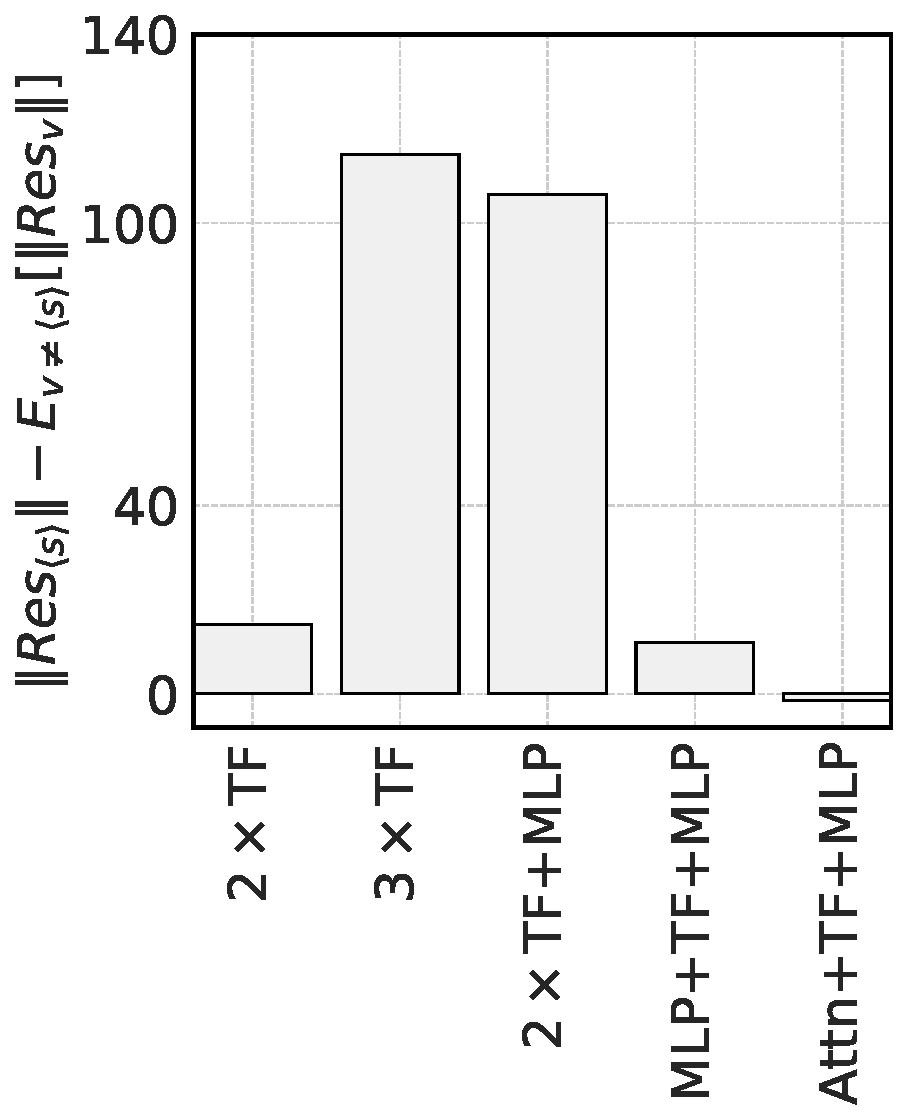
\includegraphics[width=0.3\linewidth]{Figures/BBM_appendix/massive_norm_minimal.pdf}
    \caption{\small Minimal structures to elicit residual state peaks. We use $A+B+C$ to indicate the model with structure $A$, $B$, $C$ in layers 0, 1, and 2, respectively.}
    \label{appfigure:massive_minimal}
\end{figure}



\subsection{Additional plots for the three-layer transformer trained on BB task}
\label{appsec:three-layer-tf}
We provide more results to the three layer transformer model trained on the BB task. They provide supporting evidence for the claim in Section~\ref{sec:res-peak}, stating that “Massive residual states amplify attention sinks and value-state drains in later layers.”
Figures \ref{appfigure:massive-attn}, \ref{appfigure:massive-value-norm}, and \ref{appfigure:massive-norm} show the extreme token phenomena in a three-layer transformer. The residual state peaks show different phenomena from those in LLMs, with the last layer output increasing the residual norms of non-\bos~tokens. Figure \ref{figure:extreme-token}
 demonstrates that the residual state norms of \bos~drop match the magnitudes of other tokens at the last layer. 
\begin{figure}[h]
  \centering
  \begin{minipage}{0.3\textwidth}
      \centering
      \subcaption{\small Layer 0}
      \vspace{-.2em}
      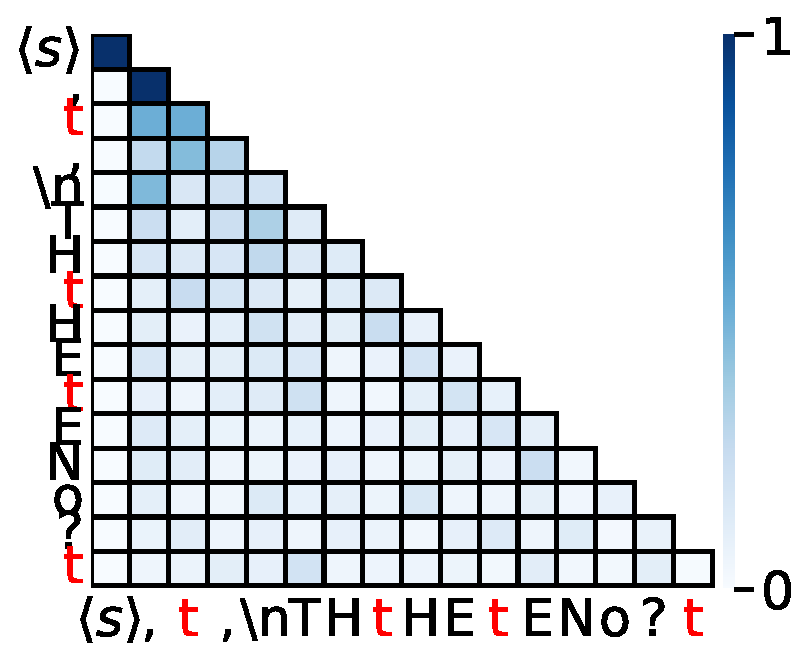
\includegraphics[width=\linewidth]{Figures/BBM_appendix/massive_attn_step10k_fig0.pdf}
  \end{minipage}
  % \hspace{-1em}
  \begin{minipage}{0.3\textwidth}
      \centering
      \subcaption{\small Layer 1}
      \vspace{-.2em}
      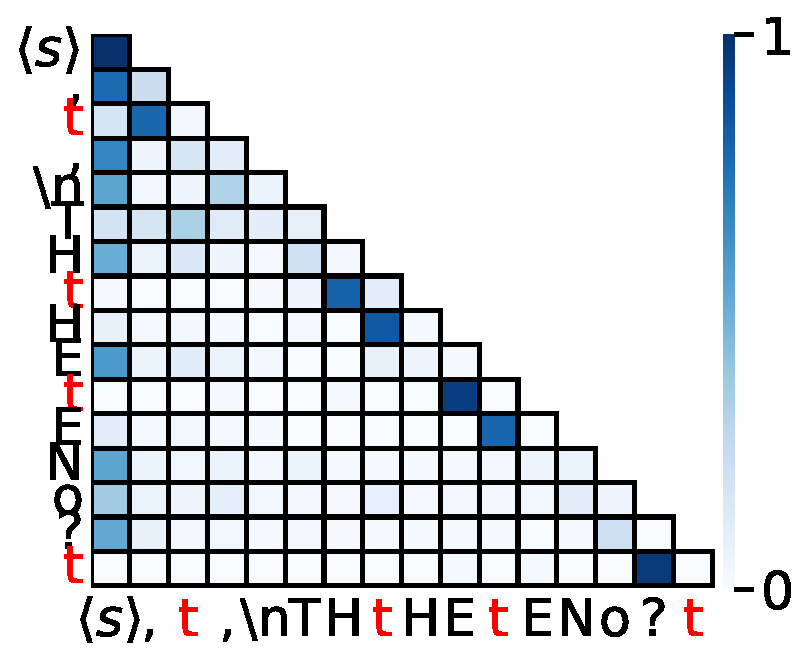
\includegraphics[width=\linewidth]{Figures/BBM_appendix/massive_attn_step10k_fig1.pdf}
  \end{minipage}
  % \hspace{-1em}
  \begin{minipage}{0.3\textwidth}
      \centering
      \subcaption{\small Layer 2}
      \vspace{-.2em}
      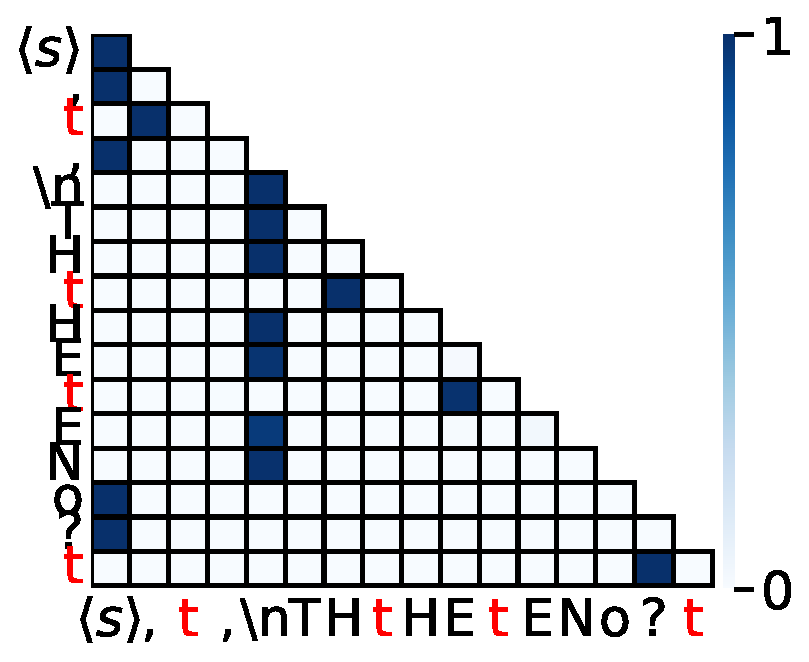
\includegraphics[width=\linewidth]{Figures/BBM_appendix/massive_attn_step10k_fig2.pdf}
  \end{minipage}
  % \vspace{-1em}
  \caption{\small Attention weight patterns of three-layer transformer trained on the BB task}
  \label{appfigure:massive-attn}
  \vspace{-1em}
\end{figure}

\begin{figure}[h]
  \centering
  \begin{minipage}{0.3\textwidth}
      \centering
      \subcaption{\small Layer 0}
      \vspace{-.2em}
      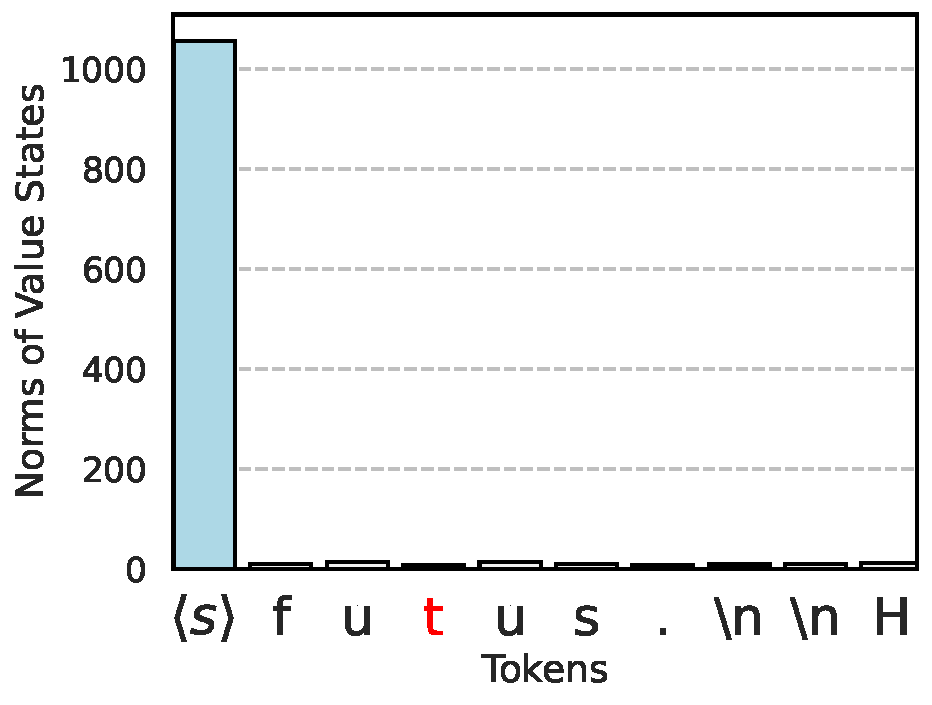
\includegraphics[width=\linewidth]{Figures/BBM_appendix/value_states_layer_0.pdf}
  \end{minipage}
  % \hspace{-1em}
  \begin{minipage}{0.3\textwidth}
      \centering
      \subcaption{\small Layer 1}
      \vspace{-.2em}
      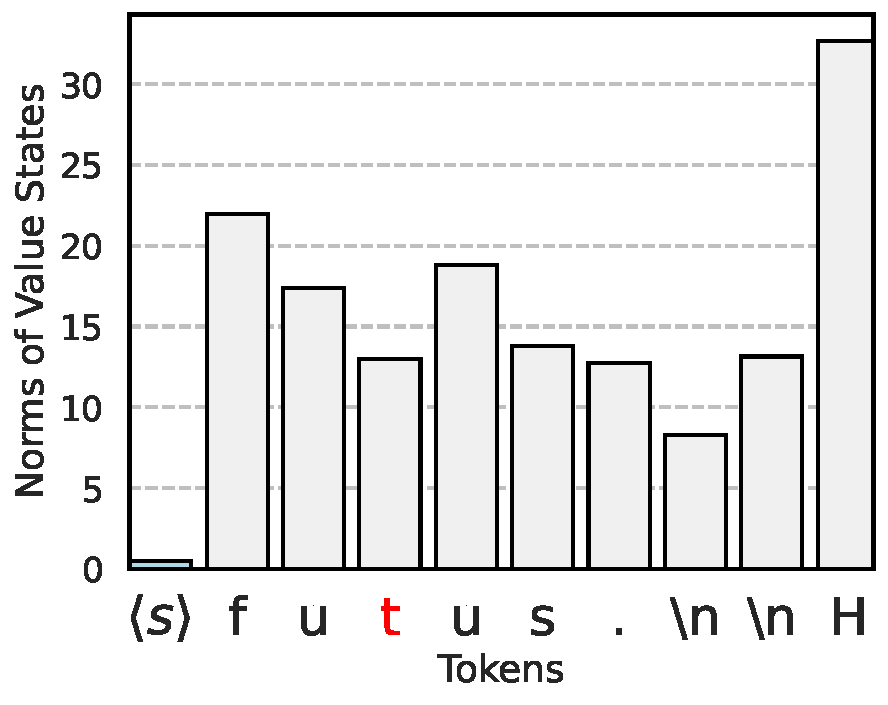
\includegraphics[width=\linewidth]{Figures/BBM_appendix/value_states_layer_1.pdf}
  \end{minipage}
  % \hspace{-1em}
  \begin{minipage}{0.3\textwidth}
      \centering
      \subcaption{\small Layer 2}
      \vspace{-.2em}
      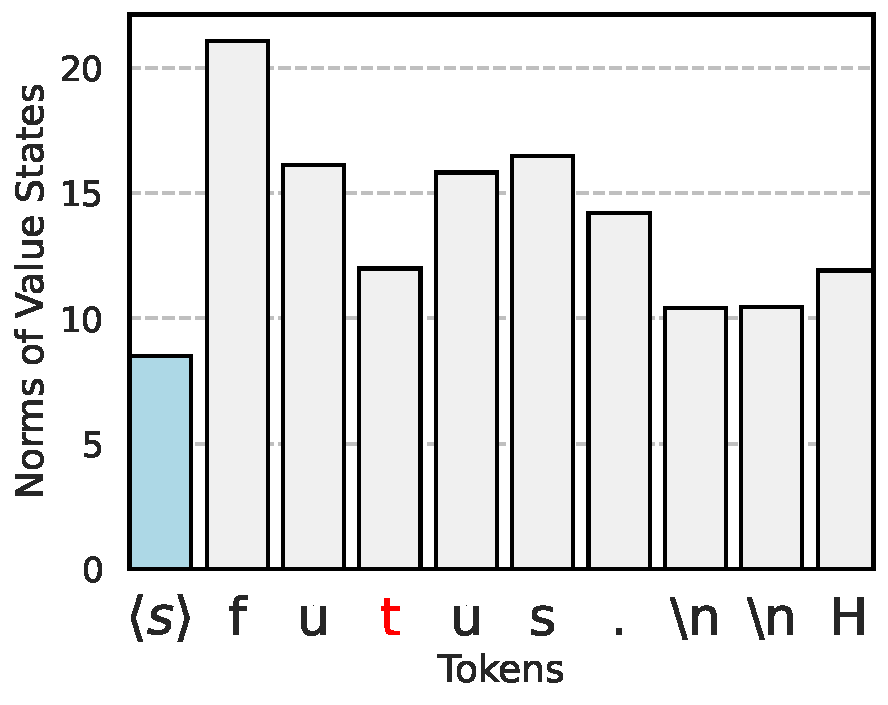
\includegraphics[width=\linewidth]{Figures/BBM_appendix/value_states_layer_2.pdf}
  \end{minipage}
  % \vspace{-1em}
  \caption{\small Value state norms of three-layer transformer trained on the BB task}
  \label{appfigure:massive-value-norm}
  \vspace{-1em}
\end{figure}


\begin{figure}[h]
  \centering
  \begin{minipage}{0.3\textwidth}
      \centering
      \subcaption{\small Layer 0}
      \vspace{-.2em}
      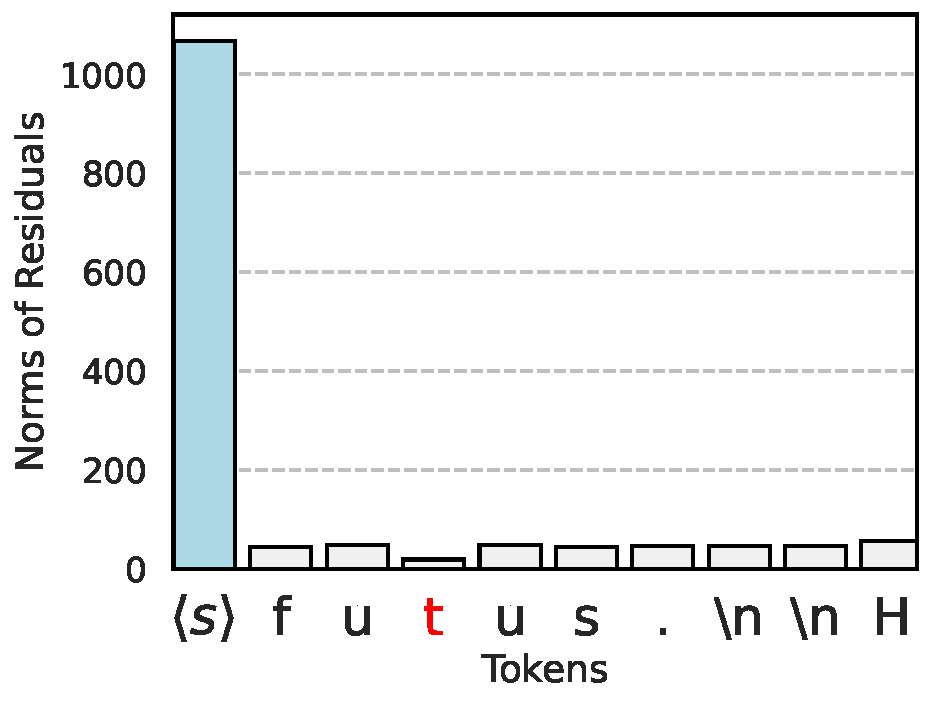
\includegraphics[width=\linewidth]{Figures/BBM_appendix/norms_layer_0.pdf}
  \end{minipage}
  % \hspace{-1em}
  \begin{minipage}{0.3\textwidth}
      \centering
      \subcaption{\small Layer 1}
      \vspace{-.2em}
      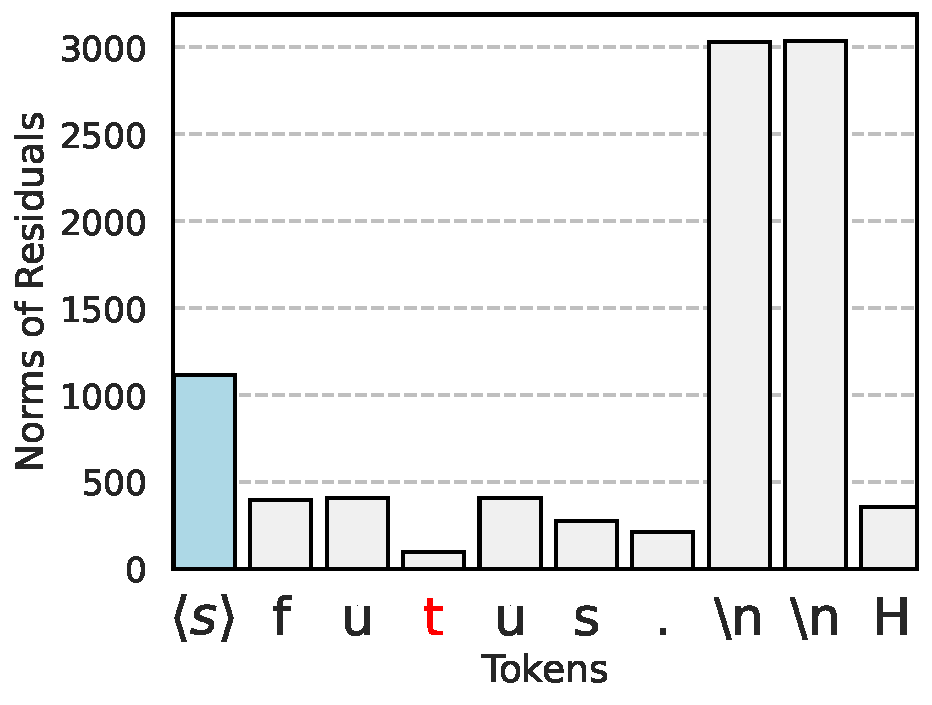
\includegraphics[width=\linewidth]{Figures/BBM_appendix/norms_layer_1.pdf}
  \end{minipage}
  % \hspace{-1em}
  \begin{minipage}{0.3\textwidth}
      \centering
      \subcaption{\small Layer 2}
      \vspace{-.2em}
      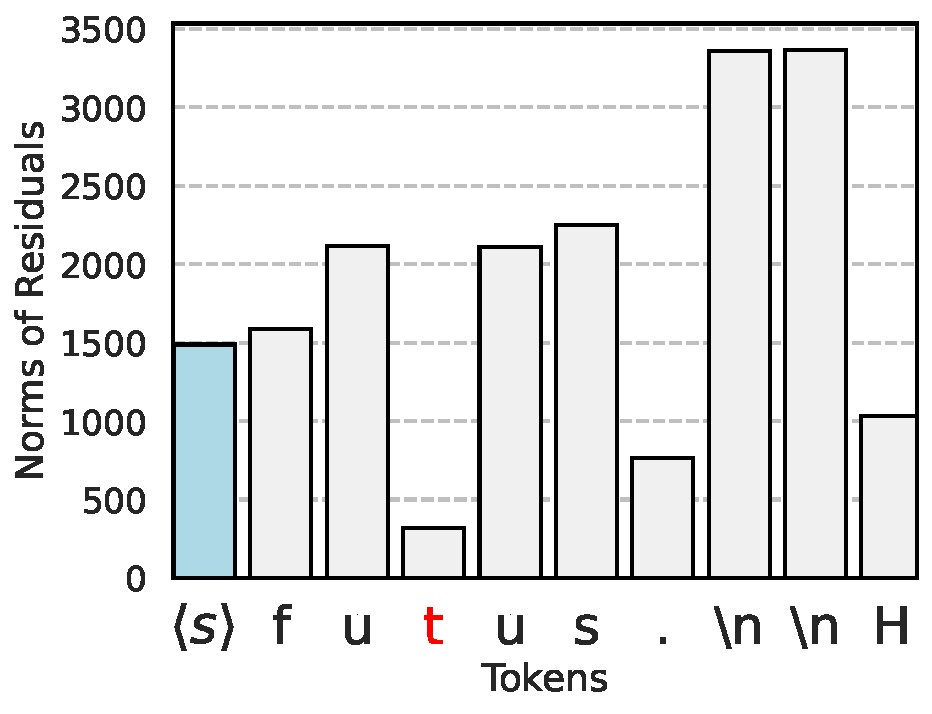
\includegraphics[width=\linewidth]{Figures/BBM_appendix/norms_layer_2.pdf}
  \end{minipage}
  % \vspace{-1em}
  \caption{\small Residual state norms of three-layer transformer trained on the BB task}
  \label{appfigure:massive-norm}
  \vspace{-1em}
\end{figure}


\subsection{Potential mechanism for linear growth of the residual state peak in multi-layer models}
\label{appsec:theory-for-res}
We give more details for the claim in Section~\ref{sec:res-peak}, stating that ``The ReLU attention and changing Adam to SGD eliminates the residual state peaks'' We first state Claim~\ref{sec:res-peak}.
\begin{claim}[Potential mechanism for the formation of residual-state peaks]\label{claim:res-peak}
In the training dynamic of a multi-layer transformer, if the mutual reinforcement mechanism (cf.\ Claim~\ref{claim:mutual-reinforcement}) occurs in upper layers:
\begin{enumerate}
    \item The gradients of $\res_\bos$ have the same direction (aligning with the null space of value matrices in upper layers and the $\key_\bos$) along the training dynamics.
    \item The layer-norm operations cause the fast decay of the magnitude of the gradients.
    \item Adam induces diminishing gradients to be constant updates, leading to the linear growth for the norm of the residual state of the extreme token.
\end{enumerate}
\end{claim}
To support the claim, we use the simplified model in Section~\ref{sec:bb_task}, including the residual state norm.
Denote the layer-norm operation as $\lnm$.
Heuristically, we can split the residual state $\res_{\bos}$ to a summation of two directions.
\[
\res_{\bos} = m \cdot \bm{\eta} + \bm{\eps},
\]
where $\bm{\eta},\bm{\eps} \in \R^\vocabsize$ with $\|\bm{\eta}\|_2=\|\bm{\eps}\|_2 = 1$, and $\bm{\eta}^\top \bm{\eps} = \rho>0$. The $\bm{\eta}$ corresponds to the direction of $\key_\bos$ in the original transformer, and $\bm{\eps}$ corresponds to other directions.
Assume that the attention logit from the token $\tok$ to the \bos~token in layer 1 is given by 
\begin{equation}\label{eqn:logits_in_residual_massive} \text{logit}_{\tok,\bos}= \sink_\tok = \Tilde{\sink}_\tok \bm{\eta}^\top \lnm(\res_{\bos})=\Tilde{\sink}_\tok \cdot \frac{m+\rho}{\sqrt{m^2+2m\rho+1}}.\end{equation}
We assume that the scalars $m$ and $\Tilde{\sink}$ are trainable, quantifying the norm of the residual states and magnitude of attention sinks. In the loss function $\loss_\tok$ as defined in Eq.~\eqref{eqn:loss_single}, we replace $\sink_\tok$ by the expression as in Eq.~(\ref{eqn:logits_in_residual_massive}), so that the loss function becomes a function of $(\Tilde{\sink}_\tok, \vecvalue, m)$, denoted as
\[
\wt{\loss}_\tok(\Tilde{\sink}_\tok, \vecvalue, m) = \loss_\tok(\sink_\tok, \vecvalue),
\]
We then consider the total loss as the average of the losses on each non-trigger token, weighted by its proportion in the stable distribution $\{\pi_v\}_{v \in \vocab}$, given by
\begin{equation}\label{appeqn:res_total_loss}
\wt{\loss}(\Tilde{\vecsink}, \vecvalue, m) = \sum_{\tok \in \vocab \setminus \cT} \stable_\tok \cdot \wt{\loss}_\tok(\Tilde{\sink}_\tok, \vecvalue, m).
\end{equation}
\begin{proposition}\label{appthm:massive}
% Consider the gradient flow of the loss function $\wt{\loss}(\Tilde{\vecsink}, \vecvalue, m)$. 
Assume $\xi_\tok\geq 0$ for any $\tok$, $\set{W_k\ivalue_k}_{k\in\vocab}$ are not all equal, and $\rho>0$. Fix $\vecvalue=\bm{0}$, and consider the gradient flow of $\wt{\loss}(\Tilde{\vecsink}, \vecvalue, m)$ over $\Tilde{\vecsink}$ and $m$. With any initial value $\Tilde{\sink}_\tok(0)>0$ for any $\tok$ and $m(0)>0$, we have that
\[
\dot{m}(t)=O\Big(\frac{\log t}{\sqrt{t} m^{3}}\Big).
\]
\end{proposition}
\begin{proof}[Proof of Proposition~\ref{appthm:massive}]
The chain rule gives that
\[
\dot{\Tilde{\sink}}_\tok(t) = \dot{\sink}_\tok \cdot \frac{m+\rho}{\sqrt{m^2+2m\rho+1}},
\]
and
\[
\dot{m}(t) = \sum_{\tok=1}^\vocabsize \Big\{\dot{\sink}_\tok \Tilde{\sink}_\tok \cdot \frac{\mathrm{d} \lnm(\res_\bos)}{\mathrm{d} t} \Big\}.
\]
With the initial values, $\dot{m}(t)\geq 0$ and $\dot{\Tilde{\sink}}_\tok(t) \geq 0$.
We have $m(t)\geq 0$ for any $t$. Hence, $$\dot{\Tilde{\sink}}_\tok \in [\rho \dot{\sink}_\tok,  \dot{\sink}_\tok].$$ 
Therefore, $\Tilde{\vecsink} = 2^\inv \log t \bm{1} + \Tilde{\bm{r}}(t)$ with $\Tilde{\bm{r}}(t)$ uniformly bounded over time. Furthermore, we have that
\begin{align*}
\dot{m}(t) & = \sum_{\tok=1}^\vocabsize \Big\{\dot{\sink}_\tok \Tilde{\sink}_\tok \cdot \frac{\mathrm{d} \lnm(\res_\bos)}{\mathrm{d} t} \Big\}\\
& = O\Big(\frac{\log t}{\sqrt{t}}\Big) \cdot \frac{1-\rho^2}{(m^2+2m\rho+1)^{3/2}}\\
& = O\Big(\frac{\log t}{\sqrt{t}m^3}\Big).
\end{align*}
This proves Proposition~\ref{appthm:massive}.
\end{proof}
We use simulation to demonstrate the effect of Adam. We train the scalar $m$ using Adam with gradient $\mathrm{d}m = \log t / [\sqrt{t}m^3]$. We set $\beta_1=0.9$, $\beta_2=0.999$, weight decay$=10^{-8}$, and the learning rate $\text{lr}=0.3$. Figure~\ref{appfigure:m_dynamics} presents the training dynamics of $m$. We observe the linear growth after a warming-up phase. In contrast, when trained by SGD with learning rate $\text{lr}=0.3$, $m$ remains small. The results match transformer models on BB-task as in Figure~\ref{fig:sgd}.

\begin{figure}[h]
    \centering
    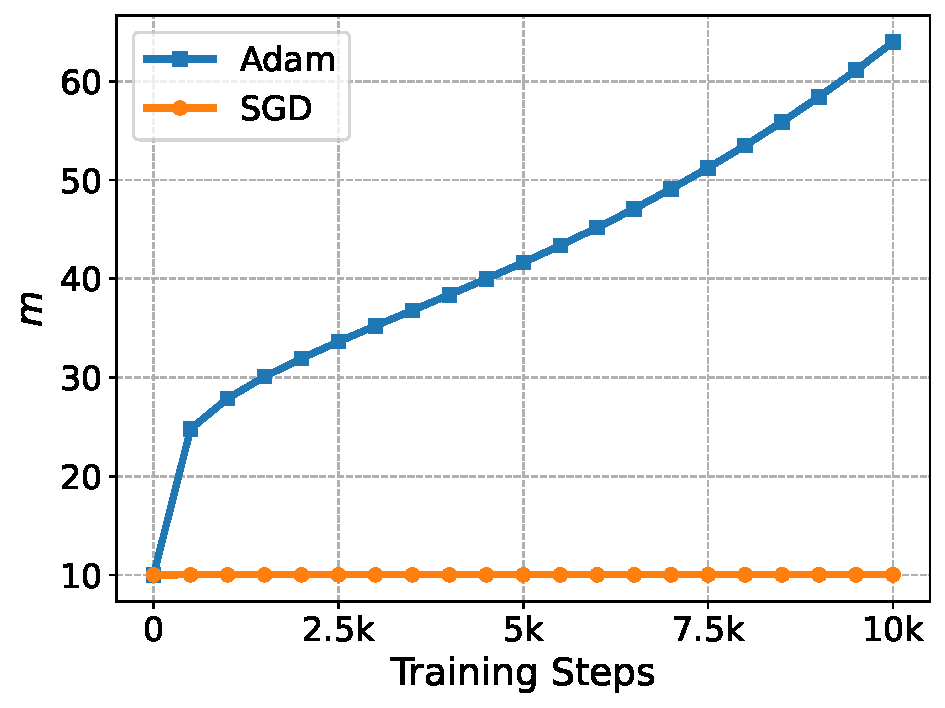
\includegraphics[width=0.5\linewidth]{Figures/BBM_appendix/m_dynamics.pdf}
    \caption{With the gradient formula in Proposition~\ref{appthm:massive}, Adam causes linear growth of $m$. 
    % \tianyu{put SGD plot here}
    }
    \label{appfigure:m_dynamics}
\end{figure}
\clearpage
\begin{table}[h]
    % \captionsetup{font=small}
    \small
    \centering
    % \vspace{-1em}
    \caption{\label{table:ablations} Perplexity of SSM variants compared to
      Transformers on OpenWebText. All models have 12 layers, with size around 125M, and are trained
      with the same hyperpameters, for 50B tokens.}
    %   \vspace{1em}
    {
        \begin{tabular}{@{}|ccccc|c|@{}}
            \hline
        %   \specialrule{.15em}{.05em}{.05em}
        \hthree & \hthree Hybrid (2 Attn) & S4D & GSS & GSS Hybrid (2 Attn) & Transformer  \\ % & Training time \\
        %   \specialrule{.15em}{.05em}{.05em}
        \hline
        21.0 & \textbf{19.6} & 24.9 & 24.0 & 19.8 & 20.6 \\ \hline
        \end{tabular}
    }
    % \vspace{-1.5em}
\end{table}
\clearpage
\section{More Attention Heads in Dormant and Active Phase}\label{sec:more_heads}
We demonstrate a head with clear \textit{active-dormant mechanism} in Figure~\ref{fig:dormant_heads_domain_dependent}. 
In this section, we present two more active-dormant heads in Llama 2-7B-Base, in \Cref{fig:llama_l16h20,fig:llama_l16h28}, which are more difficult to interpret than Layer 16 Head 25, but become dormant on some inputs and remain active on others. 
% \sm{Explain in more details. Now the figure is far away from the text. }

\begin{figure}[h]
    \centering
    \begin{subfigure}{0.575\textwidth}
        \centering 
        \caption{Attention patterns}
        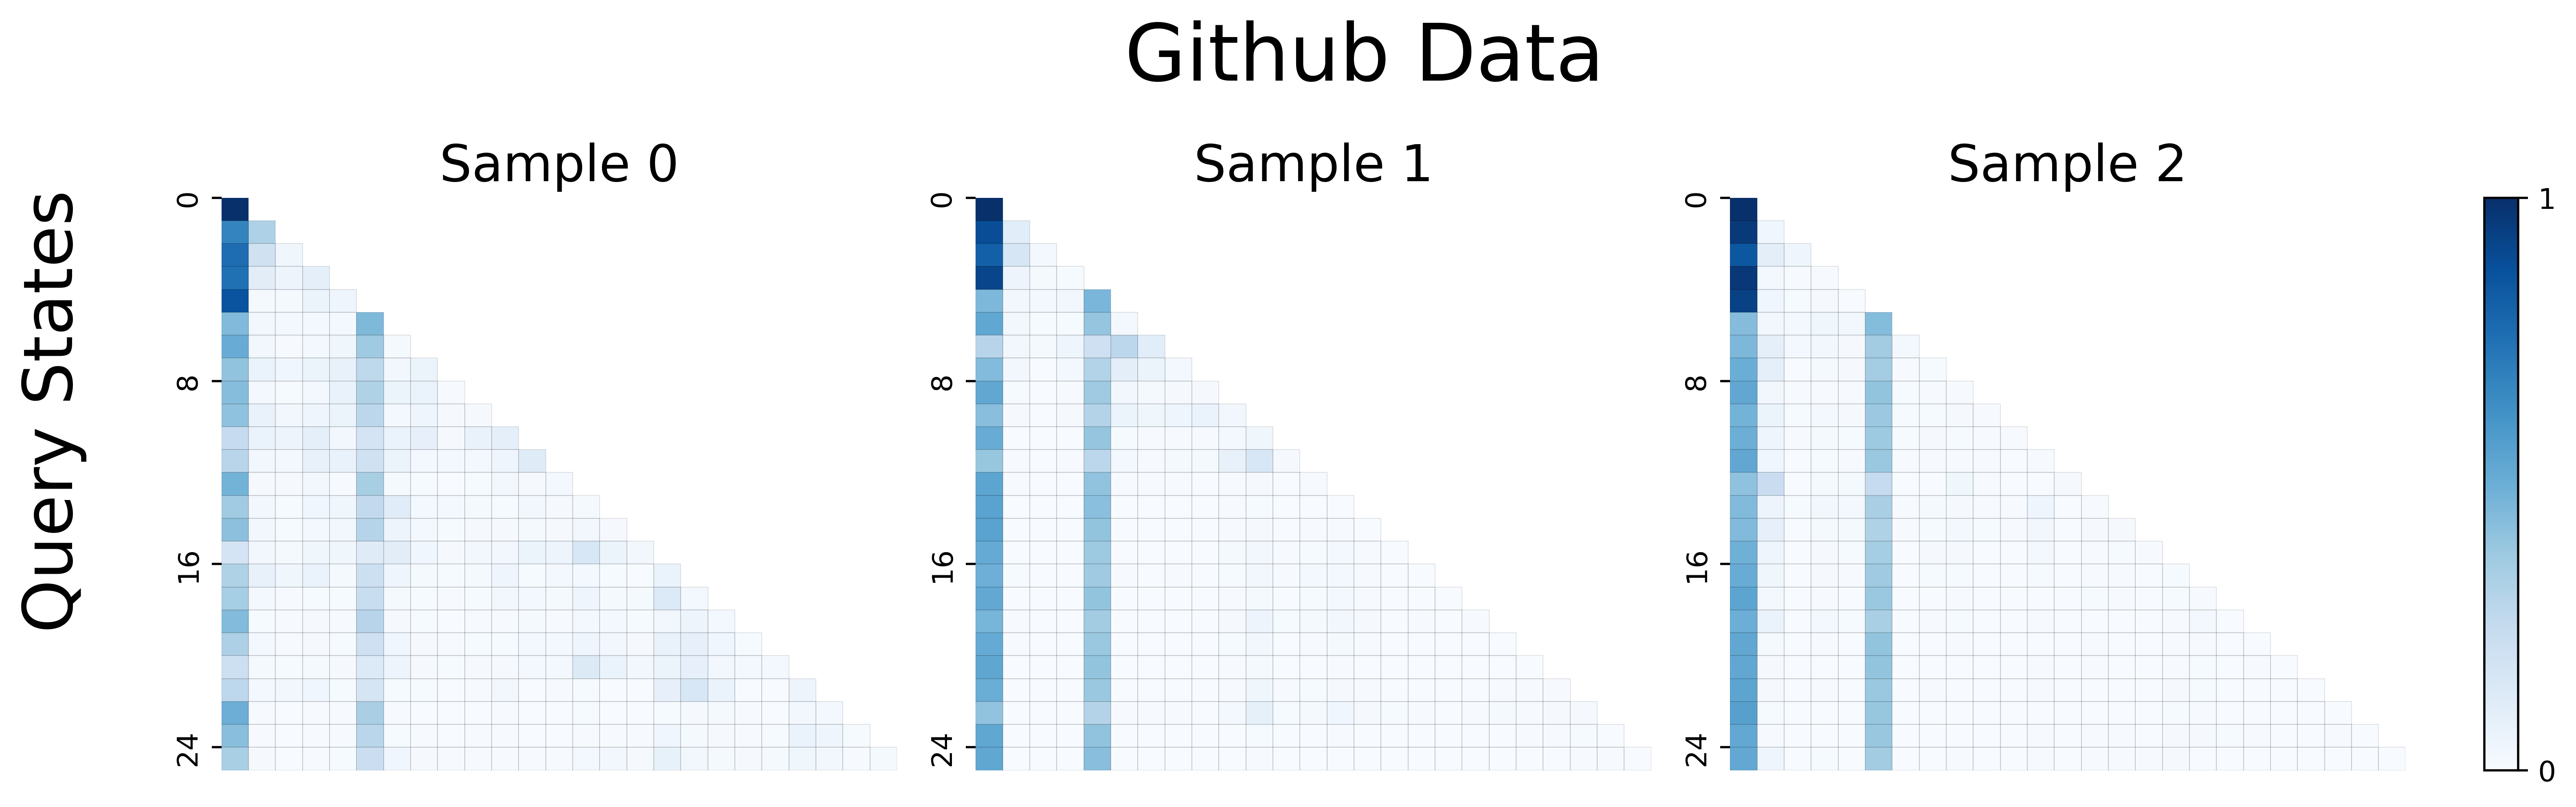
\includegraphics[width=\linewidth]{Figures/L16H20/attn_github_head20.png}
        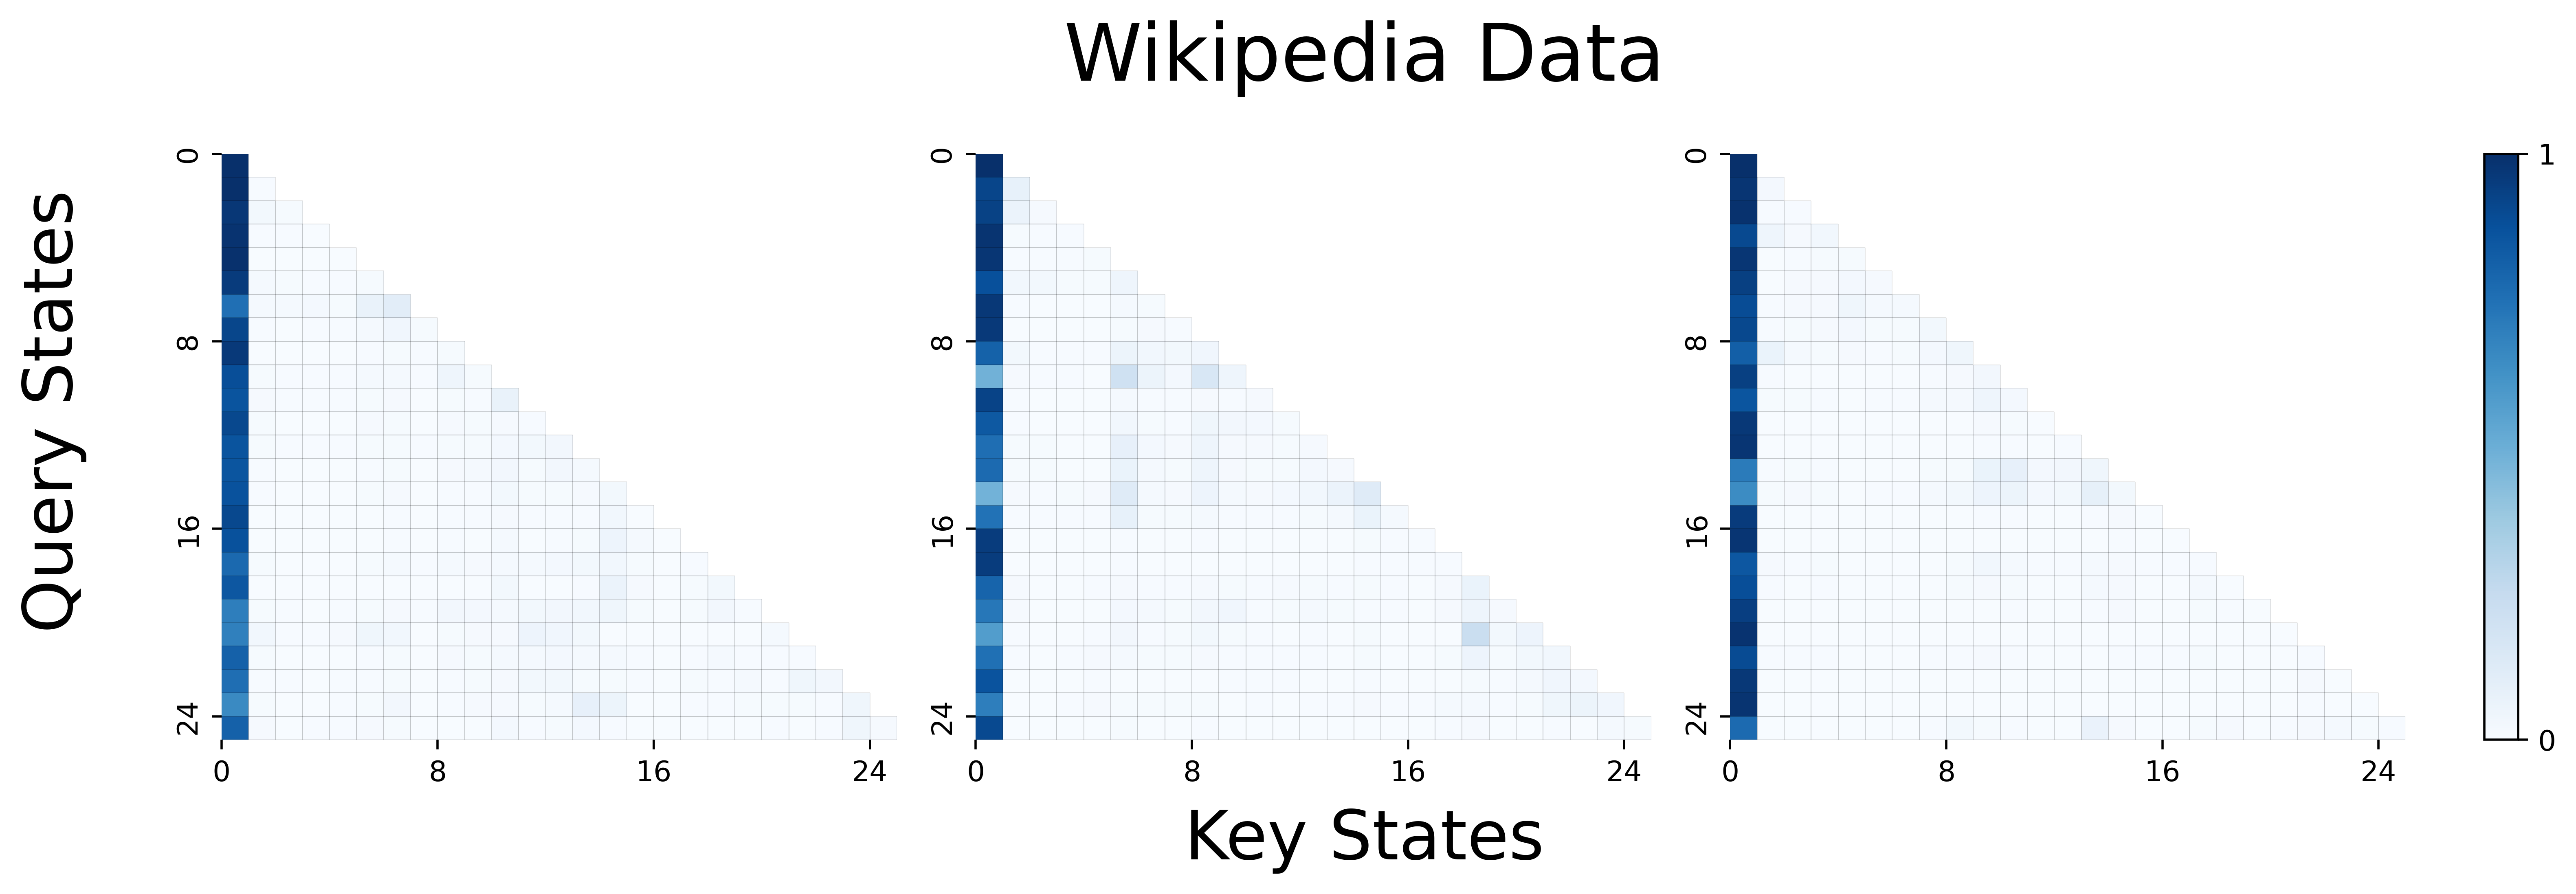
\includegraphics[width=\linewidth]{Figures/L16H20/attn_wikipedia_head20.png}
    \end{subfigure}
    \hfill
    \begin{subfigure}{0.4\textwidth}
        \centering
        \caption{Interventions}
        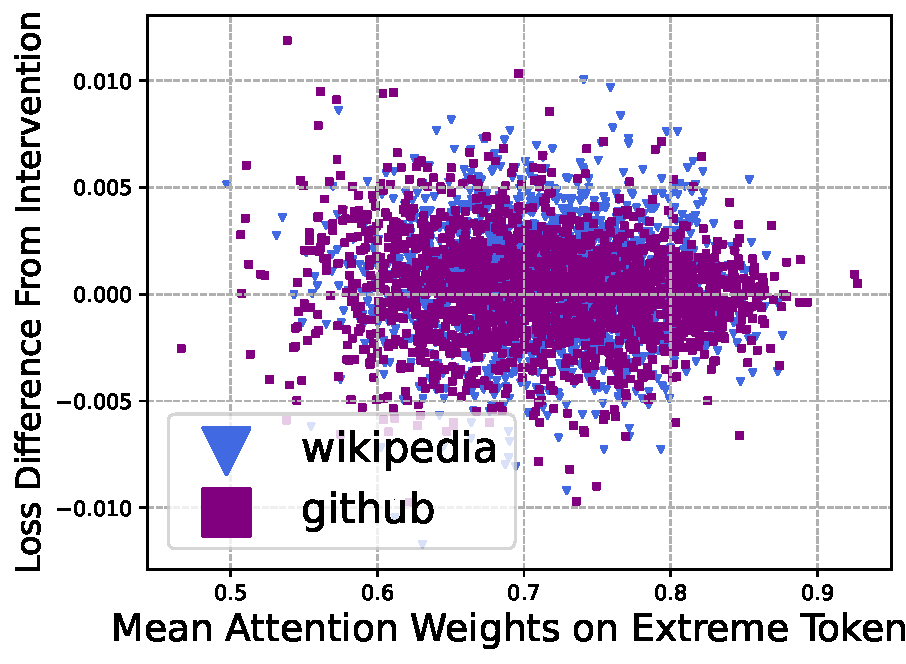
\includegraphics[width=\linewidth]{Figures/L16H20/L16H20.pdf}
    \end{subfigure}
    \caption{\small \textbf{Layer 16 Head 20 of Llama 2-7B-Base.} We do not observe difference between the Wikipedia data and the Github data.}
    \label{fig:llama_l16h20}
\end{figure}

\begin{figure}[h]
    \centering
    \begin{subfigure}{0.575\textwidth}
        \centering
        \caption{Attention patterns}
        \includegraphics[width=\linewidth]{Figures/L16H28/attn_github_head28.png}
        \includegraphics[width=\linewidth]{Figures/L16H28/attn_wikipedia_head28.png}
    \end{subfigure}
    \begin{subfigure}{0.4\textwidth}
        \centering
        \caption{Interventions}
        \includegraphics[width=\linewidth]{Figures/L16H28/L16H28.pdf}
    \end{subfigure}
    \caption{\small \textbf{Layer 16 Head 28 of Llama 2-7B-Base.} The head is more dormant on the GitHub data, and more active on the Wikipedia data.}
    \label{fig:llama_l16h28}
\end{figure}



\clearpage
\section{Fine-Grained Static Mechanisms for Extreme-Token Phenomena} \label{sec:circuit}

In this section, we identify more fine-grained static mechanisms for extreme-token phenomena in Llama 3.1-8B-Base. To do this, we identify circuits for the origin of attention sinks and small value states. Then, using ablation studies, we study the origin of massive norms. Again, we use the generic test phrase ``\bos{} Summer is warm. Winter is cold.''

\begin{figure}[h]
    \centering
    \includegraphics[width=0.8\textwidth]{Figures/llama_31_circuit/demo_attn_heads.pdf}
    \caption{\small \textbf{A visualization of attention heads at Layer 0 of Llama 3.1-8B-Base.} Notice that many heads have the attention sink property, even at Layer 0 without any cross-token interaction. As usual, the test phrase is ``Summer is warm. Winter is cold.'' The most clear attention sink is Head 31.}
    \label{fig:llama_31_attn_layer0}
\end{figure}

\begin{figure}[h]
    \centering
    \begin{subfigure}[t]{0.4\textwidth}
    \caption{Correlations between key and query states.}
        \centering
        \includegraphics[width=0.6\textwidth]{Figures/llama_31_circuit/demo_qkt.pdf}
    \end{subfigure}
    \quad
    \begin{subfigure}[t]{0.4\textwidth}
        \centering
        \caption{Correlations between key states.}
        \includegraphics[width=0.6\textwidth]{Figures/llama_31_circuit/demo_kkt.pdf}
    \end{subfigure}
    \caption{\small \textbf{Correlations between query states and key states at Layer 0 Head 31 of Llama 3.1-8B-Base.} We observe that the key state of \bos{} have low correlation with other key states, but high correlation with other query states. Meanwhile, all semantically meaningful (i.e., not delimiter) tokens have highly correlated key states.}
    \label{fig:llama_31_qk_kk}
\end{figure}

\paragraph{Attention sinks and global contextual semantics.} There are many attention heads that exhibit attention sinks at layer \(0\), and the \bos{} token is always the sink token (see \Cref{fig:llama_31_attn_layer0}). From now on until the end of this section, we restrict our attention to Head 31 of Layer 0, which is an attention sink. These attention sinks are caused by two linear-algebraic factors, demonstrated in \Cref{fig:llama_31_qk_kk}.
\begin{enumerate}
    \item The key state of the \bos{} token has small dot product with all other key states. 
    \item The query states of all tokens are nearly orthogonal to the key states of all tokens except the \bos{} token.
\end{enumerate}
 These two facts combine to ensure that the key state of the \bos{} token is picked out by each query state, causing the attention sink. Since these query and key states are produced without any cross-token interaction, the alignment of different states is caused purely by the token's global importance or meaning imparted via pretraining. The \bos{} token has no semantic meaning in the context of prose tokens, so its key state is not aligned with key states of meaningful prose tokens. Also, delimiter tokens, often considered secondary attention sinks (cf.~\Cref{sub:fixed_bos}), have the most aligned key states to the key state of the \bos{} token, and are also the tokens with the least semantic meaning in the prose context. Thus, we identify that, at least in this restricted example, query state and key state alignment depends heavily on the contextual semantics of the token.

 \begin{figure}[h]
     \centering
     
     \begin{subfigure}[t]{0.3\textwidth}
        \centering
        \caption{Value-state drains at Layer 0 Head 31 of Llama 3.1-8B-Base.}\label{fig:llama_31_value_states}\includegraphics[width=0.9\textwidth]{Figures/llama_31_circuit/demo_val_norms_head_31.pdf}
    \end{subfigure}
    \begin{subfigure}[t]{0.6\textwidth}
    \centering
        \caption{\centering Ablation study on the cause of the residual state peak in Llama 3.1-8B-Base.}\label{fig:llama_31_norms_ablation}\includegraphics[width=0.5\textwidth]{Figures/llama_31_circuit/res_intervention.pdf}
    \end{subfigure}
    
     \caption{\small \textit{Left (a)}: Value-state drains at Layer 0 Head 31 of Llama 3.1-8B-Base. We observe that the value state associated with \bos{} is already much smaller than every other semantically meaningful token, and still smaller than the delimiter tokens in the same sentence. \textit{Right (b)}: Ablation study on the cause of the residual state peak in Llama 3.1-8B-Base. We perform a series of ablations to understand which components of the network promote the residual state peaks. We find that ablating either the zeroth or first layer's MLP is sufficient to remove the residual state peak phenomenon, while no other layer-level ablation can do it.}
     \label{fig:llama_31_value_states and norms}
 \end{figure}

\paragraph{Value-state drains.} The value states of the \bos{} token at Layer \(0\) Head 31 are already near zero, as demonstrated in \Cref{fig:llama_31_value_states}. While the delimiter tokens, which are less semantically meaningful in the prose context, have smaller value states than the rest, they are not as small as the value state of the \bos{} token which is guaranteed to not have any semantics.

% \begin{figure}[h]
%     \centering
%     \includegraphics[width=0.4\textwidth]{Figures/llama_31_circuit/llama_31_massive_norms.png}
%     \caption{\small\textbf{Ablation study on the cause of the residual state peak in Llama 3.1-8B-Base.} We perform a series of ablations to understand which components of the network promote the residual state peaks. We find that ablating either the zeroth or first layer's MLP is sufficient to remove the residual state peak phenomenon, while no other layer-level ablation can do it. \sm{Put together with} \tianyu{add links back to Section D}}
%     \label{fig:enter-label}
% \end{figure}

\paragraph{Residual state peaks.} Residual state peaks are caused by the first two layers' MLPs. In particular, we perform several ablations, comparing between the residual state norms in a later layer (\(24\)) of an un-edited forward pass versus forward passes where we force the output of either multiple layers, a single layer, an attention block, or an MLP to be zero (and hence remove its contribution from the residual stream). As shown in Figure~\ref{fig:llama_31_norms_ablation}, ablating \textit{either} Layer 0's or Layer 1's MLP is sufficient to remove the residual state peak. In particular, the second-largest token at Layer 24 in \textit{each} ablation (including the original setup) has norm between \(29\) and \(38\), so the interventions ensure that all tokens have similar size.

% \begin{figure}
%     \centering
%     \begin{subfigure}[t]{0.24\textwidth}
%         \centering 
%         \caption{\small Attention sinks (L0).}
%         \includegraphics[width=\textwidth]{Figures/llama_31_circuit/llama_31_attn_l0.png}
%         \label{fig:llama_31_attn_sink_l0}
%     \end{subfigure}
%     \begin{subfigure}[t]{0.32\textwidth}
%         \centering 
%         \caption{\small Value norms (L0H31).}
%         \includegraphics[width=\textwidth]{Figures/llama_31_circuit/llama_31_value_l0.png}
%         \label{fig:llama_31_v_l0}
%     \end{subfigure}
%     \begin{subfigure}[t]{0.49\textwidth}
%         \centering 
%         \caption{\small Correlations between query/key states (L0H31).}
%         \includegraphics[width=0.49\textwidth]{Figures/llama_31_circuit/llama_31_qk_l0.png}
%         \includegraphics[width=0.49\textwidth]{Figures/llama_31_circuit/llama_31_kk_l0.png}
%         \label{fig:llama_31_qk_kk_l0}
%     \end{subfigure}
%     \begin{subfigure}[t]{0.24\textwidth}
%         \centering 
%         \caption{\small Res.~stream ablations.}
%         \includegraphics[width=\textwidth]{Figures/llama_31_circuit/llama_31_massive_norm.png}
%         \label{fig:llama_31_resid_l0}
%     \end{subfigure}
    
%     %\includegraphics[width=0.5\linewidth]{}
%     \caption{\small \textbf{A circuit for extreme-token phenomena in Llama 3.1-8B-Base.} \textit{Top:} Attention sinks present in Layer 0. \textit{Left:} Value states of tokens which are semantically irrelevant for prose are small, and the \bos{} token (which is always semantically irrelevant) is the smallest. Since these value states are in the zeroth layer, they have not been computed via any cross-token interaction, so this is a result about how tokens align with the value weight matrix as per their usefulness. \textit{Middle:} In the first layer, attention sinks form because key states of semantically irrelevant tokens are correlated with all query states, while other key states are nearly orthogonal to all query states. Meanwhile, all semantically relevant key states are nearly orthogonal to semantically irrelevant key states, and are very aligned with each other. Again, the query and key states were computed in the zeroth layer and so without any previous cross-token interaction, so this shows how the zeroth-layer query and key weight matrices align to tokens depending on their semantic meaning as inferred by pretrraining. \textit{Right:} Residual state peaks are present due to the MLPs in the first two layers: ablating either of them by manually removing their contribution to the residual stream is sufficient to remove the residual-state peaks, but ablating any other components will preserve the residual state peak phenomenon. % Evidence of a circuit for massive norm, attention sink, value states in Llama 3.1
%     %\DP{TODO: left figure is show a few attention heatmaps, like 4 or 8; middle figure is show Q dot K, K dot K, and value norms; right figure is residual norm}
%     }
%     \label{fig:llama_31_circuits}
% \end{figure}

\clearpage
\section{Extreme-Token Phenomena Over Many Samples}\label{sec:many_samples}
In this section we show that the extreme-token phenomena, and our predictions from the BB model, exhibit in prompts other than ``Summer is warm. Winter is cold.'' To this end, we use 128 samples from the Wikipedia dataset, each truncated to 8 tokens. \Cref{fig:extreme_tokens_llama_31_many_samples} provides aggregate statistics of extreme-token phenomena in Llama 3.1-8B, which are similar to the fine-grained statistics over a single prompt from \Cref{figure:extreme-token}. \Cref{fig:extreme_tokens_olmo_many_samples} provides aggregate statistics of the development of extreme-token phenomena over the training dynamics of OLMo, which are similar to the fine-grained statistics over a single prompt from \Cref{fig:olmo_predictions_phase0} and \Cref{fig:olmo_predictions_phase1}.


\begin{figure}[h]
    \centering
    \begin{subfigure}{0.31\textwidth}
        \centering 
        \caption{Attention weights (L24).}
        \includegraphics[width=\textwidth]{Figures/more_samples_statics/attn_weights_k_tokens.pdf}
    \end{subfigure}
    \hfill
    \begin{subfigure}{0.31\textwidth}
    \centering 
    \caption{Value state norms.}
    \includegraphics[width=\textwidth]{Figures/more_samples_statics/val_drain_batch.pdf}
    \end{subfigure}
        \hfill
    \begin{subfigure}{0.32\textwidth}
        \caption{Residual norms.}
        \includegraphics[width=\textwidth]{Figures/more_samples_statics/res_peak_batch.pdf}
    \end{subfigure}
    
    \caption{\textbf{Extreme token phenomena over many samples in Llama 3.1-8B-Base.} \textit{Left (a):} Let \(A\) be the attention weight tensor, of shape \((\text{batch size=128, \# heads=32, \# tokens=8, \# tokens=8})\) at Layer 24 of Llama 3.1-8B-Base. We calculate the tensor \(\bar{A}\), of shape \((\text{batch size=128, \# heads=32, \# tokens=8})\), which measures the average attention mass on the key tokens, by the following calculation: \(\bar{A}_{bhj} \doteq \frac{1}{n-j}\sum_{i = j}^{n}A_{bhij}\). We expect, for an attention sink head \(h\) on sample \(b\), that \(\bar{A}_{bh0}\) is large, and \(\bar{A}_{bhj}\) is small for all \(j \geq 1\). We indeed see this by plotting the distribution of \(\bar{A}_{:, :, j}\) for each \(j\), which shows that almost all attention mass is concentrated on the \bos token with high probability, showing the same thing as the individual attention head analysis in \Cref{figure:extreme-token} (a). \textit{Middle (b), Right (c):} We do the same computations as \Cref{figure:extreme-token} (b) and (c), averaged over the \(128\) samples.}
    \label{fig:extreme_tokens_llama_31_many_samples}
\end{figure}

\begin{figure}
    \centering
    \begin{subfigure}{0.45\textwidth}
    \centering 
    \caption{Attention weights (L24).}
    \includegraphics[width=0.7\textwidth]{Figures/olmo_batch/attn_mass_on_top_two_tokens.pdf}
    \end{subfigure}
    % \hfill
    \begin{subfigure}{0.45\textwidth}
    \centering 
    \caption{Attention logits (L24).}
    \includegraphics[width=0.7\textwidth]{Figures/olmo_batch/attention_logits.pdf}
    \end{subfigure}
    
    \begin{subfigure}{0.45\textwidth}
    \centering 
    \caption{Value state norms (L24).}
    \includegraphics[width=0.7\textwidth]{Figures/olmo_batch/value_norms.pdf}
    \end{subfigure}
    % \hfill
    \begin{subfigure}{0.45\textwidth}
    \centering 
    \caption{Residual norms (L24).}
    \includegraphics[width=0.7\textwidth]{Figures/olmo_batch/layer_output_norms.pdf}
    \end{subfigure}

    \caption{\small \textbf{Dynamics of extreme-token phenomena in layer 24 over many samples in the training trajectory of OLMo-7B.} For this experiment, as in \Cref{sub:olmo_dynamics}, for each sample and attention head we designate two attention sink tokens as the two tokens with the largest average attention mass \(\bar{A}_{bhj}\) (see \Cref{fig:extreme_tokens_llama_31_many_samples} for definition). We then study the dynamics of sink tokens versus non-sink tokens. In these experiments we observe that token \(0\) is (almost) always a sink token, which we discuss further in \Cref{sub:fixed_bos}. \textit{Top left (a):} The average attention scores \(\bar{A}_{bhj}\) for \(j\) as a sink token versus non-sink tokens. We observe that attention sinks form in nearly all heads and samples: the attention mass on top tokens nearly always sums to \(1\), and moreover the sinks develop relatively early in training. \textit{Top right (b):} We observe that the normalized attention logits of non-sink tokens initially increase until the formation of an attention sink, and then approximately converge to a stable phase with similar logits on token \(0\). \textit{Bottom left (c):} We observe that the value states of all tokens except the first sink token (token \(0\)) rapidly converges to steady state, while the first sink token has a much lower value state norm than all other tokens. \textit{Bottom right (d)}: We observe that the norm of the residual state of token \(0\) increases linearly during pretraining, while all other tokens' residual states do not. Our results mirror and confirm the single-sample detailed analysis conducted in \Cref{sub:olmo_dynamics}.}
    \label{fig:extreme_tokens_olmo_many_samples}
\end{figure}

\clearpage
\section{Assorted Caveats}\label{sec:caveats}

\subsection{Multiple Attention Sinks vs. One Attention Sink}\label{sub:multiple_sinks_discussion}

As we have seen, attention heads in the BB task (\Cref{sec:bb_task}), Llama 2-7B-Base (\Cref{sub:active_dormant}), and OLMo (\Cref{sub:olmo_dynamics}) exhibit multiple attention sinks. That is, when heads in these models are dormant, they tend to have two attention sinks. For the LLMs in this group, at least on prose data, the \bos~token as well as the first delimiter token (e.g., representing \texttt{.} or \texttt{;}) are sink tokens. Meanwhile, Llama-3.1-8B-Base (\Cref{sec:llm}) only ever has one attention sink on prose data, and the \bos{} token is always the sink token. Here, we offer a possible explanation of this phenomenon. For the BB task, multiple sink tokens are necessary to solve the task. For LLMs, we believe this distinction may be explained by the relative proportion of coding data, in which delimiters have a greater semantic meaning than prose, within the training set. For instance, OLMo was trained on DOLMA \citep{soldaini2024dolma}, which has around 411B coding tokens. Meanwhile, Llama 2 used at most (2T \(\times\) 0.08 =) 0.16T coding tokens. Finally, Llama 3.1 used around (15.6T \(\times\) 0.17 =) 2.6T coding tokens \citep{dubey2024llama}. On top of the raw count being larger, coding tokens are a larger proportion of the whole pre-training dataset for Llama 3.1 compared to other model families. Thus, during training, the presence of delimiters would not be considered unhelpful towards next-token prediction, since such delimiters carry plenty of semantics in a wide variety of cases. Our earlier hypothesis in \Cref{sub:active_dormant} proposes that only tokens which lack semantics in almost all cases are made to be sink tokens. This could be a reason for the distinction.

\subsection{The Role of a Fixed \bos~ Token in the Active-Dormant Mechanism}\label{sub:fixed_bos}

\begin{figure}
    \centering
    \includegraphics[width=\textwidth]{Figures/bos_study/attn_heads_shuffled.png}
    \caption{\small \textbf{Attention sinks with shuffled input in Layer 24 of OLMo.} In order to understand the impact of positional encodings when there is no \bos{} token, we shuffle the input of the test string ``Summer is warm. Winter is cold.'' in OLMo. We observe that there is still an attention sink on token \(0\), despite it being a random token that does not usually start sentences or phrases (since it is uncapitalized). This shows that the positional embedding, say via RoPE, has a large impact on the formation of attention sinks --- when the semantics of each token have switched positions, the attention sink still forms on the zeroth token.}
    \label{fig:bos_shuffle}
\end{figure}

Some models, such as OLMo, are not trained with a \bos{} token. Despite this, the first token of the input still frequently develops into a sink token. We can study the effect of positional encoding of the tokens on the attention sink phenomenon by shuffling the tokens before inputting them into the transformer, and observing how and why attention sinks form. If we do this with the phrase ``Summer is warm. Winter is cold.'' with OLMo, we observe that at Layer 24, there are many attention sink heads where the first token and first delimiter token share attention mass, even if the sentence is jumbled up and makes no grammatical sense. This points towards the observation that without a \bos{} token, the attention sink formation uses both positional data and, to a greater degree, the semantic data of each token. We leave studying this effect in greater detail to future work.


% \DP{Add ablation experiments with RoPE. It should work since that is the only place which has positional information.}


% \subsection{The attention logits on non-bos tokens decrease through the training dynamics}





\end{document}
